\documentclass[twoside]{book}

% Packages required by doxygen
\usepackage{fixltx2e}
\usepackage{calc}
\usepackage{doxygen}
\usepackage[export]{adjustbox} % also loads graphicx
\usepackage{graphicx}
\usepackage[utf8]{inputenc}
\usepackage{makeidx}
\usepackage{multicol}
\usepackage{multirow}
\PassOptionsToPackage{warn}{textcomp}
\usepackage{textcomp}
\usepackage[nointegrals]{wasysym}
\usepackage[table]{xcolor}

% NLS support packages
platex
% Font selection
\usepackage[T1]{fontenc}
\usepackage[scaled=.90]{helvet}
\usepackage{courier}
\usepackage{amssymb}
\usepackage{sectsty}
\renewcommand{\familydefault}{\sfdefault}
\allsectionsfont{%
  \fontseries{bc}\selectfont%
  \color{darkgray}%
}
\renewcommand{\DoxyLabelFont}{%
  \fontseries{bc}\selectfont%
  \color{darkgray}%
}
\newcommand{\+}{\discretionary{\mbox{\scriptsize$\hookleftarrow$}}{}{}}

% Page & text layout
\usepackage{geometry}
\geometry{%
  a4paper,%
  top=2.5cm,%
  bottom=2.5cm,%
  left=2.5cm,%
  right=2.5cm%
}
\tolerance=750
\hfuzz=15pt
\hbadness=750
\setlength{\emergencystretch}{15pt}
\setlength{\parindent}{0cm}
\setlength{\parskip}{3ex plus 2ex minus 2ex}
\makeatletter
\renewcommand{\paragraph}{%
  \@startsection{paragraph}{4}{0ex}{-1.0ex}{1.0ex}{%
    \normalfont\normalsize\bfseries\SS@parafont%
  }%
}
\renewcommand{\subparagraph}{%
  \@startsection{subparagraph}{5}{0ex}{-1.0ex}{1.0ex}{%
    \normalfont\normalsize\bfseries\SS@subparafont%
  }%
}
\makeatother

% Headers & footers
\usepackage{fancyhdr}
\pagestyle{fancyplain}
\fancyhead[LE]{\fancyplain{}{\bfseries\thepage}}
\fancyhead[CE]{\fancyplain{}{}}
\fancyhead[RE]{\fancyplain{}{\bfseries\leftmark}}
\fancyhead[LO]{\fancyplain{}{\bfseries\rightmark}}
\fancyhead[CO]{\fancyplain{}{}}
\fancyhead[RO]{\fancyplain{}{\bfseries\thepage}}
\fancyfoot[LE]{\fancyplain{}{}}
\fancyfoot[CE]{\fancyplain{}{}}
\fancyfoot[RE]{\fancyplain{}{\bfseries\scriptsize Generated by Doxygen }}
\fancyfoot[LO]{\fancyplain{}{\bfseries\scriptsize Generated by Doxygen }}
\fancyfoot[CO]{\fancyplain{}{}}
\fancyfoot[RO]{\fancyplain{}{}}
\renewcommand{\footrulewidth}{0.4pt}
\renewcommand{\chaptermark}[1]{%
  \markboth{#1}{}%
}
\renewcommand{\sectionmark}[1]{%
  \markright{\thesection\ #1}%
}

% Indices & bibliography
\usepackage{natbib}
\usepackage[titles]{tocloft}
\setcounter{tocdepth}{3}
\setcounter{secnumdepth}{5}
\makeindex

% Hyperlinks (required, but should be loaded last)
\usepackage{ifpdf}
\ifpdf
  \usepackage[pdftex,pagebackref=true]{hyperref}
\else
  \usepackage[ps2pdf,pagebackref=true]{hyperref}
\fi
\hypersetup{%
  colorlinks=true,%
  linkcolor=blue,%
  citecolor=blue,%
  unicode%
}

% Custom commands
\newcommand{\clearemptydoublepage}{%
  \newpage{\pagestyle{empty}\cleardoublepage}%
}

\usepackage{caption}
\captionsetup{labelsep=space,justification=centering,font={bf},singlelinecheck=off,skip=4pt,position=top}

%===== C O N T E N T S =====

\begin{document}

% Titlepage & ToC
\hypersetup{pageanchor=false,
             bookmarksnumbered=true,
             pdfencoding=unicode
            }
\pagenumbering{alph}
\begin{titlepage}
\vspace*{7cm}
\begin{center}%
{\Large Reversi\+Wpf \\[1ex]\large 1.\+0.\+0 }\\
\vspace*{1cm}
{\large Generated by Doxygen 1.8.13}\\
\end{center}
\end{titlepage}
\clearemptydoublepage
\pagenumbering{roman}
\tableofcontents
\clearemptydoublepage
\pagenumbering{arabic}
\hypersetup{pageanchor=true}

%--- Begin generated contents ---
\chapter{Namespace Index}
\section{Packages}
Here are the packages with brief descriptions (if available)\+:\begin{DoxyCompactList}
\item\contentsline{section}{\hyperlink{namespace_reversi_wpf}{Reversi\+Wpf} }{\pageref{namespace_reversi_wpf}}{}
\item\contentsline{section}{\hyperlink{namespace_reversi_wpf_1_1_properties}{Reversi\+Wpf.\+Properties} }{\pageref{namespace_reversi_wpf_1_1_properties}}{}
\end{DoxyCompactList}

\chapter{Hierarchical Index}
\section{Class Hierarchy}
This inheritance list is sorted roughly, but not completely, alphabetically\+:\begin{DoxyCompactList}
\item Application\begin{DoxyCompactList}
\item \contentsline{section}{Reversi\+Wpf.\+App}{\pageref{class_reversi_wpf_1_1_app}}{}
\item \contentsline{section}{Reversi\+Wpf.\+App}{\pageref{class_reversi_wpf_1_1_app}}{}
\item \contentsline{section}{Reversi\+Wpf.\+App}{\pageref{class_reversi_wpf_1_1_app}}{}
\item \contentsline{section}{Reversi\+Wpf.\+App}{\pageref{class_reversi_wpf_1_1_app}}{}
\item \contentsline{section}{Reversi\+Wpf.\+App}{\pageref{class_reversi_wpf_1_1_app}}{}
\end{DoxyCompactList}
\item \contentsline{section}{Reversi\+Wpf.\+Hsl\+Color}{\pageref{class_reversi_wpf_1_1_hsl_color}}{}
\item I\+Component\+Connector\begin{DoxyCompactList}
\item \contentsline{section}{Reversi\+Wpf.\+Main\+Window}{\pageref{class_reversi_wpf_1_1_main_window}}{}
\item \contentsline{section}{Reversi\+Wpf.\+Main\+Window}{\pageref{class_reversi_wpf_1_1_main_window}}{}
\item \contentsline{section}{Reversi\+Wpf.\+Main\+Window}{\pageref{class_reversi_wpf_1_1_main_window}}{}
\item \contentsline{section}{Reversi\+Wpf.\+Main\+Window}{\pageref{class_reversi_wpf_1_1_main_window}}{}
\item \contentsline{section}{Reversi\+Wpf.\+Setting\+Window}{\pageref{class_reversi_wpf_1_1_setting_window}}{}
\item \contentsline{section}{Reversi\+Wpf.\+Setting\+Window}{\pageref{class_reversi_wpf_1_1_setting_window}}{}
\item \contentsline{section}{Reversi\+Wpf.\+Setting\+Window}{\pageref{class_reversi_wpf_1_1_setting_window}}{}
\item \contentsline{section}{Reversi\+Wpf.\+Setting\+Window}{\pageref{class_reversi_wpf_1_1_setting_window}}{}
\end{DoxyCompactList}
\item \contentsline{section}{Reversi\+Wpf.\+My\+Reversi}{\pageref{class_reversi_wpf_1_1_my_reversi}}{}
\item \contentsline{section}{Reversi\+Wpf.\+Reversi\+Anz}{\pageref{class_reversi_wpf_1_1_reversi_anz}}{}
\item \contentsline{section}{Reversi\+Wpf.\+Reversi\+Const}{\pageref{class_reversi_wpf_1_1_reversi_const}}{}
\item \contentsline{section}{Reversi\+Wpf.\+Reversi\+History}{\pageref{class_reversi_wpf_1_1_reversi_history}}{}
\item \contentsline{section}{Reversi\+Wpf.\+Reversi\+Play}{\pageref{class_reversi_wpf_1_1_reversi_play}}{}
\item \contentsline{section}{Reversi\+Wpf.\+Reversi\+Point}{\pageref{class_reversi_wpf_1_1_reversi_point}}{}
\item \contentsline{section}{Reversi\+Wpf.\+Reversi\+Setting}{\pageref{class_reversi_wpf_1_1_reversi_setting}}{}
\item Window\begin{DoxyCompactList}
\item \contentsline{section}{Reversi\+Wpf.\+Main\+Window}{\pageref{class_reversi_wpf_1_1_main_window}}{}
\item \contentsline{section}{Reversi\+Wpf.\+Main\+Window}{\pageref{class_reversi_wpf_1_1_main_window}}{}
\item \contentsline{section}{Reversi\+Wpf.\+Main\+Window}{\pageref{class_reversi_wpf_1_1_main_window}}{}
\item \contentsline{section}{Reversi\+Wpf.\+Main\+Window}{\pageref{class_reversi_wpf_1_1_main_window}}{}
\item \contentsline{section}{Reversi\+Wpf.\+Main\+Window}{\pageref{class_reversi_wpf_1_1_main_window}}{}
\item \contentsline{section}{Reversi\+Wpf.\+Setting\+Window}{\pageref{class_reversi_wpf_1_1_setting_window}}{}
\item \contentsline{section}{Reversi\+Wpf.\+Setting\+Window}{\pageref{class_reversi_wpf_1_1_setting_window}}{}
\item \contentsline{section}{Reversi\+Wpf.\+Setting\+Window}{\pageref{class_reversi_wpf_1_1_setting_window}}{}
\item \contentsline{section}{Reversi\+Wpf.\+Setting\+Window}{\pageref{class_reversi_wpf_1_1_setting_window}}{}
\end{DoxyCompactList}
\item Window\begin{DoxyCompactList}
\item \contentsline{section}{Reversi\+Wpf.\+Setting\+Window}{\pageref{class_reversi_wpf_1_1_setting_window}}{}
\end{DoxyCompactList}
\end{DoxyCompactList}

\chapter{Class Index}
\section{Class List}
Here are the classes, structs, unions and interfaces with brief descriptions\+:\begin{DoxyCompactList}
\item\contentsline{section}{\hyperlink{class_reversi_wpf_1_1_app}{Reversi\+Wpf.\+App} \\*App.\+xaml の相互作用ロジック }{\pageref{class_reversi_wpf_1_1_app}}{}
\item\contentsline{section}{\hyperlink{class_reversi_wpf_1_1_hsl_color}{Reversi\+Wpf.\+Hsl\+Color} \\*H\+SL (H\+LS) カラーを表す }{\pageref{class_reversi_wpf_1_1_hsl_color}}{}
\item\contentsline{section}{\hyperlink{class_reversi_wpf_1_1_main_window}{Reversi\+Wpf.\+Main\+Window} \\*\hyperlink{class_reversi_wpf_1_1_main_window}{Main\+Window} }{\pageref{class_reversi_wpf_1_1_main_window}}{}
\item\contentsline{section}{\hyperlink{class_reversi_wpf_1_1_my_reversi}{Reversi\+Wpf.\+My\+Reversi} \\*リバーシクラス }{\pageref{class_reversi_wpf_1_1_my_reversi}}{}
\item\contentsline{section}{\hyperlink{class_reversi_wpf_1_1_reversi_anz}{Reversi\+Wpf.\+Reversi\+Anz} \\*リバーシ解析クラス }{\pageref{class_reversi_wpf_1_1_reversi_anz}}{}
\item\contentsline{section}{\hyperlink{class_reversi_wpf_1_1_reversi_const}{Reversi\+Wpf.\+Reversi\+Const} \\*アプリ設定クラス }{\pageref{class_reversi_wpf_1_1_reversi_const}}{}
\item\contentsline{section}{\hyperlink{class_reversi_wpf_1_1_reversi_history}{Reversi\+Wpf.\+Reversi\+History} \\*リバーシ履歴クラス }{\pageref{class_reversi_wpf_1_1_reversi_history}}{}
\item\contentsline{section}{\hyperlink{class_reversi_wpf_1_1_reversi_play}{Reversi\+Wpf.\+Reversi\+Play} \\*リバーシプレイクラス }{\pageref{class_reversi_wpf_1_1_reversi_play}}{}
\item\contentsline{section}{\hyperlink{class_reversi_wpf_1_1_reversi_point}{Reversi\+Wpf.\+Reversi\+Point} \\*リバーシポイント }{\pageref{class_reversi_wpf_1_1_reversi_point}}{}
\item\contentsline{section}{\hyperlink{class_reversi_wpf_1_1_reversi_setting}{Reversi\+Wpf.\+Reversi\+Setting} \\*アプリ設定クラス }{\pageref{class_reversi_wpf_1_1_reversi_setting}}{}
\item\contentsline{section}{\hyperlink{class_reversi_wpf_1_1_setting_window}{Reversi\+Wpf.\+Setting\+Window} \\*\hyperlink{class_reversi_wpf_1_1_setting_window}{Setting\+Window} }{\pageref{class_reversi_wpf_1_1_setting_window}}{}
\end{DoxyCompactList}

\chapter{File Index}
\section{File List}
Here is a list of all documented files with brief descriptions\+:\begin{DoxyCompactList}
\item\contentsline{section}{{\bfseries App.\+xaml.\+cs} }{\pageref{_app_8xaml_8cs}}{}
\item\contentsline{section}{\hyperlink{_main_window_8xaml_8cs}{Main\+Window.\+xaml.\+cs} \\*Main\+Window.\+xamlクラス }{\pageref{_main_window_8xaml_8cs}}{}
\item\contentsline{section}{\hyperlink{_setting_window_8xaml_8cs}{Setting\+Window.\+xaml.\+cs} \\*Setting\+Windowクラス }{\pageref{_setting_window_8xaml_8cs}}{}
\item\contentsline{section}{Model/\hyperlink{_hsl_color_8cs}{Hsl\+Color.\+cs} \\*Hsl\+Colorクラス }{\pageref{_hsl_color_8cs}}{}
\item\contentsline{section}{Model/\hyperlink{_my_reversi_8cs}{My\+Reversi.\+cs} \\*リバーシクラス実装ファイル }{\pageref{_my_reversi_8cs}}{}
\item\contentsline{section}{Model/\hyperlink{_reversi_anz_8cs}{Reversi\+Anz.\+cs} \\*リバーシ解析クラス実装ファイル }{\pageref{_reversi_anz_8cs}}{}
\item\contentsline{section}{Model/\hyperlink{_reversi_const_8cs}{Reversi\+Const.\+cs} \\*アプリ定数クラス }{\pageref{_reversi_const_8cs}}{}
\item\contentsline{section}{Model/\hyperlink{_reversi_history_8cs}{Reversi\+History.\+cs} \\*リバーシ履歴クラス実装ファイル }{\pageref{_reversi_history_8cs}}{}
\item\contentsline{section}{Model/\hyperlink{_reversi_play_8cs}{Reversi\+Play.\+cs} \\*リバーシプレイクラス実装ファイル }{\pageref{_reversi_play_8cs}}{}
\item\contentsline{section}{Model/\hyperlink{_reversi_point_8cs}{Reversi\+Point.\+cs} \\*リバーシポイントクラス実装ファイル }{\pageref{_reversi_point_8cs}}{}
\item\contentsline{section}{Model/\hyperlink{_reversi_setting_8cs}{Reversi\+Setting.\+cs} \\*アプリ設定クラス }{\pageref{_reversi_setting_8cs}}{}
\item\contentsline{section}{obj/\+Debug/{\bfseries App.\+g.\+cs} }{\pageref{_debug_2_app_8g_8cs}}{}
\item\contentsline{section}{obj/\+Debug/{\bfseries App.\+g.\+i.\+cs} }{\pageref{_debug_2_app_8g_8i_8cs}}{}
\item\contentsline{section}{obj/\+Debug/{\bfseries Main\+Window.\+g.\+cs} }{\pageref{_debug_2_main_window_8g_8cs}}{}
\item\contentsline{section}{obj/\+Debug/{\bfseries Main\+Window.\+g.\+i.\+cs} }{\pageref{_debug_2_main_window_8g_8i_8cs}}{}
\item\contentsline{section}{obj/\+Debug/{\bfseries Setting\+Window.\+g.\+cs} }{\pageref{_debug_2_setting_window_8g_8cs}}{}
\item\contentsline{section}{obj/\+Debug/{\bfseries Setting\+Window.\+g.\+i.\+cs} }{\pageref{_debug_2_setting_window_8g_8i_8cs}}{}
\item\contentsline{section}{obj/\+Debug/{\bfseries Temporary\+Generated\+File\+\_\+036\+C0\+B5\+B-\/1481-\/4323-\/8\+D20-\/8\+F5\+A\+D\+C\+B23\+D92.\+cs} }{\pageref{_debug_2_temporary_generated_file__036_c0_b5_b-1481-4323-8_d20-8_f5_a_d_c_b23_d92_8cs}}{}
\item\contentsline{section}{obj/\+Debug/{\bfseries Temporary\+Generated\+File\+\_\+5937a670-\/0e60-\/4077-\/877b-\/f7221da3dda1.\+cs} }{\pageref{_debug_2_temporary_generated_file__5937a670-0e60-4077-877b-f7221da3dda1_8cs}}{}
\item\contentsline{section}{obj/\+Debug/{\bfseries Temporary\+Generated\+File\+\_\+\+E7\+A71\+F73-\/0\+F8\+D-\/4\+B9\+B-\/\+B56\+E-\/8\+E70\+B10\+B\+C5\+D3.\+cs} }{\pageref{_debug_2_temporary_generated_file___e7_a71_f73-0_f8_d-4_b9_b-_b56_e-8_e70_b10_b_c5_d3_8cs}}{}
\item\contentsline{section}{obj/\+Release/{\bfseries App.\+g.\+cs} }{\pageref{_release_2_app_8g_8cs}}{}
\item\contentsline{section}{obj/\+Release/{\bfseries App.\+g.\+i.\+cs} }{\pageref{_release_2_app_8g_8i_8cs}}{}
\item\contentsline{section}{obj/\+Release/{\bfseries Main\+Window.\+g.\+cs} }{\pageref{_release_2_main_window_8g_8cs}}{}
\item\contentsline{section}{obj/\+Release/{\bfseries Main\+Window.\+g.\+i.\+cs} }{\pageref{_release_2_main_window_8g_8i_8cs}}{}
\item\contentsline{section}{obj/\+Release/{\bfseries Setting\+Window.\+g.\+cs} }{\pageref{_release_2_setting_window_8g_8cs}}{}
\item\contentsline{section}{obj/\+Release/{\bfseries Setting\+Window.\+g.\+i.\+cs} }{\pageref{_release_2_setting_window_8g_8i_8cs}}{}
\item\contentsline{section}{obj/\+Release/{\bfseries Temporary\+Generated\+File\+\_\+036\+C0\+B5\+B-\/1481-\/4323-\/8\+D20-\/8\+F5\+A\+D\+C\+B23\+D92.\+cs} }{\pageref{_release_2_temporary_generated_file__036_c0_b5_b-1481-4323-8_d20-8_f5_a_d_c_b23_d92_8cs}}{}
\item\contentsline{section}{obj/\+Release/{\bfseries Temporary\+Generated\+File\+\_\+5937a670-\/0e60-\/4077-\/877b-\/f7221da3dda1.\+cs} }{\pageref{_release_2_temporary_generated_file__5937a670-0e60-4077-877b-f7221da3dda1_8cs}}{}
\item\contentsline{section}{obj/\+Release/{\bfseries Temporary\+Generated\+File\+\_\+\+E7\+A71\+F73-\/0\+F8\+D-\/4\+B9\+B-\/\+B56\+E-\/8\+E70\+B10\+B\+C5\+D3.\+cs} }{\pageref{_release_2_temporary_generated_file___e7_a71_f73-0_f8_d-4_b9_b-_b56_e-8_e70_b10_b_c5_d3_8cs}}{}
\item\contentsline{section}{Properties/{\bfseries Assembly\+Info.\+cs} }{\pageref{_assembly_info_8cs}}{}
\item\contentsline{section}{Properties/{\bfseries Resources.\+Designer.\+cs} }{\pageref{_resources_8_designer_8cs}}{}
\item\contentsline{section}{Properties/{\bfseries Settings.\+Designer.\+cs} }{\pageref{_settings_8_designer_8cs}}{}
\end{DoxyCompactList}

\chapter{Namespace Documentation}
\hypertarget{namespace_reversi_wpf}{}\section{Reversi\+Wpf Namespace Reference}
\label{namespace_reversi_wpf}\index{Reversi\+Wpf@{Reversi\+Wpf}}
\subsection*{Namespaces}
\begin{DoxyCompactItemize}
\end{DoxyCompactItemize}
\subsection*{Classes}
\begin{DoxyCompactItemize}
\item 
class \hyperlink{class_reversi_wpf_1_1_app}{App}
\begin{DoxyCompactList}\small\item\em App.\+xaml の相互作用ロジック \end{DoxyCompactList}\item 
class \hyperlink{class_reversi_wpf_1_1_hsl_color}{Hsl\+Color}
\begin{DoxyCompactList}\small\item\em H\+SL (H\+LS) カラーを表す \end{DoxyCompactList}\item 
class \hyperlink{class_reversi_wpf_1_1_main_window}{Main\+Window}
\begin{DoxyCompactList}\small\item\em \hyperlink{class_reversi_wpf_1_1_main_window}{Main\+Window} \end{DoxyCompactList}\item 
class \hyperlink{class_reversi_wpf_1_1_my_reversi}{My\+Reversi}
\begin{DoxyCompactList}\small\item\em リバーシクラス \end{DoxyCompactList}\item 
class \hyperlink{class_reversi_wpf_1_1_reversi_anz}{Reversi\+Anz}
\begin{DoxyCompactList}\small\item\em リバーシ解析クラス \end{DoxyCompactList}\item 
class \hyperlink{class_reversi_wpf_1_1_reversi_const}{Reversi\+Const}
\begin{DoxyCompactList}\small\item\em アプリ設定クラス \end{DoxyCompactList}\item 
class \hyperlink{class_reversi_wpf_1_1_reversi_history}{Reversi\+History}
\begin{DoxyCompactList}\small\item\em リバーシ履歴クラス \end{DoxyCompactList}\item 
class \hyperlink{class_reversi_wpf_1_1_reversi_play}{Reversi\+Play}
\begin{DoxyCompactList}\small\item\em リバーシプレイクラス \end{DoxyCompactList}\item 
class \hyperlink{class_reversi_wpf_1_1_reversi_point}{Reversi\+Point}
\begin{DoxyCompactList}\small\item\em リバーシポイント \end{DoxyCompactList}\item 
class \hyperlink{class_reversi_wpf_1_1_reversi_setting}{Reversi\+Setting}
\begin{DoxyCompactList}\small\item\em アプリ設定クラス \end{DoxyCompactList}\item 
class \hyperlink{class_reversi_wpf_1_1_setting_window}{Setting\+Window}
\begin{DoxyCompactList}\small\item\em \hyperlink{class_reversi_wpf_1_1_setting_window}{Setting\+Window} \end{DoxyCompactList}\end{DoxyCompactItemize}

\hypertarget{namespace_reversi_wpf_1_1_properties}{}\section{Reversi\+Wpf.\+Properties Namespace Reference}
\label{namespace_reversi_wpf_1_1_properties}\index{Reversi\+Wpf.\+Properties@{Reversi\+Wpf.\+Properties}}
\subsection*{Classes}
\begin{DoxyCompactItemize}
\item 
class {\bfseries Resources}
\begin{DoxyCompactList}\small\item\em ローカライズされた文字列などを検索するための、厳密に型指定されたリソース クラスです。 \end{DoxyCompactList}\item 
class {\bfseries Settings}
\end{DoxyCompactItemize}

\chapter{Class Documentation}
\hypertarget{class_reversi_wpf_1_1_app}{}\section{Reversi\+Wpf.\+App Class Reference}
\label{class_reversi_wpf_1_1_app}\index{Reversi\+Wpf.\+App@{Reversi\+Wpf.\+App}}


App.\+xaml の相互作用ロジック  




Inheritance diagram for Reversi\+Wpf.\+App\+:\nopagebreak
\begin{figure}[H]
\begin{center}
\leavevmode
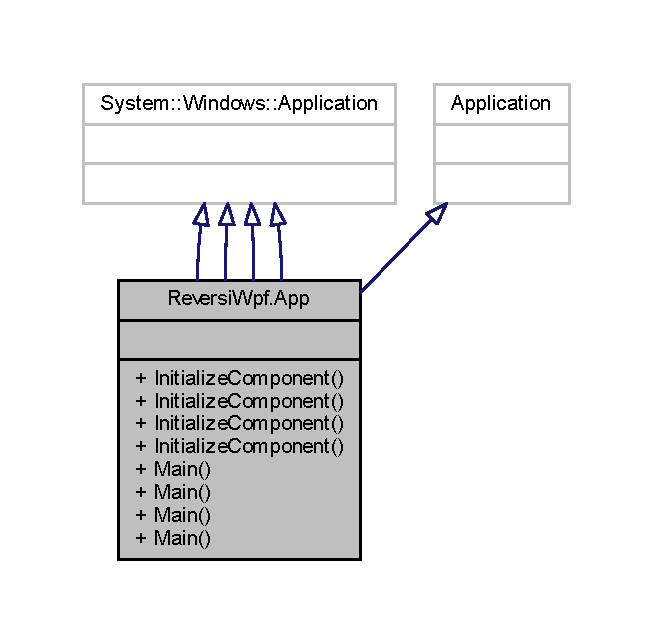
\includegraphics[width=314pt]{class_reversi_wpf_1_1_app__inherit__graph}
\end{center}
\end{figure}


Collaboration diagram for Reversi\+Wpf.\+App\+:\nopagebreak
\begin{figure}[H]
\begin{center}
\leavevmode
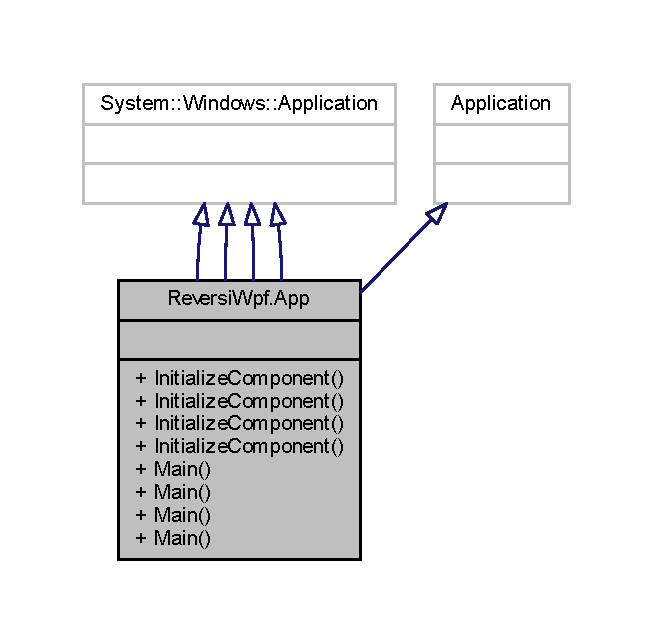
\includegraphics[width=314pt]{class_reversi_wpf_1_1_app__coll__graph}
\end{center}
\end{figure}
\subsection*{Public Member Functions}
\begin{DoxyCompactItemize}
\item 
void \hyperlink{class_reversi_wpf_1_1_app_a30ccf063a596c89bd03747d60a96d084}{Initialize\+Component} ()
\begin{DoxyCompactList}\small\item\em Initialize\+Component \end{DoxyCompactList}\item 
void \hyperlink{class_reversi_wpf_1_1_app_a30ccf063a596c89bd03747d60a96d084}{Initialize\+Component} ()
\begin{DoxyCompactList}\small\item\em Initialize\+Component \end{DoxyCompactList}\item 
void \hyperlink{class_reversi_wpf_1_1_app_a30ccf063a596c89bd03747d60a96d084}{Initialize\+Component} ()
\begin{DoxyCompactList}\small\item\em Initialize\+Component \end{DoxyCompactList}\item 
void \hyperlink{class_reversi_wpf_1_1_app_a30ccf063a596c89bd03747d60a96d084}{Initialize\+Component} ()
\begin{DoxyCompactList}\small\item\em Initialize\+Component \end{DoxyCompactList}\end{DoxyCompactItemize}
\subsection*{Static Public Member Functions}
\begin{DoxyCompactItemize}
\item 
static void \hyperlink{class_reversi_wpf_1_1_app_a21f38c0f40a47a04302edeeb7bf005f8}{Main} ()
\begin{DoxyCompactList}\small\item\em Application Entry Point. \end{DoxyCompactList}\item 
static void \hyperlink{class_reversi_wpf_1_1_app_a21f38c0f40a47a04302edeeb7bf005f8}{Main} ()
\begin{DoxyCompactList}\small\item\em Application Entry Point. \end{DoxyCompactList}\item 
static void \hyperlink{class_reversi_wpf_1_1_app_a21f38c0f40a47a04302edeeb7bf005f8}{Main} ()
\begin{DoxyCompactList}\small\item\em Application Entry Point. \end{DoxyCompactList}\item 
static void \hyperlink{class_reversi_wpf_1_1_app_a21f38c0f40a47a04302edeeb7bf005f8}{Main} ()
\begin{DoxyCompactList}\small\item\em Application Entry Point. \end{DoxyCompactList}\end{DoxyCompactItemize}


\subsection{Detailed Description}
App.\+xaml の相互作用ロジック 

\hyperlink{class_reversi_wpf_1_1_app}{App} 

Definition at line 14 of file App.\+xaml.\+cs.



\subsection{Member Function Documentation}
\mbox{\Hypertarget{class_reversi_wpf_1_1_app_a30ccf063a596c89bd03747d60a96d084}\label{class_reversi_wpf_1_1_app_a30ccf063a596c89bd03747d60a96d084}} 
\index{Reversi\+Wpf\+::\+App@{Reversi\+Wpf\+::\+App}!Initialize\+Component@{Initialize\+Component}}
\index{Initialize\+Component@{Initialize\+Component}!Reversi\+Wpf\+::\+App@{Reversi\+Wpf\+::\+App}}
\subsubsection{\texorpdfstring{Initialize\+Component()}{InitializeComponent()}\hspace{0.1cm}{\footnotesize\ttfamily [1/4]}}
{\footnotesize\ttfamily void Reversi\+Wpf.\+App.\+Initialize\+Component (\begin{DoxyParamCaption}{ }\end{DoxyParamCaption})}



Initialize\+Component 



Definition at line 48 of file App.\+g.\+cs.



Referenced by Reversi\+Wpf.\+App.\+Main().

Here is the caller graph for this function\+:\nopagebreak
\begin{figure}[H]
\begin{center}
\leavevmode
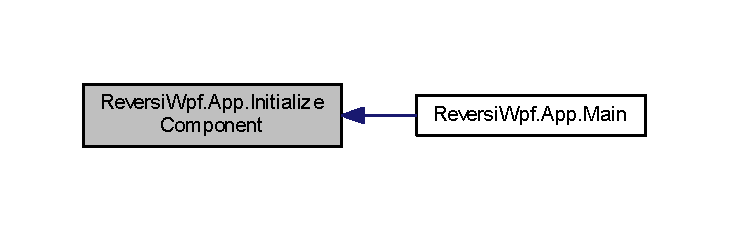
\includegraphics[width=350pt]{class_reversi_wpf_1_1_app_a30ccf063a596c89bd03747d60a96d084_icgraph}
\end{center}
\end{figure}
\mbox{\Hypertarget{class_reversi_wpf_1_1_app_a30ccf063a596c89bd03747d60a96d084}\label{class_reversi_wpf_1_1_app_a30ccf063a596c89bd03747d60a96d084}} 
\index{Reversi\+Wpf\+::\+App@{Reversi\+Wpf\+::\+App}!Initialize\+Component@{Initialize\+Component}}
\index{Initialize\+Component@{Initialize\+Component}!Reversi\+Wpf\+::\+App@{Reversi\+Wpf\+::\+App}}
\subsubsection{\texorpdfstring{Initialize\+Component()}{InitializeComponent()}\hspace{0.1cm}{\footnotesize\ttfamily [2/4]}}
{\footnotesize\ttfamily void Reversi\+Wpf.\+App.\+Initialize\+Component (\begin{DoxyParamCaption}{ }\end{DoxyParamCaption})}



Initialize\+Component 



Definition at line 48 of file App.\+g.\+cs.

\mbox{\Hypertarget{class_reversi_wpf_1_1_app_a30ccf063a596c89bd03747d60a96d084}\label{class_reversi_wpf_1_1_app_a30ccf063a596c89bd03747d60a96d084}} 
\index{Reversi\+Wpf\+::\+App@{Reversi\+Wpf\+::\+App}!Initialize\+Component@{Initialize\+Component}}
\index{Initialize\+Component@{Initialize\+Component}!Reversi\+Wpf\+::\+App@{Reversi\+Wpf\+::\+App}}
\subsubsection{\texorpdfstring{Initialize\+Component()}{InitializeComponent()}\hspace{0.1cm}{\footnotesize\ttfamily [3/4]}}
{\footnotesize\ttfamily void Reversi\+Wpf.\+App.\+Initialize\+Component (\begin{DoxyParamCaption}{ }\end{DoxyParamCaption})}



Initialize\+Component 



Definition at line 48 of file App.\+g.\+i.\+cs.

\mbox{\Hypertarget{class_reversi_wpf_1_1_app_a30ccf063a596c89bd03747d60a96d084}\label{class_reversi_wpf_1_1_app_a30ccf063a596c89bd03747d60a96d084}} 
\index{Reversi\+Wpf\+::\+App@{Reversi\+Wpf\+::\+App}!Initialize\+Component@{Initialize\+Component}}
\index{Initialize\+Component@{Initialize\+Component}!Reversi\+Wpf\+::\+App@{Reversi\+Wpf\+::\+App}}
\subsubsection{\texorpdfstring{Initialize\+Component()}{InitializeComponent()}\hspace{0.1cm}{\footnotesize\ttfamily [4/4]}}
{\footnotesize\ttfamily void Reversi\+Wpf.\+App.\+Initialize\+Component (\begin{DoxyParamCaption}{ }\end{DoxyParamCaption})}



Initialize\+Component 



Definition at line 48 of file App.\+g.\+i.\+cs.

\mbox{\Hypertarget{class_reversi_wpf_1_1_app_a21f38c0f40a47a04302edeeb7bf005f8}\label{class_reversi_wpf_1_1_app_a21f38c0f40a47a04302edeeb7bf005f8}} 
\index{Reversi\+Wpf\+::\+App@{Reversi\+Wpf\+::\+App}!Main@{Main}}
\index{Main@{Main}!Reversi\+Wpf\+::\+App@{Reversi\+Wpf\+::\+App}}
\subsubsection{\texorpdfstring{Main()}{Main()}\hspace{0.1cm}{\footnotesize\ttfamily [1/4]}}
{\footnotesize\ttfamily static void Reversi\+Wpf.\+App.\+Main (\begin{DoxyParamCaption}{ }\end{DoxyParamCaption})\hspace{0.3cm}{\ttfamily [static]}}



Application Entry Point. 



Definition at line 63 of file App.\+g.\+cs.

Here is the call graph for this function\+:
\nopagebreak
\begin{figure}[H]
\begin{center}
\leavevmode
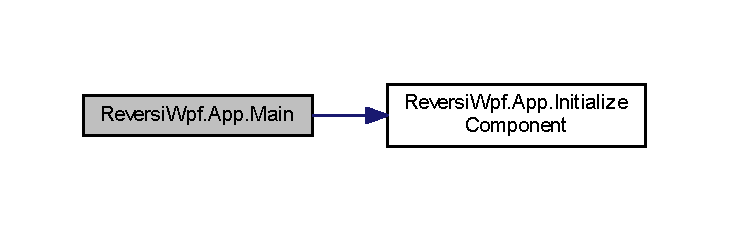
\includegraphics[width=350pt]{class_reversi_wpf_1_1_app_a21f38c0f40a47a04302edeeb7bf005f8_cgraph}
\end{center}
\end{figure}
\mbox{\Hypertarget{class_reversi_wpf_1_1_app_a21f38c0f40a47a04302edeeb7bf005f8}\label{class_reversi_wpf_1_1_app_a21f38c0f40a47a04302edeeb7bf005f8}} 
\index{Reversi\+Wpf\+::\+App@{Reversi\+Wpf\+::\+App}!Main@{Main}}
\index{Main@{Main}!Reversi\+Wpf\+::\+App@{Reversi\+Wpf\+::\+App}}
\subsubsection{\texorpdfstring{Main()}{Main()}\hspace{0.1cm}{\footnotesize\ttfamily [2/4]}}
{\footnotesize\ttfamily static void Reversi\+Wpf.\+App.\+Main (\begin{DoxyParamCaption}{ }\end{DoxyParamCaption})\hspace{0.3cm}{\ttfamily [static]}}



Application Entry Point. 



Definition at line 63 of file App.\+g.\+i.\+cs.

Here is the call graph for this function\+:
\nopagebreak
\begin{figure}[H]
\begin{center}
\leavevmode
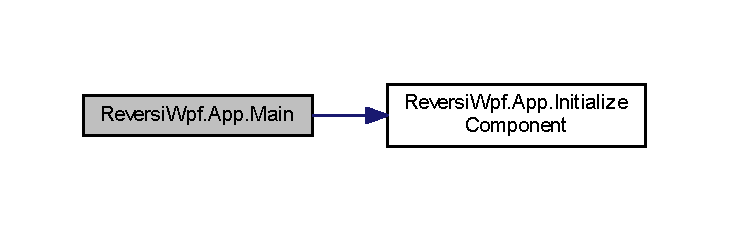
\includegraphics[width=350pt]{class_reversi_wpf_1_1_app_a21f38c0f40a47a04302edeeb7bf005f8_cgraph}
\end{center}
\end{figure}
\mbox{\Hypertarget{class_reversi_wpf_1_1_app_a21f38c0f40a47a04302edeeb7bf005f8}\label{class_reversi_wpf_1_1_app_a21f38c0f40a47a04302edeeb7bf005f8}} 
\index{Reversi\+Wpf\+::\+App@{Reversi\+Wpf\+::\+App}!Main@{Main}}
\index{Main@{Main}!Reversi\+Wpf\+::\+App@{Reversi\+Wpf\+::\+App}}
\subsubsection{\texorpdfstring{Main()}{Main()}\hspace{0.1cm}{\footnotesize\ttfamily [3/4]}}
{\footnotesize\ttfamily static void Reversi\+Wpf.\+App.\+Main (\begin{DoxyParamCaption}{ }\end{DoxyParamCaption})\hspace{0.3cm}{\ttfamily [static]}}



Application Entry Point. 



Definition at line 63 of file App.\+g.\+cs.

Here is the call graph for this function\+:
\nopagebreak
\begin{figure}[H]
\begin{center}
\leavevmode
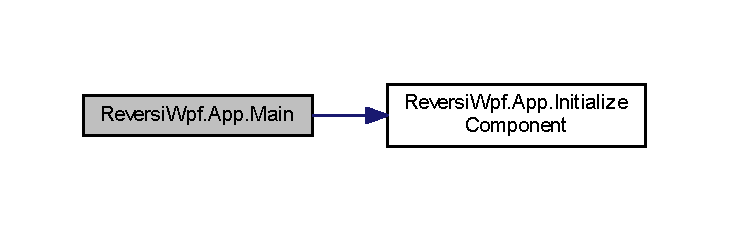
\includegraphics[width=350pt]{class_reversi_wpf_1_1_app_a21f38c0f40a47a04302edeeb7bf005f8_cgraph}
\end{center}
\end{figure}
\mbox{\Hypertarget{class_reversi_wpf_1_1_app_a21f38c0f40a47a04302edeeb7bf005f8}\label{class_reversi_wpf_1_1_app_a21f38c0f40a47a04302edeeb7bf005f8}} 
\index{Reversi\+Wpf\+::\+App@{Reversi\+Wpf\+::\+App}!Main@{Main}}
\index{Main@{Main}!Reversi\+Wpf\+::\+App@{Reversi\+Wpf\+::\+App}}
\subsubsection{\texorpdfstring{Main()}{Main()}\hspace{0.1cm}{\footnotesize\ttfamily [4/4]}}
{\footnotesize\ttfamily static void Reversi\+Wpf.\+App.\+Main (\begin{DoxyParamCaption}{ }\end{DoxyParamCaption})\hspace{0.3cm}{\ttfamily [static]}}



Application Entry Point. 



Definition at line 63 of file App.\+g.\+i.\+cs.

Here is the call graph for this function\+:
\nopagebreak
\begin{figure}[H]
\begin{center}
\leavevmode
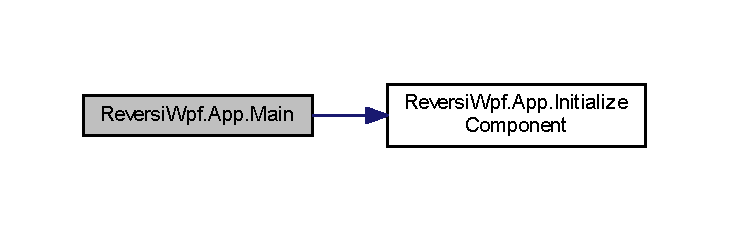
\includegraphics[width=350pt]{class_reversi_wpf_1_1_app_a21f38c0f40a47a04302edeeb7bf005f8_cgraph}
\end{center}
\end{figure}


The documentation for this class was generated from the following files\+:\begin{DoxyCompactItemize}
\item 
App.\+xaml.\+cs\item 
obj/\+Debug/App.\+g.\+cs\item 
obj/\+Debug/App.\+g.\+i.\+cs\end{DoxyCompactItemize}

\hypertarget{class_reversi_wpf_1_1_hsl_color}{}\section{Reversi\+Wpf.\+Hsl\+Color Class Reference}
\label{class_reversi_wpf_1_1_hsl_color}\index{Reversi\+Wpf.\+Hsl\+Color@{Reversi\+Wpf.\+Hsl\+Color}}


H\+SL (H\+LS) カラーを表す  




Collaboration diagram for Reversi\+Wpf.\+Hsl\+Color\+:
\nopagebreak
\begin{figure}[H]
\begin{center}
\leavevmode
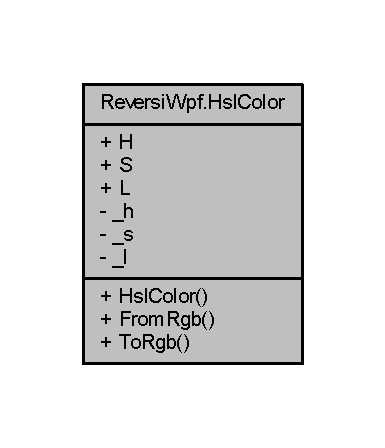
\includegraphics[width=185pt]{class_reversi_wpf_1_1_hsl_color__coll__graph}
\end{center}
\end{figure}
\subsection*{Public Member Functions}
\begin{DoxyCompactItemize}
\item 
\mbox{\Hypertarget{class_reversi_wpf_1_1_hsl_color_a55ebdc383bf75f88cc61e6312f8899ba}\label{class_reversi_wpf_1_1_hsl_color_a55ebdc383bf75f88cc61e6312f8899ba}} 
{\bfseries Hsl\+Color} (float hue, float saturation, float lightness)
\end{DoxyCompactItemize}
\subsection*{Static Public Member Functions}
\begin{DoxyCompactItemize}
\item 
static \hyperlink{class_reversi_wpf_1_1_hsl_color}{Hsl\+Color} \hyperlink{class_reversi_wpf_1_1_hsl_color_a0725f254d6e13cd9e7114fe8b1645954}{From\+Rgb} (Color rgb)
\begin{DoxyCompactList}\small\item\em 指定した\+Colorから\+Hsl\+Colorを作成する \end{DoxyCompactList}\item 
static Color \hyperlink{class_reversi_wpf_1_1_hsl_color_aba11bae61cc67fcece49cbc4b18db8b1}{To\+Rgb} (\hyperlink{class_reversi_wpf_1_1_hsl_color}{Hsl\+Color} hsl)
\begin{DoxyCompactList}\small\item\em 指定した\+Hsl\+Colorから\+Colorを作成する \end{DoxyCompactList}\end{DoxyCompactItemize}
\subsection*{Properties}
\begin{DoxyCompactItemize}
\item 
float \hyperlink{class_reversi_wpf_1_1_hsl_color_a8b56c1b47fa4880e598829435ca25122}{H}\hspace{0.3cm}{\ttfamily  \mbox{[}get\mbox{]}}
\begin{DoxyCompactList}\small\item\em 色相 (Hue) \end{DoxyCompactList}\item 
float \hyperlink{class_reversi_wpf_1_1_hsl_color_a3304ba59ade02e6ad5ced23120e72bdc}{S}\hspace{0.3cm}{\ttfamily  \mbox{[}get\mbox{]}}
\begin{DoxyCompactList}\small\item\em 彩度 (Saturation) \end{DoxyCompactList}\item 
float \hyperlink{class_reversi_wpf_1_1_hsl_color_a8d465b3c48d716f819d8a53a4eca3d93}{L}\hspace{0.3cm}{\ttfamily  \mbox{[}get\mbox{]}}
\begin{DoxyCompactList}\small\item\em 輝度 (Lightness) \end{DoxyCompactList}\end{DoxyCompactItemize}
\subsection*{Private Attributes}
\begin{DoxyCompactItemize}
\item 
\mbox{\Hypertarget{class_reversi_wpf_1_1_hsl_color_a0ab31c8cfeea24ffb4a8a5dfcc7dd817}\label{class_reversi_wpf_1_1_hsl_color_a0ab31c8cfeea24ffb4a8a5dfcc7dd817}} 
float {\bfseries \+\_\+h}
\item 
\mbox{\Hypertarget{class_reversi_wpf_1_1_hsl_color_a421d055ca374af31bc7153f0103bba72}\label{class_reversi_wpf_1_1_hsl_color_a421d055ca374af31bc7153f0103bba72}} 
float {\bfseries \+\_\+s}
\item 
\mbox{\Hypertarget{class_reversi_wpf_1_1_hsl_color_ad8e0aa4c03ad37fdff47d2808c70a184}\label{class_reversi_wpf_1_1_hsl_color_ad8e0aa4c03ad37fdff47d2808c70a184}} 
float {\bfseries \+\_\+l}
\end{DoxyCompactItemize}


\subsection{Detailed Description}
H\+SL (H\+LS) カラーを表す 

Definition at line 28 of file Hsl\+Color.\+cs.



\subsection{Member Function Documentation}
\mbox{\Hypertarget{class_reversi_wpf_1_1_hsl_color_a0725f254d6e13cd9e7114fe8b1645954}\label{class_reversi_wpf_1_1_hsl_color_a0725f254d6e13cd9e7114fe8b1645954}} 
\index{Reversi\+Wpf\+::\+Hsl\+Color@{Reversi\+Wpf\+::\+Hsl\+Color}!From\+Rgb@{From\+Rgb}}
\index{From\+Rgb@{From\+Rgb}!Reversi\+Wpf\+::\+Hsl\+Color@{Reversi\+Wpf\+::\+Hsl\+Color}}
\subsubsection{\texorpdfstring{From\+Rgb()}{FromRgb()}}
{\footnotesize\ttfamily static \hyperlink{class_reversi_wpf_1_1_hsl_color}{Hsl\+Color} Reversi\+Wpf.\+Hsl\+Color.\+From\+Rgb (\begin{DoxyParamCaption}\item[{Color}]{rgb }\end{DoxyParamCaption})\hspace{0.3cm}{\ttfamily [static]}}



指定した\+Colorから\+Hsl\+Colorを作成する 


\begin{DoxyParams}{Parameters}
{\em rgb} & Color\\
\hline
\end{DoxyParams}
\begin{DoxyReturn}{Returns}
\hyperlink{class_reversi_wpf_1_1_hsl_color}{Hsl\+Color}
\end{DoxyReturn}


Definition at line 82 of file Hsl\+Color.\+cs.



Referenced by Reversi\+Wpf.\+Main\+Window.\+Draw\+Single\+Local().

Here is the caller graph for this function\+:
\nopagebreak
\begin{figure}[H]
\begin{center}
\leavevmode
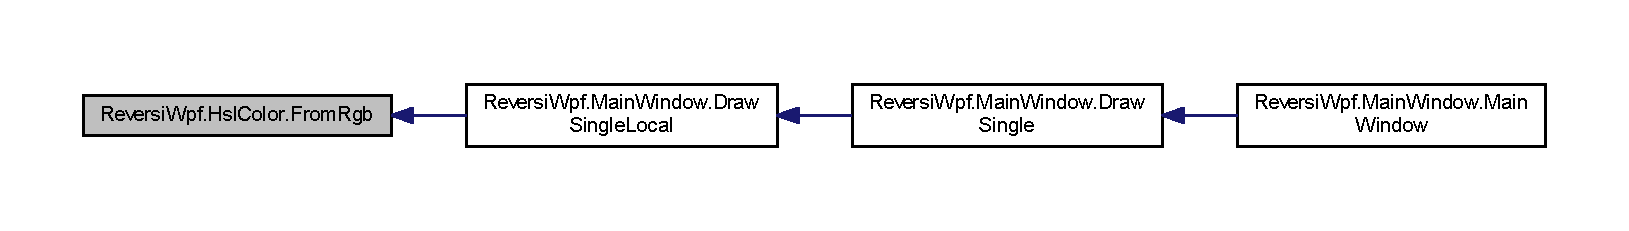
\includegraphics[width=350pt]{class_reversi_wpf_1_1_hsl_color_a0725f254d6e13cd9e7114fe8b1645954_icgraph}
\end{center}
\end{figure}
\mbox{\Hypertarget{class_reversi_wpf_1_1_hsl_color_aba11bae61cc67fcece49cbc4b18db8b1}\label{class_reversi_wpf_1_1_hsl_color_aba11bae61cc67fcece49cbc4b18db8b1}} 
\index{Reversi\+Wpf\+::\+Hsl\+Color@{Reversi\+Wpf\+::\+Hsl\+Color}!To\+Rgb@{To\+Rgb}}
\index{To\+Rgb@{To\+Rgb}!Reversi\+Wpf\+::\+Hsl\+Color@{Reversi\+Wpf\+::\+Hsl\+Color}}
\subsubsection{\texorpdfstring{To\+Rgb()}{ToRgb()}}
{\footnotesize\ttfamily static Color Reversi\+Wpf.\+Hsl\+Color.\+To\+Rgb (\begin{DoxyParamCaption}\item[{\hyperlink{class_reversi_wpf_1_1_hsl_color}{Hsl\+Color}}]{hsl }\end{DoxyParamCaption})\hspace{0.3cm}{\ttfamily [static]}}



指定した\+Hsl\+Colorから\+Colorを作成する 


\begin{DoxyParams}{Parameters}
{\em hsl} & \hyperlink{class_reversi_wpf_1_1_hsl_color}{Hsl\+Color}\\
\hline
\end{DoxyParams}
\begin{DoxyReturn}{Returns}
Color
\end{DoxyReturn}


Definition at line 141 of file Hsl\+Color.\+cs.



Referenced by Reversi\+Wpf.\+Main\+Window.\+Draw\+Single\+Local().

Here is the caller graph for this function\+:
\nopagebreak
\begin{figure}[H]
\begin{center}
\leavevmode
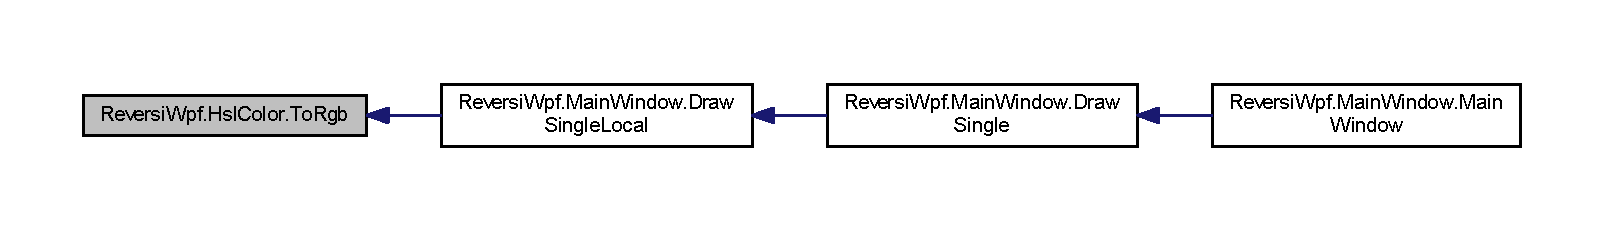
\includegraphics[width=350pt]{class_reversi_wpf_1_1_hsl_color_aba11bae61cc67fcece49cbc4b18db8b1_icgraph}
\end{center}
\end{figure}


\subsection{Property Documentation}
\mbox{\Hypertarget{class_reversi_wpf_1_1_hsl_color_a8b56c1b47fa4880e598829435ca25122}\label{class_reversi_wpf_1_1_hsl_color_a8b56c1b47fa4880e598829435ca25122}} 
\index{Reversi\+Wpf\+::\+Hsl\+Color@{Reversi\+Wpf\+::\+Hsl\+Color}!H@{H}}
\index{H@{H}!Reversi\+Wpf\+::\+Hsl\+Color@{Reversi\+Wpf\+::\+Hsl\+Color}}
\subsubsection{\texorpdfstring{H}{H}}
{\footnotesize\ttfamily float Reversi\+Wpf.\+Hsl\+Color.\+H\hspace{0.3cm}{\ttfamily [get]}}



色相 (Hue) 



Definition at line 35 of file Hsl\+Color.\+cs.



Referenced by Reversi\+Wpf.\+Main\+Window.\+Draw\+Single\+Local(), and Reversi\+Wpf.\+Hsl\+Color.\+To\+Rgb().

\mbox{\Hypertarget{class_reversi_wpf_1_1_hsl_color_a8d465b3c48d716f819d8a53a4eca3d93}\label{class_reversi_wpf_1_1_hsl_color_a8d465b3c48d716f819d8a53a4eca3d93}} 
\index{Reversi\+Wpf\+::\+Hsl\+Color@{Reversi\+Wpf\+::\+Hsl\+Color}!L@{L}}
\index{L@{L}!Reversi\+Wpf\+::\+Hsl\+Color@{Reversi\+Wpf\+::\+Hsl\+Color}}
\subsubsection{\texorpdfstring{L}{L}}
{\footnotesize\ttfamily float Reversi\+Wpf.\+Hsl\+Color.\+L\hspace{0.3cm}{\ttfamily [get]}}



輝度 (Lightness) 



Definition at line 53 of file Hsl\+Color.\+cs.



Referenced by Reversi\+Wpf.\+Main\+Window.\+Draw\+Single\+Local(), and Reversi\+Wpf.\+Hsl\+Color.\+To\+Rgb().

\mbox{\Hypertarget{class_reversi_wpf_1_1_hsl_color_a3304ba59ade02e6ad5ced23120e72bdc}\label{class_reversi_wpf_1_1_hsl_color_a3304ba59ade02e6ad5ced23120e72bdc}} 
\index{Reversi\+Wpf\+::\+Hsl\+Color@{Reversi\+Wpf\+::\+Hsl\+Color}!S@{S}}
\index{S@{S}!Reversi\+Wpf\+::\+Hsl\+Color@{Reversi\+Wpf\+::\+Hsl\+Color}}
\subsubsection{\texorpdfstring{S}{S}}
{\footnotesize\ttfamily float Reversi\+Wpf.\+Hsl\+Color.\+S\hspace{0.3cm}{\ttfamily [get]}}



彩度 (Saturation) 



Definition at line 44 of file Hsl\+Color.\+cs.



Referenced by Reversi\+Wpf.\+Main\+Window.\+Draw\+Single\+Local(), and Reversi\+Wpf.\+Hsl\+Color.\+To\+Rgb().



The documentation for this class was generated from the following file\+:\begin{DoxyCompactItemize}
\item 
Model/\hyperlink{_hsl_color_8cs}{Hsl\+Color.\+cs}\end{DoxyCompactItemize}

\hypertarget{class_reversi_wpf_1_1_main_window}{}\section{Reversi\+Wpf.\+Main\+Window Class Reference}
\label{class_reversi_wpf_1_1_main_window}\index{Reversi\+Wpf.\+Main\+Window@{Reversi\+Wpf.\+Main\+Window}}


\hyperlink{class_reversi_wpf_1_1_main_window}{Main\+Window}  




Inheritance diagram for Reversi\+Wpf.\+Main\+Window\+:
\nopagebreak
\begin{figure}[H]
\begin{center}
\leavevmode
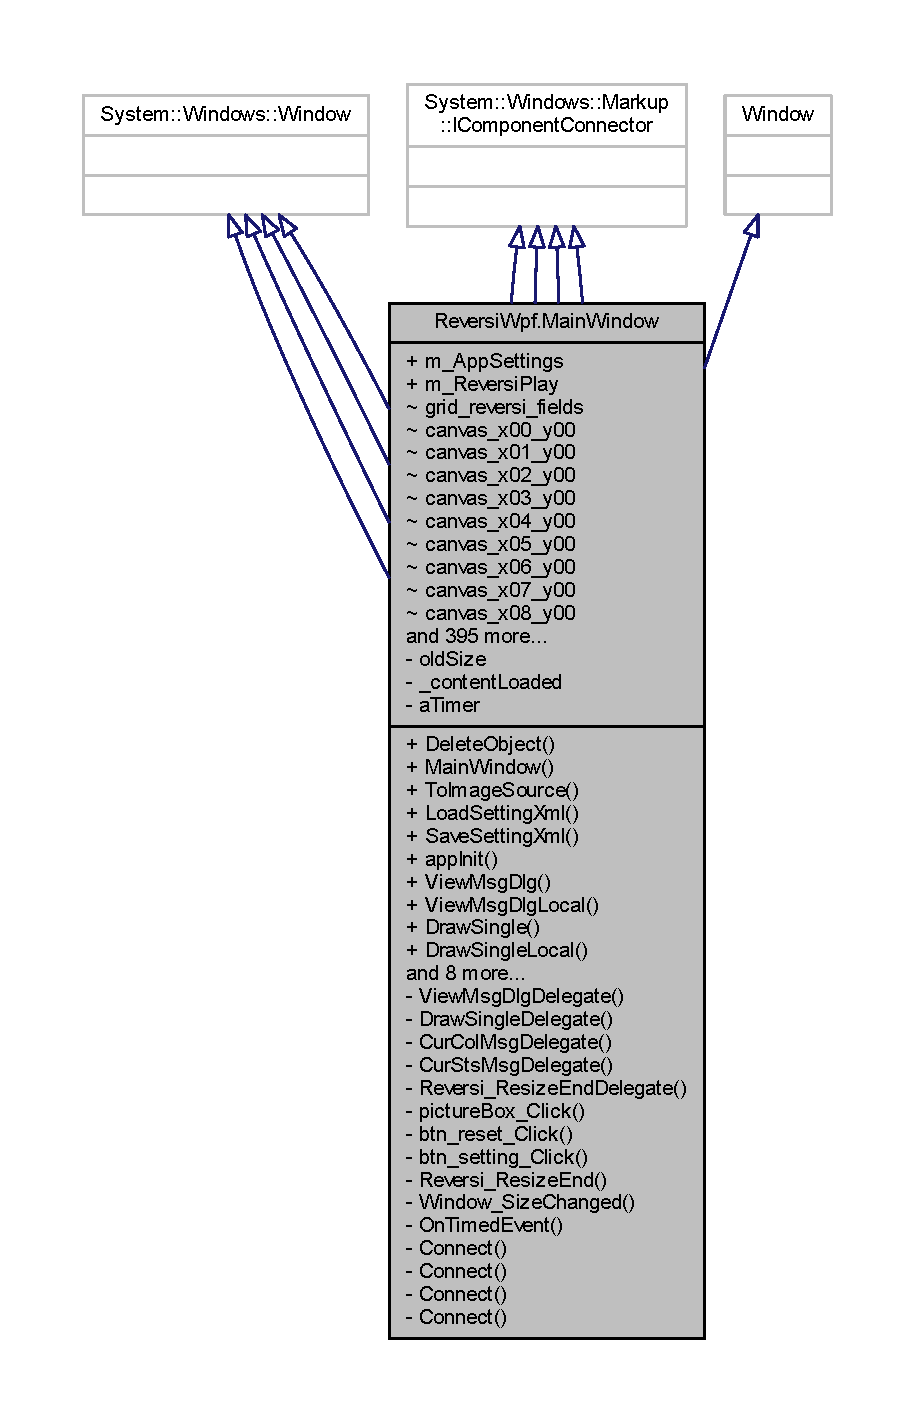
\includegraphics[width=350pt]{class_reversi_wpf_1_1_main_window__inherit__graph}
\end{center}
\end{figure}


Collaboration diagram for Reversi\+Wpf.\+Main\+Window\+:
\nopagebreak
\begin{figure}[H]
\begin{center}
\leavevmode
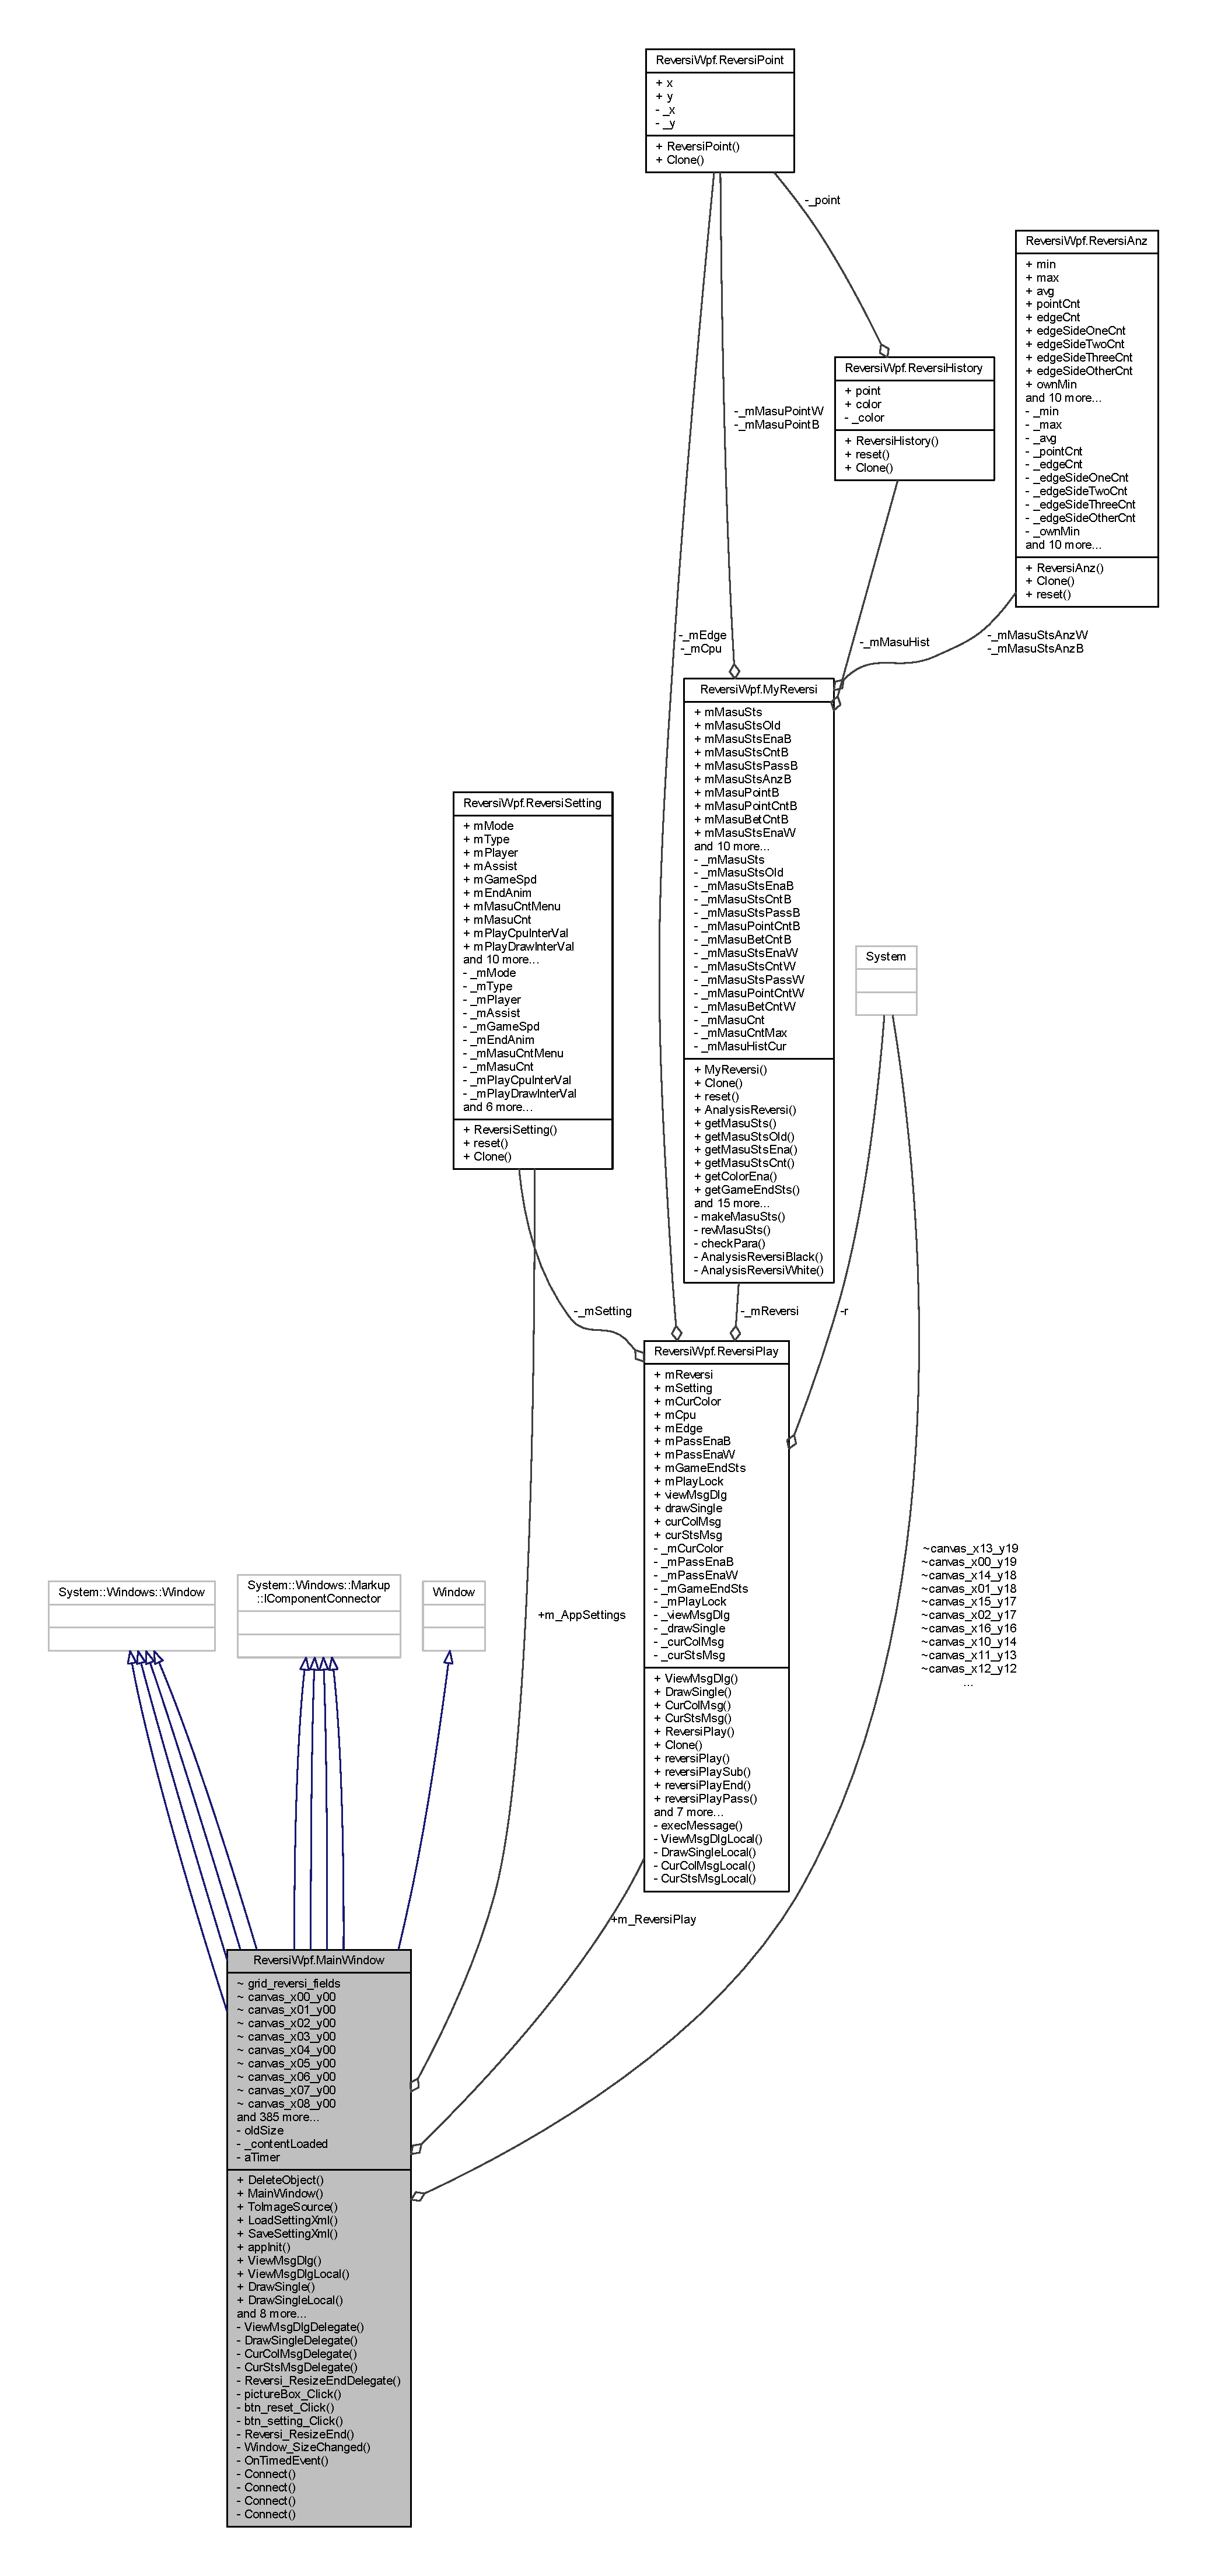
\includegraphics[height=550pt]{class_reversi_wpf_1_1_main_window__coll__graph}
\end{center}
\end{figure}
\subsection*{Public Member Functions}
\begin{DoxyCompactItemize}
\item 
\mbox{\Hypertarget{class_reversi_wpf_1_1_main_window_a304cbdac5bcab90066c84c1e6b9b0856}\label{class_reversi_wpf_1_1_main_window_a304cbdac5bcab90066c84c1e6b9b0856}} 
static bool \hyperlink{class_reversi_wpf_1_1_main_window_a304cbdac5bcab90066c84c1e6b9b0856}{Delete\+Object} (Int\+Ptr h\+Object)
\begin{DoxyCompactList}\small\item\em gdi32.\+dllの\+Delete\+Objectメソッドの使用を宣言する。 \end{DoxyCompactList}\item 
\hyperlink{class_reversi_wpf_1_1_main_window_af64ecb3857a3d547b4020e9900048360}{Main\+Window} ()
\begin{DoxyCompactList}\small\item\em コンストラクタ \end{DoxyCompactList}\item 
Image\+Source \hyperlink{class_reversi_wpf_1_1_main_window_a5c093af07e7e92f21127941dff8e8684}{To\+Image\+Source} (Bitmap bmp)
\begin{DoxyCompactList}\small\item\em B\+I\+T\+M\+A\+Pか\+Image\+Sourceに変換 \end{DoxyCompactList}\item 
\hyperlink{class_reversi_wpf_1_1_reversi_setting}{Reversi\+Setting} \hyperlink{class_reversi_wpf_1_1_main_window_ad911eb50aa81ec46e9f1032f264ee483}{Load\+Setting\+Xml} (string path)
\begin{DoxyCompactList}\small\item\em 設定\+X\+M\+Lファイルロード \end{DoxyCompactList}\item 
int \hyperlink{class_reversi_wpf_1_1_main_window_a02e0ae28907a572eca49167b37ce7db9}{Save\+Setting\+Xml} (string path, ref \hyperlink{class_reversi_wpf_1_1_reversi_setting}{Reversi\+Setting} app\+Set)
\begin{DoxyCompactList}\small\item\em 設定\+X\+M\+Lファイルセーブ \end{DoxyCompactList}\item 
void \hyperlink{class_reversi_wpf_1_1_main_window_a4e9c1014738c9b72f093dbc179ce984e}{app\+Init} ()
\begin{DoxyCompactList}\small\item\em アプリ初期化 \end{DoxyCompactList}\item 
void \hyperlink{class_reversi_wpf_1_1_main_window_aa776c697ed89869c9799576f2f6022b9}{View\+Msg\+Dlg} (string title, string msg)
\begin{DoxyCompactList}\small\item\em メッセージダイアログ \end{DoxyCompactList}\item 
void \hyperlink{class_reversi_wpf_1_1_main_window_a3095c98dbf6fcd1f738354a06797beb1}{View\+Msg\+Dlg\+Local} (string title, string msg)
\begin{DoxyCompactList}\small\item\em メッセージダイアログ \end{DoxyCompactList}\item 
void \hyperlink{class_reversi_wpf_1_1_main_window_aa7f29f9037ca59f0b41d4b383875bb5e}{Draw\+Single} (int y, int x, int sts, int bk, string text)
\begin{DoxyCompactList}\small\item\em 1マス描画 \end{DoxyCompactList}\item 
void \hyperlink{class_reversi_wpf_1_1_main_window_a88fd4a18ce06e08801a3370147bc3a8b}{Draw\+Single\+Local} (int y, int x, int sts, int bk, string text)
\begin{DoxyCompactList}\small\item\em 1マス描画 \end{DoxyCompactList}\item 
void \hyperlink{class_reversi_wpf_1_1_main_window_a5dd2bbfd5f17c36d1b301fdb91b483ad}{Cur\+Col\+Msg} (string text)
\begin{DoxyCompactList}\small\item\em 現在の色メッセージ \end{DoxyCompactList}\item 
void \hyperlink{class_reversi_wpf_1_1_main_window_a92d45fe8b0224e36ce974e04388ec541}{Cur\+Col\+Msg\+Local} (string text)
\begin{DoxyCompactList}\small\item\em 現在の色メッセージ \end{DoxyCompactList}\item 
void \hyperlink{class_reversi_wpf_1_1_main_window_a90e6aa75849526159fe9348da2b66fb0}{Cur\+Sts\+Msg} (string text)
\begin{DoxyCompactList}\small\item\em 現在のステータスメッセージ \end{DoxyCompactList}\item 
void \hyperlink{class_reversi_wpf_1_1_main_window_a73402ffecf2de584339327dce357bd60}{Cur\+Sts\+Msg\+Local} (string text)
\begin{DoxyCompactList}\small\item\em 現在のステータスメッセージ \end{DoxyCompactList}\item 
void \hyperlink{class_reversi_wpf_1_1_main_window_a4cf9bc92cee02fa8e3b00fa56fb41c82}{Initialize\+Component} ()
\begin{DoxyCompactList}\small\item\em Initialize\+Component \end{DoxyCompactList}\item 
void \hyperlink{class_reversi_wpf_1_1_main_window_a4cf9bc92cee02fa8e3b00fa56fb41c82}{Initialize\+Component} ()
\begin{DoxyCompactList}\small\item\em Initialize\+Component \end{DoxyCompactList}\item 
void \hyperlink{class_reversi_wpf_1_1_main_window_a4cf9bc92cee02fa8e3b00fa56fb41c82}{Initialize\+Component} ()
\begin{DoxyCompactList}\small\item\em Initialize\+Component \end{DoxyCompactList}\item 
void \hyperlink{class_reversi_wpf_1_1_main_window_a4cf9bc92cee02fa8e3b00fa56fb41c82}{Initialize\+Component} ()
\begin{DoxyCompactList}\small\item\em Initialize\+Component \end{DoxyCompactList}\end{DoxyCompactItemize}
\subsection*{Public Attributes}
\begin{DoxyCompactItemize}
\item 
\mbox{\Hypertarget{class_reversi_wpf_1_1_main_window_a8c1c460437b8e632cb9666a71a8ecbdb}\label{class_reversi_wpf_1_1_main_window_a8c1c460437b8e632cb9666a71a8ecbdb}} 
\hyperlink{class_reversi_wpf_1_1_reversi_setting}{Reversi\+Setting} \hyperlink{class_reversi_wpf_1_1_main_window_a8c1c460437b8e632cb9666a71a8ecbdb}{m\+\_\+\+App\+Settings}
\begin{DoxyCompactList}\small\item\em アプリ設定 \end{DoxyCompactList}\item 
\mbox{\Hypertarget{class_reversi_wpf_1_1_main_window_a1722c45ebaa15e7ea8f895946516771e}\label{class_reversi_wpf_1_1_main_window_a1722c45ebaa15e7ea8f895946516771e}} 
\hyperlink{class_reversi_wpf_1_1_reversi_play}{Reversi\+Play} \hyperlink{class_reversi_wpf_1_1_main_window_a1722c45ebaa15e7ea8f895946516771e}{m\+\_\+\+Reversi\+Play}
\begin{DoxyCompactList}\small\item\em リバーシ本体 \end{DoxyCompactList}\end{DoxyCompactItemize}
\subsection*{Private Member Functions}
\begin{DoxyCompactItemize}
\item 
\mbox{\Hypertarget{class_reversi_wpf_1_1_main_window_a0e8395f8250557e220e7991b1ab35f75}\label{class_reversi_wpf_1_1_main_window_a0e8395f8250557e220e7991b1ab35f75}} 
delegate void {\bfseries View\+Msg\+Dlg\+Delegate} (string title, string msg)
\item 
\mbox{\Hypertarget{class_reversi_wpf_1_1_main_window_a65ef9ec2bd0530c4174e5400417ba502}\label{class_reversi_wpf_1_1_main_window_a65ef9ec2bd0530c4174e5400417ba502}} 
delegate void {\bfseries Draw\+Single\+Delegate} (int y, int x, int sts, int bk, string text)
\item 
\mbox{\Hypertarget{class_reversi_wpf_1_1_main_window_ae65f508538317670624e86938d8f97ac}\label{class_reversi_wpf_1_1_main_window_ae65f508538317670624e86938d8f97ac}} 
delegate void {\bfseries Cur\+Col\+Msg\+Delegate} (string text)
\item 
\mbox{\Hypertarget{class_reversi_wpf_1_1_main_window_a42bb52b7954bd84a3d739975db7c2779}\label{class_reversi_wpf_1_1_main_window_a42bb52b7954bd84a3d739975db7c2779}} 
delegate void {\bfseries Cur\+Sts\+Msg\+Delegate} (string text)
\item 
\mbox{\Hypertarget{class_reversi_wpf_1_1_main_window_acd320193924986ad56929164d8a8d167}\label{class_reversi_wpf_1_1_main_window_acd320193924986ad56929164d8a8d167}} 
delegate void {\bfseries Reversi\+\_\+\+Resize\+End\+Delegate} (object sender, Event\+Args e)
\item 
void \hyperlink{class_reversi_wpf_1_1_main_window_a7514a29baed5a572e78354addb9678bc}{picture\+Box\+\_\+\+Click} (object sender, Mouse\+Button\+Event\+Args e)
\begin{DoxyCompactList}\small\item\em マスクリック \end{DoxyCompactList}\item 
void \hyperlink{class_reversi_wpf_1_1_main_window_a9b7c6af889d570bc68dcd2cf981e4cf8}{btn\+\_\+reset\+\_\+\+Click} (object sender, Routed\+Event\+Args e)
\begin{DoxyCompactList}\small\item\em リセットクリック \end{DoxyCompactList}\item 
\mbox{\Hypertarget{class_reversi_wpf_1_1_main_window_a0564837cd094d904f299ad5448a30682}\label{class_reversi_wpf_1_1_main_window_a0564837cd094d904f299ad5448a30682}} 
void {\bfseries btn\+\_\+setting\+\_\+\+Click} (object sender, Routed\+Event\+Args e)
\item 
\mbox{\Hypertarget{class_reversi_wpf_1_1_main_window_a829729c0f5b798ad441e8162fb58eb5e}\label{class_reversi_wpf_1_1_main_window_a829729c0f5b798ad441e8162fb58eb5e}} 
void System.\+Windows.\+Markup.\+I\+Component\+Connector. {\bfseries Connect} (int connection\+Id, object target)
\item 
\mbox{\Hypertarget{class_reversi_wpf_1_1_main_window_a829729c0f5b798ad441e8162fb58eb5e}\label{class_reversi_wpf_1_1_main_window_a829729c0f5b798ad441e8162fb58eb5e}} 
void System.\+Windows.\+Markup.\+I\+Component\+Connector. {\bfseries Connect} (int connection\+Id, object target)
\item 
\mbox{\Hypertarget{class_reversi_wpf_1_1_main_window_a829729c0f5b798ad441e8162fb58eb5e}\label{class_reversi_wpf_1_1_main_window_a829729c0f5b798ad441e8162fb58eb5e}} 
void System.\+Windows.\+Markup.\+I\+Component\+Connector. {\bfseries Connect} (int connection\+Id, object target)
\item 
\mbox{\Hypertarget{class_reversi_wpf_1_1_main_window_a829729c0f5b798ad441e8162fb58eb5e}\label{class_reversi_wpf_1_1_main_window_a829729c0f5b798ad441e8162fb58eb5e}} 
void System.\+Windows.\+Markup.\+I\+Component\+Connector. {\bfseries Connect} (int connection\+Id, object target)
\end{DoxyCompactItemize}
\subsection*{Private Attributes}
\begin{DoxyCompactItemize}
\item 
\mbox{\Hypertarget{class_reversi_wpf_1_1_main_window_a6a9c6267497b14a7eaf48402b87049a5}\label{class_reversi_wpf_1_1_main_window_a6a9c6267497b14a7eaf48402b87049a5}} 
System.\+Drawing.\+Size \hyperlink{class_reversi_wpf_1_1_main_window_a6a9c6267497b14a7eaf48402b87049a5}{old\+Size}
\begin{DoxyCompactList}\small\item\em リサイズ前のサイズ \end{DoxyCompactList}\item 
\mbox{\Hypertarget{class_reversi_wpf_1_1_main_window_afb63727d8f663c926c3eaa13330d9903}\label{class_reversi_wpf_1_1_main_window_afb63727d8f663c926c3eaa13330d9903}} 
bool {\bfseries \+\_\+content\+Loaded}
\end{DoxyCompactItemize}
\subsection*{Static Private Attributes}
\begin{DoxyCompactItemize}
\item 
\mbox{\Hypertarget{class_reversi_wpf_1_1_main_window_ae8295758a928a2a94fa5e0a5e1a75f25}\label{class_reversi_wpf_1_1_main_window_ae8295758a928a2a94fa5e0a5e1a75f25}} 
static System.\+Timers.\+Timer \hyperlink{class_reversi_wpf_1_1_main_window_ae8295758a928a2a94fa5e0a5e1a75f25}{a\+Timer}
\begin{DoxyCompactList}\small\item\em タイマー \end{DoxyCompactList}\end{DoxyCompactItemize}


\subsection{Detailed Description}
\hyperlink{class_reversi_wpf_1_1_main_window}{Main\+Window} 

Main\+Window.\+xaml の相互作用ロジッククラス

Definition at line 46 of file Main\+Window.\+xaml.\+cs.



\subsection{Constructor \& Destructor Documentation}
\mbox{\Hypertarget{class_reversi_wpf_1_1_main_window_af64ecb3857a3d547b4020e9900048360}\label{class_reversi_wpf_1_1_main_window_af64ecb3857a3d547b4020e9900048360}} 
\index{Reversi\+Wpf\+::\+Main\+Window@{Reversi\+Wpf\+::\+Main\+Window}!Main\+Window@{Main\+Window}}
\index{Main\+Window@{Main\+Window}!Reversi\+Wpf\+::\+Main\+Window@{Reversi\+Wpf\+::\+Main\+Window}}
\subsubsection{\texorpdfstring{Main\+Window()}{MainWindow()}}
{\footnotesize\ttfamily Reversi\+Wpf.\+Main\+Window.\+Main\+Window (\begin{DoxyParamCaption}{ }\end{DoxyParamCaption})}



コンストラクタ 

\begin{DoxyReturn}{Returns}
ありません 
\end{DoxyReturn}
\begin{DoxyAuthor}{Author}
Yuta Yoshinaga 
\end{DoxyAuthor}
\begin{DoxyDate}{Date}
2017.\+10.\+20 
\end{DoxyDate}


Definition at line 70 of file Main\+Window.\+xaml.\+cs.

Here is the call graph for this function\+:
\nopagebreak
\begin{figure}[H]
\begin{center}
\leavevmode
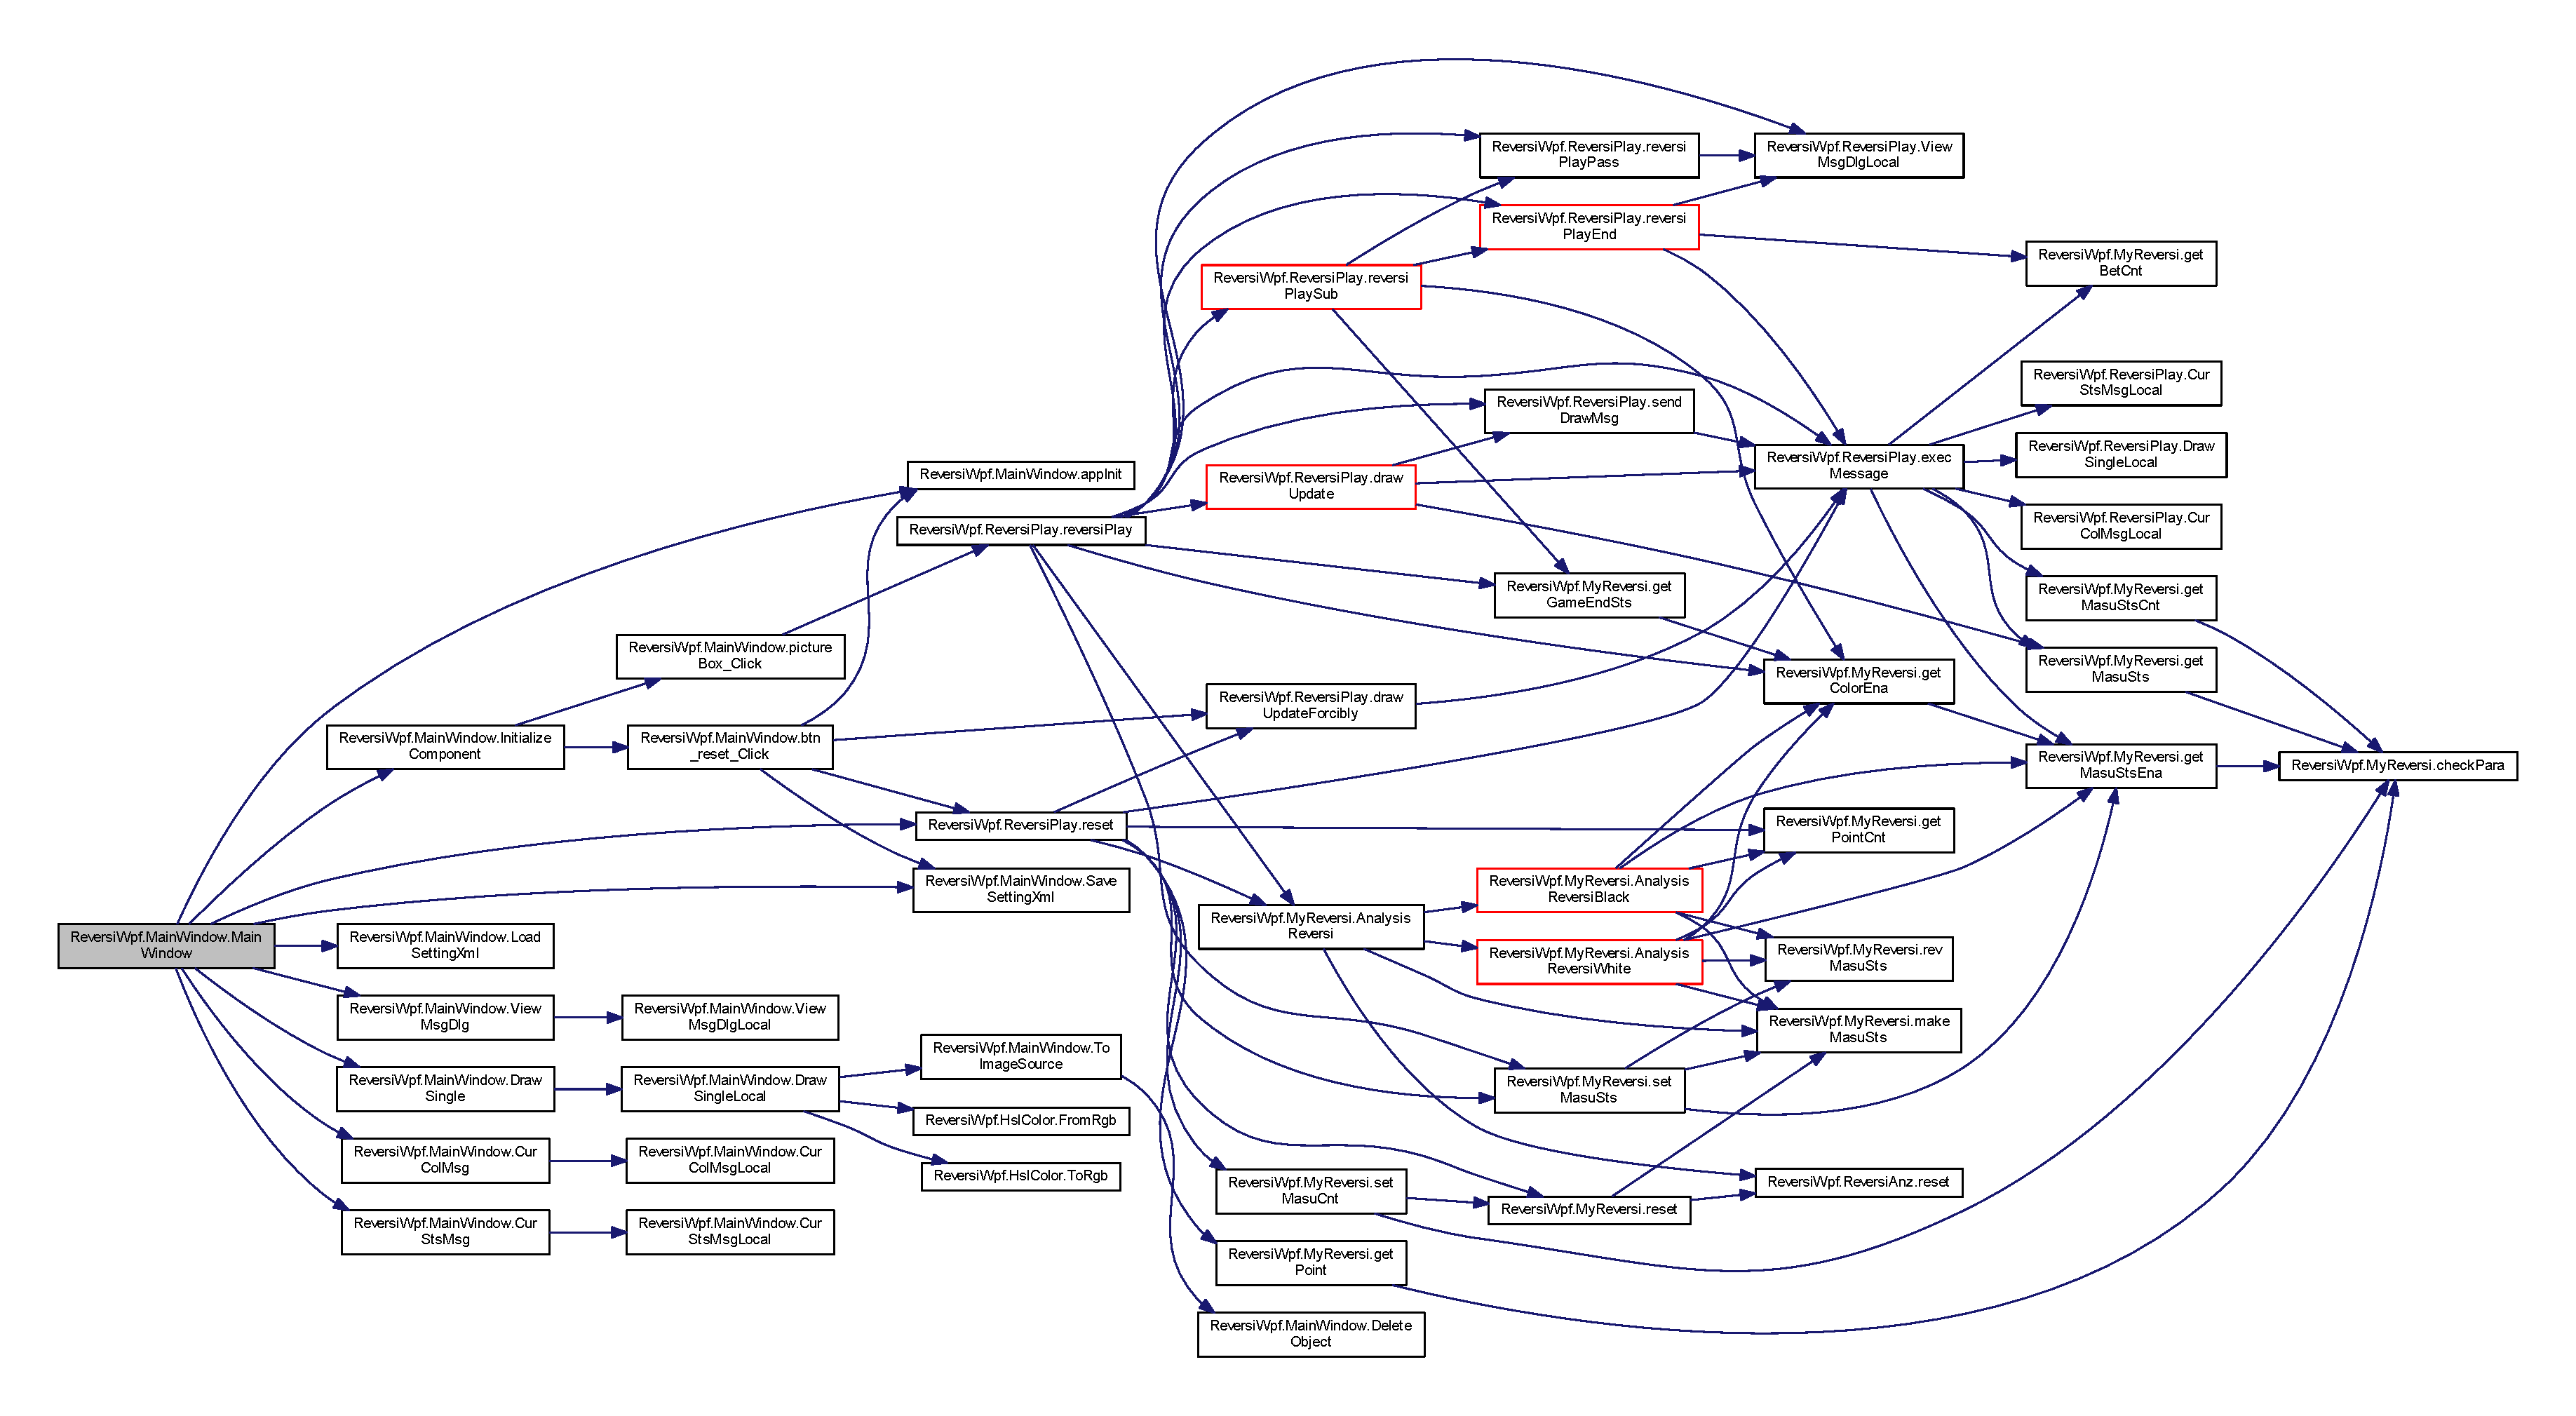
\includegraphics[width=350pt]{class_reversi_wpf_1_1_main_window_af64ecb3857a3d547b4020e9900048360_cgraph}
\end{center}
\end{figure}


\subsection{Member Function Documentation}
\mbox{\Hypertarget{class_reversi_wpf_1_1_main_window_a4e9c1014738c9b72f093dbc179ce984e}\label{class_reversi_wpf_1_1_main_window_a4e9c1014738c9b72f093dbc179ce984e}} 
\index{Reversi\+Wpf\+::\+Main\+Window@{Reversi\+Wpf\+::\+Main\+Window}!app\+Init@{app\+Init}}
\index{app\+Init@{app\+Init}!Reversi\+Wpf\+::\+Main\+Window@{Reversi\+Wpf\+::\+Main\+Window}}
\subsubsection{\texorpdfstring{app\+Init()}{appInit()}}
{\footnotesize\ttfamily void Reversi\+Wpf.\+Main\+Window.\+app\+Init (\begin{DoxyParamCaption}{ }\end{DoxyParamCaption})}



アプリ初期化 

\begin{DoxyReturn}{Returns}
ありません 
\end{DoxyReturn}
\begin{DoxyAuthor}{Author}
Yuta Yoshinaga 
\end{DoxyAuthor}
\begin{DoxyDate}{Date}
2017.\+10.\+20 
\end{DoxyDate}


Definition at line 197 of file Main\+Window.\+xaml.\+cs.



Referenced by Reversi\+Wpf.\+Main\+Window.\+btn\+\_\+reset\+\_\+\+Click(), and Reversi\+Wpf.\+Main\+Window.\+Main\+Window().

Here is the caller graph for this function\+:
\nopagebreak
\begin{figure}[H]
\begin{center}
\leavevmode
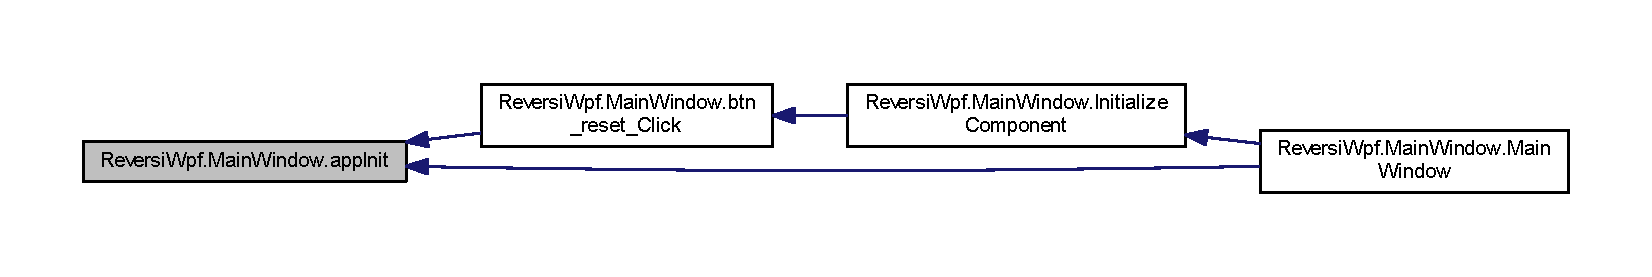
\includegraphics[width=350pt]{class_reversi_wpf_1_1_main_window_a4e9c1014738c9b72f093dbc179ce984e_icgraph}
\end{center}
\end{figure}
\mbox{\Hypertarget{class_reversi_wpf_1_1_main_window_a9b7c6af889d570bc68dcd2cf981e4cf8}\label{class_reversi_wpf_1_1_main_window_a9b7c6af889d570bc68dcd2cf981e4cf8}} 
\index{Reversi\+Wpf\+::\+Main\+Window@{Reversi\+Wpf\+::\+Main\+Window}!btn\+\_\+reset\+\_\+\+Click@{btn\+\_\+reset\+\_\+\+Click}}
\index{btn\+\_\+reset\+\_\+\+Click@{btn\+\_\+reset\+\_\+\+Click}!Reversi\+Wpf\+::\+Main\+Window@{Reversi\+Wpf\+::\+Main\+Window}}
\subsubsection{\texorpdfstring{btn\+\_\+reset\+\_\+\+Click()}{btn\_reset\_Click()}}
{\footnotesize\ttfamily void Reversi\+Wpf.\+Main\+Window.\+btn\+\_\+reset\+\_\+\+Click (\begin{DoxyParamCaption}\item[{object}]{sender,  }\item[{Routed\+Event\+Args}]{e }\end{DoxyParamCaption})\hspace{0.3cm}{\ttfamily [private]}}



リセットクリック 


\begin{DoxyParams}[1]{Parameters}
\mbox{\tt in}  & {\em object} & sender \\
\hline
\mbox{\tt in}  & {\em Routed\+Event\+Args} & e \\
\hline
\end{DoxyParams}
\begin{DoxyReturn}{Returns}
ありません 
\end{DoxyReturn}
\begin{DoxyAuthor}{Author}
Yuta Yoshinaga 
\end{DoxyAuthor}
\begin{DoxyDate}{Date}
2017.\+10.\+20 
\end{DoxyDate}


Definition at line 517 of file Main\+Window.\+xaml.\+cs.



Referenced by Reversi\+Wpf.\+Main\+Window.\+Initialize\+Component().

Here is the call graph for this function\+:
\nopagebreak
\begin{figure}[H]
\begin{center}
\leavevmode
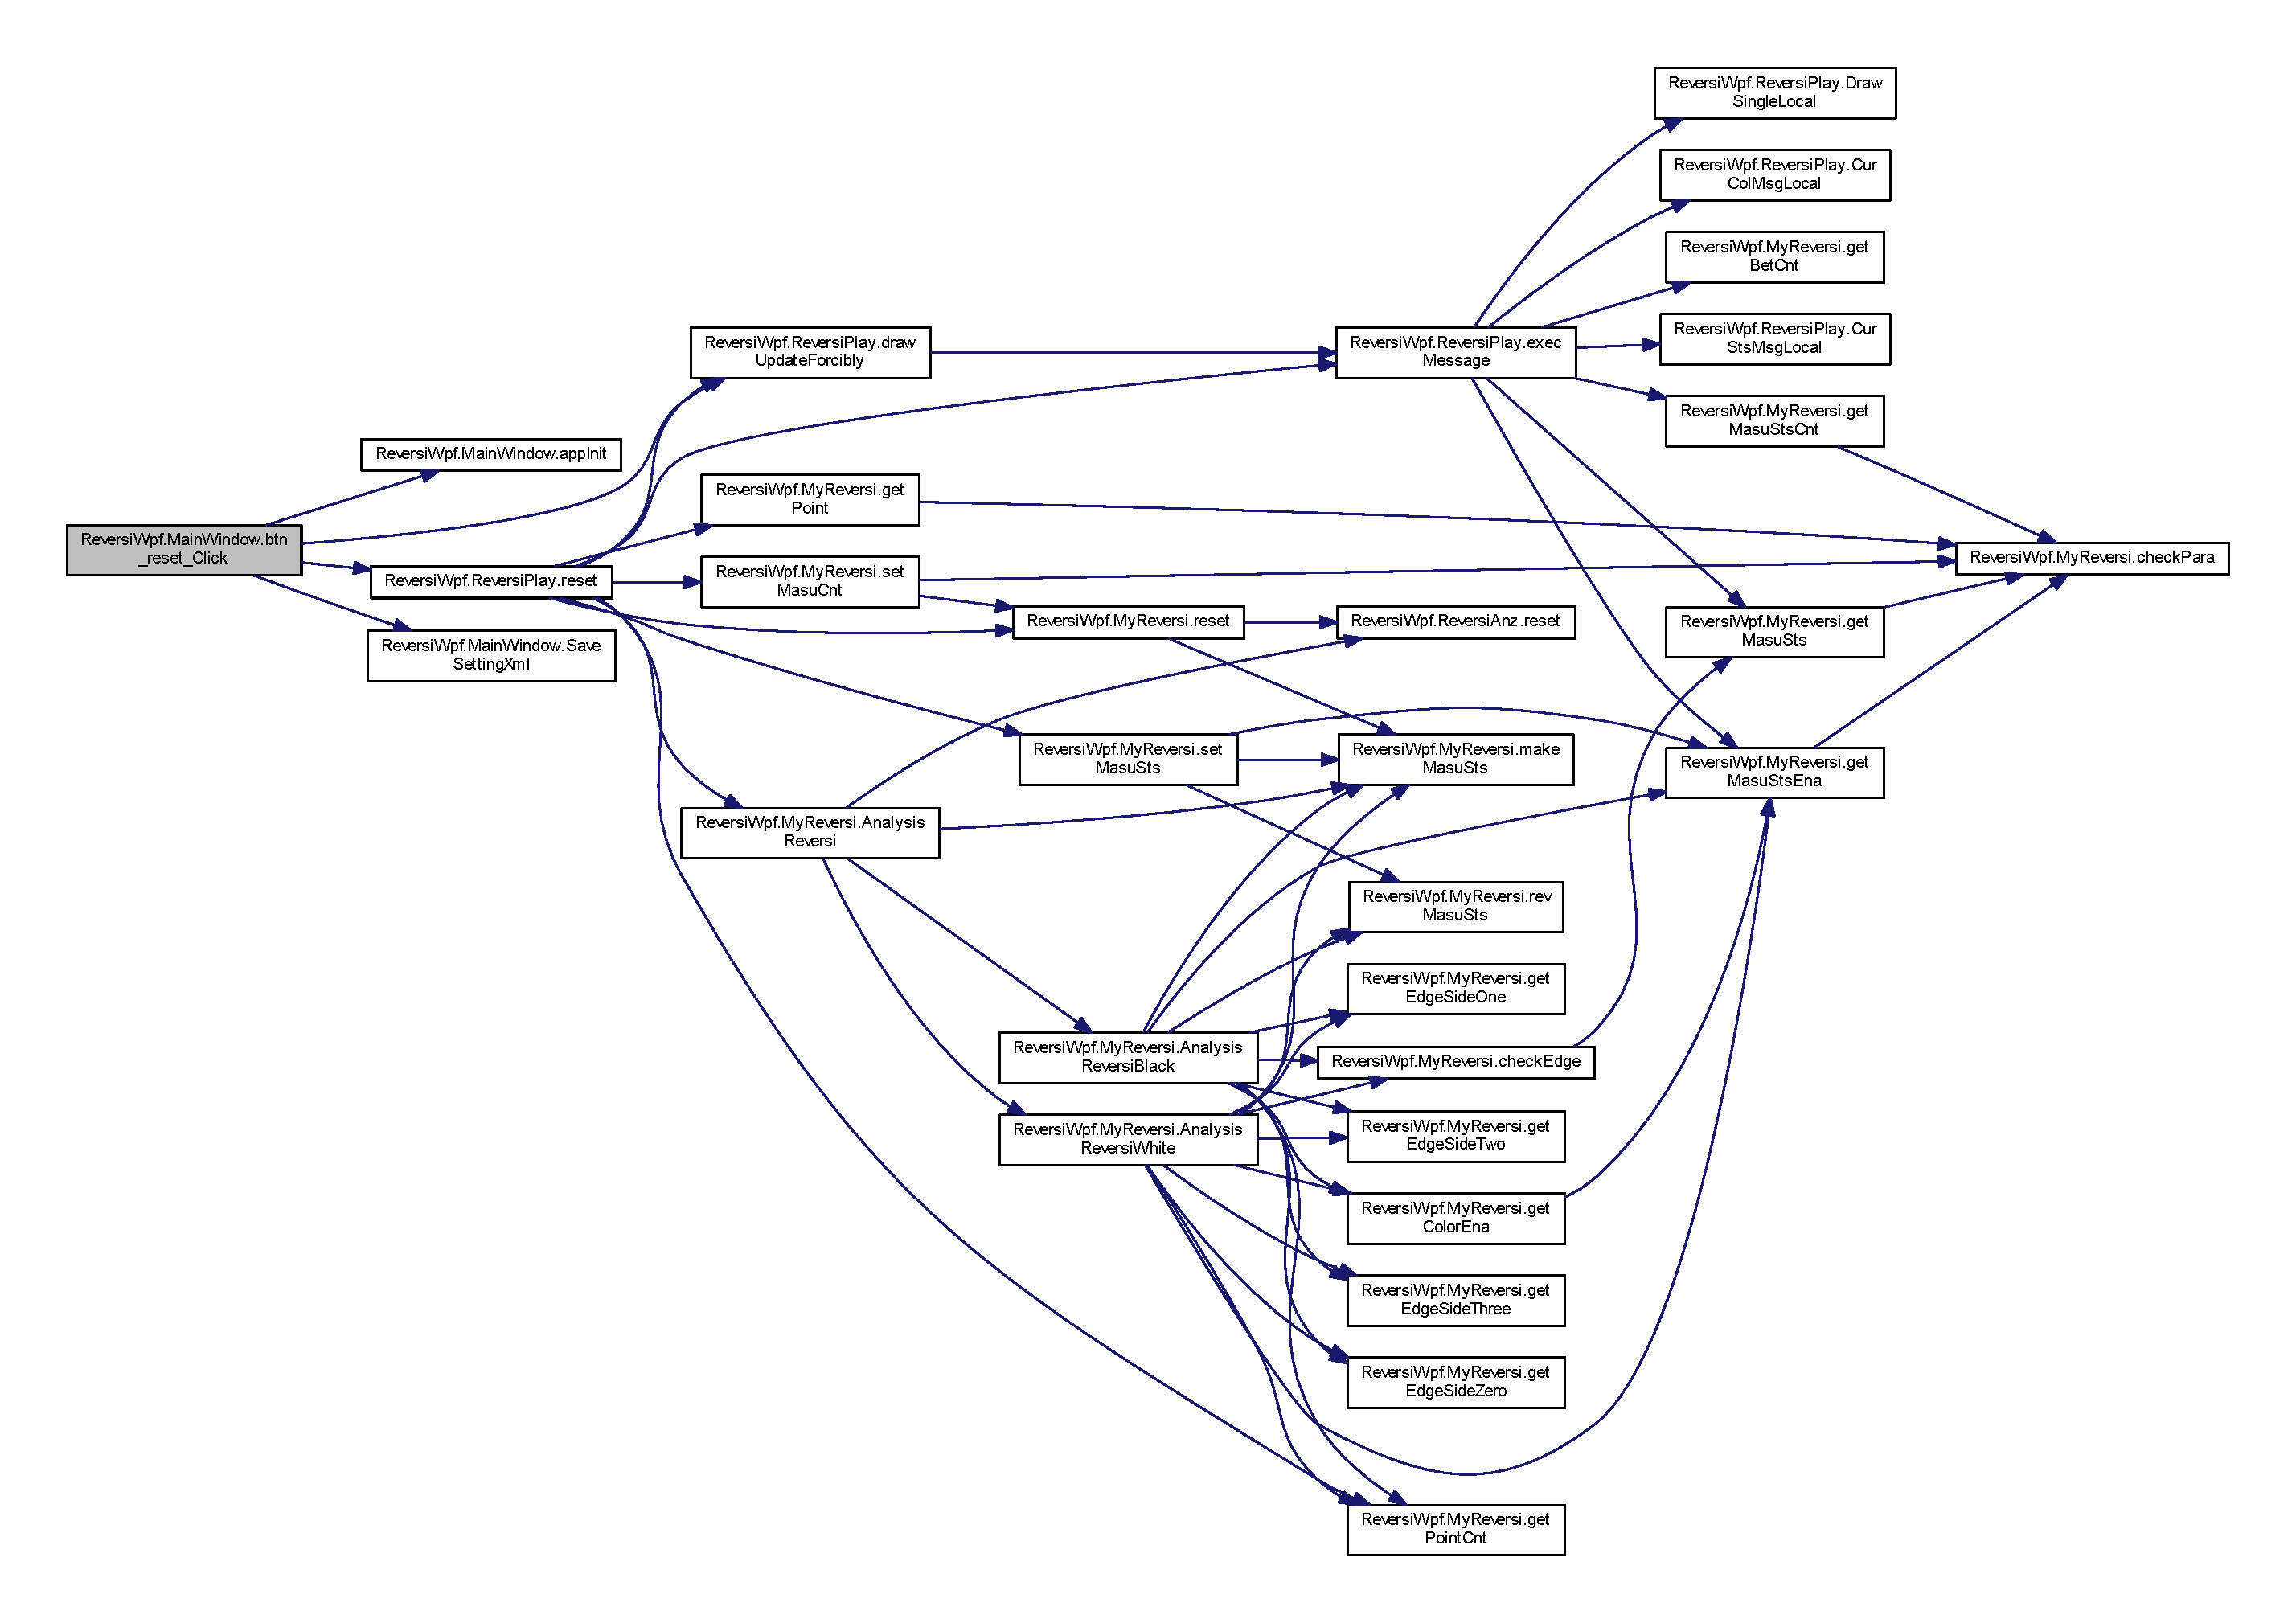
\includegraphics[width=350pt]{class_reversi_wpf_1_1_main_window_a9b7c6af889d570bc68dcd2cf981e4cf8_cgraph}
\end{center}
\end{figure}
Here is the caller graph for this function\+:
\nopagebreak
\begin{figure}[H]
\begin{center}
\leavevmode
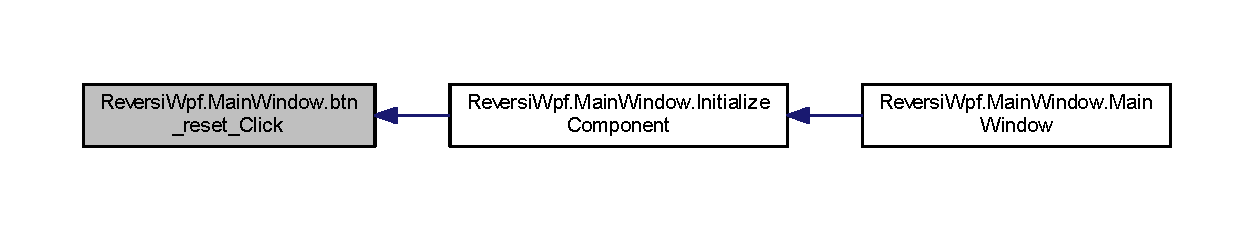
\includegraphics[width=350pt]{class_reversi_wpf_1_1_main_window_a9b7c6af889d570bc68dcd2cf981e4cf8_icgraph}
\end{center}
\end{figure}
\mbox{\Hypertarget{class_reversi_wpf_1_1_main_window_a5dd2bbfd5f17c36d1b301fdb91b483ad}\label{class_reversi_wpf_1_1_main_window_a5dd2bbfd5f17c36d1b301fdb91b483ad}} 
\index{Reversi\+Wpf\+::\+Main\+Window@{Reversi\+Wpf\+::\+Main\+Window}!Cur\+Col\+Msg@{Cur\+Col\+Msg}}
\index{Cur\+Col\+Msg@{Cur\+Col\+Msg}!Reversi\+Wpf\+::\+Main\+Window@{Reversi\+Wpf\+::\+Main\+Window}}
\subsubsection{\texorpdfstring{Cur\+Col\+Msg()}{CurColMsg()}}
{\footnotesize\ttfamily void Reversi\+Wpf.\+Main\+Window.\+Cur\+Col\+Msg (\begin{DoxyParamCaption}\item[{string}]{text }\end{DoxyParamCaption})}



現在の色メッセージ 


\begin{DoxyParams}[1]{Parameters}
\mbox{\tt in}  & {\em string} & text テキスト \\
\hline
\end{DoxyParams}
\begin{DoxyReturn}{Returns}
ありません 
\end{DoxyReturn}
\begin{DoxyAuthor}{Author}
Yuta Yoshinaga 
\end{DoxyAuthor}
\begin{DoxyDate}{Date}
2017.\+10.\+20 
\end{DoxyDate}


Definition at line 437 of file Main\+Window.\+xaml.\+cs.



Referenced by Reversi\+Wpf.\+Main\+Window.\+Main\+Window().

Here is the call graph for this function\+:
\nopagebreak
\begin{figure}[H]
\begin{center}
\leavevmode
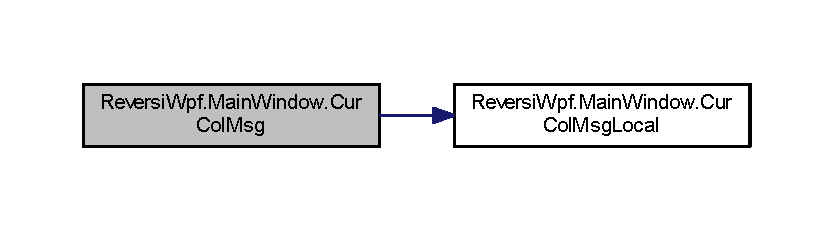
\includegraphics[width=350pt]{class_reversi_wpf_1_1_main_window_a5dd2bbfd5f17c36d1b301fdb91b483ad_cgraph}
\end{center}
\end{figure}
Here is the caller graph for this function\+:
\nopagebreak
\begin{figure}[H]
\begin{center}
\leavevmode
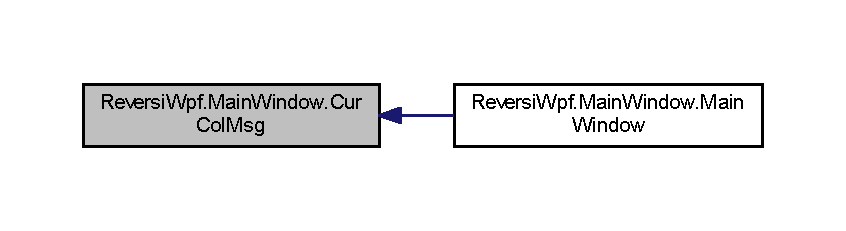
\includegraphics[width=350pt]{class_reversi_wpf_1_1_main_window_a5dd2bbfd5f17c36d1b301fdb91b483ad_icgraph}
\end{center}
\end{figure}
\mbox{\Hypertarget{class_reversi_wpf_1_1_main_window_a92d45fe8b0224e36ce974e04388ec541}\label{class_reversi_wpf_1_1_main_window_a92d45fe8b0224e36ce974e04388ec541}} 
\index{Reversi\+Wpf\+::\+Main\+Window@{Reversi\+Wpf\+::\+Main\+Window}!Cur\+Col\+Msg\+Local@{Cur\+Col\+Msg\+Local}}
\index{Cur\+Col\+Msg\+Local@{Cur\+Col\+Msg\+Local}!Reversi\+Wpf\+::\+Main\+Window@{Reversi\+Wpf\+::\+Main\+Window}}
\subsubsection{\texorpdfstring{Cur\+Col\+Msg\+Local()}{CurColMsgLocal()}}
{\footnotesize\ttfamily void Reversi\+Wpf.\+Main\+Window.\+Cur\+Col\+Msg\+Local (\begin{DoxyParamCaption}\item[{string}]{text }\end{DoxyParamCaption})}



現在の色メッセージ 


\begin{DoxyParams}[1]{Parameters}
\mbox{\tt in}  & {\em string} & text テキスト \\
\hline
\end{DoxyParams}
\begin{DoxyReturn}{Returns}
ありません 
\end{DoxyReturn}
\begin{DoxyAuthor}{Author}
Yuta Yoshinaga 
\end{DoxyAuthor}
\begin{DoxyDate}{Date}
2017.\+10.\+20 
\end{DoxyDate}


Definition at line 451 of file Main\+Window.\+xaml.\+cs.



Referenced by Reversi\+Wpf.\+Main\+Window.\+Cur\+Col\+Msg().

Here is the caller graph for this function\+:
\nopagebreak
\begin{figure}[H]
\begin{center}
\leavevmode
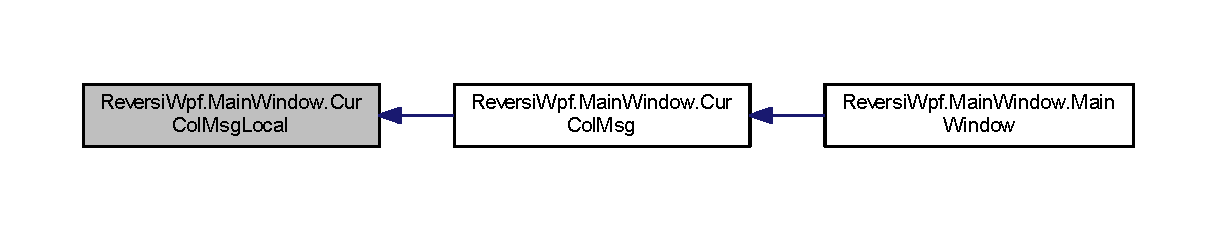
\includegraphics[width=350pt]{class_reversi_wpf_1_1_main_window_a92d45fe8b0224e36ce974e04388ec541_icgraph}
\end{center}
\end{figure}
\mbox{\Hypertarget{class_reversi_wpf_1_1_main_window_a90e6aa75849526159fe9348da2b66fb0}\label{class_reversi_wpf_1_1_main_window_a90e6aa75849526159fe9348da2b66fb0}} 
\index{Reversi\+Wpf\+::\+Main\+Window@{Reversi\+Wpf\+::\+Main\+Window}!Cur\+Sts\+Msg@{Cur\+Sts\+Msg}}
\index{Cur\+Sts\+Msg@{Cur\+Sts\+Msg}!Reversi\+Wpf\+::\+Main\+Window@{Reversi\+Wpf\+::\+Main\+Window}}
\subsubsection{\texorpdfstring{Cur\+Sts\+Msg()}{CurStsMsg()}}
{\footnotesize\ttfamily void Reversi\+Wpf.\+Main\+Window.\+Cur\+Sts\+Msg (\begin{DoxyParamCaption}\item[{string}]{text }\end{DoxyParamCaption})}



現在のステータスメッセージ 


\begin{DoxyParams}[1]{Parameters}
\mbox{\tt in}  & {\em string} & text テキスト \\
\hline
\end{DoxyParams}
\begin{DoxyReturn}{Returns}
ありません 
\end{DoxyReturn}
\begin{DoxyAuthor}{Author}
Yuta Yoshinaga 
\end{DoxyAuthor}
\begin{DoxyDate}{Date}
2017.\+10.\+20 
\end{DoxyDate}


Definition at line 465 of file Main\+Window.\+xaml.\+cs.



Referenced by Reversi\+Wpf.\+Main\+Window.\+Main\+Window().

Here is the call graph for this function\+:
\nopagebreak
\begin{figure}[H]
\begin{center}
\leavevmode
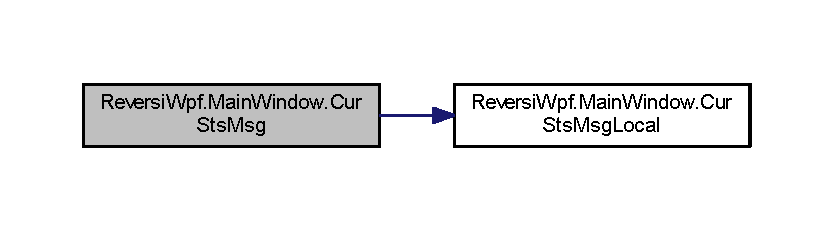
\includegraphics[width=350pt]{class_reversi_wpf_1_1_main_window_a90e6aa75849526159fe9348da2b66fb0_cgraph}
\end{center}
\end{figure}
Here is the caller graph for this function\+:
\nopagebreak
\begin{figure}[H]
\begin{center}
\leavevmode
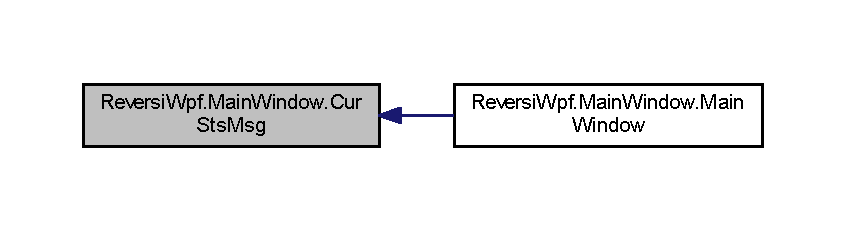
\includegraphics[width=350pt]{class_reversi_wpf_1_1_main_window_a90e6aa75849526159fe9348da2b66fb0_icgraph}
\end{center}
\end{figure}
\mbox{\Hypertarget{class_reversi_wpf_1_1_main_window_a73402ffecf2de584339327dce357bd60}\label{class_reversi_wpf_1_1_main_window_a73402ffecf2de584339327dce357bd60}} 
\index{Reversi\+Wpf\+::\+Main\+Window@{Reversi\+Wpf\+::\+Main\+Window}!Cur\+Sts\+Msg\+Local@{Cur\+Sts\+Msg\+Local}}
\index{Cur\+Sts\+Msg\+Local@{Cur\+Sts\+Msg\+Local}!Reversi\+Wpf\+::\+Main\+Window@{Reversi\+Wpf\+::\+Main\+Window}}
\subsubsection{\texorpdfstring{Cur\+Sts\+Msg\+Local()}{CurStsMsgLocal()}}
{\footnotesize\ttfamily void Reversi\+Wpf.\+Main\+Window.\+Cur\+Sts\+Msg\+Local (\begin{DoxyParamCaption}\item[{string}]{text }\end{DoxyParamCaption})}



現在のステータスメッセージ 


\begin{DoxyParams}[1]{Parameters}
\mbox{\tt in}  & {\em string} & text テキスト \\
\hline
\end{DoxyParams}
\begin{DoxyReturn}{Returns}
ありません 
\end{DoxyReturn}
\begin{DoxyAuthor}{Author}
Yuta Yoshinaga 
\end{DoxyAuthor}
\begin{DoxyDate}{Date}
2017.\+10.\+20 
\end{DoxyDate}


Definition at line 479 of file Main\+Window.\+xaml.\+cs.



Referenced by Reversi\+Wpf.\+Main\+Window.\+Cur\+Sts\+Msg().

Here is the caller graph for this function\+:
\nopagebreak
\begin{figure}[H]
\begin{center}
\leavevmode
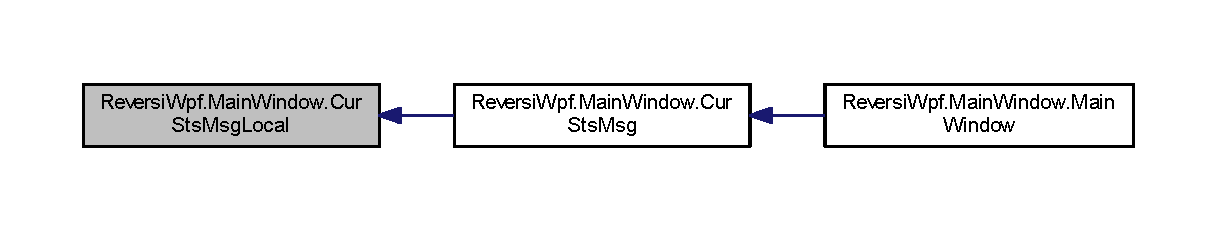
\includegraphics[width=350pt]{class_reversi_wpf_1_1_main_window_a73402ffecf2de584339327dce357bd60_icgraph}
\end{center}
\end{figure}
\mbox{\Hypertarget{class_reversi_wpf_1_1_main_window_aa7f29f9037ca59f0b41d4b383875bb5e}\label{class_reversi_wpf_1_1_main_window_aa7f29f9037ca59f0b41d4b383875bb5e}} 
\index{Reversi\+Wpf\+::\+Main\+Window@{Reversi\+Wpf\+::\+Main\+Window}!Draw\+Single@{Draw\+Single}}
\index{Draw\+Single@{Draw\+Single}!Reversi\+Wpf\+::\+Main\+Window@{Reversi\+Wpf\+::\+Main\+Window}}
\subsubsection{\texorpdfstring{Draw\+Single()}{DrawSingle()}}
{\footnotesize\ttfamily void Reversi\+Wpf.\+Main\+Window.\+Draw\+Single (\begin{DoxyParamCaption}\item[{int}]{y,  }\item[{int}]{x,  }\item[{int}]{sts,  }\item[{int}]{bk,  }\item[{string}]{text }\end{DoxyParamCaption})}



1マス描画 


\begin{DoxyParams}[1]{Parameters}
\mbox{\tt in}  & {\em int} & y Y座標 \\
\hline
\mbox{\tt in}  & {\em int} & x X座標 \\
\hline
\mbox{\tt in}  & {\em int} & sts ステータス \\
\hline
\mbox{\tt in}  & {\em int} & bk 背景 \\
\hline
\mbox{\tt in}  & {\em string} & text テキスト \\
\hline
\end{DoxyParams}
\begin{DoxyReturn}{Returns}
ありません 
\end{DoxyReturn}
\begin{DoxyAuthor}{Author}
Yuta Yoshinaga 
\end{DoxyAuthor}
\begin{DoxyDate}{Date}
2017.\+10.\+20 
\end{DoxyDate}


Definition at line 298 of file Main\+Window.\+xaml.\+cs.



Referenced by Reversi\+Wpf.\+Main\+Window.\+Main\+Window().

Here is the call graph for this function\+:
\nopagebreak
\begin{figure}[H]
\begin{center}
\leavevmode
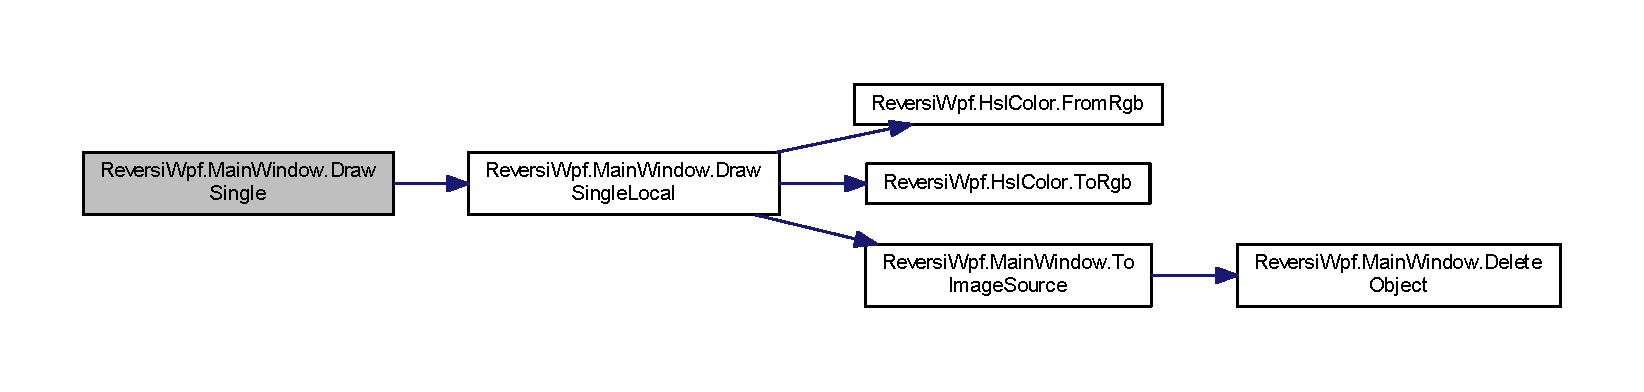
\includegraphics[width=350pt]{class_reversi_wpf_1_1_main_window_aa7f29f9037ca59f0b41d4b383875bb5e_cgraph}
\end{center}
\end{figure}
Here is the caller graph for this function\+:
\nopagebreak
\begin{figure}[H]
\begin{center}
\leavevmode
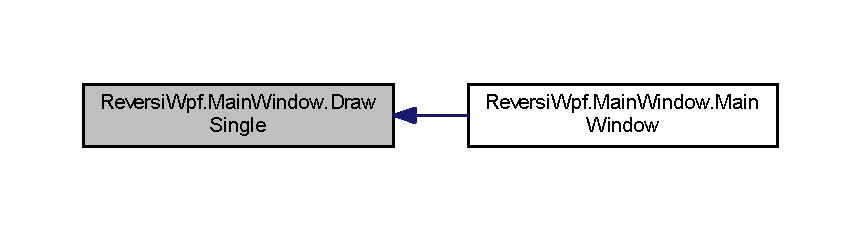
\includegraphics[width=350pt]{class_reversi_wpf_1_1_main_window_aa7f29f9037ca59f0b41d4b383875bb5e_icgraph}
\end{center}
\end{figure}
\mbox{\Hypertarget{class_reversi_wpf_1_1_main_window_a88fd4a18ce06e08801a3370147bc3a8b}\label{class_reversi_wpf_1_1_main_window_a88fd4a18ce06e08801a3370147bc3a8b}} 
\index{Reversi\+Wpf\+::\+Main\+Window@{Reversi\+Wpf\+::\+Main\+Window}!Draw\+Single\+Local@{Draw\+Single\+Local}}
\index{Draw\+Single\+Local@{Draw\+Single\+Local}!Reversi\+Wpf\+::\+Main\+Window@{Reversi\+Wpf\+::\+Main\+Window}}
\subsubsection{\texorpdfstring{Draw\+Single\+Local()}{DrawSingleLocal()}}
{\footnotesize\ttfamily void Reversi\+Wpf.\+Main\+Window.\+Draw\+Single\+Local (\begin{DoxyParamCaption}\item[{int}]{y,  }\item[{int}]{x,  }\item[{int}]{sts,  }\item[{int}]{bk,  }\item[{string}]{text }\end{DoxyParamCaption})}



1マス描画 


\begin{DoxyParams}[1]{Parameters}
\mbox{\tt in}  & {\em int} & y Y座標 \\
\hline
\mbox{\tt in}  & {\em int} & x X座標 \\
\hline
\mbox{\tt in}  & {\em int} & sts ステータス \\
\hline
\mbox{\tt in}  & {\em int} & bk 背景 \\
\hline
\mbox{\tt in}  & {\em string} & text テキスト \\
\hline
\end{DoxyParams}
\begin{DoxyReturn}{Returns}
ありません 
\end{DoxyReturn}
\begin{DoxyAuthor}{Author}
Yuta Yoshinaga 
\end{DoxyAuthor}
\begin{DoxyDate}{Date}
2017.\+10.\+20 
\end{DoxyDate}


Definition at line 316 of file Main\+Window.\+xaml.\+cs.



Referenced by Reversi\+Wpf.\+Main\+Window.\+Draw\+Single().

Here is the call graph for this function\+:
\nopagebreak
\begin{figure}[H]
\begin{center}
\leavevmode
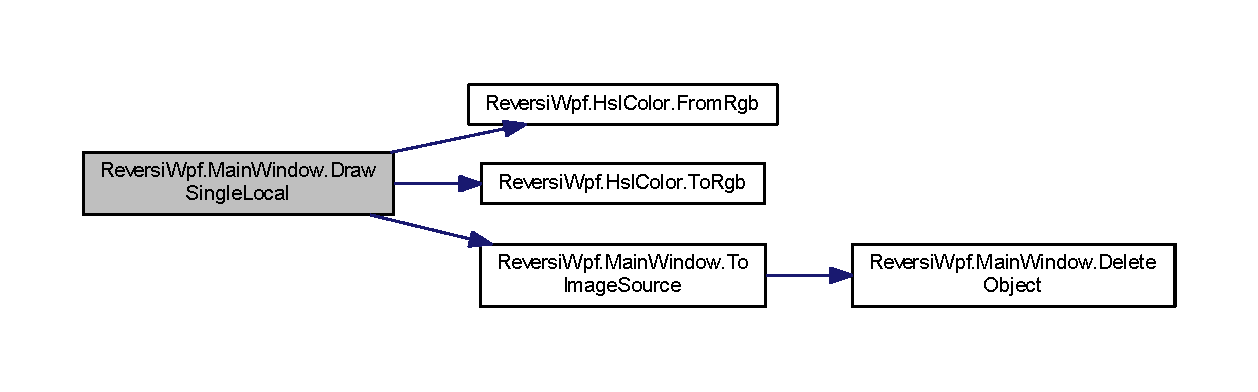
\includegraphics[width=350pt]{class_reversi_wpf_1_1_main_window_a88fd4a18ce06e08801a3370147bc3a8b_cgraph}
\end{center}
\end{figure}
Here is the caller graph for this function\+:
\nopagebreak
\begin{figure}[H]
\begin{center}
\leavevmode
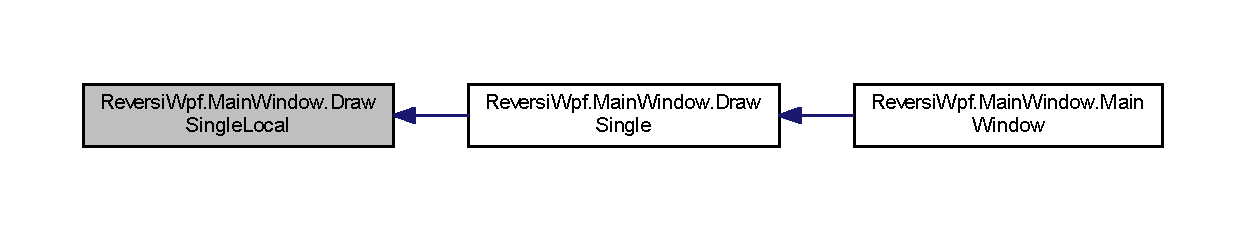
\includegraphics[width=350pt]{class_reversi_wpf_1_1_main_window_a88fd4a18ce06e08801a3370147bc3a8b_icgraph}
\end{center}
\end{figure}
\mbox{\Hypertarget{class_reversi_wpf_1_1_main_window_a4cf9bc92cee02fa8e3b00fa56fb41c82}\label{class_reversi_wpf_1_1_main_window_a4cf9bc92cee02fa8e3b00fa56fb41c82}} 
\index{Reversi\+Wpf\+::\+Main\+Window@{Reversi\+Wpf\+::\+Main\+Window}!Initialize\+Component@{Initialize\+Component}}
\index{Initialize\+Component@{Initialize\+Component}!Reversi\+Wpf\+::\+Main\+Window@{Reversi\+Wpf\+::\+Main\+Window}}
\subsubsection{\texorpdfstring{Initialize\+Component()}{InitializeComponent()}\hspace{0.1cm}{\footnotesize\ttfamily [1/4]}}
{\footnotesize\ttfamily void Reversi\+Wpf.\+Main\+Window.\+Initialize\+Component (\begin{DoxyParamCaption}{ }\end{DoxyParamCaption})}



Initialize\+Component 



Definition at line 3290 of file Main\+Window.\+g.\+cs.



Referenced by Reversi\+Wpf.\+Main\+Window.\+Main\+Window().

Here is the call graph for this function\+:
\nopagebreak
\begin{figure}[H]
\begin{center}
\leavevmode
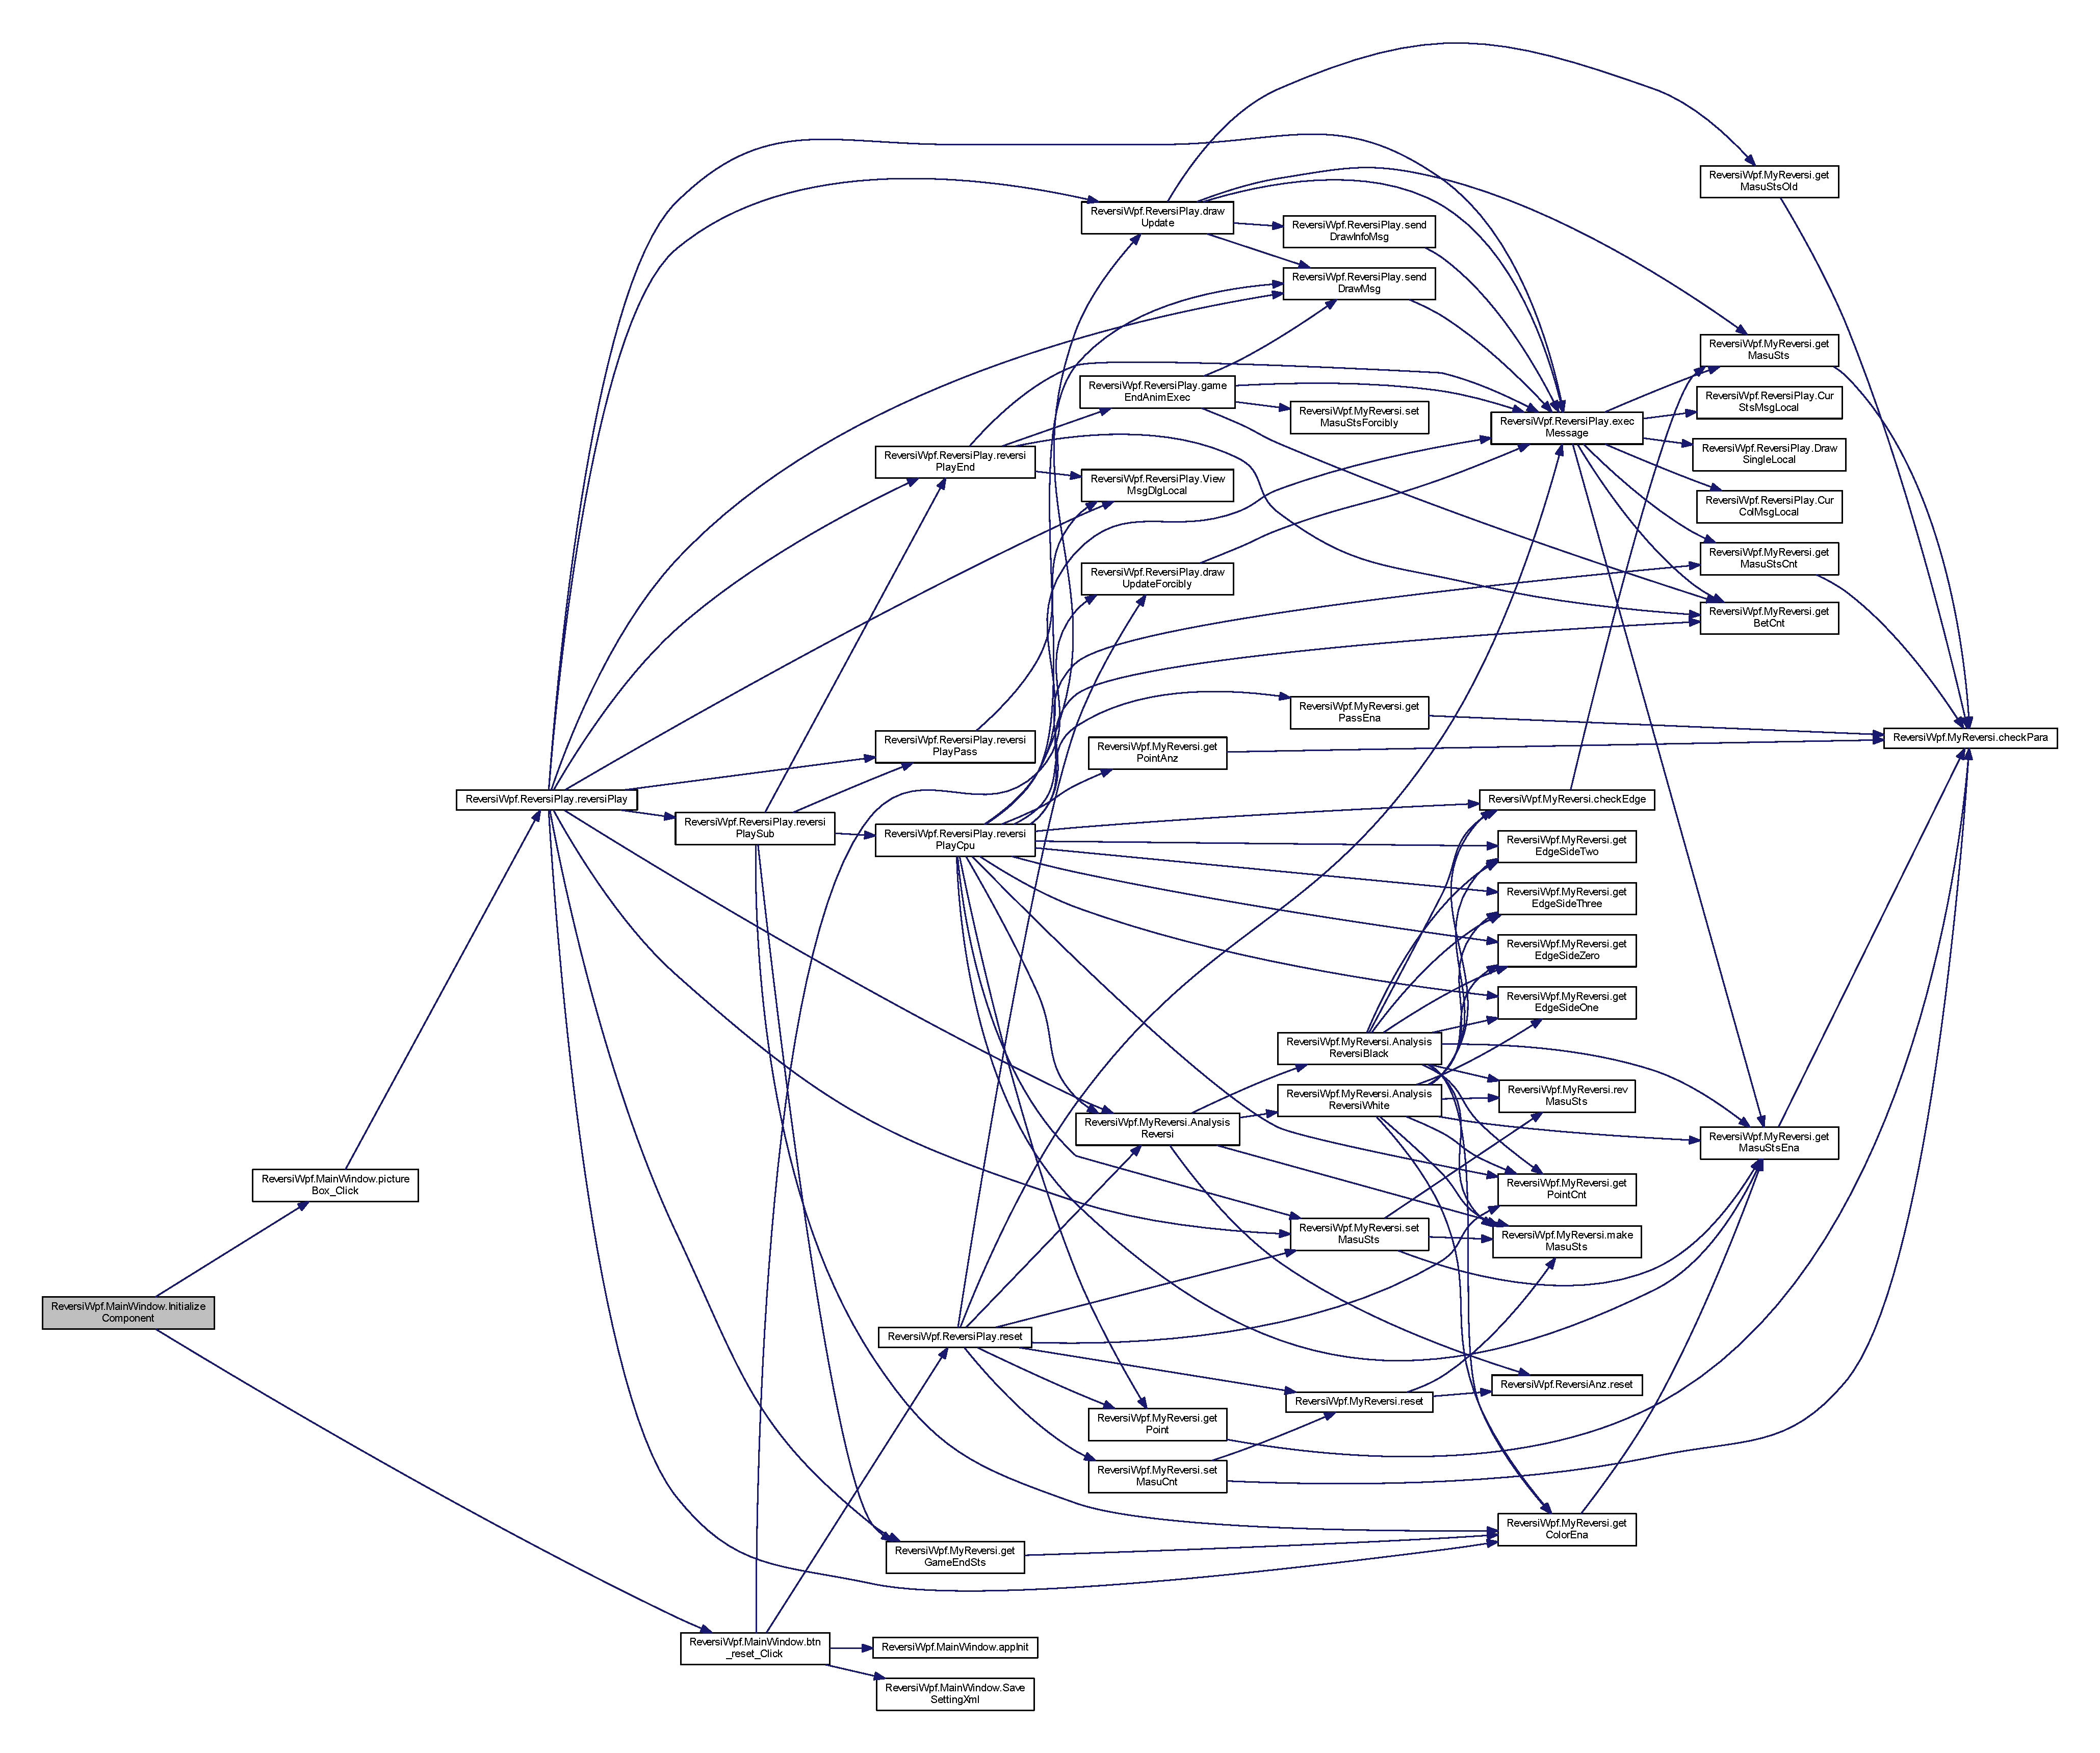
\includegraphics[width=350pt]{class_reversi_wpf_1_1_main_window_a4cf9bc92cee02fa8e3b00fa56fb41c82_cgraph}
\end{center}
\end{figure}
Here is the caller graph for this function\+:
\nopagebreak
\begin{figure}[H]
\begin{center}
\leavevmode
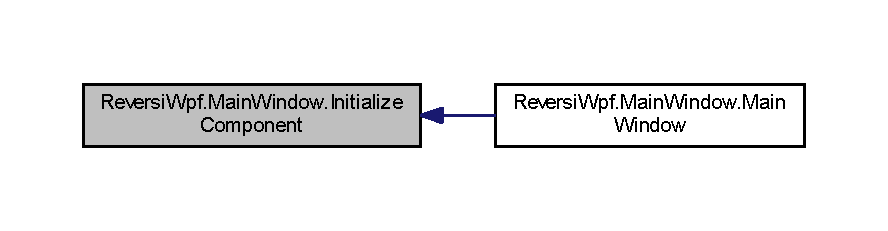
\includegraphics[width=350pt]{class_reversi_wpf_1_1_main_window_a4cf9bc92cee02fa8e3b00fa56fb41c82_icgraph}
\end{center}
\end{figure}
\mbox{\Hypertarget{class_reversi_wpf_1_1_main_window_a4cf9bc92cee02fa8e3b00fa56fb41c82}\label{class_reversi_wpf_1_1_main_window_a4cf9bc92cee02fa8e3b00fa56fb41c82}} 
\index{Reversi\+Wpf\+::\+Main\+Window@{Reversi\+Wpf\+::\+Main\+Window}!Initialize\+Component@{Initialize\+Component}}
\index{Initialize\+Component@{Initialize\+Component}!Reversi\+Wpf\+::\+Main\+Window@{Reversi\+Wpf\+::\+Main\+Window}}
\subsubsection{\texorpdfstring{Initialize\+Component()}{InitializeComponent()}\hspace{0.1cm}{\footnotesize\ttfamily [2/4]}}
{\footnotesize\ttfamily void Reversi\+Wpf.\+Main\+Window.\+Initialize\+Component (\begin{DoxyParamCaption}{ }\end{DoxyParamCaption})}



Initialize\+Component 



Definition at line 3290 of file Main\+Window.\+g.\+i.\+cs.

Here is the call graph for this function\+:
\nopagebreak
\begin{figure}[H]
\begin{center}
\leavevmode
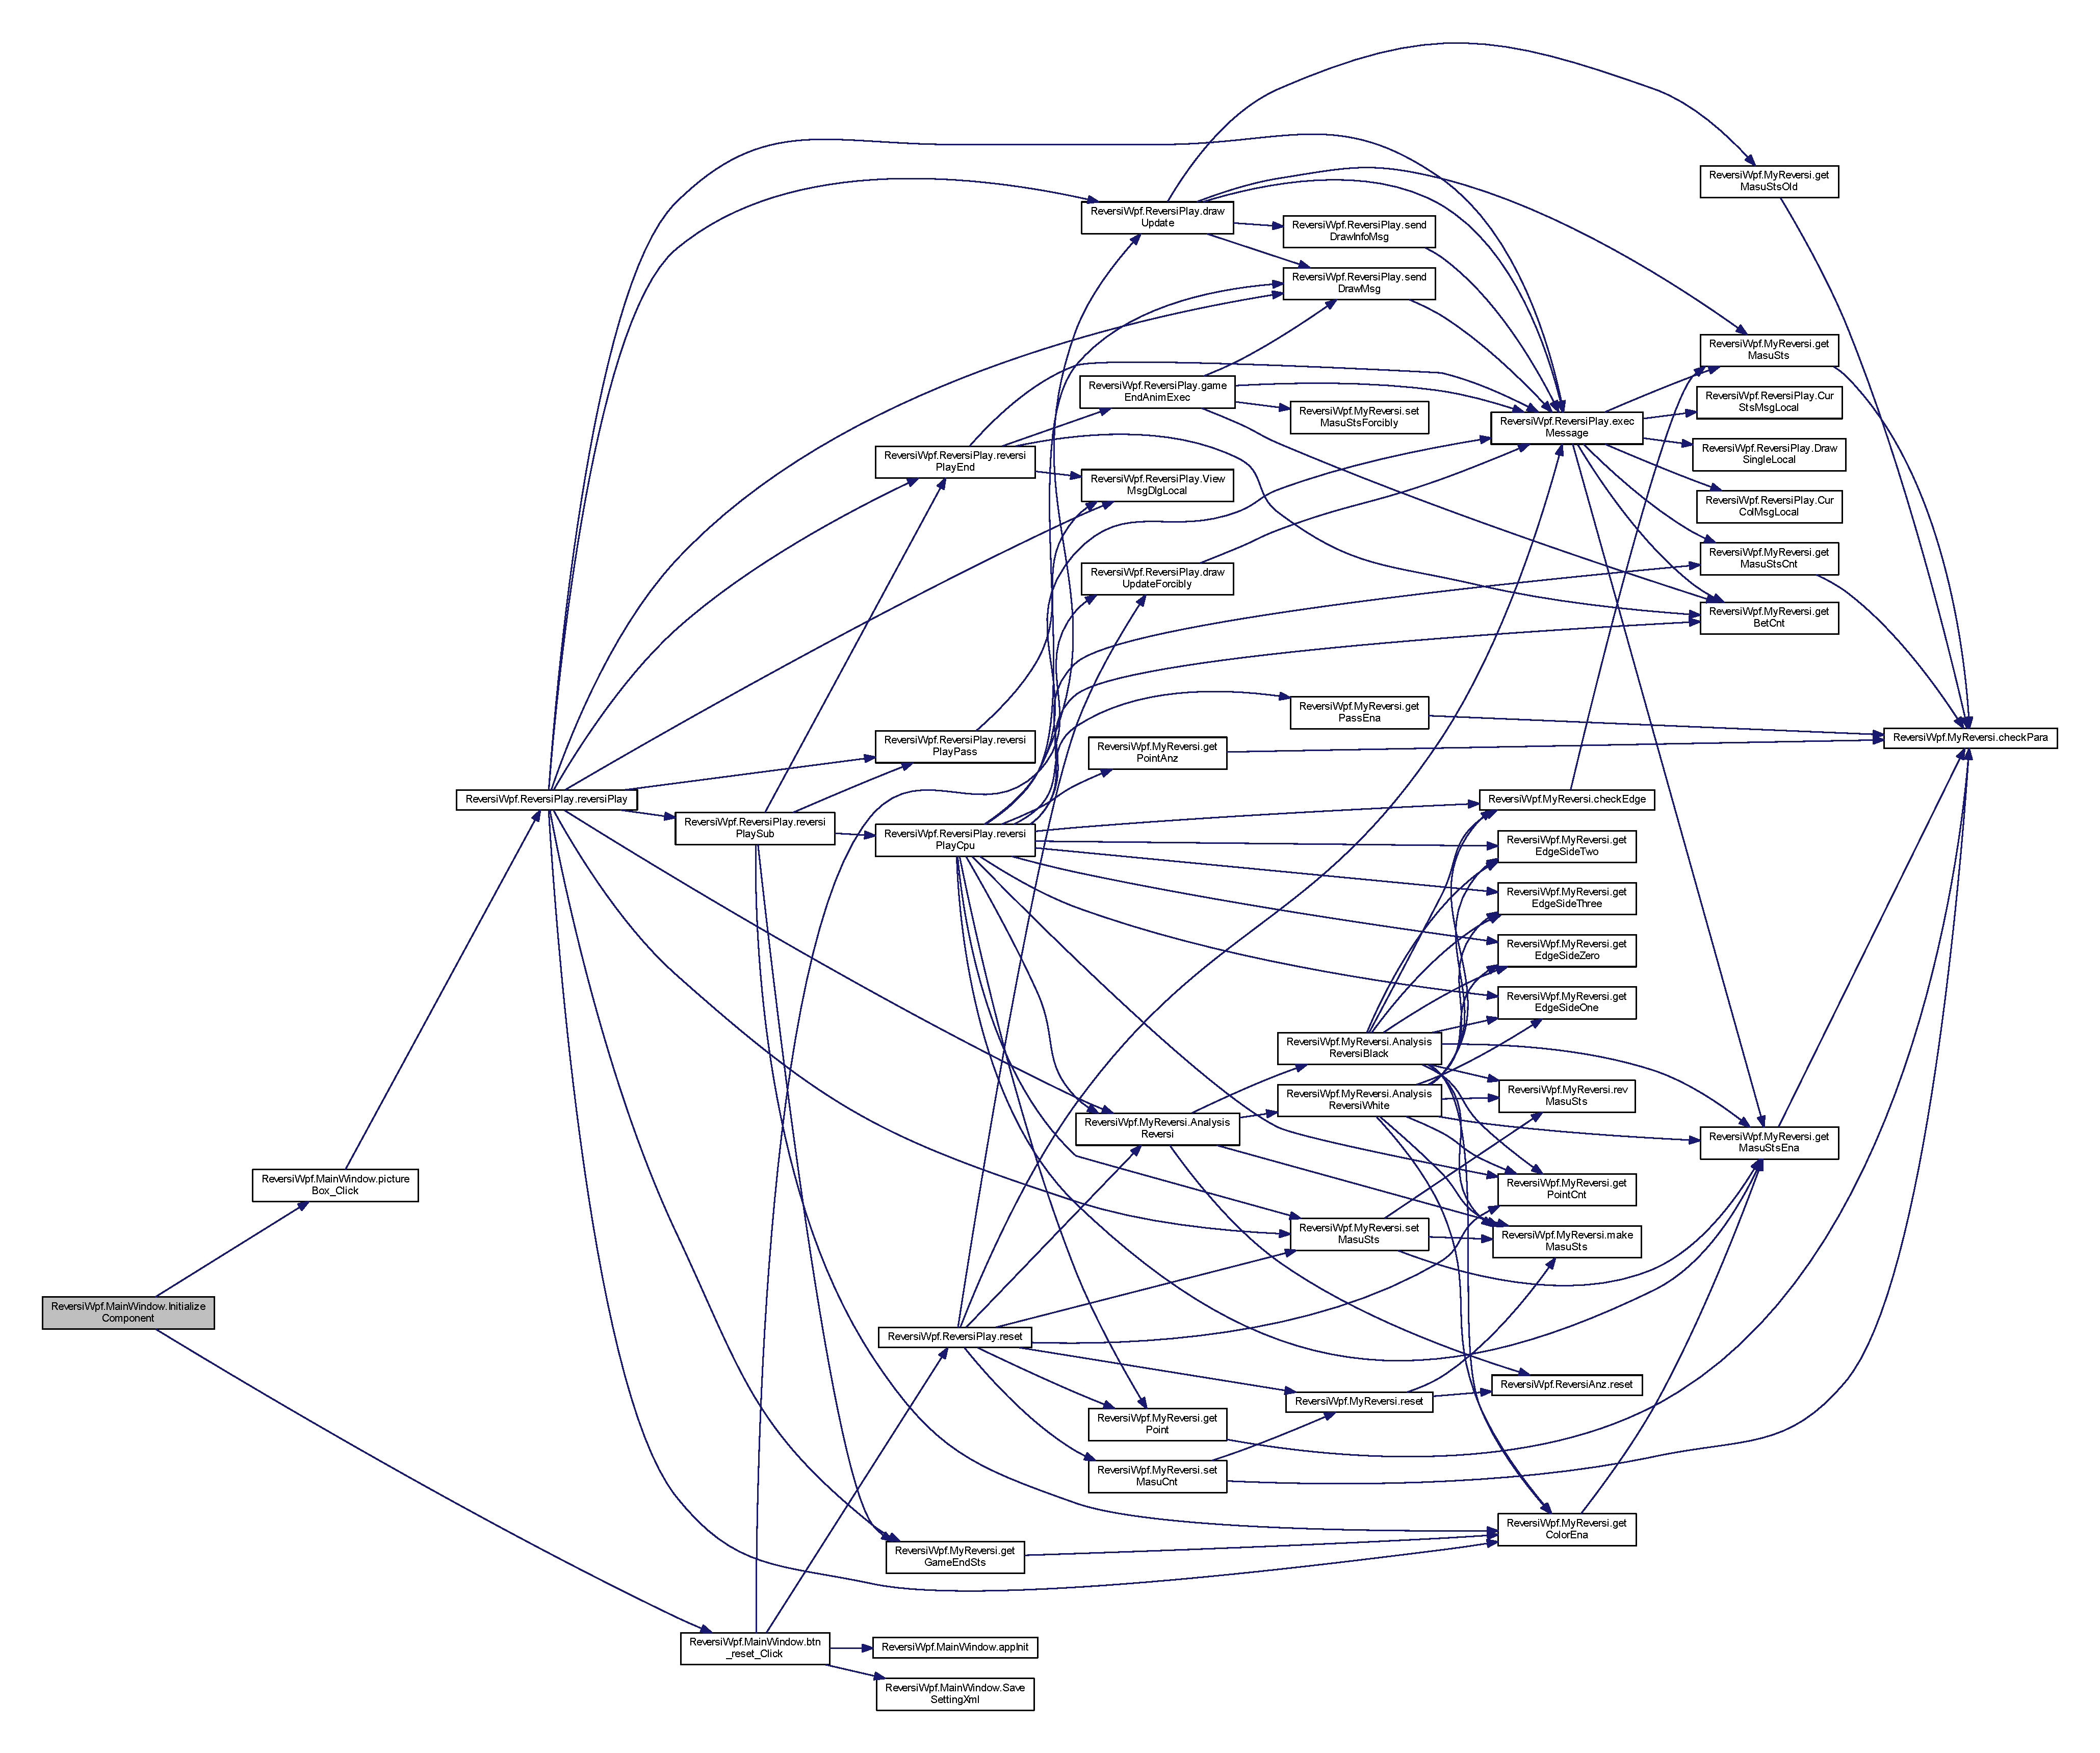
\includegraphics[width=350pt]{class_reversi_wpf_1_1_main_window_a4cf9bc92cee02fa8e3b00fa56fb41c82_cgraph}
\end{center}
\end{figure}
\mbox{\Hypertarget{class_reversi_wpf_1_1_main_window_a4cf9bc92cee02fa8e3b00fa56fb41c82}\label{class_reversi_wpf_1_1_main_window_a4cf9bc92cee02fa8e3b00fa56fb41c82}} 
\index{Reversi\+Wpf\+::\+Main\+Window@{Reversi\+Wpf\+::\+Main\+Window}!Initialize\+Component@{Initialize\+Component}}
\index{Initialize\+Component@{Initialize\+Component}!Reversi\+Wpf\+::\+Main\+Window@{Reversi\+Wpf\+::\+Main\+Window}}
\subsubsection{\texorpdfstring{Initialize\+Component()}{InitializeComponent()}\hspace{0.1cm}{\footnotesize\ttfamily [3/4]}}
{\footnotesize\ttfamily void Reversi\+Wpf.\+Main\+Window.\+Initialize\+Component (\begin{DoxyParamCaption}{ }\end{DoxyParamCaption})}



Initialize\+Component 



Definition at line 3290 of file Main\+Window.\+g.\+cs.

Here is the call graph for this function\+:
\nopagebreak
\begin{figure}[H]
\begin{center}
\leavevmode
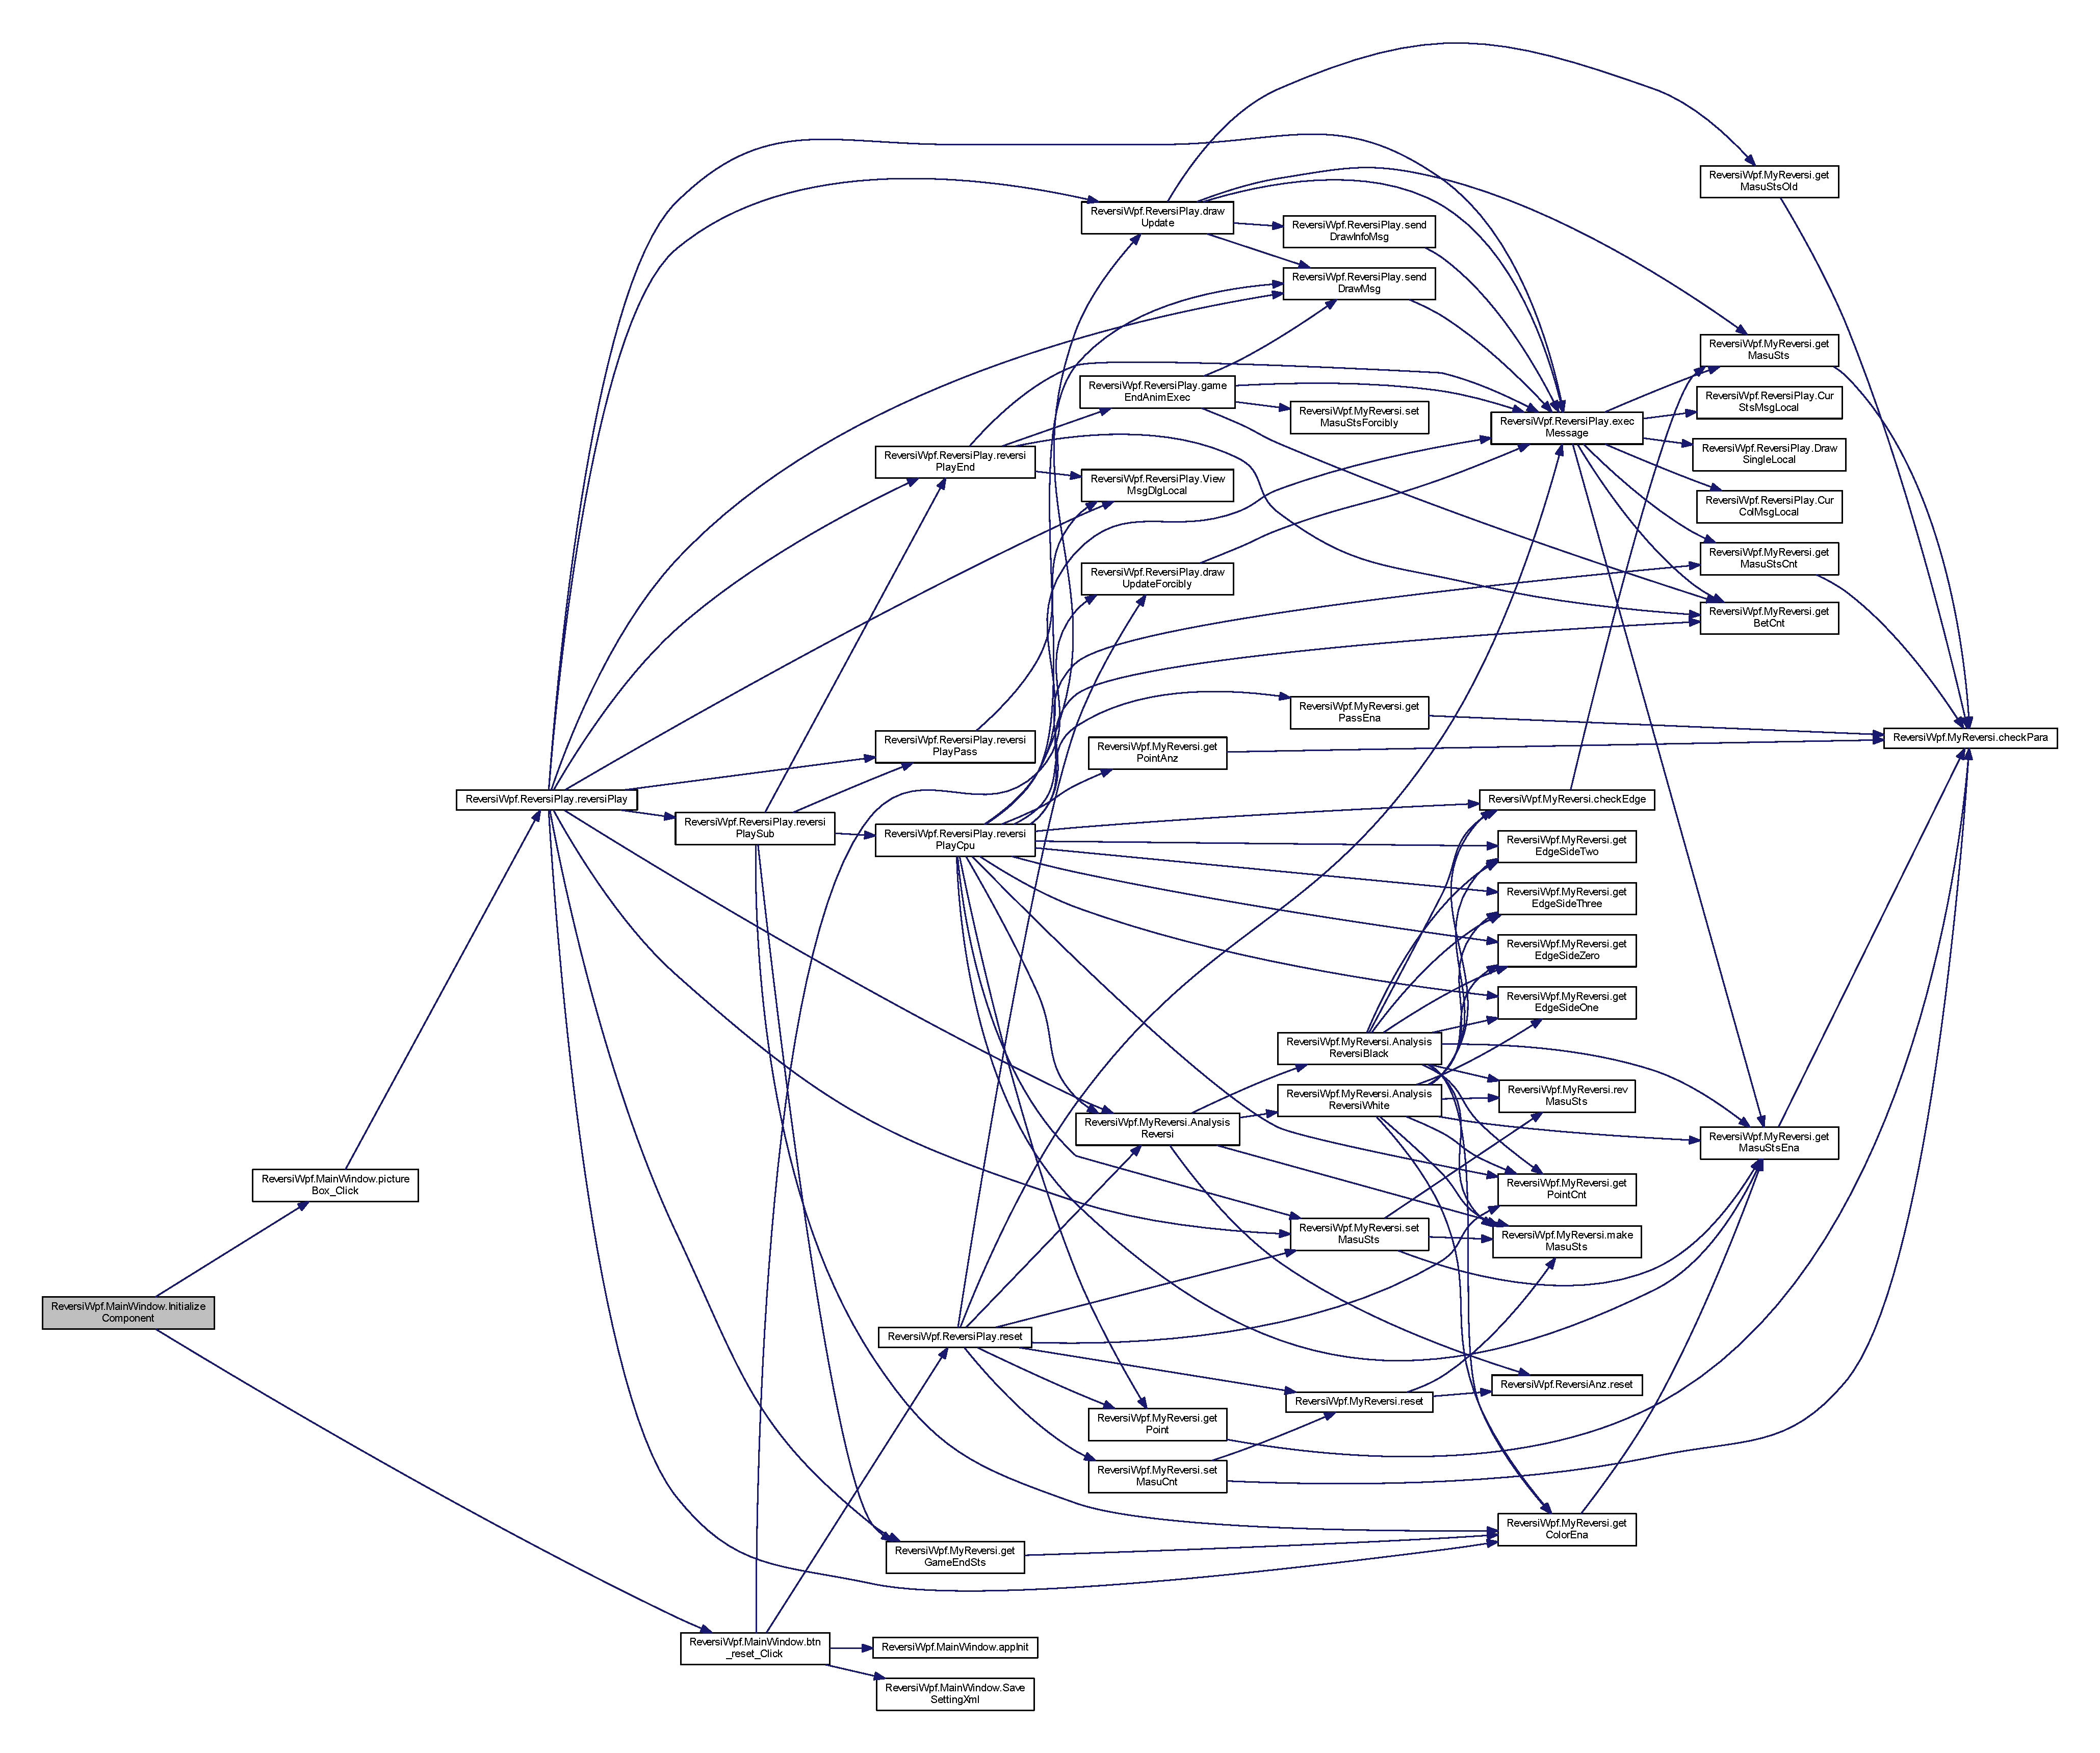
\includegraphics[width=350pt]{class_reversi_wpf_1_1_main_window_a4cf9bc92cee02fa8e3b00fa56fb41c82_cgraph}
\end{center}
\end{figure}
\mbox{\Hypertarget{class_reversi_wpf_1_1_main_window_a4cf9bc92cee02fa8e3b00fa56fb41c82}\label{class_reversi_wpf_1_1_main_window_a4cf9bc92cee02fa8e3b00fa56fb41c82}} 
\index{Reversi\+Wpf\+::\+Main\+Window@{Reversi\+Wpf\+::\+Main\+Window}!Initialize\+Component@{Initialize\+Component}}
\index{Initialize\+Component@{Initialize\+Component}!Reversi\+Wpf\+::\+Main\+Window@{Reversi\+Wpf\+::\+Main\+Window}}
\subsubsection{\texorpdfstring{Initialize\+Component()}{InitializeComponent()}\hspace{0.1cm}{\footnotesize\ttfamily [4/4]}}
{\footnotesize\ttfamily void Reversi\+Wpf.\+Main\+Window.\+Initialize\+Component (\begin{DoxyParamCaption}{ }\end{DoxyParamCaption})}



Initialize\+Component 



Definition at line 3290 of file Main\+Window.\+g.\+i.\+cs.

Here is the call graph for this function\+:
\nopagebreak
\begin{figure}[H]
\begin{center}
\leavevmode
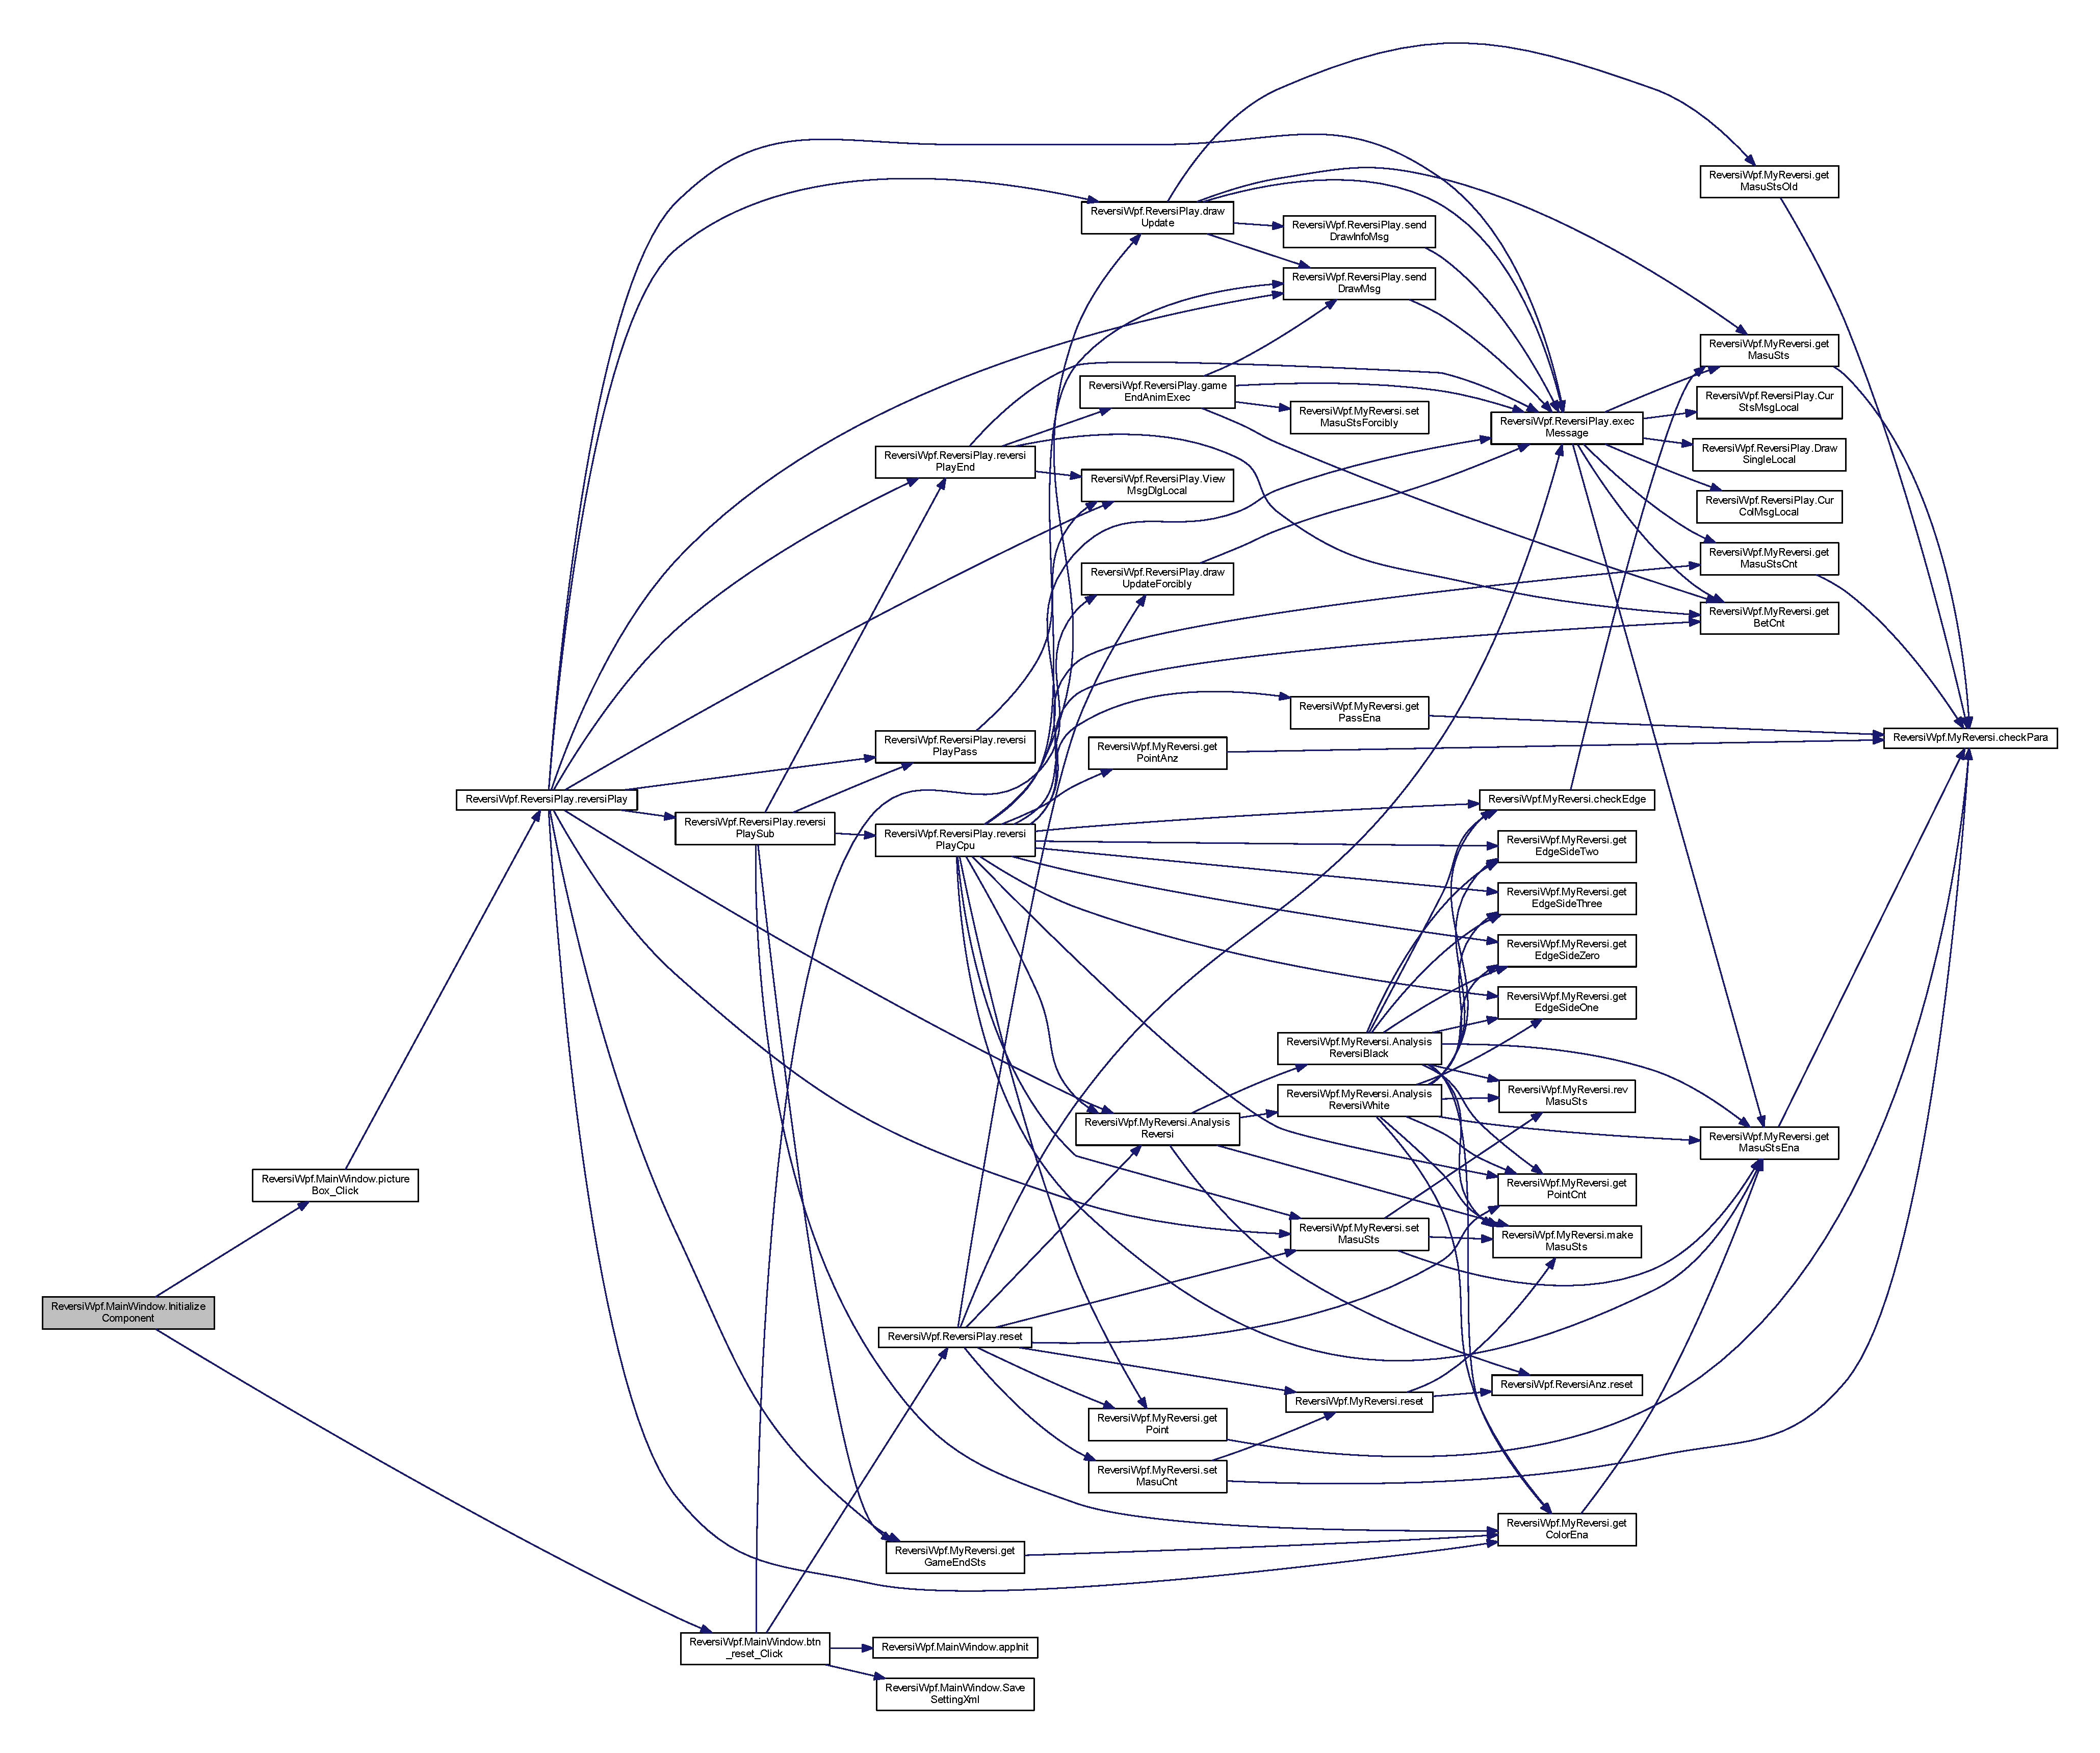
\includegraphics[width=350pt]{class_reversi_wpf_1_1_main_window_a4cf9bc92cee02fa8e3b00fa56fb41c82_cgraph}
\end{center}
\end{figure}
\mbox{\Hypertarget{class_reversi_wpf_1_1_main_window_ad911eb50aa81ec46e9f1032f264ee483}\label{class_reversi_wpf_1_1_main_window_ad911eb50aa81ec46e9f1032f264ee483}} 
\index{Reversi\+Wpf\+::\+Main\+Window@{Reversi\+Wpf\+::\+Main\+Window}!Load\+Setting\+Xml@{Load\+Setting\+Xml}}
\index{Load\+Setting\+Xml@{Load\+Setting\+Xml}!Reversi\+Wpf\+::\+Main\+Window@{Reversi\+Wpf\+::\+Main\+Window}}
\subsubsection{\texorpdfstring{Load\+Setting\+Xml()}{LoadSettingXml()}}
{\footnotesize\ttfamily \hyperlink{class_reversi_wpf_1_1_reversi_setting}{Reversi\+Setting} Reversi\+Wpf.\+Main\+Window.\+Load\+Setting\+Xml (\begin{DoxyParamCaption}\item[{string}]{path }\end{DoxyParamCaption})}



設定\+X\+M\+Lファイルロード 


\begin{DoxyParams}[1]{Parameters}
\mbox{\tt in}  & {\em string} & path 設定\+X\+M\+Lファイルパス \\
\hline
\end{DoxyParams}
\begin{DoxyReturn}{Returns}
Reversi\+Settingオブジェクトインスタンス 
\end{DoxyReturn}
\begin{DoxyAuthor}{Author}
Yuta Yoshinaga 
\end{DoxyAuthor}
\begin{DoxyDate}{Date}
2017.\+10.\+20 
\end{DoxyDate}


Definition at line 131 of file Main\+Window.\+xaml.\+cs.



Referenced by Reversi\+Wpf.\+Main\+Window.\+Main\+Window().

Here is the caller graph for this function\+:
\nopagebreak
\begin{figure}[H]
\begin{center}
\leavevmode
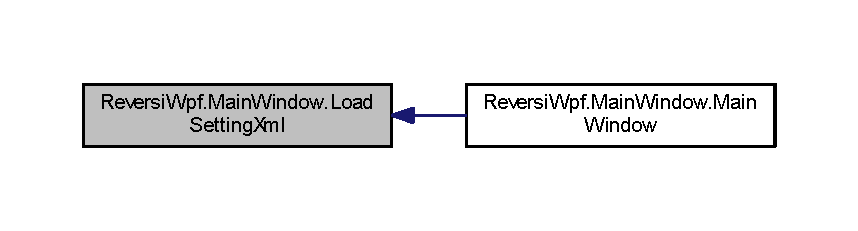
\includegraphics[width=350pt]{class_reversi_wpf_1_1_main_window_ad911eb50aa81ec46e9f1032f264ee483_icgraph}
\end{center}
\end{figure}
\mbox{\Hypertarget{class_reversi_wpf_1_1_main_window_a7514a29baed5a572e78354addb9678bc}\label{class_reversi_wpf_1_1_main_window_a7514a29baed5a572e78354addb9678bc}} 
\index{Reversi\+Wpf\+::\+Main\+Window@{Reversi\+Wpf\+::\+Main\+Window}!picture\+Box\+\_\+\+Click@{picture\+Box\+\_\+\+Click}}
\index{picture\+Box\+\_\+\+Click@{picture\+Box\+\_\+\+Click}!Reversi\+Wpf\+::\+Main\+Window@{Reversi\+Wpf\+::\+Main\+Window}}
\subsubsection{\texorpdfstring{picture\+Box\+\_\+\+Click()}{pictureBox\_Click()}}
{\footnotesize\ttfamily void Reversi\+Wpf.\+Main\+Window.\+picture\+Box\+\_\+\+Click (\begin{DoxyParamCaption}\item[{object}]{sender,  }\item[{Mouse\+Button\+Event\+Args}]{e }\end{DoxyParamCaption})\hspace{0.3cm}{\ttfamily [private]}}



マスクリック 


\begin{DoxyParams}[1]{Parameters}
\mbox{\tt in}  & {\em object} & sender \\
\hline
\mbox{\tt in}  & {\em Mouse\+Button\+Event\+Args} & e \\
\hline
\end{DoxyParams}
\begin{DoxyReturn}{Returns}
ありません 
\end{DoxyReturn}
\begin{DoxyAuthor}{Author}
Yuta Yoshinaga 
\end{DoxyAuthor}
\begin{DoxyDate}{Date}
2017.\+10.\+20 
\end{DoxyDate}


Definition at line 494 of file Main\+Window.\+xaml.\+cs.



Referenced by Reversi\+Wpf.\+Main\+Window.\+Initialize\+Component().

Here is the call graph for this function\+:
\nopagebreak
\begin{figure}[H]
\begin{center}
\leavevmode
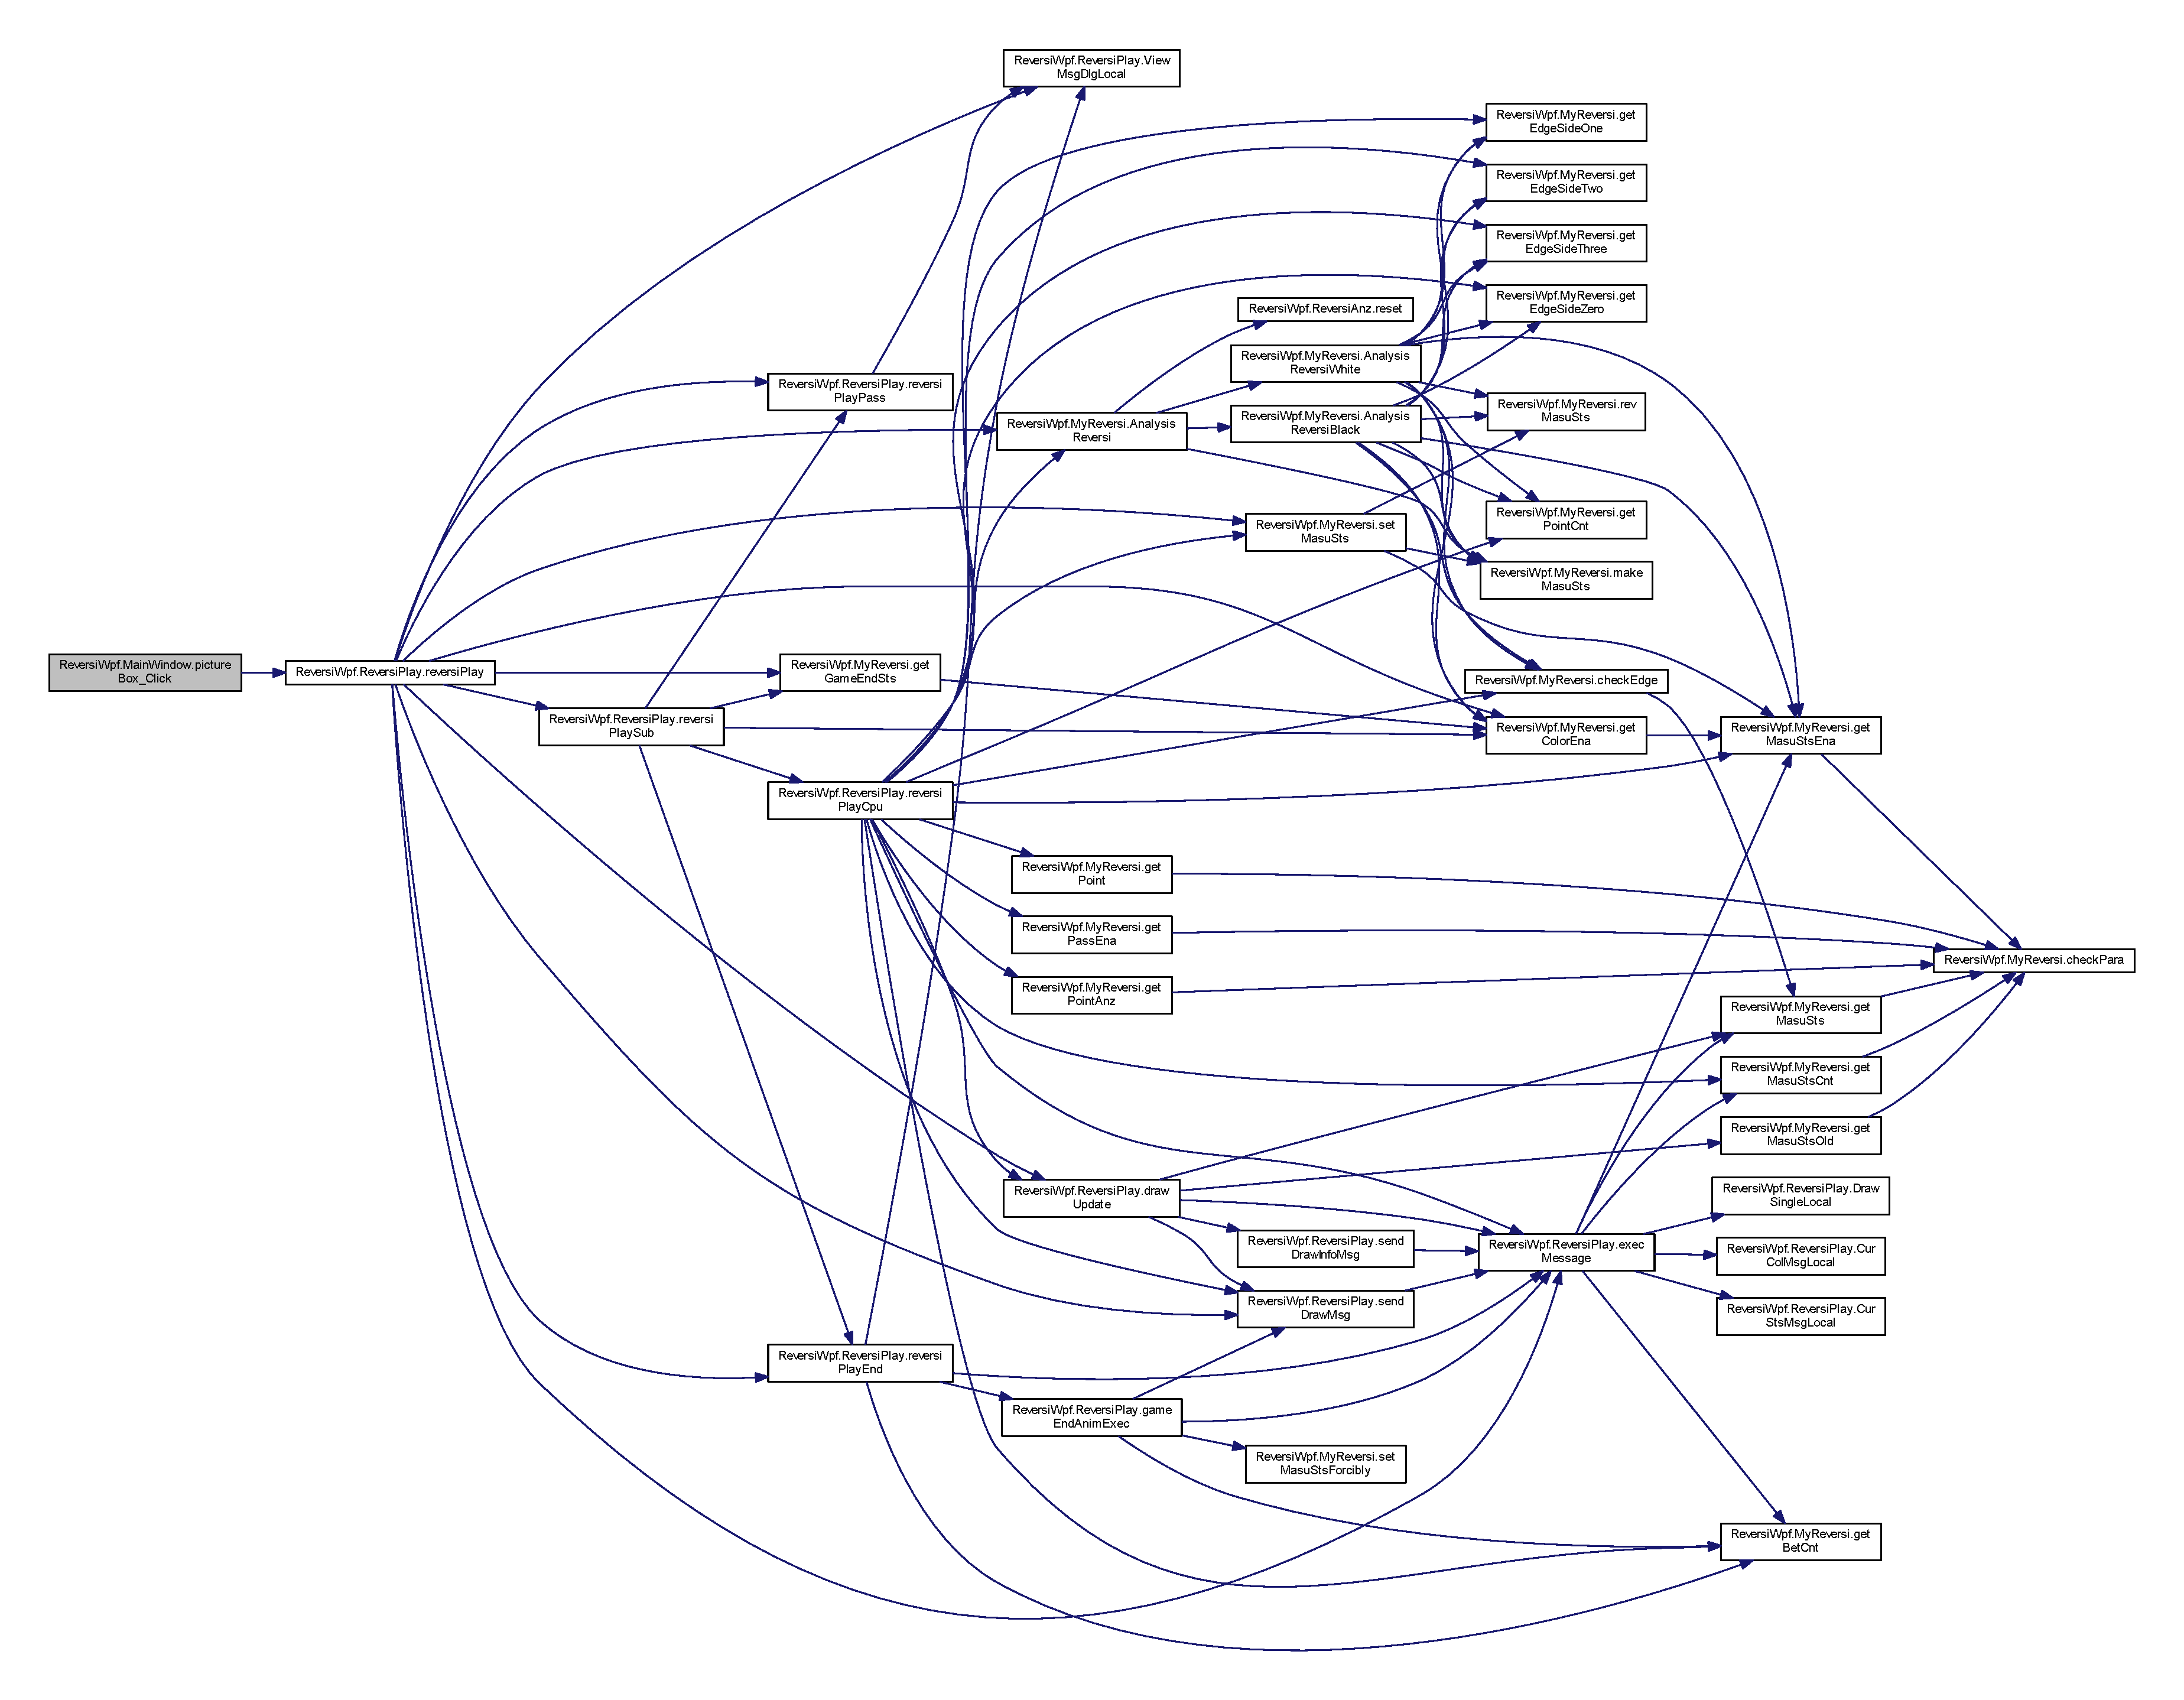
\includegraphics[width=350pt]{class_reversi_wpf_1_1_main_window_a7514a29baed5a572e78354addb9678bc_cgraph}
\end{center}
\end{figure}
Here is the caller graph for this function\+:
\nopagebreak
\begin{figure}[H]
\begin{center}
\leavevmode
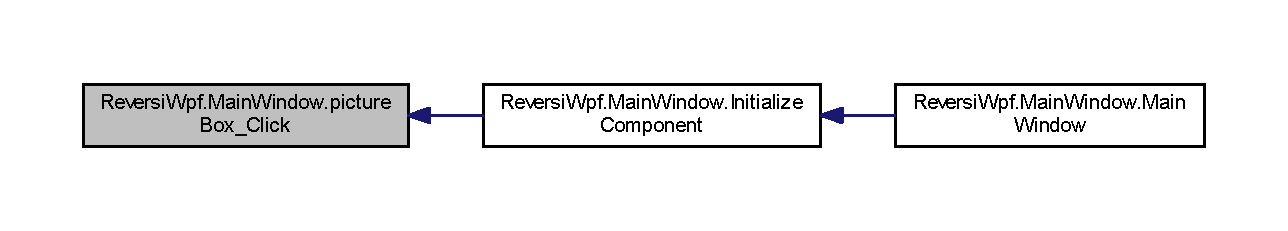
\includegraphics[width=350pt]{class_reversi_wpf_1_1_main_window_a7514a29baed5a572e78354addb9678bc_icgraph}
\end{center}
\end{figure}
\mbox{\Hypertarget{class_reversi_wpf_1_1_main_window_a02e0ae28907a572eca49167b37ce7db9}\label{class_reversi_wpf_1_1_main_window_a02e0ae28907a572eca49167b37ce7db9}} 
\index{Reversi\+Wpf\+::\+Main\+Window@{Reversi\+Wpf\+::\+Main\+Window}!Save\+Setting\+Xml@{Save\+Setting\+Xml}}
\index{Save\+Setting\+Xml@{Save\+Setting\+Xml}!Reversi\+Wpf\+::\+Main\+Window@{Reversi\+Wpf\+::\+Main\+Window}}
\subsubsection{\texorpdfstring{Save\+Setting\+Xml()}{SaveSettingXml()}}
{\footnotesize\ttfamily int Reversi\+Wpf.\+Main\+Window.\+Save\+Setting\+Xml (\begin{DoxyParamCaption}\item[{string}]{path,  }\item[{ref \hyperlink{class_reversi_wpf_1_1_reversi_setting}{Reversi\+Setting}}]{app\+Set }\end{DoxyParamCaption})}



設定\+X\+M\+Lファイルセーブ 


\begin{DoxyParams}[1]{Parameters}
\mbox{\tt in}  & {\em string} & path 設定\+X\+M\+Lファイルパス \\
\hline
\mbox{\tt out}  & {\em \hyperlink{class_reversi_wpf_1_1_reversi_setting}{Reversi\+Setting}} & app\+Set 設定\+X\+M\+Lファイルオブジェクト \\
\hline
\end{DoxyParams}
\begin{DoxyReturn}{Returns}
0 \+: 成功 それ以外 \+: 失敗 
\end{DoxyReturn}
\begin{DoxyAuthor}{Author}
Yuta Yoshinaga 
\end{DoxyAuthor}
\begin{DoxyDate}{Date}
2017.\+10.\+20 
\end{DoxyDate}


Definition at line 165 of file Main\+Window.\+xaml.\+cs.



Referenced by Reversi\+Wpf.\+Main\+Window.\+btn\+\_\+reset\+\_\+\+Click(), and Reversi\+Wpf.\+Main\+Window.\+Main\+Window().

Here is the caller graph for this function\+:
\nopagebreak
\begin{figure}[H]
\begin{center}
\leavevmode
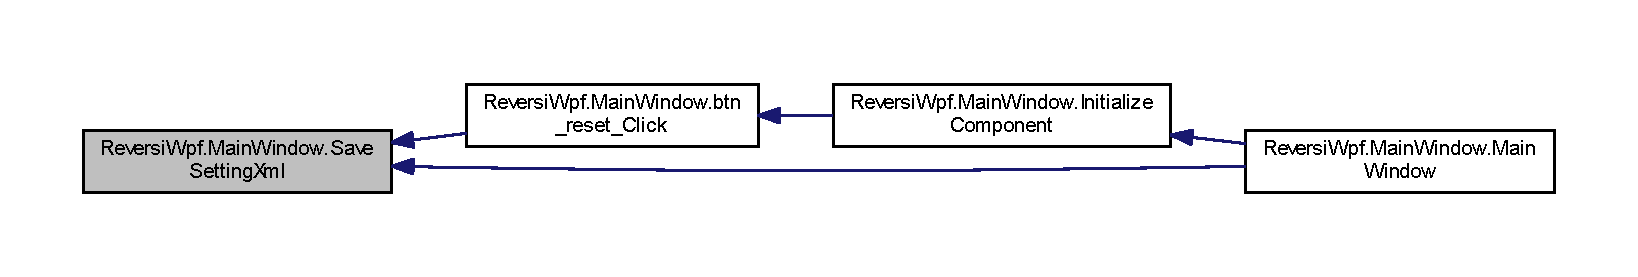
\includegraphics[width=350pt]{class_reversi_wpf_1_1_main_window_a02e0ae28907a572eca49167b37ce7db9_icgraph}
\end{center}
\end{figure}
\mbox{\Hypertarget{class_reversi_wpf_1_1_main_window_a5c093af07e7e92f21127941dff8e8684}\label{class_reversi_wpf_1_1_main_window_a5c093af07e7e92f21127941dff8e8684}} 
\index{Reversi\+Wpf\+::\+Main\+Window@{Reversi\+Wpf\+::\+Main\+Window}!To\+Image\+Source@{To\+Image\+Source}}
\index{To\+Image\+Source@{To\+Image\+Source}!Reversi\+Wpf\+::\+Main\+Window@{Reversi\+Wpf\+::\+Main\+Window}}
\subsubsection{\texorpdfstring{To\+Image\+Source()}{ToImageSource()}}
{\footnotesize\ttfamily Image\+Source Reversi\+Wpf.\+Main\+Window.\+To\+Image\+Source (\begin{DoxyParamCaption}\item[{Bitmap}]{bmp }\end{DoxyParamCaption})}



B\+I\+T\+M\+A\+Pか\+Image\+Sourceに変換 


\begin{DoxyParams}[1]{Parameters}
\mbox{\tt in}  & {\em Bitmap} & bmp \\
\hline
\end{DoxyParams}
\begin{DoxyReturn}{Returns}
Image\+Source 
\end{DoxyReturn}
\begin{DoxyAuthor}{Author}
Yuta Yoshinaga 
\end{DoxyAuthor}
\begin{DoxyDate}{Date}
2017.\+10.\+20 
\end{DoxyDate}


Definition at line 112 of file Main\+Window.\+xaml.\+cs.



Referenced by Reversi\+Wpf.\+Main\+Window.\+Draw\+Single\+Local().

Here is the call graph for this function\+:
\nopagebreak
\begin{figure}[H]
\begin{center}
\leavevmode
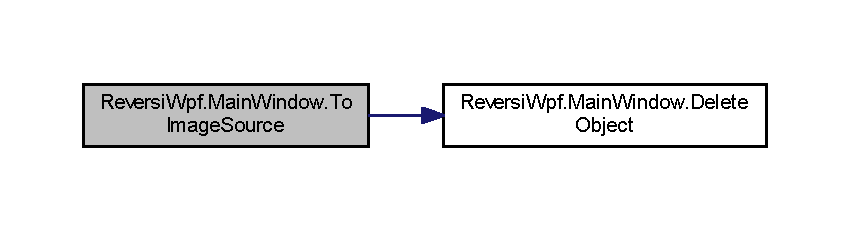
\includegraphics[width=350pt]{class_reversi_wpf_1_1_main_window_a5c093af07e7e92f21127941dff8e8684_cgraph}
\end{center}
\end{figure}
Here is the caller graph for this function\+:
\nopagebreak
\begin{figure}[H]
\begin{center}
\leavevmode
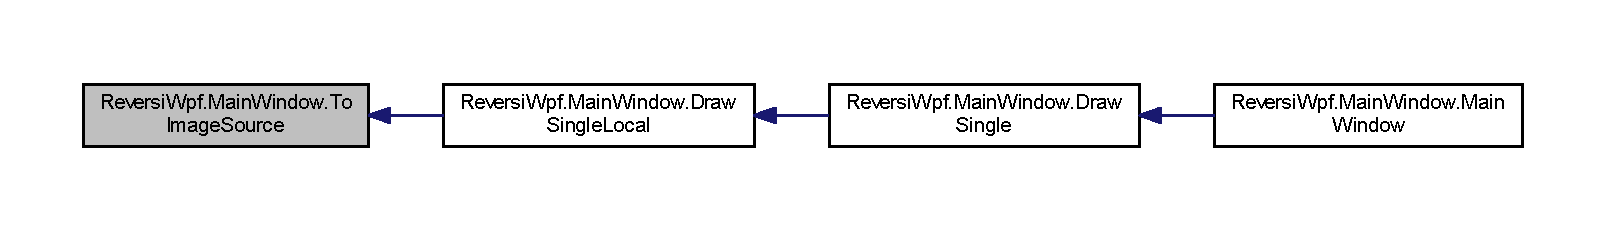
\includegraphics[width=350pt]{class_reversi_wpf_1_1_main_window_a5c093af07e7e92f21127941dff8e8684_icgraph}
\end{center}
\end{figure}
\mbox{\Hypertarget{class_reversi_wpf_1_1_main_window_aa776c697ed89869c9799576f2f6022b9}\label{class_reversi_wpf_1_1_main_window_aa776c697ed89869c9799576f2f6022b9}} 
\index{Reversi\+Wpf\+::\+Main\+Window@{Reversi\+Wpf\+::\+Main\+Window}!View\+Msg\+Dlg@{View\+Msg\+Dlg}}
\index{View\+Msg\+Dlg@{View\+Msg\+Dlg}!Reversi\+Wpf\+::\+Main\+Window@{Reversi\+Wpf\+::\+Main\+Window}}
\subsubsection{\texorpdfstring{View\+Msg\+Dlg()}{ViewMsgDlg()}}
{\footnotesize\ttfamily void Reversi\+Wpf.\+Main\+Window.\+View\+Msg\+Dlg (\begin{DoxyParamCaption}\item[{string}]{title,  }\item[{string}]{msg }\end{DoxyParamCaption})}



メッセージダイアログ 


\begin{DoxyParams}[1]{Parameters}
\mbox{\tt in}  & {\em string} & title タイトル \\
\hline
\mbox{\tt in}  & {\em string} & msg メッセージ \\
\hline
\end{DoxyParams}
\begin{DoxyReturn}{Returns}
ありません 
\end{DoxyReturn}
\begin{DoxyAuthor}{Author}
Yuta Yoshinaga 
\end{DoxyAuthor}
\begin{DoxyDate}{Date}
2017.\+10.\+20 
\end{DoxyDate}


Definition at line 265 of file Main\+Window.\+xaml.\+cs.



Referenced by Reversi\+Wpf.\+Main\+Window.\+Main\+Window().

Here is the call graph for this function\+:
\nopagebreak
\begin{figure}[H]
\begin{center}
\leavevmode
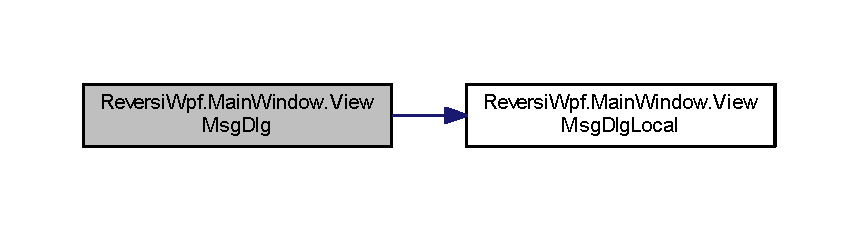
\includegraphics[width=350pt]{class_reversi_wpf_1_1_main_window_aa776c697ed89869c9799576f2f6022b9_cgraph}
\end{center}
\end{figure}
Here is the caller graph for this function\+:
\nopagebreak
\begin{figure}[H]
\begin{center}
\leavevmode
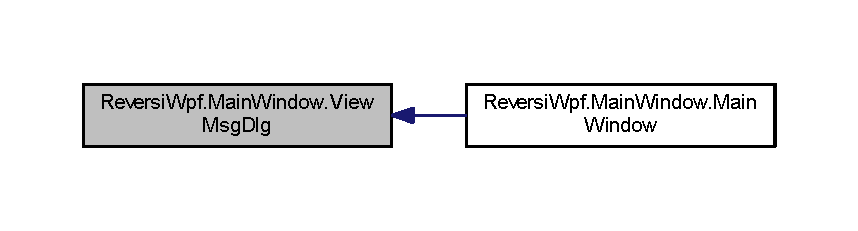
\includegraphics[width=350pt]{class_reversi_wpf_1_1_main_window_aa776c697ed89869c9799576f2f6022b9_icgraph}
\end{center}
\end{figure}
\mbox{\Hypertarget{class_reversi_wpf_1_1_main_window_a3095c98dbf6fcd1f738354a06797beb1}\label{class_reversi_wpf_1_1_main_window_a3095c98dbf6fcd1f738354a06797beb1}} 
\index{Reversi\+Wpf\+::\+Main\+Window@{Reversi\+Wpf\+::\+Main\+Window}!View\+Msg\+Dlg\+Local@{View\+Msg\+Dlg\+Local}}
\index{View\+Msg\+Dlg\+Local@{View\+Msg\+Dlg\+Local}!Reversi\+Wpf\+::\+Main\+Window@{Reversi\+Wpf\+::\+Main\+Window}}
\subsubsection{\texorpdfstring{View\+Msg\+Dlg\+Local()}{ViewMsgDlgLocal()}}
{\footnotesize\ttfamily void Reversi\+Wpf.\+Main\+Window.\+View\+Msg\+Dlg\+Local (\begin{DoxyParamCaption}\item[{string}]{title,  }\item[{string}]{msg }\end{DoxyParamCaption})}



メッセージダイアログ 


\begin{DoxyParams}[1]{Parameters}
\mbox{\tt in}  & {\em string} & title タイトル \\
\hline
\mbox{\tt in}  & {\em string} & msg メッセージ \\
\hline
\end{DoxyParams}
\begin{DoxyReturn}{Returns}
ありません 
\end{DoxyReturn}
\begin{DoxyAuthor}{Author}
Yuta Yoshinaga 
\end{DoxyAuthor}
\begin{DoxyDate}{Date}
2017.\+10.\+20 
\end{DoxyDate}


Definition at line 280 of file Main\+Window.\+xaml.\+cs.



Referenced by Reversi\+Wpf.\+Main\+Window.\+View\+Msg\+Dlg().

Here is the caller graph for this function\+:
\nopagebreak
\begin{figure}[H]
\begin{center}
\leavevmode
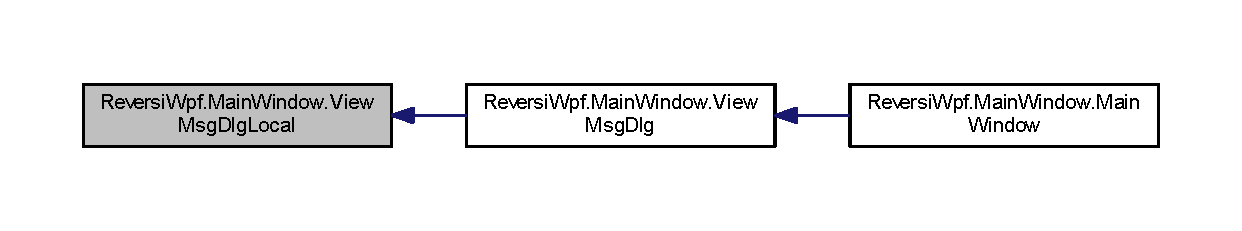
\includegraphics[width=350pt]{class_reversi_wpf_1_1_main_window_a3095c98dbf6fcd1f738354a06797beb1_icgraph}
\end{center}
\end{figure}


The documentation for this class was generated from the following files\+:\begin{DoxyCompactItemize}
\item 
\hyperlink{_main_window_8xaml_8cs}{Main\+Window.\+xaml.\+cs}\item 
obj/\+Debug/Main\+Window.\+g.\+cs\item 
obj/\+Debug/Main\+Window.\+g.\+i.\+cs\end{DoxyCompactItemize}

\hypertarget{class_reversi_wpf_1_1_my_reversi}{}\section{Reversi\+Wpf.\+My\+Reversi Class Reference}
\label{class_reversi_wpf_1_1_my_reversi}\index{Reversi\+Wpf.\+My\+Reversi@{Reversi\+Wpf.\+My\+Reversi}}


リバーシクラス  




Collaboration diagram for Reversi\+Wpf.\+My\+Reversi\+:
\nopagebreak
\begin{figure}[H]
\begin{center}
\leavevmode
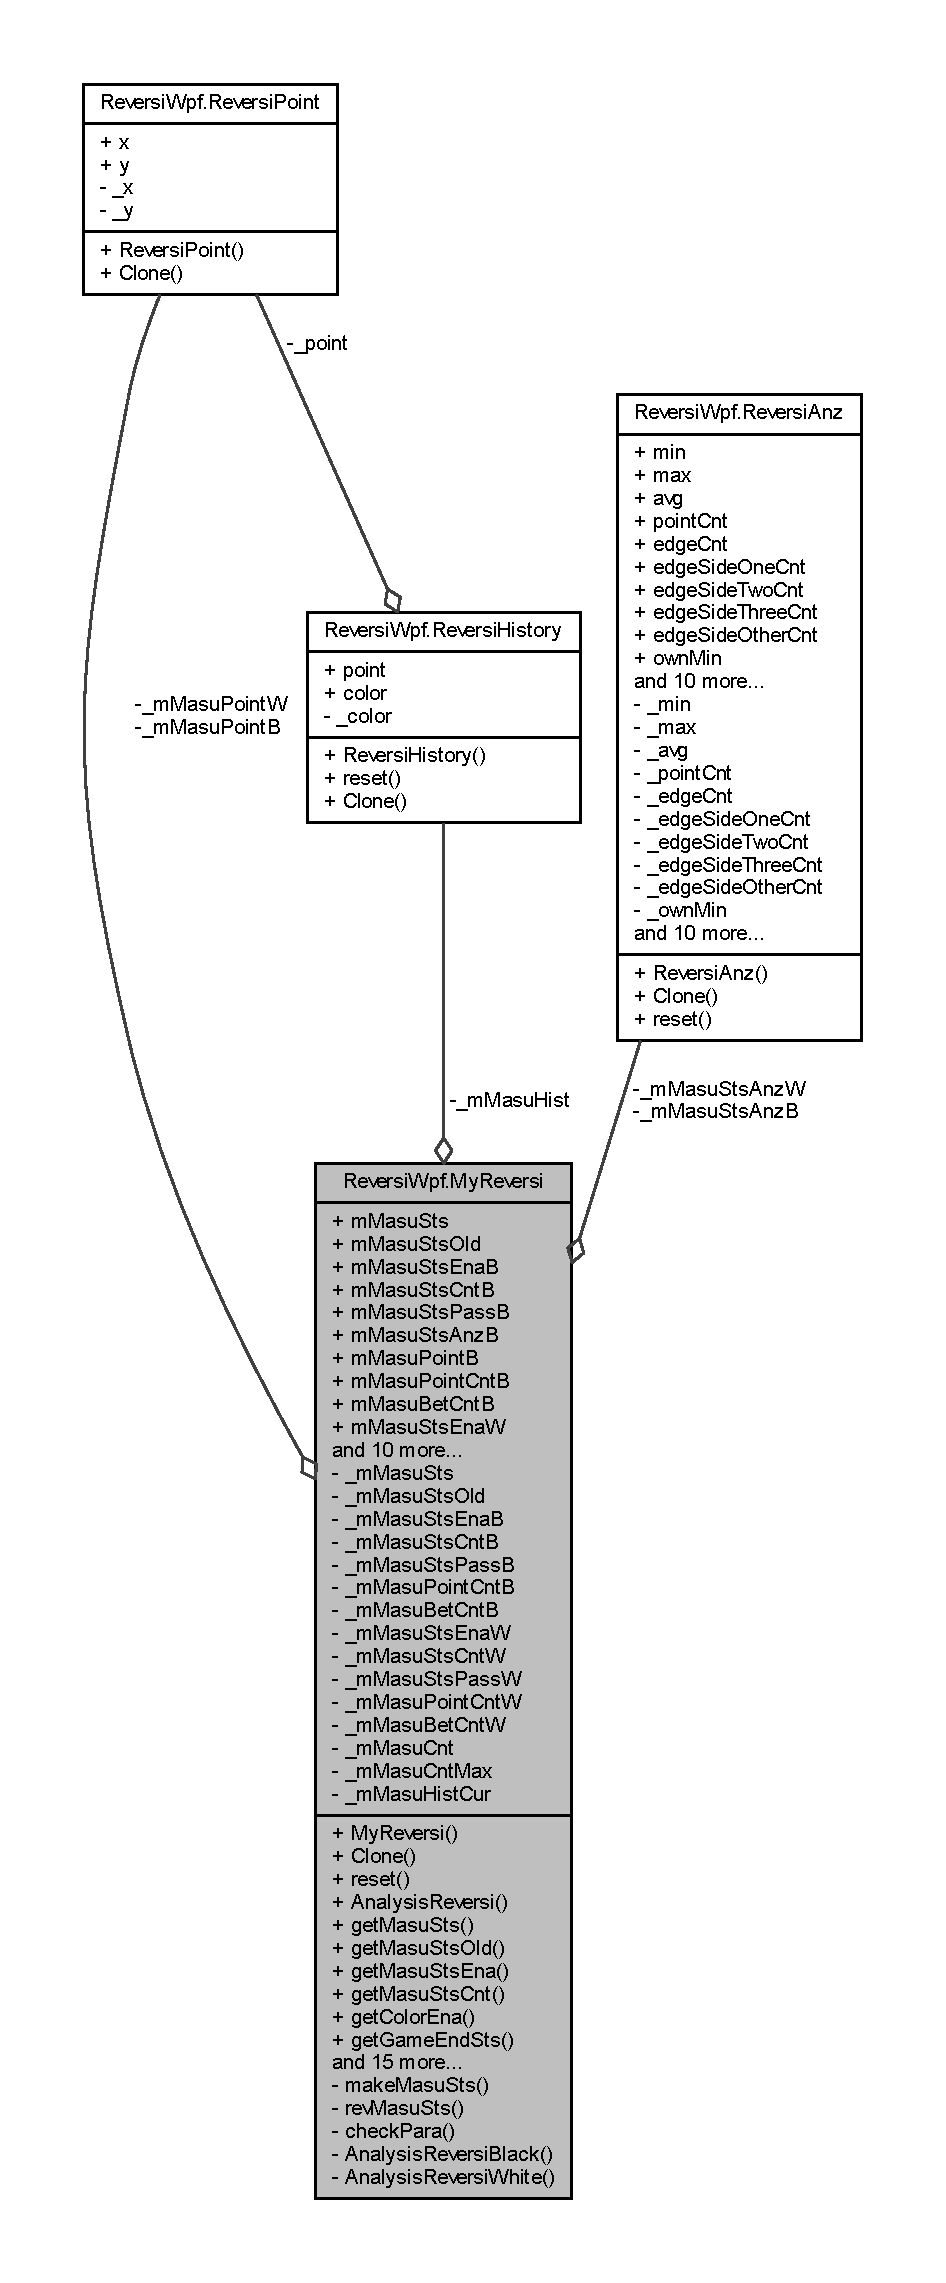
\includegraphics[height=550pt]{class_reversi_wpf_1_1_my_reversi__coll__graph}
\end{center}
\end{figure}
\subsection*{Public Member Functions}
\begin{DoxyCompactItemize}
\item 
\hyperlink{class_reversi_wpf_1_1_my_reversi_aff9b8ea39ef41f0d0b84cc5d52af86b2}{My\+Reversi} (int masu\+Cnt, int masu\+Max)
\begin{DoxyCompactList}\small\item\em コンストラクタ \end{DoxyCompactList}\item 
\hyperlink{class_reversi_wpf_1_1_my_reversi}{My\+Reversi} \hyperlink{class_reversi_wpf_1_1_my_reversi_aff9b97e9e4102966ea558428255974e2}{Clone} ()
\begin{DoxyCompactList}\small\item\em コピー \end{DoxyCompactList}\item 
void \hyperlink{class_reversi_wpf_1_1_my_reversi_a61b1ee2e28cc4050ebbda2e54c7a60b6}{reset} ()
\begin{DoxyCompactList}\small\item\em リセット \end{DoxyCompactList}\item 
void \hyperlink{class_reversi_wpf_1_1_my_reversi_a14a3c0720db3ff11196e0c7c34bd80c0}{Analysis\+Reversi} (int b\+Pass\+Ena, int w\+Pass\+Ena)
\begin{DoxyCompactList}\small\item\em 解析を行う \end{DoxyCompactList}\item 
int \hyperlink{class_reversi_wpf_1_1_my_reversi_a34b0c0b96b147a8d2f1dc6863cac25d8}{get\+Masu\+Sts} (int y, int x)
\begin{DoxyCompactList}\small\item\em マスステータスを取得 \end{DoxyCompactList}\item 
int \hyperlink{class_reversi_wpf_1_1_my_reversi_acdf94f106c88ded99a4c5dcbbc19be16}{get\+Masu\+Sts\+Old} (int y, int x)
\begin{DoxyCompactList}\small\item\em 以前のマスステータスを取得 \end{DoxyCompactList}\item 
int \hyperlink{class_reversi_wpf_1_1_my_reversi_ac122d3db633616259d22d8bb885c074d}{get\+Masu\+Sts\+Ena} (int color, int y, int x)
\begin{DoxyCompactList}\small\item\em 指定座標に指定色を置けるかチェック \end{DoxyCompactList}\item 
int \hyperlink{class_reversi_wpf_1_1_my_reversi_ac2723c418d4b51ec0e4598cbd44634f0}{get\+Masu\+Sts\+Cnt} (int color, int y, int x)
\begin{DoxyCompactList}\small\item\em 指定座標の獲得コマ数取得 \end{DoxyCompactList}\item 
int \hyperlink{class_reversi_wpf_1_1_my_reversi_a9a7c386e4b5007a937865ab301774c9e}{get\+Color\+Ena} (int color)
\begin{DoxyCompactList}\small\item\em 指定色が現在置ける場所があるかチェック \end{DoxyCompactList}\item 
int \hyperlink{class_reversi_wpf_1_1_my_reversi_a77a81c9c08a6dadcab0dd5741de1b88b}{get\+Game\+End\+Sts} ()
\begin{DoxyCompactList}\small\item\em ゲーム終了かチェック \end{DoxyCompactList}\item 
int \hyperlink{class_reversi_wpf_1_1_my_reversi_a03c7e639718936243e30302680c63f99}{set\+Masu\+Sts} (int color, int y, int x)
\begin{DoxyCompactList}\small\item\em 指定座標にコマを置く \end{DoxyCompactList}\item 
int \hyperlink{class_reversi_wpf_1_1_my_reversi_a6526ef12950147cd9900e0c2f8a33f1c}{set\+Masu\+Sts\+Forcibly} (int color, int y, int x)
\begin{DoxyCompactList}\small\item\em 指定座標にコマを強制的に置く \end{DoxyCompactList}\item 
int \hyperlink{class_reversi_wpf_1_1_my_reversi_a1e25c6ee30dd15b6ae87e355bddd6af6}{set\+Masu\+Cnt} (int cnt)
\begin{DoxyCompactList}\small\item\em マスの数変更 \end{DoxyCompactList}\item 
\hyperlink{class_reversi_wpf_1_1_reversi_point}{Reversi\+Point} \hyperlink{class_reversi_wpf_1_1_my_reversi_a4e31d8df5c6759c2f6afea00f8332706}{get\+Point} (int color, int num)
\begin{DoxyCompactList}\small\item\em ポイント座標取得 \end{DoxyCompactList}\item 
int \hyperlink{class_reversi_wpf_1_1_my_reversi_a86f08f7b19fe00b88ef7236bd784a451}{get\+Point\+Cnt} (int color)
\begin{DoxyCompactList}\small\item\em ポイント座標数取得 \end{DoxyCompactList}\item 
int \hyperlink{class_reversi_wpf_1_1_my_reversi_a57482d7118dad2c5d104e186acd5212b}{get\+Bet\+Cnt} (int color)
\begin{DoxyCompactList}\small\item\em コマ数取得 \end{DoxyCompactList}\item 
int \hyperlink{class_reversi_wpf_1_1_my_reversi_ab450b1508d0190909b016ed1855905e3}{get\+Pass\+Ena} (int color, int y, int x)
\begin{DoxyCompactList}\small\item\em パス判定 \end{DoxyCompactList}\item 
\hyperlink{class_reversi_wpf_1_1_reversi_history}{Reversi\+History} \hyperlink{class_reversi_wpf_1_1_my_reversi_aa85fcb151ab7c188b0637b9eb9269baa}{get\+History} (int num)
\begin{DoxyCompactList}\small\item\em 履歴取得 \end{DoxyCompactList}\item 
int \hyperlink{class_reversi_wpf_1_1_my_reversi_a9e6ba44101405de13825f3585fda00af}{get\+History\+Cnt} ()
\begin{DoxyCompactList}\small\item\em 履歴数取得 \end{DoxyCompactList}\item 
\hyperlink{class_reversi_wpf_1_1_reversi_anz}{Reversi\+Anz} \hyperlink{class_reversi_wpf_1_1_my_reversi_af60c852859185c303ebd4d9b5b3f8700}{get\+Point\+Anz} (int color, int y, int x)
\begin{DoxyCompactList}\small\item\em ポイント座標解析取得 \end{DoxyCompactList}\item 
int \hyperlink{class_reversi_wpf_1_1_my_reversi_acad9426b5389a91f1f42c733b2f2097e}{check\+Edge} (int color, int y, int x)
\begin{DoxyCompactList}\small\item\em 角の隣に置いても角を取られないマス検索 \end{DoxyCompactList}\item 
int \hyperlink{class_reversi_wpf_1_1_my_reversi_a3418fce34fd194987dc0efcd7aa654a4}{get\+Edge\+Side\+Zero} (int y, int x)
\begin{DoxyCompactList}\small\item\em 指定座標が角か取得 \end{DoxyCompactList}\item 
int \hyperlink{class_reversi_wpf_1_1_my_reversi_a6e9641216f52b0c384f43a26cfea981f}{get\+Edge\+Side\+One} (int y, int x)
\begin{DoxyCompactList}\small\item\em 指定座標が角の一つ手前か取得 \end{DoxyCompactList}\item 
int \hyperlink{class_reversi_wpf_1_1_my_reversi_ae59ceaeded22519213df314ab31b45d1}{get\+Edge\+Side\+Two} (int y, int x)
\begin{DoxyCompactList}\small\item\em 指定座標が角の二つ手前か取得 \end{DoxyCompactList}\item 
int \hyperlink{class_reversi_wpf_1_1_my_reversi_a278da279bc20775b0849a1316729d6a3}{get\+Edge\+Side\+Three} (int y, int x)
\begin{DoxyCompactList}\small\item\em 指定座標が角の三つ以上手前か取得 \end{DoxyCompactList}\end{DoxyCompactItemize}
\subsection*{Properties}
\begin{DoxyCompactItemize}
\item 
\mbox{\Hypertarget{class_reversi_wpf_1_1_my_reversi_a614013530cef0e862694940302699a65}\label{class_reversi_wpf_1_1_my_reversi_a614013530cef0e862694940302699a65}} 
int \mbox{[},\mbox{]} {\bfseries m\+Masu\+Sts}\hspace{0.3cm}{\ttfamily  \mbox{[}get, set\mbox{]}}
\item 
\mbox{\Hypertarget{class_reversi_wpf_1_1_my_reversi_a7a99f1b8317de2c66ed8df8be1937498}\label{class_reversi_wpf_1_1_my_reversi_a7a99f1b8317de2c66ed8df8be1937498}} 
int \mbox{[},\mbox{]} {\bfseries m\+Masu\+Sts\+Old}\hspace{0.3cm}{\ttfamily  \mbox{[}get, set\mbox{]}}
\item 
\mbox{\Hypertarget{class_reversi_wpf_1_1_my_reversi_a41c8fd6eee0e15ec93ce51b1b862a966}\label{class_reversi_wpf_1_1_my_reversi_a41c8fd6eee0e15ec93ce51b1b862a966}} 
int \mbox{[},\mbox{]} {\bfseries m\+Masu\+Sts\+EnaB}\hspace{0.3cm}{\ttfamily  \mbox{[}get, set\mbox{]}}
\item 
\mbox{\Hypertarget{class_reversi_wpf_1_1_my_reversi_a3c302cf1c6ba2326cadb61103d1a0d0a}\label{class_reversi_wpf_1_1_my_reversi_a3c302cf1c6ba2326cadb61103d1a0d0a}} 
int \mbox{[},\mbox{]} {\bfseries m\+Masu\+Sts\+CntB}\hspace{0.3cm}{\ttfamily  \mbox{[}get, set\mbox{]}}
\item 
\mbox{\Hypertarget{class_reversi_wpf_1_1_my_reversi_a0eb19d7494fec60688bc75c8f9d84b21}\label{class_reversi_wpf_1_1_my_reversi_a0eb19d7494fec60688bc75c8f9d84b21}} 
int \mbox{[},\mbox{]} {\bfseries m\+Masu\+Sts\+PassB}\hspace{0.3cm}{\ttfamily  \mbox{[}get, set\mbox{]}}
\item 
\mbox{\Hypertarget{class_reversi_wpf_1_1_my_reversi_ad527994d0f3aa68d75214215c3addfee}\label{class_reversi_wpf_1_1_my_reversi_ad527994d0f3aa68d75214215c3addfee}} 
\hyperlink{class_reversi_wpf_1_1_reversi_anz}{Reversi\+Anz} \mbox{[},\mbox{]} {\bfseries m\+Masu\+Sts\+AnzB}\hspace{0.3cm}{\ttfamily  \mbox{[}get, set\mbox{]}}
\item 
\mbox{\Hypertarget{class_reversi_wpf_1_1_my_reversi_a79df02cb50ee3f939d31c72da66a7b87}\label{class_reversi_wpf_1_1_my_reversi_a79df02cb50ee3f939d31c72da66a7b87}} 
\hyperlink{class_reversi_wpf_1_1_reversi_point}{Reversi\+Point} \mbox{[}$\,$\mbox{]} {\bfseries m\+Masu\+PointB}\hspace{0.3cm}{\ttfamily  \mbox{[}get, set\mbox{]}}
\item 
\mbox{\Hypertarget{class_reversi_wpf_1_1_my_reversi_abdbf1a6370b27ca1cbbe9a16f235c005}\label{class_reversi_wpf_1_1_my_reversi_abdbf1a6370b27ca1cbbe9a16f235c005}} 
int {\bfseries m\+Masu\+Point\+CntB}\hspace{0.3cm}{\ttfamily  \mbox{[}get, set\mbox{]}}
\item 
\mbox{\Hypertarget{class_reversi_wpf_1_1_my_reversi_ad868ac31d1b755a05723310096b03d35}\label{class_reversi_wpf_1_1_my_reversi_ad868ac31d1b755a05723310096b03d35}} 
int {\bfseries m\+Masu\+Bet\+CntB}\hspace{0.3cm}{\ttfamily  \mbox{[}get, set\mbox{]}}
\item 
\mbox{\Hypertarget{class_reversi_wpf_1_1_my_reversi_a32298d802e922dd5d343b8fcfc4642e5}\label{class_reversi_wpf_1_1_my_reversi_a32298d802e922dd5d343b8fcfc4642e5}} 
int \mbox{[},\mbox{]} {\bfseries m\+Masu\+Sts\+EnaW}\hspace{0.3cm}{\ttfamily  \mbox{[}get, set\mbox{]}}
\item 
\mbox{\Hypertarget{class_reversi_wpf_1_1_my_reversi_a56ec98f5218f623f1ee91ce4d5468556}\label{class_reversi_wpf_1_1_my_reversi_a56ec98f5218f623f1ee91ce4d5468556}} 
int \mbox{[},\mbox{]} {\bfseries m\+Masu\+Sts\+CntW}\hspace{0.3cm}{\ttfamily  \mbox{[}get, set\mbox{]}}
\item 
\mbox{\Hypertarget{class_reversi_wpf_1_1_my_reversi_ab9b583094662b088deb0cb2af567e07f}\label{class_reversi_wpf_1_1_my_reversi_ab9b583094662b088deb0cb2af567e07f}} 
int \mbox{[},\mbox{]} {\bfseries m\+Masu\+Sts\+PassW}\hspace{0.3cm}{\ttfamily  \mbox{[}get, set\mbox{]}}
\item 
\mbox{\Hypertarget{class_reversi_wpf_1_1_my_reversi_a227de3b978b1d13c38441bfe26e98133}\label{class_reversi_wpf_1_1_my_reversi_a227de3b978b1d13c38441bfe26e98133}} 
\hyperlink{class_reversi_wpf_1_1_reversi_anz}{Reversi\+Anz} \mbox{[},\mbox{]} {\bfseries m\+Masu\+Sts\+AnzW}\hspace{0.3cm}{\ttfamily  \mbox{[}get, set\mbox{]}}
\item 
\mbox{\Hypertarget{class_reversi_wpf_1_1_my_reversi_a7ec02263060bea6af746df22af1208c9}\label{class_reversi_wpf_1_1_my_reversi_a7ec02263060bea6af746df22af1208c9}} 
\hyperlink{class_reversi_wpf_1_1_reversi_point}{Reversi\+Point} \mbox{[}$\,$\mbox{]} {\bfseries m\+Masu\+PointW}\hspace{0.3cm}{\ttfamily  \mbox{[}get, set\mbox{]}}
\item 
\mbox{\Hypertarget{class_reversi_wpf_1_1_my_reversi_abf928720667c1322ddf923ff7306d646}\label{class_reversi_wpf_1_1_my_reversi_abf928720667c1322ddf923ff7306d646}} 
int {\bfseries m\+Masu\+Point\+CntW}\hspace{0.3cm}{\ttfamily  \mbox{[}get, set\mbox{]}}
\item 
\mbox{\Hypertarget{class_reversi_wpf_1_1_my_reversi_ac71fbd0b44f0045c61b3951737b405b3}\label{class_reversi_wpf_1_1_my_reversi_ac71fbd0b44f0045c61b3951737b405b3}} 
int {\bfseries m\+Masu\+Bet\+CntW}\hspace{0.3cm}{\ttfamily  \mbox{[}get, set\mbox{]}}
\item 
\mbox{\Hypertarget{class_reversi_wpf_1_1_my_reversi_a6b594447d9192ef63ad3dbd7f1fd151e}\label{class_reversi_wpf_1_1_my_reversi_a6b594447d9192ef63ad3dbd7f1fd151e}} 
int {\bfseries m\+Masu\+Cnt}\hspace{0.3cm}{\ttfamily  \mbox{[}get, set\mbox{]}}
\item 
\mbox{\Hypertarget{class_reversi_wpf_1_1_my_reversi_a245415a7553513696470775bfb7d0417}\label{class_reversi_wpf_1_1_my_reversi_a245415a7553513696470775bfb7d0417}} 
int {\bfseries m\+Masu\+Cnt\+Max}\hspace{0.3cm}{\ttfamily  \mbox{[}get, set\mbox{]}}
\item 
\mbox{\Hypertarget{class_reversi_wpf_1_1_my_reversi_aa9b49dcd3db0f27f99d845801cfed03c}\label{class_reversi_wpf_1_1_my_reversi_aa9b49dcd3db0f27f99d845801cfed03c}} 
int {\bfseries m\+Masu\+Hist\+Cur}\hspace{0.3cm}{\ttfamily  \mbox{[}get, set\mbox{]}}
\item 
\mbox{\Hypertarget{class_reversi_wpf_1_1_my_reversi_a904bd26199f9961eff0b8ac999db8f34}\label{class_reversi_wpf_1_1_my_reversi_a904bd26199f9961eff0b8ac999db8f34}} 
\hyperlink{class_reversi_wpf_1_1_reversi_history}{Reversi\+History} \mbox{[}$\,$\mbox{]} {\bfseries m\+Masu\+Hist}\hspace{0.3cm}{\ttfamily  \mbox{[}get, set\mbox{]}}
\end{DoxyCompactItemize}
\subsection*{Private Member Functions}
\begin{DoxyCompactItemize}
\item 
int \hyperlink{class_reversi_wpf_1_1_my_reversi_a7e4d94600afb1b9d512341b1692769e7}{make\+Masu\+Sts} (int color)
\begin{DoxyCompactList}\small\item\em 各コマの置ける場所等のステータス作成 \end{DoxyCompactList}\item 
void \hyperlink{class_reversi_wpf_1_1_my_reversi_a0c99040662eebcca741bdda303f07eb6}{rev\+Masu\+Sts} (int color, int y, int x)
\begin{DoxyCompactList}\small\item\em コマをひっくり返す \end{DoxyCompactList}\item 
int \hyperlink{class_reversi_wpf_1_1_my_reversi_adc98d24744c8e50f62f94b9441f582c5}{check\+Para} (int para, int min, int max)
\begin{DoxyCompactList}\small\item\em パラメーター範囲チェック \end{DoxyCompactList}\item 
void \hyperlink{class_reversi_wpf_1_1_my_reversi_af7ca68ea9f05d79c1debbdc320555098}{Analysis\+Reversi\+Black} ()
\begin{DoxyCompactList}\small\item\em 解析を行う(黒) \end{DoxyCompactList}\item 
void \hyperlink{class_reversi_wpf_1_1_my_reversi_a7be281b0dbae11afb652260b4d30f128}{Analysis\+Reversi\+White} ()
\begin{DoxyCompactList}\small\item\em 解析を行う(白) \end{DoxyCompactList}\end{DoxyCompactItemize}
\subsection*{Private Attributes}
\begin{DoxyCompactItemize}
\item 
\mbox{\Hypertarget{class_reversi_wpf_1_1_my_reversi_a4163f1fa653867301cb63221f5ae3461}\label{class_reversi_wpf_1_1_my_reversi_a4163f1fa653867301cb63221f5ae3461}} 
int \mbox{[},\mbox{]} \hyperlink{class_reversi_wpf_1_1_my_reversi_a4163f1fa653867301cb63221f5ae3461}{\+\_\+m\+Masu\+Sts}
\begin{DoxyCompactList}\small\item\em マスの状態 \end{DoxyCompactList}\item 
\mbox{\Hypertarget{class_reversi_wpf_1_1_my_reversi_a9cb2e9ec7e6a3361508003e41283f2ad}\label{class_reversi_wpf_1_1_my_reversi_a9cb2e9ec7e6a3361508003e41283f2ad}} 
int \mbox{[},\mbox{]} \hyperlink{class_reversi_wpf_1_1_my_reversi_a9cb2e9ec7e6a3361508003e41283f2ad}{\+\_\+m\+Masu\+Sts\+Old}
\begin{DoxyCompactList}\small\item\em 以前のマスの状態 \end{DoxyCompactList}\item 
\mbox{\Hypertarget{class_reversi_wpf_1_1_my_reversi_a40b4d1e5946dbf7ee1af76ab66d5564a}\label{class_reversi_wpf_1_1_my_reversi_a40b4d1e5946dbf7ee1af76ab66d5564a}} 
int \mbox{[},\mbox{]} \hyperlink{class_reversi_wpf_1_1_my_reversi_a40b4d1e5946dbf7ee1af76ab66d5564a}{\+\_\+m\+Masu\+Sts\+EnaB}
\begin{DoxyCompactList}\small\item\em 黒の置ける場所 \end{DoxyCompactList}\item 
\mbox{\Hypertarget{class_reversi_wpf_1_1_my_reversi_a5b5538a3638613d4f6041b7a50a39196}\label{class_reversi_wpf_1_1_my_reversi_a5b5538a3638613d4f6041b7a50a39196}} 
int \mbox{[},\mbox{]} \hyperlink{class_reversi_wpf_1_1_my_reversi_a5b5538a3638613d4f6041b7a50a39196}{\+\_\+m\+Masu\+Sts\+CntB}
\begin{DoxyCompactList}\small\item\em 黒の獲得コマ数 \end{DoxyCompactList}\item 
\mbox{\Hypertarget{class_reversi_wpf_1_1_my_reversi_afb0fc9600af55b8a7f1b57c2f47c925b}\label{class_reversi_wpf_1_1_my_reversi_afb0fc9600af55b8a7f1b57c2f47c925b}} 
int \mbox{[},\mbox{]} \hyperlink{class_reversi_wpf_1_1_my_reversi_afb0fc9600af55b8a7f1b57c2f47c925b}{\+\_\+m\+Masu\+Sts\+PassB}
\begin{DoxyCompactList}\small\item\em 黒が相手をパスさせる場所 \end{DoxyCompactList}\item 
\mbox{\Hypertarget{class_reversi_wpf_1_1_my_reversi_ac25af444b26d15b6dd62e8cbaa37ceb1}\label{class_reversi_wpf_1_1_my_reversi_ac25af444b26d15b6dd62e8cbaa37ceb1}} 
\hyperlink{class_reversi_wpf_1_1_reversi_anz}{Reversi\+Anz} \mbox{[},\mbox{]} \hyperlink{class_reversi_wpf_1_1_my_reversi_ac25af444b26d15b6dd62e8cbaa37ceb1}{\+\_\+m\+Masu\+Sts\+AnzB}
\begin{DoxyCompactList}\small\item\em 黒がその場所に置いた場合の解析結果 \end{DoxyCompactList}\item 
\mbox{\Hypertarget{class_reversi_wpf_1_1_my_reversi_a2c5799e5b2910f655cf5fb4bd3a80c48}\label{class_reversi_wpf_1_1_my_reversi_a2c5799e5b2910f655cf5fb4bd3a80c48}} 
\hyperlink{class_reversi_wpf_1_1_reversi_point}{Reversi\+Point} \mbox{[}$\,$\mbox{]} \hyperlink{class_reversi_wpf_1_1_my_reversi_a2c5799e5b2910f655cf5fb4bd3a80c48}{\+\_\+m\+Masu\+PointB}
\begin{DoxyCompactList}\small\item\em 黒の置ける場所座標一覧 \end{DoxyCompactList}\item 
\mbox{\Hypertarget{class_reversi_wpf_1_1_my_reversi_a13697cce632f1bf85a1de1b0b9198a27}\label{class_reversi_wpf_1_1_my_reversi_a13697cce632f1bf85a1de1b0b9198a27}} 
int \hyperlink{class_reversi_wpf_1_1_my_reversi_a13697cce632f1bf85a1de1b0b9198a27}{\+\_\+m\+Masu\+Point\+CntB}
\begin{DoxyCompactList}\small\item\em 黒の置ける場所座標一覧数 \end{DoxyCompactList}\item 
\mbox{\Hypertarget{class_reversi_wpf_1_1_my_reversi_ae943daa01dd5aee6af47d99233ed16ef}\label{class_reversi_wpf_1_1_my_reversi_ae943daa01dd5aee6af47d99233ed16ef}} 
int \hyperlink{class_reversi_wpf_1_1_my_reversi_ae943daa01dd5aee6af47d99233ed16ef}{\+\_\+m\+Masu\+Bet\+CntB}
\begin{DoxyCompactList}\small\item\em 黒コマ数 \end{DoxyCompactList}\item 
\mbox{\Hypertarget{class_reversi_wpf_1_1_my_reversi_a829c8b2bddf2ef75c00694df7279d719}\label{class_reversi_wpf_1_1_my_reversi_a829c8b2bddf2ef75c00694df7279d719}} 
int \mbox{[},\mbox{]} \hyperlink{class_reversi_wpf_1_1_my_reversi_a829c8b2bddf2ef75c00694df7279d719}{\+\_\+m\+Masu\+Sts\+EnaW}
\begin{DoxyCompactList}\small\item\em 白の置ける場所 \end{DoxyCompactList}\item 
\mbox{\Hypertarget{class_reversi_wpf_1_1_my_reversi_a7b061b449d33913ff3a5c1070853e362}\label{class_reversi_wpf_1_1_my_reversi_a7b061b449d33913ff3a5c1070853e362}} 
int \mbox{[},\mbox{]} \hyperlink{class_reversi_wpf_1_1_my_reversi_a7b061b449d33913ff3a5c1070853e362}{\+\_\+m\+Masu\+Sts\+CntW}
\begin{DoxyCompactList}\small\item\em 白の獲得コマ数 \end{DoxyCompactList}\item 
\mbox{\Hypertarget{class_reversi_wpf_1_1_my_reversi_a96b0453ea035082c59361e3f6accfe2b}\label{class_reversi_wpf_1_1_my_reversi_a96b0453ea035082c59361e3f6accfe2b}} 
int \mbox{[},\mbox{]} \hyperlink{class_reversi_wpf_1_1_my_reversi_a96b0453ea035082c59361e3f6accfe2b}{\+\_\+m\+Masu\+Sts\+PassW}
\begin{DoxyCompactList}\small\item\em 白が相手をパスさせる場所 \end{DoxyCompactList}\item 
\mbox{\Hypertarget{class_reversi_wpf_1_1_my_reversi_ada90dae4eb587e21a96b89fb8df21a83}\label{class_reversi_wpf_1_1_my_reversi_ada90dae4eb587e21a96b89fb8df21a83}} 
\hyperlink{class_reversi_wpf_1_1_reversi_anz}{Reversi\+Anz} \mbox{[},\mbox{]} \hyperlink{class_reversi_wpf_1_1_my_reversi_ada90dae4eb587e21a96b89fb8df21a83}{\+\_\+m\+Masu\+Sts\+AnzW}
\begin{DoxyCompactList}\small\item\em 白がその場所に置いた場合の解析結果 \end{DoxyCompactList}\item 
\mbox{\Hypertarget{class_reversi_wpf_1_1_my_reversi_a6d7ee497538c97b0d11b09e4f0530303}\label{class_reversi_wpf_1_1_my_reversi_a6d7ee497538c97b0d11b09e4f0530303}} 
\hyperlink{class_reversi_wpf_1_1_reversi_point}{Reversi\+Point} \mbox{[}$\,$\mbox{]} \hyperlink{class_reversi_wpf_1_1_my_reversi_a6d7ee497538c97b0d11b09e4f0530303}{\+\_\+m\+Masu\+PointW}
\begin{DoxyCompactList}\small\item\em 白の置ける場所座標一覧 \end{DoxyCompactList}\item 
\mbox{\Hypertarget{class_reversi_wpf_1_1_my_reversi_a71d74ef81e461e9d12aa1f87cfe3d8ff}\label{class_reversi_wpf_1_1_my_reversi_a71d74ef81e461e9d12aa1f87cfe3d8ff}} 
int \hyperlink{class_reversi_wpf_1_1_my_reversi_a71d74ef81e461e9d12aa1f87cfe3d8ff}{\+\_\+m\+Masu\+Point\+CntW}
\begin{DoxyCompactList}\small\item\em 白の置ける場所座標一覧数 \end{DoxyCompactList}\item 
\mbox{\Hypertarget{class_reversi_wpf_1_1_my_reversi_a76403712d7c7b52bc3b9ca88f7f52323}\label{class_reversi_wpf_1_1_my_reversi_a76403712d7c7b52bc3b9ca88f7f52323}} 
int \hyperlink{class_reversi_wpf_1_1_my_reversi_a76403712d7c7b52bc3b9ca88f7f52323}{\+\_\+m\+Masu\+Bet\+CntW}
\begin{DoxyCompactList}\small\item\em 白コマ数 \end{DoxyCompactList}\item 
\mbox{\Hypertarget{class_reversi_wpf_1_1_my_reversi_a56d213a12f78023713c34370ba7469b8}\label{class_reversi_wpf_1_1_my_reversi_a56d213a12f78023713c34370ba7469b8}} 
int \hyperlink{class_reversi_wpf_1_1_my_reversi_a56d213a12f78023713c34370ba7469b8}{\+\_\+m\+Masu\+Cnt}
\begin{DoxyCompactList}\small\item\em 縦横マス数 \end{DoxyCompactList}\item 
\mbox{\Hypertarget{class_reversi_wpf_1_1_my_reversi_ab42cccf92cd2c6aa02e4bc1975271273}\label{class_reversi_wpf_1_1_my_reversi_ab42cccf92cd2c6aa02e4bc1975271273}} 
int \hyperlink{class_reversi_wpf_1_1_my_reversi_ab42cccf92cd2c6aa02e4bc1975271273}{\+\_\+m\+Masu\+Cnt\+Max}
\begin{DoxyCompactList}\small\item\em 縦横マス最大数 \end{DoxyCompactList}\item 
\mbox{\Hypertarget{class_reversi_wpf_1_1_my_reversi_a1c0daa15580d322079fa260314c7854d}\label{class_reversi_wpf_1_1_my_reversi_a1c0daa15580d322079fa260314c7854d}} 
int \hyperlink{class_reversi_wpf_1_1_my_reversi_a1c0daa15580d322079fa260314c7854d}{\+\_\+m\+Masu\+Hist\+Cur}
\begin{DoxyCompactList}\small\item\em 履歴現在位置 \end{DoxyCompactList}\item 
\mbox{\Hypertarget{class_reversi_wpf_1_1_my_reversi_aac1a986f267512abeeb15c8007beac8f}\label{class_reversi_wpf_1_1_my_reversi_aac1a986f267512abeeb15c8007beac8f}} 
\hyperlink{class_reversi_wpf_1_1_reversi_history}{Reversi\+History} \mbox{[}$\,$\mbox{]} \hyperlink{class_reversi_wpf_1_1_my_reversi_aac1a986f267512abeeb15c8007beac8f}{\+\_\+m\+Masu\+Hist}
\begin{DoxyCompactList}\small\item\em 履歴 \end{DoxyCompactList}\end{DoxyCompactItemize}


\subsection{Detailed Description}
リバーシクラス 

Definition at line 30 of file My\+Reversi.\+cs.



\subsection{Constructor \& Destructor Documentation}
\mbox{\Hypertarget{class_reversi_wpf_1_1_my_reversi_aff9b8ea39ef41f0d0b84cc5d52af86b2}\label{class_reversi_wpf_1_1_my_reversi_aff9b8ea39ef41f0d0b84cc5d52af86b2}} 
\index{Reversi\+Wpf\+::\+My\+Reversi@{Reversi\+Wpf\+::\+My\+Reversi}!My\+Reversi@{My\+Reversi}}
\index{My\+Reversi@{My\+Reversi}!Reversi\+Wpf\+::\+My\+Reversi@{Reversi\+Wpf\+::\+My\+Reversi}}
\subsubsection{\texorpdfstring{My\+Reversi()}{MyReversi()}}
{\footnotesize\ttfamily Reversi\+Wpf.\+My\+Reversi.\+My\+Reversi (\begin{DoxyParamCaption}\item[{int}]{masu\+Cnt,  }\item[{int}]{masu\+Max }\end{DoxyParamCaption})}



コンストラクタ 


\begin{DoxyParams}[1]{Parameters}
\mbox{\tt in}  & {\em int} & masu\+Cnt 縦横マス数 \\
\hline
\mbox{\tt in}  & {\em int} & masu\+Max 縦横マス最大数 \\
\hline
\end{DoxyParams}
\begin{DoxyReturn}{Returns}
ありません 
\end{DoxyReturn}
\begin{DoxyAuthor}{Author}
Yuta Yoshinaga 
\end{DoxyAuthor}
\begin{DoxyDate}{Date}
2017.\+10.\+20 
\end{DoxyDate}


Definition at line 168 of file My\+Reversi.\+cs.

Here is the call graph for this function\+:
\nopagebreak
\begin{figure}[H]
\begin{center}
\leavevmode
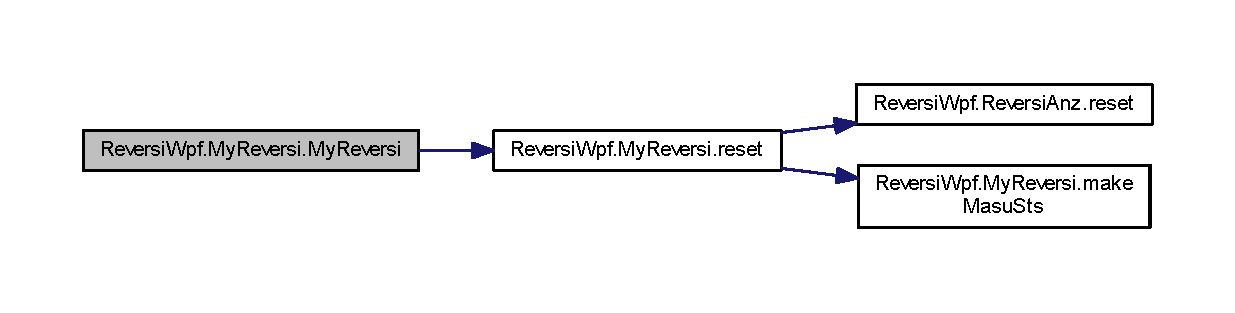
\includegraphics[width=350pt]{class_reversi_wpf_1_1_my_reversi_aff9b8ea39ef41f0d0b84cc5d52af86b2_cgraph}
\end{center}
\end{figure}


\subsection{Member Function Documentation}
\mbox{\Hypertarget{class_reversi_wpf_1_1_my_reversi_a14a3c0720db3ff11196e0c7c34bd80c0}\label{class_reversi_wpf_1_1_my_reversi_a14a3c0720db3ff11196e0c7c34bd80c0}} 
\index{Reversi\+Wpf\+::\+My\+Reversi@{Reversi\+Wpf\+::\+My\+Reversi}!Analysis\+Reversi@{Analysis\+Reversi}}
\index{Analysis\+Reversi@{Analysis\+Reversi}!Reversi\+Wpf\+::\+My\+Reversi@{Reversi\+Wpf\+::\+My\+Reversi}}
\subsubsection{\texorpdfstring{Analysis\+Reversi()}{AnalysisReversi()}}
{\footnotesize\ttfamily void Reversi\+Wpf.\+My\+Reversi.\+Analysis\+Reversi (\begin{DoxyParamCaption}\item[{int}]{b\+Pass\+Ena,  }\item[{int}]{w\+Pass\+Ena }\end{DoxyParamCaption})}



解析を行う 


\begin{DoxyParams}[1]{Parameters}
\mbox{\tt in}  & {\em int} & b\+Pass\+Ena 1=黒パス有効 \\
\hline
\mbox{\tt in}  & {\em int} & w\+Pass\+Ena 1=白パス有効 \\
\hline
\end{DoxyParams}
\begin{DoxyReturn}{Returns}
ありません 
\end{DoxyReturn}
\begin{DoxyAuthor}{Author}
Yuta Yoshinaga 
\end{DoxyAuthor}
\begin{DoxyDate}{Date}
2017.\+10.\+20 
\end{DoxyDate}


Definition at line 948 of file My\+Reversi.\+cs.



Referenced by Reversi\+Wpf.\+Reversi\+Play.\+reset(), Reversi\+Wpf.\+Reversi\+Play.\+reversi\+Play(), and Reversi\+Wpf.\+Reversi\+Play.\+reversi\+Play\+Cpu().

Here is the call graph for this function\+:
\nopagebreak
\begin{figure}[H]
\begin{center}
\leavevmode
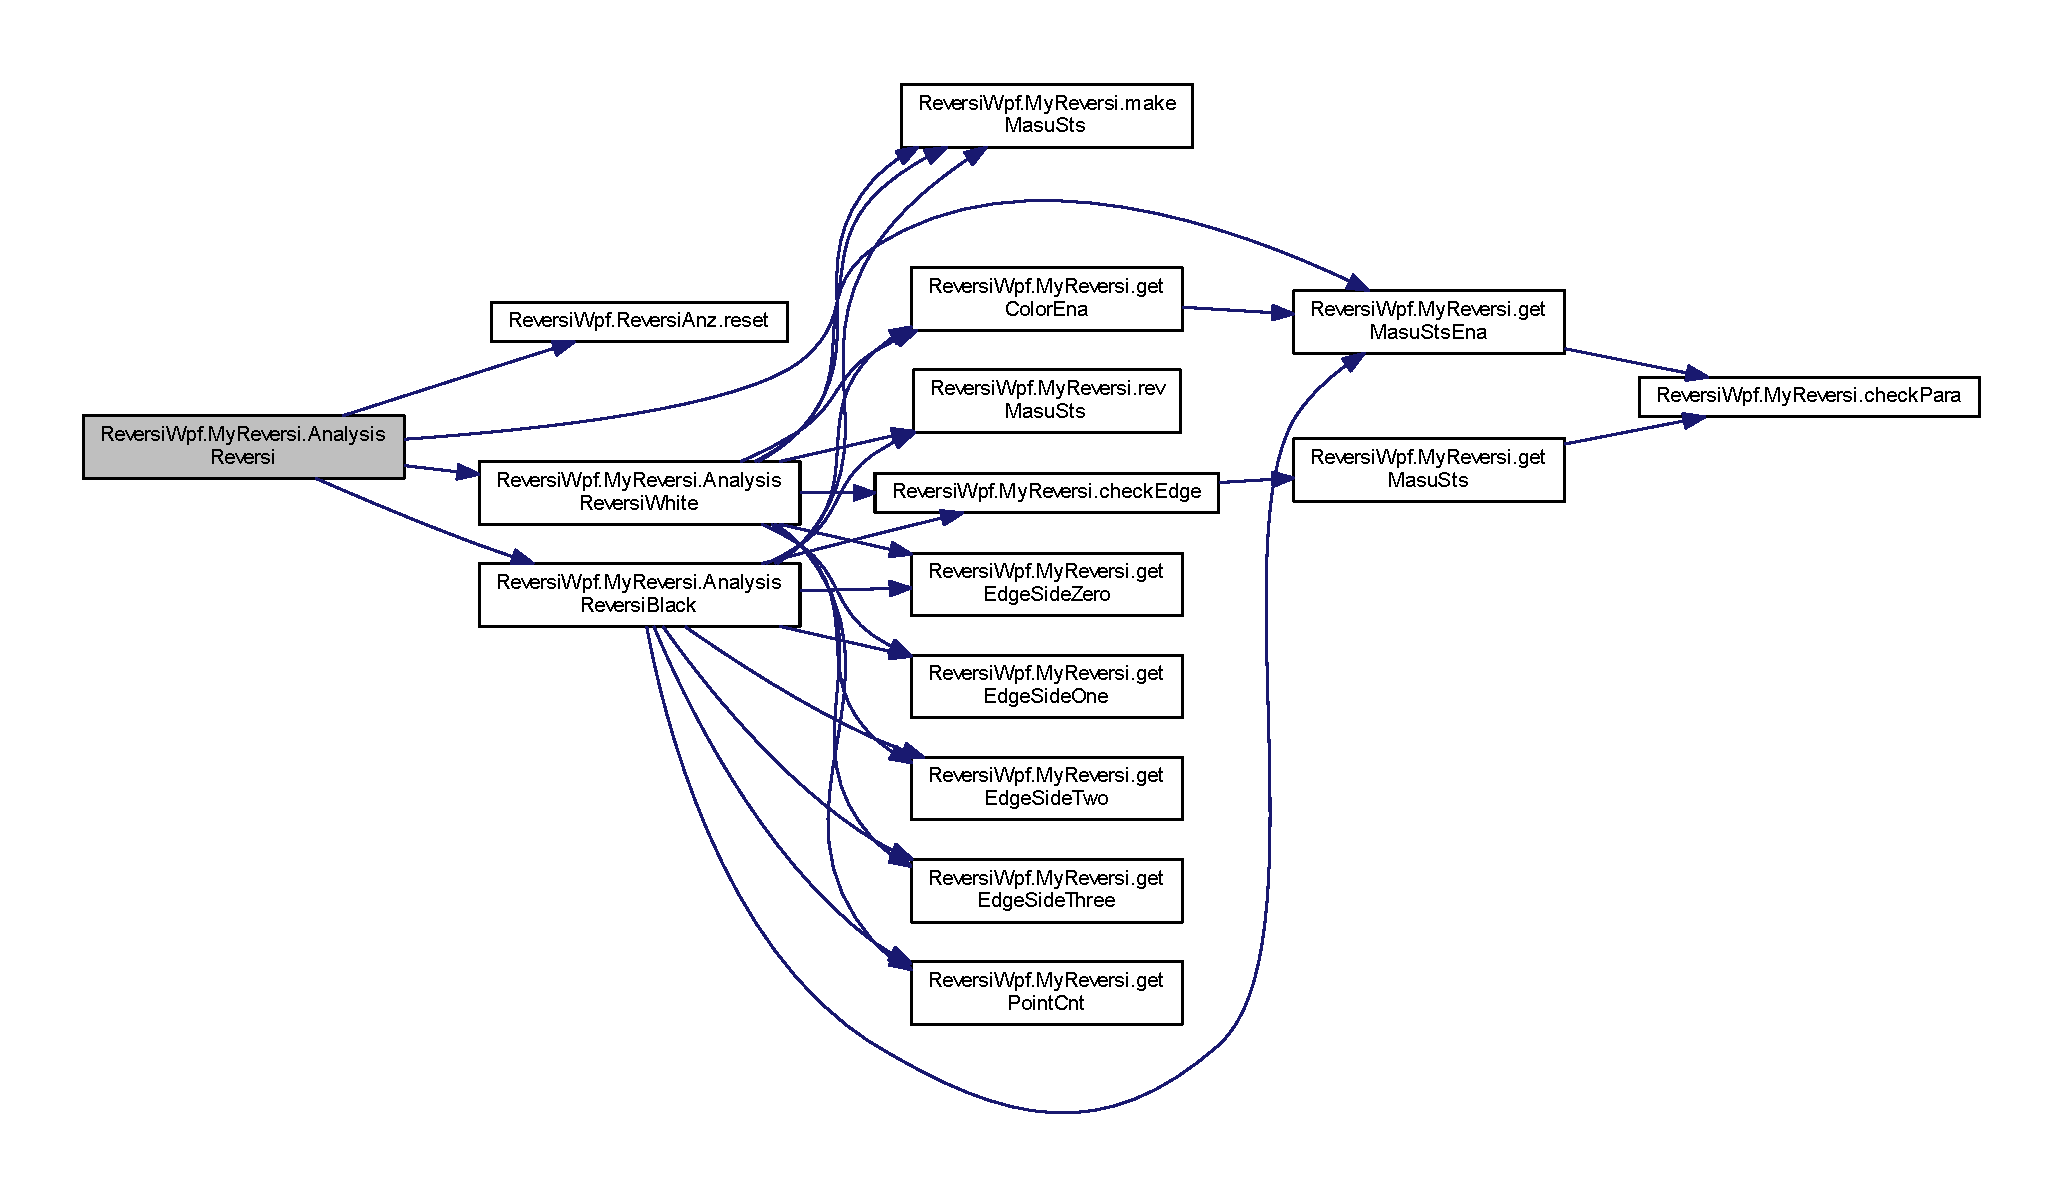
\includegraphics[width=350pt]{class_reversi_wpf_1_1_my_reversi_a14a3c0720db3ff11196e0c7c34bd80c0_cgraph}
\end{center}
\end{figure}
Here is the caller graph for this function\+:
\nopagebreak
\begin{figure}[H]
\begin{center}
\leavevmode
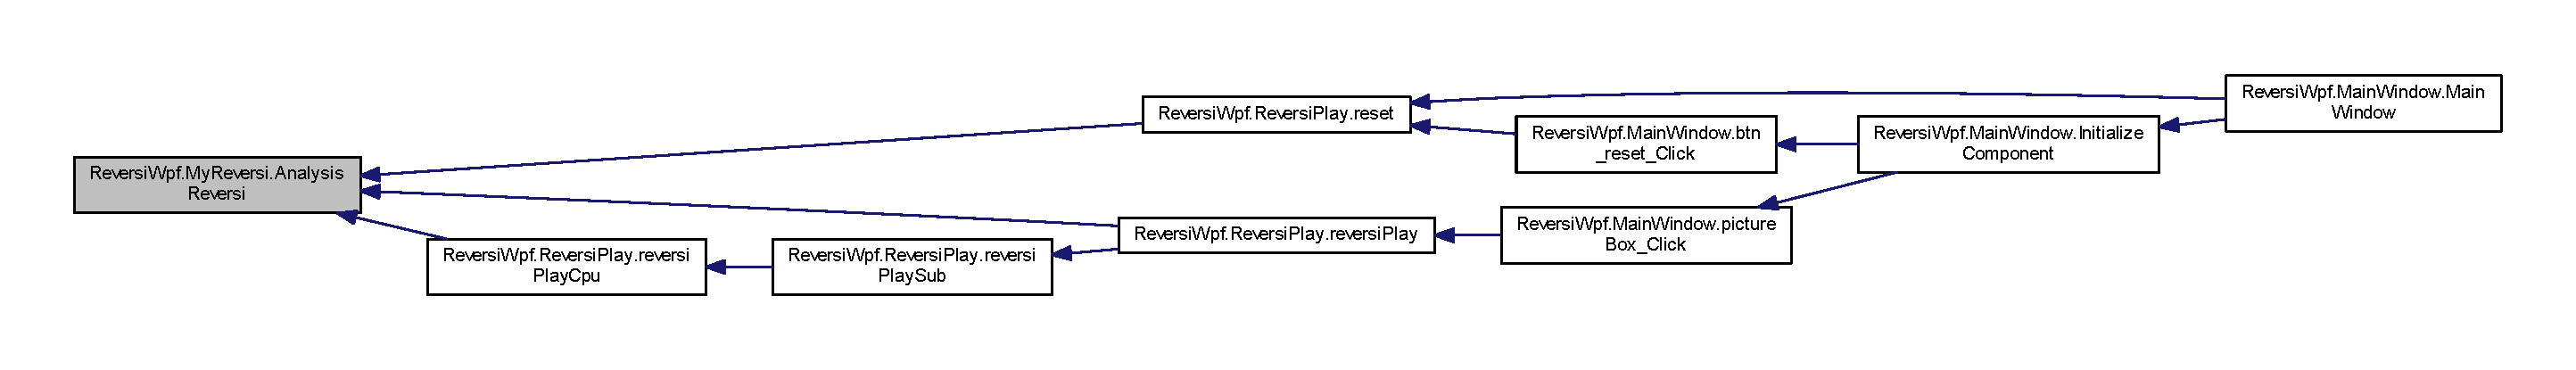
\includegraphics[width=350pt]{class_reversi_wpf_1_1_my_reversi_a14a3c0720db3ff11196e0c7c34bd80c0_icgraph}
\end{center}
\end{figure}
\mbox{\Hypertarget{class_reversi_wpf_1_1_my_reversi_af7ca68ea9f05d79c1debbdc320555098}\label{class_reversi_wpf_1_1_my_reversi_af7ca68ea9f05d79c1debbdc320555098}} 
\index{Reversi\+Wpf\+::\+My\+Reversi@{Reversi\+Wpf\+::\+My\+Reversi}!Analysis\+Reversi\+Black@{Analysis\+Reversi\+Black}}
\index{Analysis\+Reversi\+Black@{Analysis\+Reversi\+Black}!Reversi\+Wpf\+::\+My\+Reversi@{Reversi\+Wpf\+::\+My\+Reversi}}
\subsubsection{\texorpdfstring{Analysis\+Reversi\+Black()}{AnalysisReversiBlack()}}
{\footnotesize\ttfamily void Reversi\+Wpf.\+My\+Reversi.\+Analysis\+Reversi\+Black (\begin{DoxyParamCaption}{ }\end{DoxyParamCaption})\hspace{0.3cm}{\ttfamily [private]}}



解析を行う(黒) 

\begin{DoxyReturn}{Returns}
ありません 
\end{DoxyReturn}
\begin{DoxyAuthor}{Author}
Yuta Yoshinaga 
\end{DoxyAuthor}
\begin{DoxyDate}{Date}
2017.\+10.\+20 
\end{DoxyDate}


Definition at line 670 of file My\+Reversi.\+cs.



Referenced by Reversi\+Wpf.\+My\+Reversi.\+Analysis\+Reversi().

Here is the call graph for this function\+:
\nopagebreak
\begin{figure}[H]
\begin{center}
\leavevmode
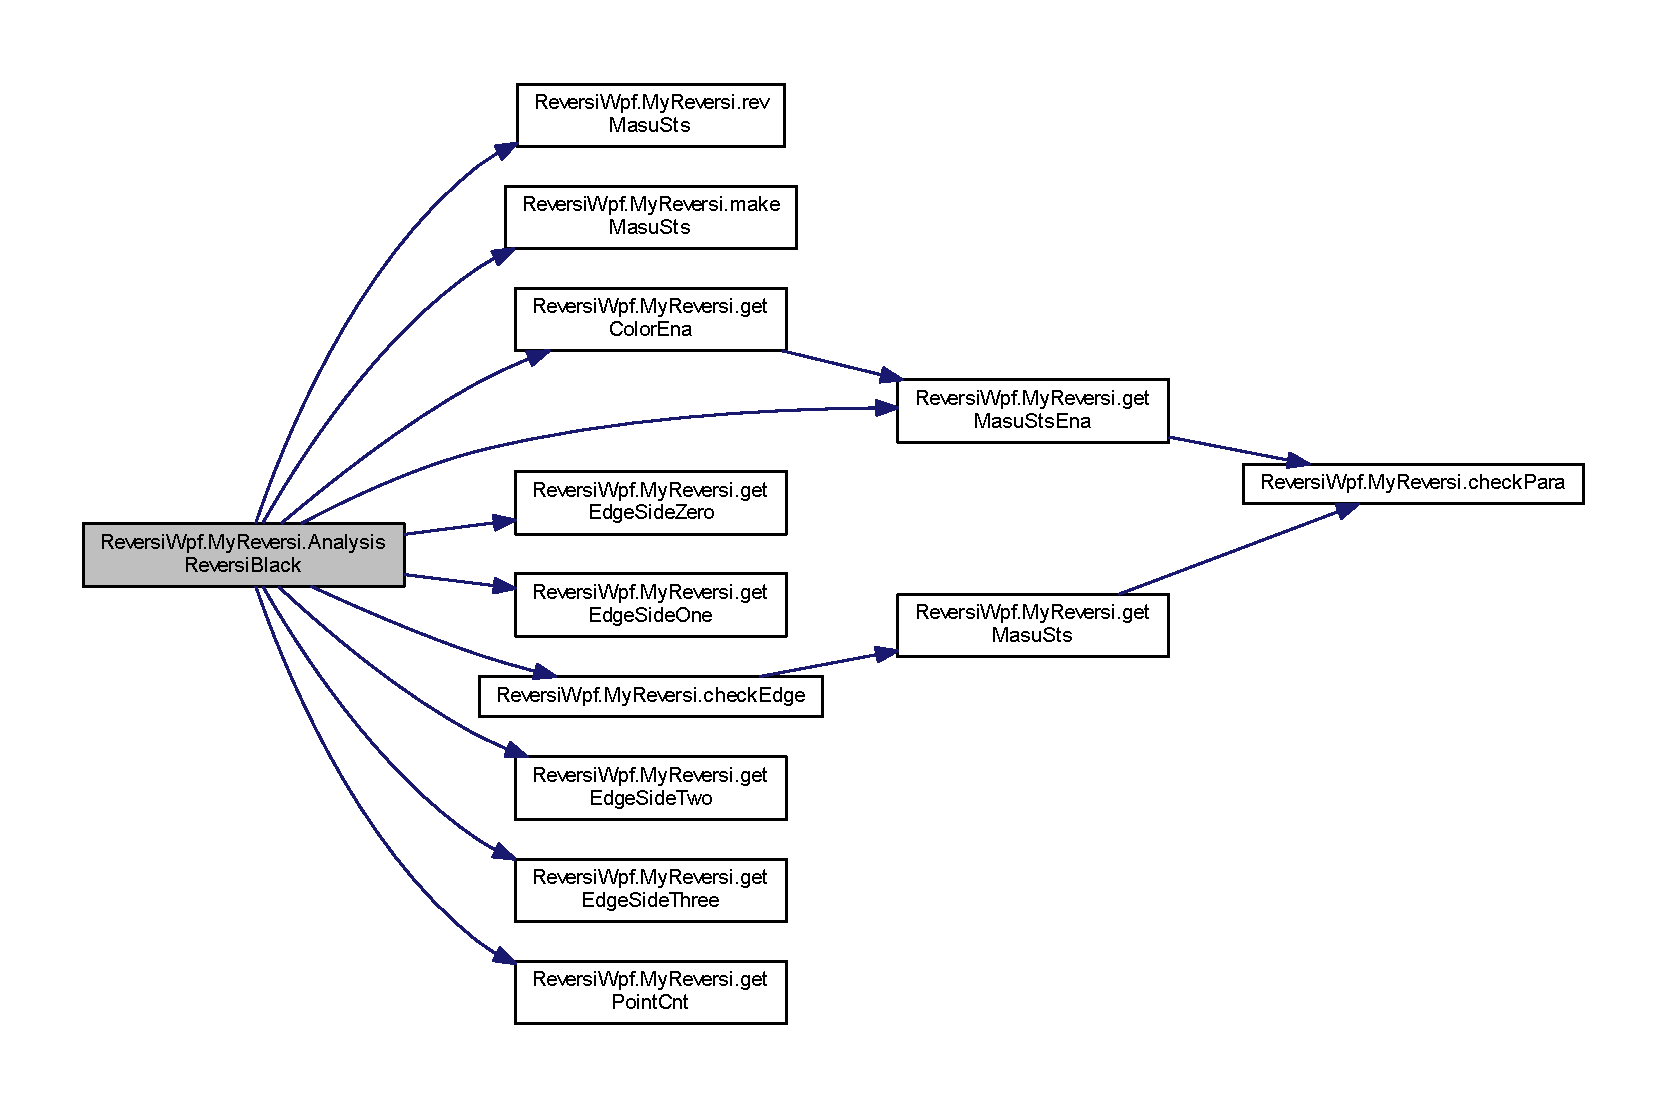
\includegraphics[width=350pt]{class_reversi_wpf_1_1_my_reversi_af7ca68ea9f05d79c1debbdc320555098_cgraph}
\end{center}
\end{figure}
Here is the caller graph for this function\+:
\nopagebreak
\begin{figure}[H]
\begin{center}
\leavevmode
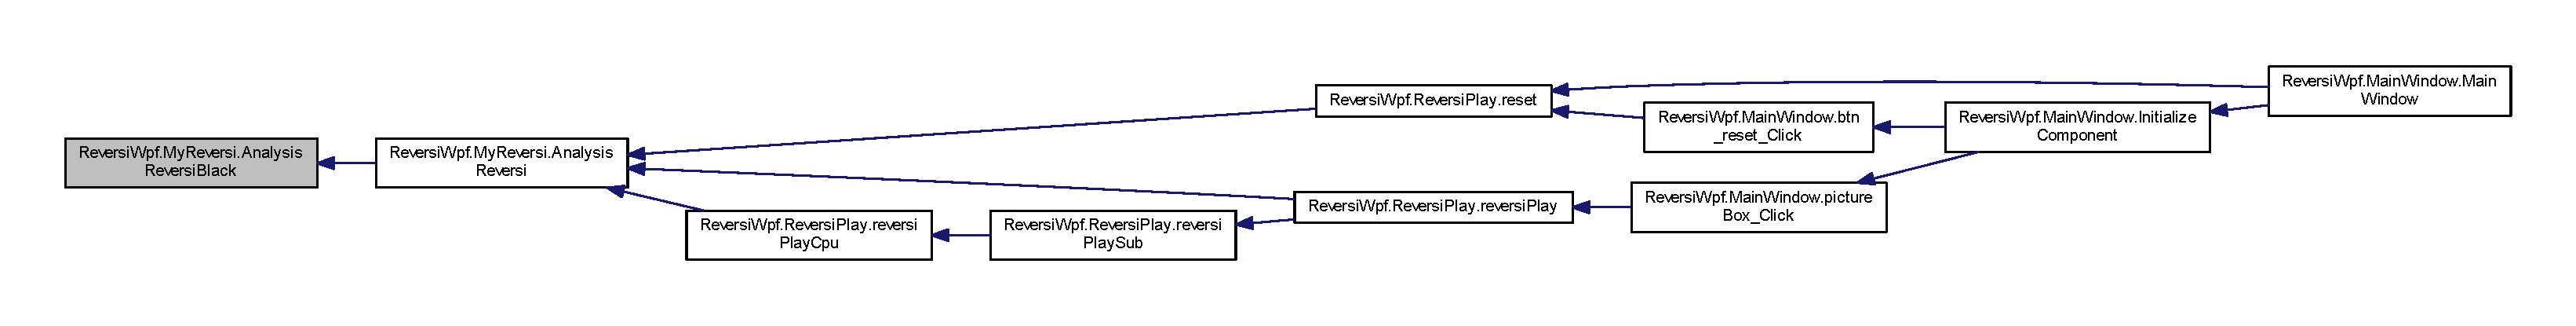
\includegraphics[width=350pt]{class_reversi_wpf_1_1_my_reversi_af7ca68ea9f05d79c1debbdc320555098_icgraph}
\end{center}
\end{figure}
\mbox{\Hypertarget{class_reversi_wpf_1_1_my_reversi_a7be281b0dbae11afb652260b4d30f128}\label{class_reversi_wpf_1_1_my_reversi_a7be281b0dbae11afb652260b4d30f128}} 
\index{Reversi\+Wpf\+::\+My\+Reversi@{Reversi\+Wpf\+::\+My\+Reversi}!Analysis\+Reversi\+White@{Analysis\+Reversi\+White}}
\index{Analysis\+Reversi\+White@{Analysis\+Reversi\+White}!Reversi\+Wpf\+::\+My\+Reversi@{Reversi\+Wpf\+::\+My\+Reversi}}
\subsubsection{\texorpdfstring{Analysis\+Reversi\+White()}{AnalysisReversiWhite()}}
{\footnotesize\ttfamily void Reversi\+Wpf.\+My\+Reversi.\+Analysis\+Reversi\+White (\begin{DoxyParamCaption}{ }\end{DoxyParamCaption})\hspace{0.3cm}{\ttfamily [private]}}



解析を行う(白) 

\begin{DoxyReturn}{Returns}
ありません 
\end{DoxyReturn}
\begin{DoxyAuthor}{Author}
Yuta Yoshinaga 
\end{DoxyAuthor}
\begin{DoxyDate}{Date}
2017.\+10.\+20 
\end{DoxyDate}


Definition at line 808 of file My\+Reversi.\+cs.



Referenced by Reversi\+Wpf.\+My\+Reversi.\+Analysis\+Reversi().

Here is the call graph for this function\+:
\nopagebreak
\begin{figure}[H]
\begin{center}
\leavevmode
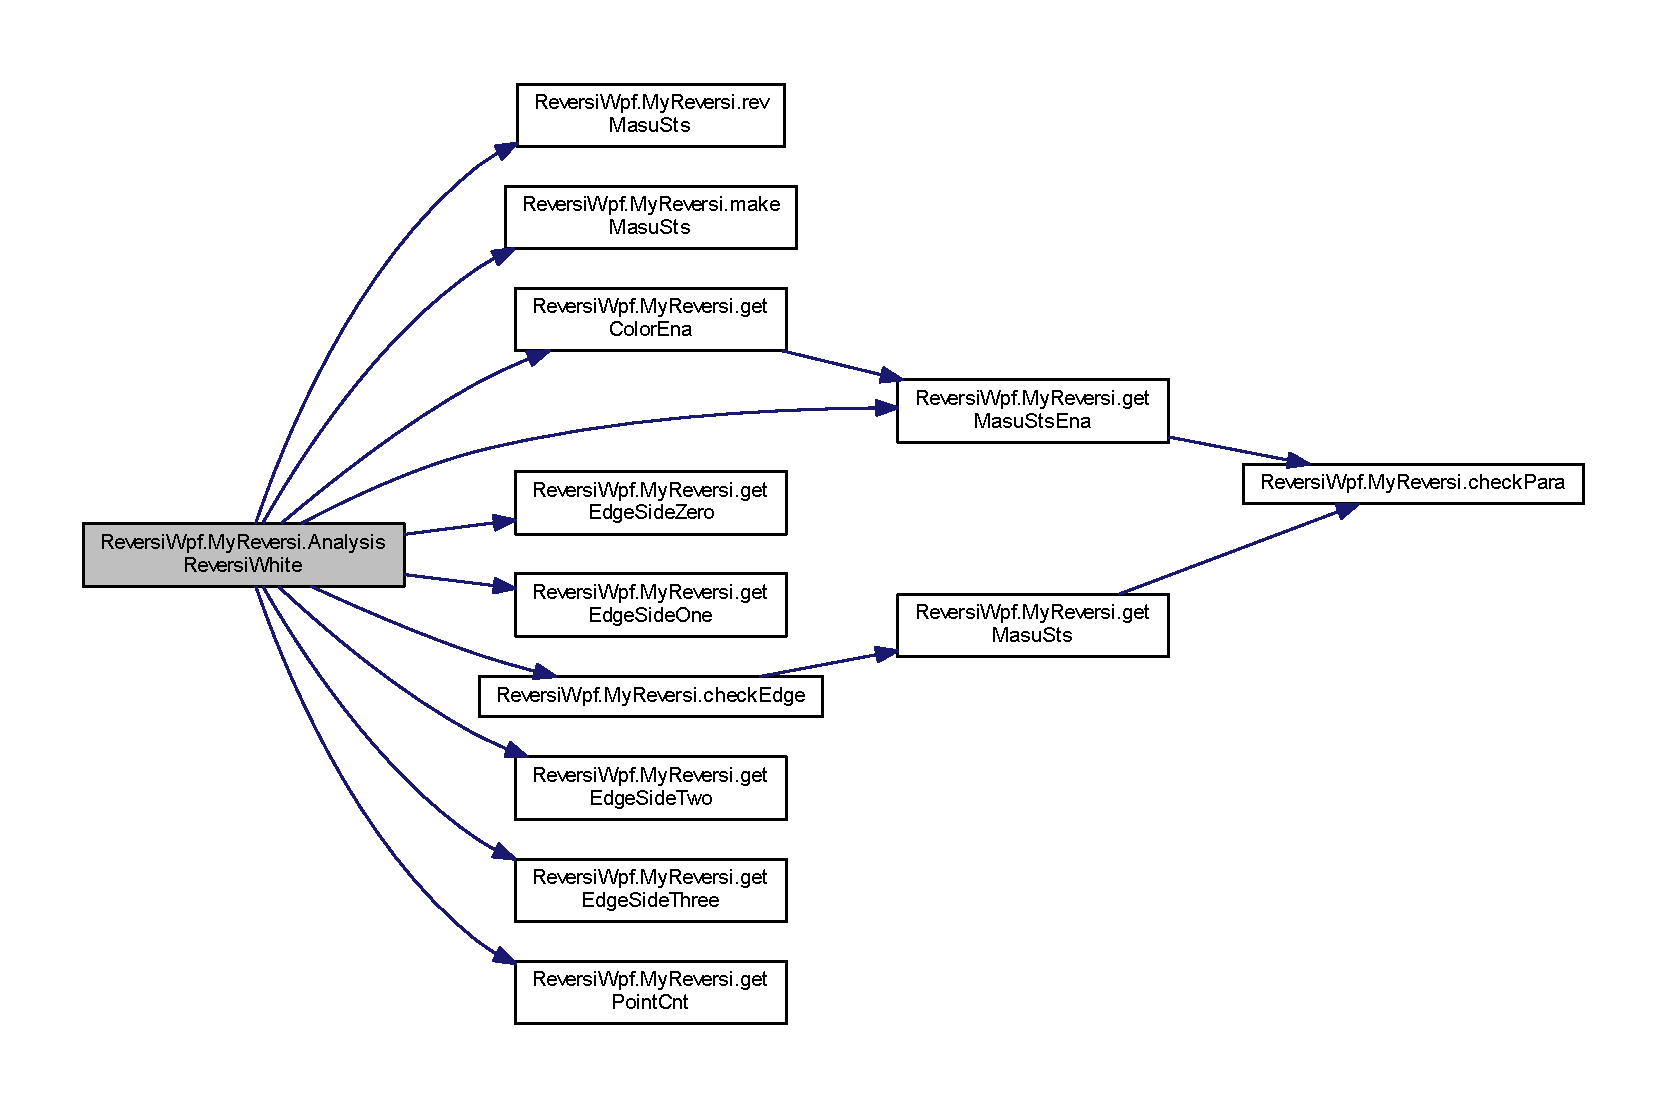
\includegraphics[width=350pt]{class_reversi_wpf_1_1_my_reversi_a7be281b0dbae11afb652260b4d30f128_cgraph}
\end{center}
\end{figure}
Here is the caller graph for this function\+:
\nopagebreak
\begin{figure}[H]
\begin{center}
\leavevmode
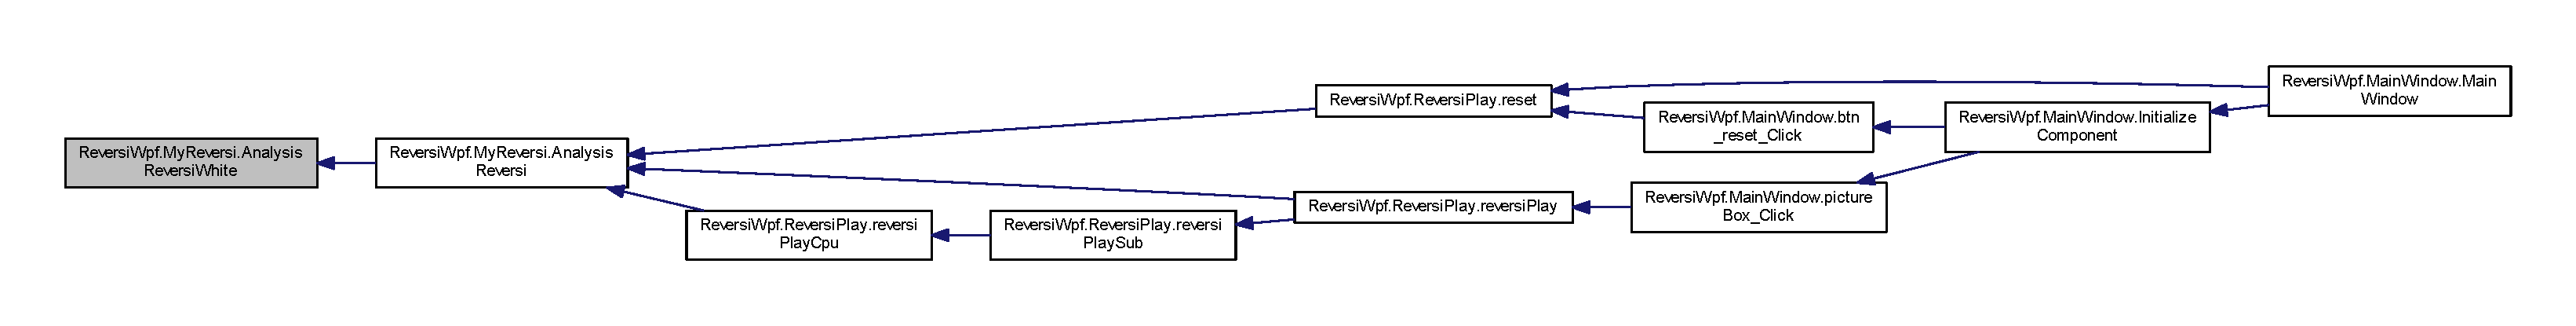
\includegraphics[width=350pt]{class_reversi_wpf_1_1_my_reversi_a7be281b0dbae11afb652260b4d30f128_icgraph}
\end{center}
\end{figure}
\mbox{\Hypertarget{class_reversi_wpf_1_1_my_reversi_acad9426b5389a91f1f42c733b2f2097e}\label{class_reversi_wpf_1_1_my_reversi_acad9426b5389a91f1f42c733b2f2097e}} 
\index{Reversi\+Wpf\+::\+My\+Reversi@{Reversi\+Wpf\+::\+My\+Reversi}!check\+Edge@{check\+Edge}}
\index{check\+Edge@{check\+Edge}!Reversi\+Wpf\+::\+My\+Reversi@{Reversi\+Wpf\+::\+My\+Reversi}}
\subsubsection{\texorpdfstring{check\+Edge()}{checkEdge()}}
{\footnotesize\ttfamily int Reversi\+Wpf.\+My\+Reversi.\+check\+Edge (\begin{DoxyParamCaption}\item[{int}]{color,  }\item[{int}]{y,  }\item[{int}]{x }\end{DoxyParamCaption})}



角の隣に置いても角を取られないマス検索 


\begin{DoxyParams}[1]{Parameters}
\mbox{\tt in}  & {\em int} & color コマ色 \\
\hline
\mbox{\tt in}  & {\em int} & y マスの\+Y座標 \\
\hline
\mbox{\tt in}  & {\em int} & x マスの\+X座標 \\
\hline
\end{DoxyParams}
\begin{DoxyReturn}{Returns}
0 \+: 取られる それ以外 \+: 取られない 
\end{DoxyReturn}
\begin{DoxyAuthor}{Author}
Yuta Yoshinaga 
\end{DoxyAuthor}
\begin{DoxyDate}{Date}
2017.\+10.\+20 
\end{DoxyDate}


Definition at line 1312 of file My\+Reversi.\+cs.



Referenced by Reversi\+Wpf.\+My\+Reversi.\+Analysis\+Reversi\+Black(), Reversi\+Wpf.\+My\+Reversi.\+Analysis\+Reversi\+White(), and Reversi\+Wpf.\+Reversi\+Play.\+reversi\+Play\+Cpu().

Here is the call graph for this function\+:
\nopagebreak
\begin{figure}[H]
\begin{center}
\leavevmode
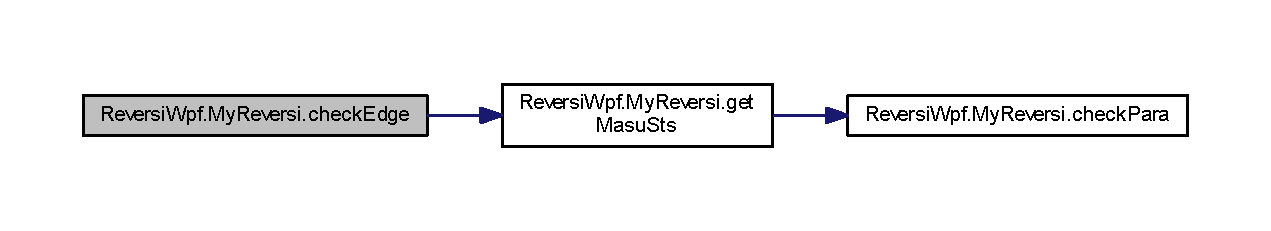
\includegraphics[width=350pt]{class_reversi_wpf_1_1_my_reversi_acad9426b5389a91f1f42c733b2f2097e_cgraph}
\end{center}
\end{figure}
Here is the caller graph for this function\+:
\nopagebreak
\begin{figure}[H]
\begin{center}
\leavevmode
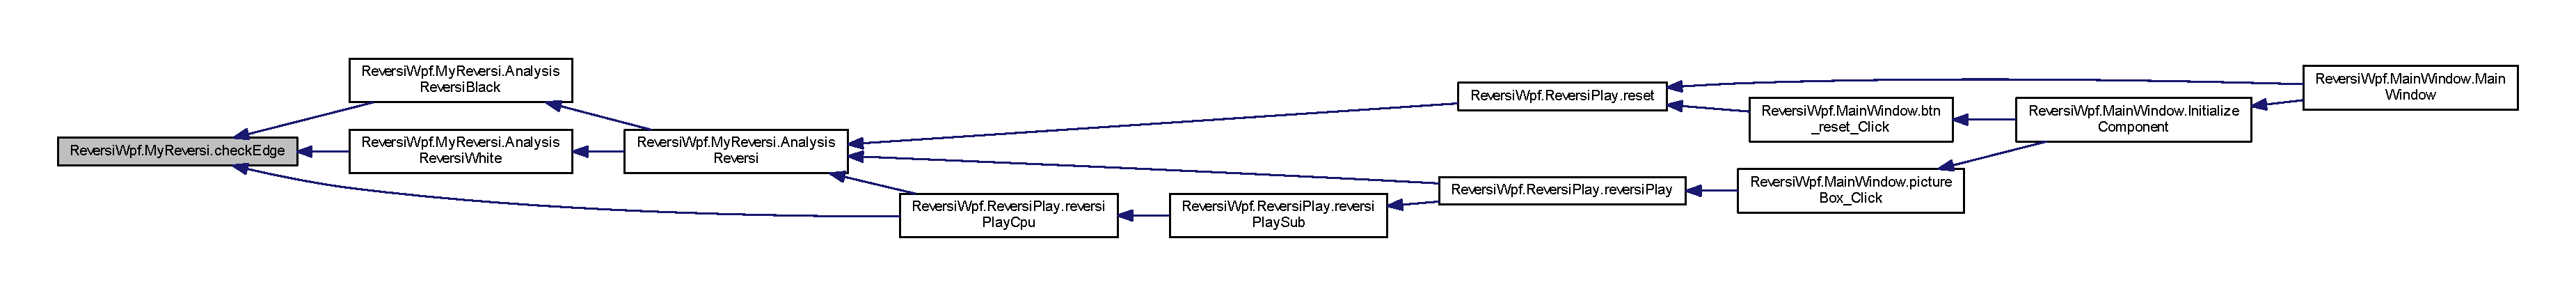
\includegraphics[width=350pt]{class_reversi_wpf_1_1_my_reversi_acad9426b5389a91f1f42c733b2f2097e_icgraph}
\end{center}
\end{figure}
\mbox{\Hypertarget{class_reversi_wpf_1_1_my_reversi_adc98d24744c8e50f62f94b9441f582c5}\label{class_reversi_wpf_1_1_my_reversi_adc98d24744c8e50f62f94b9441f582c5}} 
\index{Reversi\+Wpf\+::\+My\+Reversi@{Reversi\+Wpf\+::\+My\+Reversi}!check\+Para@{check\+Para}}
\index{check\+Para@{check\+Para}!Reversi\+Wpf\+::\+My\+Reversi@{Reversi\+Wpf\+::\+My\+Reversi}}
\subsubsection{\texorpdfstring{check\+Para()}{checkPara()}}
{\footnotesize\ttfamily int Reversi\+Wpf.\+My\+Reversi.\+check\+Para (\begin{DoxyParamCaption}\item[{int}]{para,  }\item[{int}]{min,  }\item[{int}]{max }\end{DoxyParamCaption})\hspace{0.3cm}{\ttfamily [private]}}



パラメーター範囲チェック 


\begin{DoxyParams}[1]{Parameters}
\mbox{\tt in}  & {\em int} & para チェックパラメーター \\
\hline
\mbox{\tt in}  & {\em int} & min パラメーター最小値 \\
\hline
\mbox{\tt in}  & {\em int} & max パラメーター最大値 \\
\hline
\end{DoxyParams}
\begin{DoxyReturn}{Returns}
0 \+: 成功 それ以外 \+: 失敗 
\end{DoxyReturn}
\begin{DoxyAuthor}{Author}
Yuta Yoshinaga 
\end{DoxyAuthor}
\begin{DoxyDate}{Date}
2017.\+10.\+20 
\end{DoxyDate}


Definition at line 655 of file My\+Reversi.\+cs.



Referenced by Reversi\+Wpf.\+My\+Reversi.\+get\+History(), Reversi\+Wpf.\+My\+Reversi.\+get\+Masu\+Sts(), Reversi\+Wpf.\+My\+Reversi.\+get\+Masu\+Sts\+Cnt(), Reversi\+Wpf.\+My\+Reversi.\+get\+Masu\+Sts\+Ena(), Reversi\+Wpf.\+My\+Reversi.\+get\+Masu\+Sts\+Old(), Reversi\+Wpf.\+My\+Reversi.\+get\+Pass\+Ena(), Reversi\+Wpf.\+My\+Reversi.\+get\+Point(), Reversi\+Wpf.\+My\+Reversi.\+get\+Point\+Anz(), and Reversi\+Wpf.\+My\+Reversi.\+set\+Masu\+Cnt().

Here is the caller graph for this function\+:
\nopagebreak
\begin{figure}[H]
\begin{center}
\leavevmode
\includegraphics[width=350pt]{class_reversi_wpf_1_1_my_reversi_adc98d24744c8e50f62f94b9441f582c5_icgraph}
\end{center}
\end{figure}
\mbox{\Hypertarget{class_reversi_wpf_1_1_my_reversi_aff9b97e9e4102966ea558428255974e2}\label{class_reversi_wpf_1_1_my_reversi_aff9b97e9e4102966ea558428255974e2}} 
\index{Reversi\+Wpf\+::\+My\+Reversi@{Reversi\+Wpf\+::\+My\+Reversi}!Clone@{Clone}}
\index{Clone@{Clone}!Reversi\+Wpf\+::\+My\+Reversi@{Reversi\+Wpf\+::\+My\+Reversi}}
\subsubsection{\texorpdfstring{Clone()}{Clone()}}
{\footnotesize\ttfamily \hyperlink{class_reversi_wpf_1_1_my_reversi}{My\+Reversi} Reversi\+Wpf.\+My\+Reversi.\+Clone (\begin{DoxyParamCaption}{ }\end{DoxyParamCaption})}



コピー 

\begin{DoxyReturn}{Returns}
オブジェクトコピー 
\end{DoxyReturn}
\begin{DoxyAuthor}{Author}
Yuta Yoshinaga 
\end{DoxyAuthor}
\begin{DoxyDate}{Date}
2017.\+10.\+20 
\end{DoxyDate}


Definition at line 230 of file My\+Reversi.\+cs.

\mbox{\Hypertarget{class_reversi_wpf_1_1_my_reversi_a57482d7118dad2c5d104e186acd5212b}\label{class_reversi_wpf_1_1_my_reversi_a57482d7118dad2c5d104e186acd5212b}} 
\index{Reversi\+Wpf\+::\+My\+Reversi@{Reversi\+Wpf\+::\+My\+Reversi}!get\+Bet\+Cnt@{get\+Bet\+Cnt}}
\index{get\+Bet\+Cnt@{get\+Bet\+Cnt}!Reversi\+Wpf\+::\+My\+Reversi@{Reversi\+Wpf\+::\+My\+Reversi}}
\subsubsection{\texorpdfstring{get\+Bet\+Cnt()}{getBetCnt()}}
{\footnotesize\ttfamily int Reversi\+Wpf.\+My\+Reversi.\+get\+Bet\+Cnt (\begin{DoxyParamCaption}\item[{int}]{color }\end{DoxyParamCaption})}



コマ数取得 


\begin{DoxyParams}[1]{Parameters}
\mbox{\tt in}  & {\em int} & color コマ色 \\
\hline
\end{DoxyParams}
\begin{DoxyReturn}{Returns}
コマ数取得 
\end{DoxyReturn}
\begin{DoxyAuthor}{Author}
Yuta Yoshinaga 
\end{DoxyAuthor}
\begin{DoxyDate}{Date}
2017.\+10.\+20 
\end{DoxyDate}


Definition at line 1215 of file My\+Reversi.\+cs.



Referenced by Reversi\+Wpf.\+Reversi\+Play.\+exec\+Message(), Reversi\+Wpf.\+Reversi\+Play.\+game\+End\+Anim\+Exec(), Reversi\+Wpf.\+Reversi\+Play.\+reversi\+Play\+Cpu(), and Reversi\+Wpf.\+Reversi\+Play.\+reversi\+Play\+End().

Here is the caller graph for this function\+:
\nopagebreak
\begin{figure}[H]
\begin{center}
\leavevmode
\includegraphics[width=350pt]{class_reversi_wpf_1_1_my_reversi_a57482d7118dad2c5d104e186acd5212b_icgraph}
\end{center}
\end{figure}
\mbox{\Hypertarget{class_reversi_wpf_1_1_my_reversi_a9a7c386e4b5007a937865ab301774c9e}\label{class_reversi_wpf_1_1_my_reversi_a9a7c386e4b5007a937865ab301774c9e}} 
\index{Reversi\+Wpf\+::\+My\+Reversi@{Reversi\+Wpf\+::\+My\+Reversi}!get\+Color\+Ena@{get\+Color\+Ena}}
\index{get\+Color\+Ena@{get\+Color\+Ena}!Reversi\+Wpf\+::\+My\+Reversi@{Reversi\+Wpf\+::\+My\+Reversi}}
\subsubsection{\texorpdfstring{get\+Color\+Ena()}{getColorEna()}}
{\footnotesize\ttfamily int Reversi\+Wpf.\+My\+Reversi.\+get\+Color\+Ena (\begin{DoxyParamCaption}\item[{int}]{color }\end{DoxyParamCaption})}



指定色が現在置ける場所があるかチェック 


\begin{DoxyParams}[1]{Parameters}
\mbox{\tt in}  & {\em int} & color コマ色 \\
\hline
\end{DoxyParams}
\begin{DoxyReturn}{Returns}
0 \+: 成功 それ以外 \+: 失敗 
\end{DoxyReturn}
\begin{DoxyAuthor}{Author}
Yuta Yoshinaga 
\end{DoxyAuthor}
\begin{DoxyDate}{Date}
2017.\+10.\+20 
\end{DoxyDate}


Definition at line 1063 of file My\+Reversi.\+cs.



Referenced by Reversi\+Wpf.\+My\+Reversi.\+Analysis\+Reversi\+Black(), Reversi\+Wpf.\+My\+Reversi.\+Analysis\+Reversi\+White(), Reversi\+Wpf.\+My\+Reversi.\+get\+Game\+End\+Sts(), Reversi\+Wpf.\+Reversi\+Play.\+reversi\+Play(), and Reversi\+Wpf.\+Reversi\+Play.\+reversi\+Play\+Sub().

Here is the call graph for this function\+:
\nopagebreak
\begin{figure}[H]
\begin{center}
\leavevmode
\includegraphics[width=350pt]{class_reversi_wpf_1_1_my_reversi_a9a7c386e4b5007a937865ab301774c9e_cgraph}
\end{center}
\end{figure}
Here is the caller graph for this function\+:
\nopagebreak
\begin{figure}[H]
\begin{center}
\leavevmode
\includegraphics[width=350pt]{class_reversi_wpf_1_1_my_reversi_a9a7c386e4b5007a937865ab301774c9e_icgraph}
\end{center}
\end{figure}
\mbox{\Hypertarget{class_reversi_wpf_1_1_my_reversi_a6e9641216f52b0c384f43a26cfea981f}\label{class_reversi_wpf_1_1_my_reversi_a6e9641216f52b0c384f43a26cfea981f}} 
\index{Reversi\+Wpf\+::\+My\+Reversi@{Reversi\+Wpf\+::\+My\+Reversi}!get\+Edge\+Side\+One@{get\+Edge\+Side\+One}}
\index{get\+Edge\+Side\+One@{get\+Edge\+Side\+One}!Reversi\+Wpf\+::\+My\+Reversi@{Reversi\+Wpf\+::\+My\+Reversi}}
\subsubsection{\texorpdfstring{get\+Edge\+Side\+One()}{getEdgeSideOne()}}
{\footnotesize\ttfamily int Reversi\+Wpf.\+My\+Reversi.\+get\+Edge\+Side\+One (\begin{DoxyParamCaption}\item[{int}]{y,  }\item[{int}]{x }\end{DoxyParamCaption})}



指定座標が角の一つ手前か取得 


\begin{DoxyParams}[1]{Parameters}
\mbox{\tt in}  & {\em int} & y Y座標 \\
\hline
\mbox{\tt in}  & {\em int} & x X座標 \\
\hline
\end{DoxyParams}
\begin{DoxyReturn}{Returns}
0 \+: 成功 それ以外 \+: 失敗 
\end{DoxyReturn}
\begin{DoxyAuthor}{Author}
Yuta Yoshinaga 
\end{DoxyAuthor}
\begin{DoxyDate}{Date}
2017.\+10.\+20 
\end{DoxyDate}


Definition at line 1454 of file My\+Reversi.\+cs.



Referenced by Reversi\+Wpf.\+My\+Reversi.\+Analysis\+Reversi\+Black(), Reversi\+Wpf.\+My\+Reversi.\+Analysis\+Reversi\+White(), and Reversi\+Wpf.\+Reversi\+Play.\+reversi\+Play\+Cpu().

Here is the caller graph for this function\+:
\nopagebreak
\begin{figure}[H]
\begin{center}
\leavevmode
\includegraphics[width=350pt]{class_reversi_wpf_1_1_my_reversi_a6e9641216f52b0c384f43a26cfea981f_icgraph}
\end{center}
\end{figure}
\mbox{\Hypertarget{class_reversi_wpf_1_1_my_reversi_a278da279bc20775b0849a1316729d6a3}\label{class_reversi_wpf_1_1_my_reversi_a278da279bc20775b0849a1316729d6a3}} 
\index{Reversi\+Wpf\+::\+My\+Reversi@{Reversi\+Wpf\+::\+My\+Reversi}!get\+Edge\+Side\+Three@{get\+Edge\+Side\+Three}}
\index{get\+Edge\+Side\+Three@{get\+Edge\+Side\+Three}!Reversi\+Wpf\+::\+My\+Reversi@{Reversi\+Wpf\+::\+My\+Reversi}}
\subsubsection{\texorpdfstring{get\+Edge\+Side\+Three()}{getEdgeSideThree()}}
{\footnotesize\ttfamily int Reversi\+Wpf.\+My\+Reversi.\+get\+Edge\+Side\+Three (\begin{DoxyParamCaption}\item[{int}]{y,  }\item[{int}]{x }\end{DoxyParamCaption})}



指定座標が角の三つ以上手前か取得 


\begin{DoxyParams}[1]{Parameters}
\mbox{\tt in}  & {\em int} & y Y座標 \\
\hline
\mbox{\tt in}  & {\em int} & x X座標 \\
\hline
\end{DoxyParams}
\begin{DoxyReturn}{Returns}
0 \+: 成功 それ以外 \+: 失敗 
\end{DoxyReturn}
\begin{DoxyAuthor}{Author}
Yuta Yoshinaga 
\end{DoxyAuthor}
\begin{DoxyDate}{Date}
2017.\+10.\+20 
\end{DoxyDate}


Definition at line 1518 of file My\+Reversi.\+cs.



Referenced by Reversi\+Wpf.\+My\+Reversi.\+Analysis\+Reversi\+Black(), Reversi\+Wpf.\+My\+Reversi.\+Analysis\+Reversi\+White(), and Reversi\+Wpf.\+Reversi\+Play.\+reversi\+Play\+Cpu().

Here is the caller graph for this function\+:
\nopagebreak
\begin{figure}[H]
\begin{center}
\leavevmode
\includegraphics[width=350pt]{class_reversi_wpf_1_1_my_reversi_a278da279bc20775b0849a1316729d6a3_icgraph}
\end{center}
\end{figure}
\mbox{\Hypertarget{class_reversi_wpf_1_1_my_reversi_ae59ceaeded22519213df314ab31b45d1}\label{class_reversi_wpf_1_1_my_reversi_ae59ceaeded22519213df314ab31b45d1}} 
\index{Reversi\+Wpf\+::\+My\+Reversi@{Reversi\+Wpf\+::\+My\+Reversi}!get\+Edge\+Side\+Two@{get\+Edge\+Side\+Two}}
\index{get\+Edge\+Side\+Two@{get\+Edge\+Side\+Two}!Reversi\+Wpf\+::\+My\+Reversi@{Reversi\+Wpf\+::\+My\+Reversi}}
\subsubsection{\texorpdfstring{get\+Edge\+Side\+Two()}{getEdgeSideTwo()}}
{\footnotesize\ttfamily int Reversi\+Wpf.\+My\+Reversi.\+get\+Edge\+Side\+Two (\begin{DoxyParamCaption}\item[{int}]{y,  }\item[{int}]{x }\end{DoxyParamCaption})}



指定座標が角の二つ手前か取得 


\begin{DoxyParams}[1]{Parameters}
\mbox{\tt in}  & {\em int} & y Y座標 \\
\hline
\mbox{\tt in}  & {\em int} & x X座標 \\
\hline
\end{DoxyParams}
\begin{DoxyReturn}{Returns}
0 \+: 成功 それ以外 \+: 失敗 
\end{DoxyReturn}
\begin{DoxyAuthor}{Author}
Yuta Yoshinaga 
\end{DoxyAuthor}
\begin{DoxyDate}{Date}
2017.\+10.\+20 
\end{DoxyDate}


Definition at line 1486 of file My\+Reversi.\+cs.



Referenced by Reversi\+Wpf.\+My\+Reversi.\+Analysis\+Reversi\+Black(), Reversi\+Wpf.\+My\+Reversi.\+Analysis\+Reversi\+White(), and Reversi\+Wpf.\+Reversi\+Play.\+reversi\+Play\+Cpu().

Here is the caller graph for this function\+:
\nopagebreak
\begin{figure}[H]
\begin{center}
\leavevmode
\includegraphics[width=350pt]{class_reversi_wpf_1_1_my_reversi_ae59ceaeded22519213df314ab31b45d1_icgraph}
\end{center}
\end{figure}
\mbox{\Hypertarget{class_reversi_wpf_1_1_my_reversi_a3418fce34fd194987dc0efcd7aa654a4}\label{class_reversi_wpf_1_1_my_reversi_a3418fce34fd194987dc0efcd7aa654a4}} 
\index{Reversi\+Wpf\+::\+My\+Reversi@{Reversi\+Wpf\+::\+My\+Reversi}!get\+Edge\+Side\+Zero@{get\+Edge\+Side\+Zero}}
\index{get\+Edge\+Side\+Zero@{get\+Edge\+Side\+Zero}!Reversi\+Wpf\+::\+My\+Reversi@{Reversi\+Wpf\+::\+My\+Reversi}}
\subsubsection{\texorpdfstring{get\+Edge\+Side\+Zero()}{getEdgeSideZero()}}
{\footnotesize\ttfamily int Reversi\+Wpf.\+My\+Reversi.\+get\+Edge\+Side\+Zero (\begin{DoxyParamCaption}\item[{int}]{y,  }\item[{int}]{x }\end{DoxyParamCaption})}



指定座標が角か取得 


\begin{DoxyParams}[1]{Parameters}
\mbox{\tt in}  & {\em int} & y Y座標 \\
\hline
\mbox{\tt in}  & {\em int} & x X座標 \\
\hline
\end{DoxyParams}
\begin{DoxyReturn}{Returns}
0 \+: 成功 それ以外 \+: 失敗 
\end{DoxyReturn}
\begin{DoxyAuthor}{Author}
Yuta Yoshinaga 
\end{DoxyAuthor}
\begin{DoxyDate}{Date}
2017.\+10.\+20 
\end{DoxyDate}


Definition at line 1430 of file My\+Reversi.\+cs.



Referenced by Reversi\+Wpf.\+My\+Reversi.\+Analysis\+Reversi\+Black(), Reversi\+Wpf.\+My\+Reversi.\+Analysis\+Reversi\+White(), and Reversi\+Wpf.\+Reversi\+Play.\+reversi\+Play\+Cpu().

Here is the caller graph for this function\+:
\nopagebreak
\begin{figure}[H]
\begin{center}
\leavevmode
\includegraphics[width=350pt]{class_reversi_wpf_1_1_my_reversi_a3418fce34fd194987dc0efcd7aa654a4_icgraph}
\end{center}
\end{figure}
\mbox{\Hypertarget{class_reversi_wpf_1_1_my_reversi_a77a81c9c08a6dadcab0dd5741de1b88b}\label{class_reversi_wpf_1_1_my_reversi_a77a81c9c08a6dadcab0dd5741de1b88b}} 
\index{Reversi\+Wpf\+::\+My\+Reversi@{Reversi\+Wpf\+::\+My\+Reversi}!get\+Game\+End\+Sts@{get\+Game\+End\+Sts}}
\index{get\+Game\+End\+Sts@{get\+Game\+End\+Sts}!Reversi\+Wpf\+::\+My\+Reversi@{Reversi\+Wpf\+::\+My\+Reversi}}
\subsubsection{\texorpdfstring{get\+Game\+End\+Sts()}{getGameEndSts()}}
{\footnotesize\ttfamily int Reversi\+Wpf.\+My\+Reversi.\+get\+Game\+End\+Sts (\begin{DoxyParamCaption}{ }\end{DoxyParamCaption})}



ゲーム終了かチェック 

\begin{DoxyReturn}{Returns}
0 \+: 続行 それ以外 \+: ゲーム終了 
\end{DoxyReturn}
\begin{DoxyAuthor}{Author}
Yuta Yoshinaga 
\end{DoxyAuthor}
\begin{DoxyDate}{Date}
2017.\+10.\+20 
\end{DoxyDate}


Definition at line 1085 of file My\+Reversi.\+cs.



Referenced by Reversi\+Wpf.\+Reversi\+Play.\+reversi\+Play(), and Reversi\+Wpf.\+Reversi\+Play.\+reversi\+Play\+Sub().

Here is the call graph for this function\+:
\nopagebreak
\begin{figure}[H]
\begin{center}
\leavevmode
\includegraphics[width=350pt]{class_reversi_wpf_1_1_my_reversi_a77a81c9c08a6dadcab0dd5741de1b88b_cgraph}
\end{center}
\end{figure}
Here is the caller graph for this function\+:
\nopagebreak
\begin{figure}[H]
\begin{center}
\leavevmode
\includegraphics[width=350pt]{class_reversi_wpf_1_1_my_reversi_a77a81c9c08a6dadcab0dd5741de1b88b_icgraph}
\end{center}
\end{figure}
\mbox{\Hypertarget{class_reversi_wpf_1_1_my_reversi_aa85fcb151ab7c188b0637b9eb9269baa}\label{class_reversi_wpf_1_1_my_reversi_aa85fcb151ab7c188b0637b9eb9269baa}} 
\index{Reversi\+Wpf\+::\+My\+Reversi@{Reversi\+Wpf\+::\+My\+Reversi}!get\+History@{get\+History}}
\index{get\+History@{get\+History}!Reversi\+Wpf\+::\+My\+Reversi@{Reversi\+Wpf\+::\+My\+Reversi}}
\subsubsection{\texorpdfstring{get\+History()}{getHistory()}}
{\footnotesize\ttfamily \hyperlink{class_reversi_wpf_1_1_reversi_history}{Reversi\+History} Reversi\+Wpf.\+My\+Reversi.\+get\+History (\begin{DoxyParamCaption}\item[{int}]{num }\end{DoxyParamCaption})}



履歴取得 


\begin{DoxyParams}[1]{Parameters}
\mbox{\tt in}  & {\em int} & num ポイント \\
\hline
\end{DoxyParams}
\begin{DoxyReturn}{Returns}
履歴 null \+: 失敗 
\end{DoxyReturn}
\begin{DoxyAuthor}{Author}
Yuta Yoshinaga 
\end{DoxyAuthor}
\begin{DoxyDate}{Date}
2017.\+10.\+20 
\end{DoxyDate}


Definition at line 1256 of file My\+Reversi.\+cs.

Here is the call graph for this function\+:
\nopagebreak
\begin{figure}[H]
\begin{center}
\leavevmode
\includegraphics[width=350pt]{class_reversi_wpf_1_1_my_reversi_aa85fcb151ab7c188b0637b9eb9269baa_cgraph}
\end{center}
\end{figure}
\mbox{\Hypertarget{class_reversi_wpf_1_1_my_reversi_a9e6ba44101405de13825f3585fda00af}\label{class_reversi_wpf_1_1_my_reversi_a9e6ba44101405de13825f3585fda00af}} 
\index{Reversi\+Wpf\+::\+My\+Reversi@{Reversi\+Wpf\+::\+My\+Reversi}!get\+History\+Cnt@{get\+History\+Cnt}}
\index{get\+History\+Cnt@{get\+History\+Cnt}!Reversi\+Wpf\+::\+My\+Reversi@{Reversi\+Wpf\+::\+My\+Reversi}}
\subsubsection{\texorpdfstring{get\+History\+Cnt()}{getHistoryCnt()}}
{\footnotesize\ttfamily int Reversi\+Wpf.\+My\+Reversi.\+get\+History\+Cnt (\begin{DoxyParamCaption}{ }\end{DoxyParamCaption})}



履歴数取得 

\begin{DoxyReturn}{Returns}
履歴数 
\end{DoxyReturn}
\begin{DoxyAuthor}{Author}
Yuta Yoshinaga 
\end{DoxyAuthor}
\begin{DoxyDate}{Date}
2017.\+10.\+20 
\end{DoxyDate}


Definition at line 1273 of file My\+Reversi.\+cs.

\mbox{\Hypertarget{class_reversi_wpf_1_1_my_reversi_a34b0c0b96b147a8d2f1dc6863cac25d8}\label{class_reversi_wpf_1_1_my_reversi_a34b0c0b96b147a8d2f1dc6863cac25d8}} 
\index{Reversi\+Wpf\+::\+My\+Reversi@{Reversi\+Wpf\+::\+My\+Reversi}!get\+Masu\+Sts@{get\+Masu\+Sts}}
\index{get\+Masu\+Sts@{get\+Masu\+Sts}!Reversi\+Wpf\+::\+My\+Reversi@{Reversi\+Wpf\+::\+My\+Reversi}}
\subsubsection{\texorpdfstring{get\+Masu\+Sts()}{getMasuSts()}}
{\footnotesize\ttfamily int Reversi\+Wpf.\+My\+Reversi.\+get\+Masu\+Sts (\begin{DoxyParamCaption}\item[{int}]{y,  }\item[{int}]{x }\end{DoxyParamCaption})}



マスステータスを取得 


\begin{DoxyParams}[1]{Parameters}
\mbox{\tt in}  & {\em int} & y 取得するマスの\+Y座標 \\
\hline
\mbox{\tt in}  & {\em int} & x 取得するマスの\+X座標 \\
\hline
\end{DoxyParams}
\begin{DoxyReturn}{Returns}
-\/1 \+: 失敗 それ以外 \+: マスステータス 
\end{DoxyReturn}
\begin{DoxyAuthor}{Author}
Yuta Yoshinaga 
\end{DoxyAuthor}
\begin{DoxyDate}{Date}
2017.\+10.\+20 
\end{DoxyDate}


Definition at line 988 of file My\+Reversi.\+cs.



Referenced by Reversi\+Wpf.\+My\+Reversi.\+check\+Edge(), Reversi\+Wpf.\+Reversi\+Play.\+draw\+Update(), and Reversi\+Wpf.\+Reversi\+Play.\+exec\+Message().

Here is the call graph for this function\+:
\nopagebreak
\begin{figure}[H]
\begin{center}
\leavevmode
\includegraphics[width=350pt]{class_reversi_wpf_1_1_my_reversi_a34b0c0b96b147a8d2f1dc6863cac25d8_cgraph}
\end{center}
\end{figure}
Here is the caller graph for this function\+:
\nopagebreak
\begin{figure}[H]
\begin{center}
\leavevmode
\includegraphics[width=350pt]{class_reversi_wpf_1_1_my_reversi_a34b0c0b96b147a8d2f1dc6863cac25d8_icgraph}
\end{center}
\end{figure}
\mbox{\Hypertarget{class_reversi_wpf_1_1_my_reversi_ac2723c418d4b51ec0e4598cbd44634f0}\label{class_reversi_wpf_1_1_my_reversi_ac2723c418d4b51ec0e4598cbd44634f0}} 
\index{Reversi\+Wpf\+::\+My\+Reversi@{Reversi\+Wpf\+::\+My\+Reversi}!get\+Masu\+Sts\+Cnt@{get\+Masu\+Sts\+Cnt}}
\index{get\+Masu\+Sts\+Cnt@{get\+Masu\+Sts\+Cnt}!Reversi\+Wpf\+::\+My\+Reversi@{Reversi\+Wpf\+::\+My\+Reversi}}
\subsubsection{\texorpdfstring{get\+Masu\+Sts\+Cnt()}{getMasuStsCnt()}}
{\footnotesize\ttfamily int Reversi\+Wpf.\+My\+Reversi.\+get\+Masu\+Sts\+Cnt (\begin{DoxyParamCaption}\item[{int}]{color,  }\item[{int}]{y,  }\item[{int}]{x }\end{DoxyParamCaption})}



指定座標の獲得コマ数取得 


\begin{DoxyParams}[1]{Parameters}
\mbox{\tt in}  & {\em int} & color コマ色 \\
\hline
\mbox{\tt in}  & {\em int} & y マスの\+Y座標 \\
\hline
\mbox{\tt in}  & {\em int} & x マスの\+X座標 \\
\hline
\end{DoxyParams}
\begin{DoxyReturn}{Returns}
-\/1 \+: 失敗 それ以外 \+: 獲得コマ数 
\end{DoxyReturn}
\begin{DoxyAuthor}{Author}
Yuta Yoshinaga 
\end{DoxyAuthor}
\begin{DoxyDate}{Date}
2017.\+10.\+20 
\end{DoxyDate}


Definition at line 1044 of file My\+Reversi.\+cs.



Referenced by Reversi\+Wpf.\+Reversi\+Play.\+exec\+Message(), and Reversi\+Wpf.\+Reversi\+Play.\+reversi\+Play\+Cpu().

Here is the call graph for this function\+:
\nopagebreak
\begin{figure}[H]
\begin{center}
\leavevmode
\includegraphics[width=350pt]{class_reversi_wpf_1_1_my_reversi_ac2723c418d4b51ec0e4598cbd44634f0_cgraph}
\end{center}
\end{figure}
Here is the caller graph for this function\+:
\nopagebreak
\begin{figure}[H]
\begin{center}
\leavevmode
\includegraphics[width=350pt]{class_reversi_wpf_1_1_my_reversi_ac2723c418d4b51ec0e4598cbd44634f0_icgraph}
\end{center}
\end{figure}
\mbox{\Hypertarget{class_reversi_wpf_1_1_my_reversi_ac122d3db633616259d22d8bb885c074d}\label{class_reversi_wpf_1_1_my_reversi_ac122d3db633616259d22d8bb885c074d}} 
\index{Reversi\+Wpf\+::\+My\+Reversi@{Reversi\+Wpf\+::\+My\+Reversi}!get\+Masu\+Sts\+Ena@{get\+Masu\+Sts\+Ena}}
\index{get\+Masu\+Sts\+Ena@{get\+Masu\+Sts\+Ena}!Reversi\+Wpf\+::\+My\+Reversi@{Reversi\+Wpf\+::\+My\+Reversi}}
\subsubsection{\texorpdfstring{get\+Masu\+Sts\+Ena()}{getMasuStsEna()}}
{\footnotesize\ttfamily int Reversi\+Wpf.\+My\+Reversi.\+get\+Masu\+Sts\+Ena (\begin{DoxyParamCaption}\item[{int}]{color,  }\item[{int}]{y,  }\item[{int}]{x }\end{DoxyParamCaption})}



指定座標に指定色を置けるかチェック 


\begin{DoxyParams}[1]{Parameters}
\mbox{\tt in}  & {\em int} & color コマ色 \\
\hline
\mbox{\tt in}  & {\em int} & y マスの\+Y座標 \\
\hline
\mbox{\tt in}  & {\em int} & x マスの\+X座標 \\
\hline
\end{DoxyParams}
\begin{DoxyReturn}{Returns}
1 \+: 成功 それ以外 \+: 失敗 
\end{DoxyReturn}
\begin{DoxyAuthor}{Author}
Yuta Yoshinaga 
\end{DoxyAuthor}
\begin{DoxyDate}{Date}
2017.\+10.\+20 
\end{DoxyDate}


Definition at line 1023 of file My\+Reversi.\+cs.



Referenced by Reversi\+Wpf.\+My\+Reversi.\+Analysis\+Reversi\+Black(), Reversi\+Wpf.\+My\+Reversi.\+Analysis\+Reversi\+White(), Reversi\+Wpf.\+Reversi\+Play.\+exec\+Message(), Reversi\+Wpf.\+My\+Reversi.\+get\+Color\+Ena(), Reversi\+Wpf.\+Reversi\+Play.\+reversi\+Play\+Cpu(), and Reversi\+Wpf.\+My\+Reversi.\+set\+Masu\+Sts().

Here is the call graph for this function\+:
\nopagebreak
\begin{figure}[H]
\begin{center}
\leavevmode
\includegraphics[width=350pt]{class_reversi_wpf_1_1_my_reversi_ac122d3db633616259d22d8bb885c074d_cgraph}
\end{center}
\end{figure}
Here is the caller graph for this function\+:
\nopagebreak
\begin{figure}[H]
\begin{center}
\leavevmode
\includegraphics[width=350pt]{class_reversi_wpf_1_1_my_reversi_ac122d3db633616259d22d8bb885c074d_icgraph}
\end{center}
\end{figure}
\mbox{\Hypertarget{class_reversi_wpf_1_1_my_reversi_acdf94f106c88ded99a4c5dcbbc19be16}\label{class_reversi_wpf_1_1_my_reversi_acdf94f106c88ded99a4c5dcbbc19be16}} 
\index{Reversi\+Wpf\+::\+My\+Reversi@{Reversi\+Wpf\+::\+My\+Reversi}!get\+Masu\+Sts\+Old@{get\+Masu\+Sts\+Old}}
\index{get\+Masu\+Sts\+Old@{get\+Masu\+Sts\+Old}!Reversi\+Wpf\+::\+My\+Reversi@{Reversi\+Wpf\+::\+My\+Reversi}}
\subsubsection{\texorpdfstring{get\+Masu\+Sts\+Old()}{getMasuStsOld()}}
{\footnotesize\ttfamily int Reversi\+Wpf.\+My\+Reversi.\+get\+Masu\+Sts\+Old (\begin{DoxyParamCaption}\item[{int}]{y,  }\item[{int}]{x }\end{DoxyParamCaption})}



以前のマスステータスを取得 


\begin{DoxyParams}[1]{Parameters}
\mbox{\tt in}  & {\em int} & y 取得するマスの\+Y座標 \\
\hline
\mbox{\tt in}  & {\em int} & x 取得するマスの\+X座標 \\
\hline
\end{DoxyParams}
\begin{DoxyReturn}{Returns}
-\/1 \+: 失敗 それ以外 \+: マスステータス 
\end{DoxyReturn}
\begin{DoxyAuthor}{Author}
Yuta Yoshinaga 
\end{DoxyAuthor}
\begin{DoxyDate}{Date}
2017.\+10.\+20 
\end{DoxyDate}


Definition at line 1005 of file My\+Reversi.\+cs.



Referenced by Reversi\+Wpf.\+Reversi\+Play.\+draw\+Update().

Here is the call graph for this function\+:
\nopagebreak
\begin{figure}[H]
\begin{center}
\leavevmode
\includegraphics[width=350pt]{class_reversi_wpf_1_1_my_reversi_acdf94f106c88ded99a4c5dcbbc19be16_cgraph}
\end{center}
\end{figure}
Here is the caller graph for this function\+:
\nopagebreak
\begin{figure}[H]
\begin{center}
\leavevmode
\includegraphics[width=350pt]{class_reversi_wpf_1_1_my_reversi_acdf94f106c88ded99a4c5dcbbc19be16_icgraph}
\end{center}
\end{figure}
\mbox{\Hypertarget{class_reversi_wpf_1_1_my_reversi_ab450b1508d0190909b016ed1855905e3}\label{class_reversi_wpf_1_1_my_reversi_ab450b1508d0190909b016ed1855905e3}} 
\index{Reversi\+Wpf\+::\+My\+Reversi@{Reversi\+Wpf\+::\+My\+Reversi}!get\+Pass\+Ena@{get\+Pass\+Ena}}
\index{get\+Pass\+Ena@{get\+Pass\+Ena}!Reversi\+Wpf\+::\+My\+Reversi@{Reversi\+Wpf\+::\+My\+Reversi}}
\subsubsection{\texorpdfstring{get\+Pass\+Ena()}{getPassEna()}}
{\footnotesize\ttfamily int Reversi\+Wpf.\+My\+Reversi.\+get\+Pass\+Ena (\begin{DoxyParamCaption}\item[{int}]{color,  }\item[{int}]{y,  }\item[{int}]{x }\end{DoxyParamCaption})}



パス判定 


\begin{DoxyParams}[1]{Parameters}
\mbox{\tt in}  & {\em int} & color コマ色 \\
\hline
\mbox{\tt in}  & {\em int} & y マスの\+Y座標 \\
\hline
\mbox{\tt in}  & {\em int} & x マスの\+X座標 \\
\hline
\end{DoxyParams}
\begin{DoxyReturn}{Returns}
パス判定
\begin{DoxyItemize}
\item 0 \+: N\+OT P\+A\+SS
\item 1 \+: P\+A\+SS
\end{DoxyItemize}
\end{DoxyReturn}
\begin{DoxyAuthor}{Author}
Yuta Yoshinaga 
\end{DoxyAuthor}
\begin{DoxyDate}{Date}
2017.\+10.\+20 
\end{DoxyDate}


Definition at line 1237 of file My\+Reversi.\+cs.



Referenced by Reversi\+Wpf.\+Reversi\+Play.\+reversi\+Play\+Cpu().

Here is the call graph for this function\+:
\nopagebreak
\begin{figure}[H]
\begin{center}
\leavevmode
\includegraphics[width=350pt]{class_reversi_wpf_1_1_my_reversi_ab450b1508d0190909b016ed1855905e3_cgraph}
\end{center}
\end{figure}
Here is the caller graph for this function\+:
\nopagebreak
\begin{figure}[H]
\begin{center}
\leavevmode
\includegraphics[width=350pt]{class_reversi_wpf_1_1_my_reversi_ab450b1508d0190909b016ed1855905e3_icgraph}
\end{center}
\end{figure}
\mbox{\Hypertarget{class_reversi_wpf_1_1_my_reversi_a4e31d8df5c6759c2f6afea00f8332706}\label{class_reversi_wpf_1_1_my_reversi_a4e31d8df5c6759c2f6afea00f8332706}} 
\index{Reversi\+Wpf\+::\+My\+Reversi@{Reversi\+Wpf\+::\+My\+Reversi}!get\+Point@{get\+Point}}
\index{get\+Point@{get\+Point}!Reversi\+Wpf\+::\+My\+Reversi@{Reversi\+Wpf\+::\+My\+Reversi}}
\subsubsection{\texorpdfstring{get\+Point()}{getPoint()}}
{\footnotesize\ttfamily \hyperlink{class_reversi_wpf_1_1_reversi_point}{Reversi\+Point} Reversi\+Wpf.\+My\+Reversi.\+get\+Point (\begin{DoxyParamCaption}\item[{int}]{color,  }\item[{int}]{num }\end{DoxyParamCaption})}



ポイント座標取得 


\begin{DoxyParams}[1]{Parameters}
\mbox{\tt in}  & {\em int} & color コマ色 \\
\hline
\mbox{\tt in}  & {\em int} & num ポイント \\
\hline
\end{DoxyParams}
\begin{DoxyReturn}{Returns}
ポイント座標 null \+: 失敗 
\end{DoxyReturn}
\begin{DoxyAuthor}{Author}
Yuta Yoshinaga 
\end{DoxyAuthor}
\begin{DoxyDate}{Date}
2017.\+10.\+20 
\end{DoxyDate}


Definition at line 1179 of file My\+Reversi.\+cs.



Referenced by Reversi\+Wpf.\+Reversi\+Play.\+reset(), and Reversi\+Wpf.\+Reversi\+Play.\+reversi\+Play\+Cpu().

Here is the call graph for this function\+:
\nopagebreak
\begin{figure}[H]
\begin{center}
\leavevmode
\includegraphics[width=350pt]{class_reversi_wpf_1_1_my_reversi_a4e31d8df5c6759c2f6afea00f8332706_cgraph}
\end{center}
\end{figure}
Here is the caller graph for this function\+:
\nopagebreak
\begin{figure}[H]
\begin{center}
\leavevmode
\includegraphics[width=350pt]{class_reversi_wpf_1_1_my_reversi_a4e31d8df5c6759c2f6afea00f8332706_icgraph}
\end{center}
\end{figure}
\mbox{\Hypertarget{class_reversi_wpf_1_1_my_reversi_af60c852859185c303ebd4d9b5b3f8700}\label{class_reversi_wpf_1_1_my_reversi_af60c852859185c303ebd4d9b5b3f8700}} 
\index{Reversi\+Wpf\+::\+My\+Reversi@{Reversi\+Wpf\+::\+My\+Reversi}!get\+Point\+Anz@{get\+Point\+Anz}}
\index{get\+Point\+Anz@{get\+Point\+Anz}!Reversi\+Wpf\+::\+My\+Reversi@{Reversi\+Wpf\+::\+My\+Reversi}}
\subsubsection{\texorpdfstring{get\+Point\+Anz()}{getPointAnz()}}
{\footnotesize\ttfamily \hyperlink{class_reversi_wpf_1_1_reversi_anz}{Reversi\+Anz} Reversi\+Wpf.\+My\+Reversi.\+get\+Point\+Anz (\begin{DoxyParamCaption}\item[{int}]{color,  }\item[{int}]{y,  }\item[{int}]{x }\end{DoxyParamCaption})}



ポイント座標解析取得 


\begin{DoxyParams}[1]{Parameters}
\mbox{\tt in}  & {\em int} & color コマ色 \\
\hline
\mbox{\tt in}  & {\em int} & y マスの\+Y座標 \\
\hline
\mbox{\tt in}  & {\em int} & x マスの\+X座標 \\
\hline
\end{DoxyParams}
\begin{DoxyReturn}{Returns}
ポイント座標解析 null \+: 失敗 
\end{DoxyReturn}
\begin{DoxyAuthor}{Author}
Yuta Yoshinaga 
\end{DoxyAuthor}
\begin{DoxyDate}{Date}
2017.\+10.\+20 
\end{DoxyDate}


Definition at line 1291 of file My\+Reversi.\+cs.



Referenced by Reversi\+Wpf.\+Reversi\+Play.\+reversi\+Play\+Cpu().

Here is the call graph for this function\+:
\nopagebreak
\begin{figure}[H]
\begin{center}
\leavevmode
\includegraphics[width=350pt]{class_reversi_wpf_1_1_my_reversi_af60c852859185c303ebd4d9b5b3f8700_cgraph}
\end{center}
\end{figure}
Here is the caller graph for this function\+:
\nopagebreak
\begin{figure}[H]
\begin{center}
\leavevmode
\includegraphics[width=350pt]{class_reversi_wpf_1_1_my_reversi_af60c852859185c303ebd4d9b5b3f8700_icgraph}
\end{center}
\end{figure}
\mbox{\Hypertarget{class_reversi_wpf_1_1_my_reversi_a86f08f7b19fe00b88ef7236bd784a451}\label{class_reversi_wpf_1_1_my_reversi_a86f08f7b19fe00b88ef7236bd784a451}} 
\index{Reversi\+Wpf\+::\+My\+Reversi@{Reversi\+Wpf\+::\+My\+Reversi}!get\+Point\+Cnt@{get\+Point\+Cnt}}
\index{get\+Point\+Cnt@{get\+Point\+Cnt}!Reversi\+Wpf\+::\+My\+Reversi@{Reversi\+Wpf\+::\+My\+Reversi}}
\subsubsection{\texorpdfstring{get\+Point\+Cnt()}{getPointCnt()}}
{\footnotesize\ttfamily int Reversi\+Wpf.\+My\+Reversi.\+get\+Point\+Cnt (\begin{DoxyParamCaption}\item[{int}]{color }\end{DoxyParamCaption})}



ポイント座標数取得 


\begin{DoxyParams}[1]{Parameters}
\mbox{\tt in}  & {\em int} & color コマ色 \\
\hline
\end{DoxyParams}
\begin{DoxyReturn}{Returns}
ポイント座標数取得 
\end{DoxyReturn}
\begin{DoxyAuthor}{Author}
Yuta Yoshinaga 
\end{DoxyAuthor}
\begin{DoxyDate}{Date}
2017.\+10.\+20 
\end{DoxyDate}


Definition at line 1198 of file My\+Reversi.\+cs.



Referenced by Reversi\+Wpf.\+My\+Reversi.\+Analysis\+Reversi\+Black(), Reversi\+Wpf.\+My\+Reversi.\+Analysis\+Reversi\+White(), Reversi\+Wpf.\+Reversi\+Play.\+reset(), and Reversi\+Wpf.\+Reversi\+Play.\+reversi\+Play\+Cpu().

Here is the caller graph for this function\+:
\nopagebreak
\begin{figure}[H]
\begin{center}
\leavevmode
\includegraphics[width=350pt]{class_reversi_wpf_1_1_my_reversi_a86f08f7b19fe00b88ef7236bd784a451_icgraph}
\end{center}
\end{figure}
\mbox{\Hypertarget{class_reversi_wpf_1_1_my_reversi_a7e4d94600afb1b9d512341b1692769e7}\label{class_reversi_wpf_1_1_my_reversi_a7e4d94600afb1b9d512341b1692769e7}} 
\index{Reversi\+Wpf\+::\+My\+Reversi@{Reversi\+Wpf\+::\+My\+Reversi}!make\+Masu\+Sts@{make\+Masu\+Sts}}
\index{make\+Masu\+Sts@{make\+Masu\+Sts}!Reversi\+Wpf\+::\+My\+Reversi@{Reversi\+Wpf\+::\+My\+Reversi}}
\subsubsection{\texorpdfstring{make\+Masu\+Sts()}{makeMasuSts()}}
{\footnotesize\ttfamily int Reversi\+Wpf.\+My\+Reversi.\+make\+Masu\+Sts (\begin{DoxyParamCaption}\item[{int}]{color }\end{DoxyParamCaption})\hspace{0.3cm}{\ttfamily [private]}}



各コマの置ける場所等のステータス作成 


\begin{DoxyParams}[1]{Parameters}
\mbox{\tt in}  & {\em int} & color ステータスを作成するコマ \\
\hline
\end{DoxyParams}
\begin{DoxyReturn}{Returns}
ありません 
\end{DoxyReturn}
\begin{DoxyAuthor}{Author}
Yuta Yoshinaga 
\end{DoxyAuthor}
\begin{DoxyDate}{Date}
2017.\+10.\+20 
\end{DoxyDate}


Definition at line 273 of file My\+Reversi.\+cs.



Referenced by Reversi\+Wpf.\+My\+Reversi.\+Analysis\+Reversi(), Reversi\+Wpf.\+My\+Reversi.\+Analysis\+Reversi\+Black(), Reversi\+Wpf.\+My\+Reversi.\+Analysis\+Reversi\+White(), Reversi\+Wpf.\+My\+Reversi.\+reset(), and Reversi\+Wpf.\+My\+Reversi.\+set\+Masu\+Sts().

Here is the caller graph for this function\+:
\nopagebreak
\begin{figure}[H]
\begin{center}
\leavevmode
\includegraphics[width=350pt]{class_reversi_wpf_1_1_my_reversi_a7e4d94600afb1b9d512341b1692769e7_icgraph}
\end{center}
\end{figure}
\mbox{\Hypertarget{class_reversi_wpf_1_1_my_reversi_a61b1ee2e28cc4050ebbda2e54c7a60b6}\label{class_reversi_wpf_1_1_my_reversi_a61b1ee2e28cc4050ebbda2e54c7a60b6}} 
\index{Reversi\+Wpf\+::\+My\+Reversi@{Reversi\+Wpf\+::\+My\+Reversi}!reset@{reset}}
\index{reset@{reset}!Reversi\+Wpf\+::\+My\+Reversi@{Reversi\+Wpf\+::\+My\+Reversi}}
\subsubsection{\texorpdfstring{reset()}{reset()}}
{\footnotesize\ttfamily void Reversi\+Wpf.\+My\+Reversi.\+reset (\begin{DoxyParamCaption}{ }\end{DoxyParamCaption})}



リセット 

\begin{DoxyReturn}{Returns}
ありません 
\end{DoxyReturn}
\begin{DoxyAuthor}{Author}
Yuta Yoshinaga 
\end{DoxyAuthor}
\begin{DoxyDate}{Date}
2017.\+10.\+20 
\end{DoxyDate}


Definition at line 243 of file My\+Reversi.\+cs.



Referenced by Reversi\+Wpf.\+My\+Reversi.\+My\+Reversi(), Reversi\+Wpf.\+Reversi\+Play.\+reset(), and Reversi\+Wpf.\+My\+Reversi.\+set\+Masu\+Cnt().

Here is the call graph for this function\+:
\nopagebreak
\begin{figure}[H]
\begin{center}
\leavevmode
\includegraphics[width=350pt]{class_reversi_wpf_1_1_my_reversi_a61b1ee2e28cc4050ebbda2e54c7a60b6_cgraph}
\end{center}
\end{figure}
Here is the caller graph for this function\+:
\nopagebreak
\begin{figure}[H]
\begin{center}
\leavevmode
\includegraphics[width=350pt]{class_reversi_wpf_1_1_my_reversi_a61b1ee2e28cc4050ebbda2e54c7a60b6_icgraph}
\end{center}
\end{figure}
\mbox{\Hypertarget{class_reversi_wpf_1_1_my_reversi_a0c99040662eebcca741bdda303f07eb6}\label{class_reversi_wpf_1_1_my_reversi_a0c99040662eebcca741bdda303f07eb6}} 
\index{Reversi\+Wpf\+::\+My\+Reversi@{Reversi\+Wpf\+::\+My\+Reversi}!rev\+Masu\+Sts@{rev\+Masu\+Sts}}
\index{rev\+Masu\+Sts@{rev\+Masu\+Sts}!Reversi\+Wpf\+::\+My\+Reversi@{Reversi\+Wpf\+::\+My\+Reversi}}
\subsubsection{\texorpdfstring{rev\+Masu\+Sts()}{revMasuSts()}}
{\footnotesize\ttfamily void Reversi\+Wpf.\+My\+Reversi.\+rev\+Masu\+Sts (\begin{DoxyParamCaption}\item[{int}]{color,  }\item[{int}]{y,  }\item[{int}]{x }\end{DoxyParamCaption})\hspace{0.3cm}{\ttfamily [private]}}



コマをひっくり返す 


\begin{DoxyParams}[1]{Parameters}
\mbox{\tt in}  & {\em int} & color ひっくり返す元コマ \\
\hline
\mbox{\tt in}  & {\em int} & y ひっくり返す元コマの\+Y座標 \\
\hline
\mbox{\tt in}  & {\em int} & x ひっくり返す元コマの\+X座標 \\
\hline
\end{DoxyParams}
\begin{DoxyReturn}{Returns}
ありません 
\end{DoxyReturn}
\begin{DoxyAuthor}{Author}
Yuta Yoshinaga 
\end{DoxyAuthor}
\begin{DoxyDate}{Date}
2017.\+10.\+20 
\end{DoxyDate}


Definition at line 479 of file My\+Reversi.\+cs.



Referenced by Reversi\+Wpf.\+My\+Reversi.\+Analysis\+Reversi\+Black(), Reversi\+Wpf.\+My\+Reversi.\+Analysis\+Reversi\+White(), and Reversi\+Wpf.\+My\+Reversi.\+set\+Masu\+Sts().

Here is the caller graph for this function\+:
\nopagebreak
\begin{figure}[H]
\begin{center}
\leavevmode
\includegraphics[width=350pt]{class_reversi_wpf_1_1_my_reversi_a0c99040662eebcca741bdda303f07eb6_icgraph}
\end{center}
\end{figure}
\mbox{\Hypertarget{class_reversi_wpf_1_1_my_reversi_a1e25c6ee30dd15b6ae87e355bddd6af6}\label{class_reversi_wpf_1_1_my_reversi_a1e25c6ee30dd15b6ae87e355bddd6af6}} 
\index{Reversi\+Wpf\+::\+My\+Reversi@{Reversi\+Wpf\+::\+My\+Reversi}!set\+Masu\+Cnt@{set\+Masu\+Cnt}}
\index{set\+Masu\+Cnt@{set\+Masu\+Cnt}!Reversi\+Wpf\+::\+My\+Reversi@{Reversi\+Wpf\+::\+My\+Reversi}}
\subsubsection{\texorpdfstring{set\+Masu\+Cnt()}{setMasuCnt()}}
{\footnotesize\ttfamily int Reversi\+Wpf.\+My\+Reversi.\+set\+Masu\+Cnt (\begin{DoxyParamCaption}\item[{int}]{cnt }\end{DoxyParamCaption})}



マスの数変更 


\begin{DoxyParams}[1]{Parameters}
\mbox{\tt in}  & {\em int} & cnt マスの数 \\
\hline
\end{DoxyParams}
\begin{DoxyReturn}{Returns}
0 \+: 成功 それ以外 \+: 失敗 
\end{DoxyReturn}
\begin{DoxyAuthor}{Author}
Yuta Yoshinaga 
\end{DoxyAuthor}
\begin{DoxyDate}{Date}
2017.\+10.\+20 
\end{DoxyDate}


Definition at line 1154 of file My\+Reversi.\+cs.



Referenced by Reversi\+Wpf.\+Reversi\+Play.\+reset().

Here is the call graph for this function\+:
\nopagebreak
\begin{figure}[H]
\begin{center}
\leavevmode
\includegraphics[width=350pt]{class_reversi_wpf_1_1_my_reversi_a1e25c6ee30dd15b6ae87e355bddd6af6_cgraph}
\end{center}
\end{figure}
Here is the caller graph for this function\+:
\nopagebreak
\begin{figure}[H]
\begin{center}
\leavevmode
\includegraphics[width=350pt]{class_reversi_wpf_1_1_my_reversi_a1e25c6ee30dd15b6ae87e355bddd6af6_icgraph}
\end{center}
\end{figure}
\mbox{\Hypertarget{class_reversi_wpf_1_1_my_reversi_a03c7e639718936243e30302680c63f99}\label{class_reversi_wpf_1_1_my_reversi_a03c7e639718936243e30302680c63f99}} 
\index{Reversi\+Wpf\+::\+My\+Reversi@{Reversi\+Wpf\+::\+My\+Reversi}!set\+Masu\+Sts@{set\+Masu\+Sts}}
\index{set\+Masu\+Sts@{set\+Masu\+Sts}!Reversi\+Wpf\+::\+My\+Reversi@{Reversi\+Wpf\+::\+My\+Reversi}}
\subsubsection{\texorpdfstring{set\+Masu\+Sts()}{setMasuSts()}}
{\footnotesize\ttfamily int Reversi\+Wpf.\+My\+Reversi.\+set\+Masu\+Sts (\begin{DoxyParamCaption}\item[{int}]{color,  }\item[{int}]{y,  }\item[{int}]{x }\end{DoxyParamCaption})}



指定座標にコマを置く 


\begin{DoxyParams}[1]{Parameters}
\mbox{\tt in}  & {\em int} & color コマ色 \\
\hline
\mbox{\tt in}  & {\em int} & y マスの\+Y座標 \\
\hline
\mbox{\tt in}  & {\em int} & x マスの\+X座標 \\
\hline
\end{DoxyParams}
\begin{DoxyReturn}{Returns}
0 \+: 成功 それ以外 \+: 失敗 
\end{DoxyReturn}
\begin{DoxyAuthor}{Author}
Yuta Yoshinaga 
\end{DoxyAuthor}
\begin{DoxyDate}{Date}
2017.\+10.\+20 
\end{DoxyDate}


Definition at line 1104 of file My\+Reversi.\+cs.



Referenced by Reversi\+Wpf.\+Reversi\+Play.\+reset(), Reversi\+Wpf.\+Reversi\+Play.\+reversi\+Play(), and Reversi\+Wpf.\+Reversi\+Play.\+reversi\+Play\+Cpu().

Here is the call graph for this function\+:
\nopagebreak
\begin{figure}[H]
\begin{center}
\leavevmode
\includegraphics[width=350pt]{class_reversi_wpf_1_1_my_reversi_a03c7e639718936243e30302680c63f99_cgraph}
\end{center}
\end{figure}
Here is the caller graph for this function\+:
\nopagebreak
\begin{figure}[H]
\begin{center}
\leavevmode
\includegraphics[width=350pt]{class_reversi_wpf_1_1_my_reversi_a03c7e639718936243e30302680c63f99_icgraph}
\end{center}
\end{figure}
\mbox{\Hypertarget{class_reversi_wpf_1_1_my_reversi_a6526ef12950147cd9900e0c2f8a33f1c}\label{class_reversi_wpf_1_1_my_reversi_a6526ef12950147cd9900e0c2f8a33f1c}} 
\index{Reversi\+Wpf\+::\+My\+Reversi@{Reversi\+Wpf\+::\+My\+Reversi}!set\+Masu\+Sts\+Forcibly@{set\+Masu\+Sts\+Forcibly}}
\index{set\+Masu\+Sts\+Forcibly@{set\+Masu\+Sts\+Forcibly}!Reversi\+Wpf\+::\+My\+Reversi@{Reversi\+Wpf\+::\+My\+Reversi}}
\subsubsection{\texorpdfstring{set\+Masu\+Sts\+Forcibly()}{setMasuStsForcibly()}}
{\footnotesize\ttfamily int Reversi\+Wpf.\+My\+Reversi.\+set\+Masu\+Sts\+Forcibly (\begin{DoxyParamCaption}\item[{int}]{color,  }\item[{int}]{y,  }\item[{int}]{x }\end{DoxyParamCaption})}



指定座標にコマを強制的に置く 


\begin{DoxyParams}[1]{Parameters}
\mbox{\tt in}  & {\em int} & color コマ色 \\
\hline
\mbox{\tt in}  & {\em int} & y マスの\+Y座標 \\
\hline
\mbox{\tt in}  & {\em int} & x マスの\+X座標 \\
\hline
\end{DoxyParams}
\begin{DoxyReturn}{Returns}
0 \+: 成功 それ以外 \+: 失敗 
\end{DoxyReturn}
\begin{DoxyAuthor}{Author}
Yuta Yoshinaga 
\end{DoxyAuthor}
\begin{DoxyDate}{Date}
2017.\+10.\+20 
\end{DoxyDate}


Definition at line 1136 of file My\+Reversi.\+cs.



Referenced by Reversi\+Wpf.\+Reversi\+Play.\+game\+End\+Anim\+Exec().

Here is the caller graph for this function\+:
\nopagebreak
\begin{figure}[H]
\begin{center}
\leavevmode
\includegraphics[width=350pt]{class_reversi_wpf_1_1_my_reversi_a6526ef12950147cd9900e0c2f8a33f1c_icgraph}
\end{center}
\end{figure}


The documentation for this class was generated from the following file\+:\begin{DoxyCompactItemize}
\item 
Model/\hyperlink{_my_reversi_8cs}{My\+Reversi.\+cs}\end{DoxyCompactItemize}

\hypertarget{class_reversi_wpf_1_1_reversi_anz}{}\section{Reversi\+Wpf.\+Reversi\+Anz Class Reference}
\label{class_reversi_wpf_1_1_reversi_anz}\index{Reversi\+Wpf.\+Reversi\+Anz@{Reversi\+Wpf.\+Reversi\+Anz}}


リバーシ解析クラス  




Collaboration diagram for Reversi\+Wpf.\+Reversi\+Anz\+:
\nopagebreak
\begin{figure}[H]
\begin{center}
\leavevmode
\includegraphics[width=197pt]{class_reversi_wpf_1_1_reversi_anz__coll__graph}
\end{center}
\end{figure}
\subsection*{Public Member Functions}
\begin{DoxyCompactItemize}
\item 
\hyperlink{class_reversi_wpf_1_1_reversi_anz_adf76e81b047fd35230e796dec68ac8e1}{Reversi\+Anz} ()
\begin{DoxyCompactList}\small\item\em コンストラクタ \end{DoxyCompactList}\item 
\hyperlink{class_reversi_wpf_1_1_reversi_anz}{Reversi\+Anz} \hyperlink{class_reversi_wpf_1_1_reversi_anz_a6c0bd1b9ea1e1560e1b0338f21a26b5c}{Clone} ()
\begin{DoxyCompactList}\small\item\em コピー \end{DoxyCompactList}\item 
void \hyperlink{class_reversi_wpf_1_1_reversi_anz_a436fc0f66a511af5d589fe2ef493c8af}{reset} ()
\begin{DoxyCompactList}\small\item\em リセット \end{DoxyCompactList}\end{DoxyCompactItemize}
\subsection*{Properties}
\begin{DoxyCompactItemize}
\item 
\mbox{\Hypertarget{class_reversi_wpf_1_1_reversi_anz_a080e7495d892272092b298b5cfb36fee}\label{class_reversi_wpf_1_1_reversi_anz_a080e7495d892272092b298b5cfb36fee}} 
int {\bfseries min}\hspace{0.3cm}{\ttfamily  \mbox{[}get, set\mbox{]}}
\item 
\mbox{\Hypertarget{class_reversi_wpf_1_1_reversi_anz_aceb5981f803adca0086b9a427b95fc93}\label{class_reversi_wpf_1_1_reversi_anz_aceb5981f803adca0086b9a427b95fc93}} 
int {\bfseries max}\hspace{0.3cm}{\ttfamily  \mbox{[}get, set\mbox{]}}
\item 
\mbox{\Hypertarget{class_reversi_wpf_1_1_reversi_anz_a921114b136676ff5704aa88cbc2507e1}\label{class_reversi_wpf_1_1_reversi_anz_a921114b136676ff5704aa88cbc2507e1}} 
double {\bfseries avg}\hspace{0.3cm}{\ttfamily  \mbox{[}get, set\mbox{]}}
\item 
\mbox{\Hypertarget{class_reversi_wpf_1_1_reversi_anz_af234d2c93ce854ea1b6b84e6f71b00b1}\label{class_reversi_wpf_1_1_reversi_anz_af234d2c93ce854ea1b6b84e6f71b00b1}} 
int {\bfseries point\+Cnt}\hspace{0.3cm}{\ttfamily  \mbox{[}get, set\mbox{]}}
\item 
\mbox{\Hypertarget{class_reversi_wpf_1_1_reversi_anz_ac0a54cb1a47d1f93fa22d37d97bf88ee}\label{class_reversi_wpf_1_1_reversi_anz_ac0a54cb1a47d1f93fa22d37d97bf88ee}} 
int {\bfseries edge\+Cnt}\hspace{0.3cm}{\ttfamily  \mbox{[}get, set\mbox{]}}
\item 
\mbox{\Hypertarget{class_reversi_wpf_1_1_reversi_anz_ab4923cf28f52811f50e73159253b804e}\label{class_reversi_wpf_1_1_reversi_anz_ab4923cf28f52811f50e73159253b804e}} 
int {\bfseries edge\+Side\+One\+Cnt}\hspace{0.3cm}{\ttfamily  \mbox{[}get, set\mbox{]}}
\item 
\mbox{\Hypertarget{class_reversi_wpf_1_1_reversi_anz_a7457f0a0408d7cbab6d3cc79ce097a7a}\label{class_reversi_wpf_1_1_reversi_anz_a7457f0a0408d7cbab6d3cc79ce097a7a}} 
int {\bfseries edge\+Side\+Two\+Cnt}\hspace{0.3cm}{\ttfamily  \mbox{[}get, set\mbox{]}}
\item 
\mbox{\Hypertarget{class_reversi_wpf_1_1_reversi_anz_ae7c8cfe5ef02d3125912fdb586dc5375}\label{class_reversi_wpf_1_1_reversi_anz_ae7c8cfe5ef02d3125912fdb586dc5375}} 
int {\bfseries edge\+Side\+Three\+Cnt}\hspace{0.3cm}{\ttfamily  \mbox{[}get, set\mbox{]}}
\item 
\mbox{\Hypertarget{class_reversi_wpf_1_1_reversi_anz_a13c657205e95785ceff8cc53c0b4ebf0}\label{class_reversi_wpf_1_1_reversi_anz_a13c657205e95785ceff8cc53c0b4ebf0}} 
int {\bfseries edge\+Side\+Other\+Cnt}\hspace{0.3cm}{\ttfamily  \mbox{[}get, set\mbox{]}}
\item 
\mbox{\Hypertarget{class_reversi_wpf_1_1_reversi_anz_a67f32b4bc1cc5bb713f2915bc39bfe5a}\label{class_reversi_wpf_1_1_reversi_anz_a67f32b4bc1cc5bb713f2915bc39bfe5a}} 
int {\bfseries own\+Min}\hspace{0.3cm}{\ttfamily  \mbox{[}get, set\mbox{]}}
\item 
\mbox{\Hypertarget{class_reversi_wpf_1_1_reversi_anz_aa73dfaa1d2cb19dc638cecca279d3087}\label{class_reversi_wpf_1_1_reversi_anz_aa73dfaa1d2cb19dc638cecca279d3087}} 
int {\bfseries own\+Max}\hspace{0.3cm}{\ttfamily  \mbox{[}get, set\mbox{]}}
\item 
\mbox{\Hypertarget{class_reversi_wpf_1_1_reversi_anz_a54e6541490186924be21a25483e3ba17}\label{class_reversi_wpf_1_1_reversi_anz_a54e6541490186924be21a25483e3ba17}} 
double {\bfseries own\+Avg}\hspace{0.3cm}{\ttfamily  \mbox{[}get, set\mbox{]}}
\item 
\mbox{\Hypertarget{class_reversi_wpf_1_1_reversi_anz_a07fd4f45979e90bd7a98dd5b478c1b55}\label{class_reversi_wpf_1_1_reversi_anz_a07fd4f45979e90bd7a98dd5b478c1b55}} 
int {\bfseries own\+Point\+Cnt}\hspace{0.3cm}{\ttfamily  \mbox{[}get, set\mbox{]}}
\item 
\mbox{\Hypertarget{class_reversi_wpf_1_1_reversi_anz_acf9275f997ea6f4c3599d616e27f2364}\label{class_reversi_wpf_1_1_reversi_anz_acf9275f997ea6f4c3599d616e27f2364}} 
int {\bfseries own\+Edge\+Cnt}\hspace{0.3cm}{\ttfamily  \mbox{[}get, set\mbox{]}}
\item 
\mbox{\Hypertarget{class_reversi_wpf_1_1_reversi_anz_aab85819eebece66231a3efedc30372f3}\label{class_reversi_wpf_1_1_reversi_anz_aab85819eebece66231a3efedc30372f3}} 
int {\bfseries own\+Edge\+Side\+One\+Cnt}\hspace{0.3cm}{\ttfamily  \mbox{[}get, set\mbox{]}}
\item 
\mbox{\Hypertarget{class_reversi_wpf_1_1_reversi_anz_ab3b082f8b8faa69ce1a2fea68459b5c5}\label{class_reversi_wpf_1_1_reversi_anz_ab3b082f8b8faa69ce1a2fea68459b5c5}} 
int {\bfseries own\+Edge\+Side\+Two\+Cnt}\hspace{0.3cm}{\ttfamily  \mbox{[}get, set\mbox{]}}
\item 
\mbox{\Hypertarget{class_reversi_wpf_1_1_reversi_anz_a59dbab097b844fdffe4f48ad072e20af}\label{class_reversi_wpf_1_1_reversi_anz_a59dbab097b844fdffe4f48ad072e20af}} 
int {\bfseries own\+Edge\+Side\+Three\+Cnt}\hspace{0.3cm}{\ttfamily  \mbox{[}get, set\mbox{]}}
\item 
\mbox{\Hypertarget{class_reversi_wpf_1_1_reversi_anz_a2570c3e04d4eb85e7a58233b07903ab7}\label{class_reversi_wpf_1_1_reversi_anz_a2570c3e04d4eb85e7a58233b07903ab7}} 
int {\bfseries own\+Edge\+Side\+Other\+Cnt}\hspace{0.3cm}{\ttfamily  \mbox{[}get, set\mbox{]}}
\item 
\mbox{\Hypertarget{class_reversi_wpf_1_1_reversi_anz_a108d0645ec8a9b0e5229b306355aa9bf}\label{class_reversi_wpf_1_1_reversi_anz_a108d0645ec8a9b0e5229b306355aa9bf}} 
int {\bfseries bad\+Point}\hspace{0.3cm}{\ttfamily  \mbox{[}get, set\mbox{]}}
\item 
\mbox{\Hypertarget{class_reversi_wpf_1_1_reversi_anz_acc1f2a544c8363aa3b223f3fbdf12ef1}\label{class_reversi_wpf_1_1_reversi_anz_acc1f2a544c8363aa3b223f3fbdf12ef1}} 
int {\bfseries good\+Point}\hspace{0.3cm}{\ttfamily  \mbox{[}get, set\mbox{]}}
\end{DoxyCompactItemize}
\subsection*{Private Attributes}
\begin{DoxyCompactItemize}
\item 
\mbox{\Hypertarget{class_reversi_wpf_1_1_reversi_anz_afca9d125a20127db409ab8202629077b}\label{class_reversi_wpf_1_1_reversi_anz_afca9d125a20127db409ab8202629077b}} 
int \hyperlink{class_reversi_wpf_1_1_reversi_anz_afca9d125a20127db409ab8202629077b}{\+\_\+min}
\begin{DoxyCompactList}\small\item\em 最小値 \end{DoxyCompactList}\item 
\mbox{\Hypertarget{class_reversi_wpf_1_1_reversi_anz_ac055f051a40d9ec1abaca928484b4d55}\label{class_reversi_wpf_1_1_reversi_anz_ac055f051a40d9ec1abaca928484b4d55}} 
int \hyperlink{class_reversi_wpf_1_1_reversi_anz_ac055f051a40d9ec1abaca928484b4d55}{\+\_\+max}
\begin{DoxyCompactList}\small\item\em 最大値 \end{DoxyCompactList}\item 
\mbox{\Hypertarget{class_reversi_wpf_1_1_reversi_anz_ae6b3d779e028b6c5818b3a264c5a7e76}\label{class_reversi_wpf_1_1_reversi_anz_ae6b3d779e028b6c5818b3a264c5a7e76}} 
double \hyperlink{class_reversi_wpf_1_1_reversi_anz_ae6b3d779e028b6c5818b3a264c5a7e76}{\+\_\+avg}
\begin{DoxyCompactList}\small\item\em 平均 \end{DoxyCompactList}\item 
\mbox{\Hypertarget{class_reversi_wpf_1_1_reversi_anz_a1094aca5262272668ab89b2b33509b66}\label{class_reversi_wpf_1_1_reversi_anz_a1094aca5262272668ab89b2b33509b66}} 
int \hyperlink{class_reversi_wpf_1_1_reversi_anz_a1094aca5262272668ab89b2b33509b66}{\+\_\+point\+Cnt}
\begin{DoxyCompactList}\small\item\em 置けるポイント数 \end{DoxyCompactList}\item 
\mbox{\Hypertarget{class_reversi_wpf_1_1_reversi_anz_a3d18ac70cb80bf7a04325828b1bb0bd5}\label{class_reversi_wpf_1_1_reversi_anz_a3d18ac70cb80bf7a04325828b1bb0bd5}} 
int \hyperlink{class_reversi_wpf_1_1_reversi_anz_a3d18ac70cb80bf7a04325828b1bb0bd5}{\+\_\+edge\+Cnt}
\begin{DoxyCompactList}\small\item\em 角を取れるポイント数 \end{DoxyCompactList}\item 
\mbox{\Hypertarget{class_reversi_wpf_1_1_reversi_anz_afcaa024ee58cd746f547ab2fc787b060}\label{class_reversi_wpf_1_1_reversi_anz_afcaa024ee58cd746f547ab2fc787b060}} 
int \hyperlink{class_reversi_wpf_1_1_reversi_anz_afcaa024ee58cd746f547ab2fc787b060}{\+\_\+edge\+Side\+One\+Cnt}
\begin{DoxyCompactList}\small\item\em 角一つ前を取れるポイント数 \end{DoxyCompactList}\item 
\mbox{\Hypertarget{class_reversi_wpf_1_1_reversi_anz_a6ec1b7048ac9111e3b7caf1a4ef416a8}\label{class_reversi_wpf_1_1_reversi_anz_a6ec1b7048ac9111e3b7caf1a4ef416a8}} 
int \hyperlink{class_reversi_wpf_1_1_reversi_anz_a6ec1b7048ac9111e3b7caf1a4ef416a8}{\+\_\+edge\+Side\+Two\+Cnt}
\begin{DoxyCompactList}\small\item\em 角二つ前を取れるポイント数 \end{DoxyCompactList}\item 
\mbox{\Hypertarget{class_reversi_wpf_1_1_reversi_anz_a738198574d38819b21be2acbb232da7e}\label{class_reversi_wpf_1_1_reversi_anz_a738198574d38819b21be2acbb232da7e}} 
int \hyperlink{class_reversi_wpf_1_1_reversi_anz_a738198574d38819b21be2acbb232da7e}{\+\_\+edge\+Side\+Three\+Cnt}
\begin{DoxyCompactList}\small\item\em 角三つ前を取れるポイント数 \end{DoxyCompactList}\item 
\mbox{\Hypertarget{class_reversi_wpf_1_1_reversi_anz_a216101f4d4c847d430dbdd13eb546e70}\label{class_reversi_wpf_1_1_reversi_anz_a216101f4d4c847d430dbdd13eb546e70}} 
int \hyperlink{class_reversi_wpf_1_1_reversi_anz_a216101f4d4c847d430dbdd13eb546e70}{\+\_\+edge\+Side\+Other\+Cnt}
\begin{DoxyCompactList}\small\item\em それ以外を取れるポイント数 \end{DoxyCompactList}\item 
\mbox{\Hypertarget{class_reversi_wpf_1_1_reversi_anz_a725ef1e2fa8ae4fcded44f7be3778bbb}\label{class_reversi_wpf_1_1_reversi_anz_a725ef1e2fa8ae4fcded44f7be3778bbb}} 
int \hyperlink{class_reversi_wpf_1_1_reversi_anz_a725ef1e2fa8ae4fcded44f7be3778bbb}{\+\_\+own\+Min}
\begin{DoxyCompactList}\small\item\em 最小値 \end{DoxyCompactList}\item 
\mbox{\Hypertarget{class_reversi_wpf_1_1_reversi_anz_a97173a0f2eb487407f3a158142f21ed1}\label{class_reversi_wpf_1_1_reversi_anz_a97173a0f2eb487407f3a158142f21ed1}} 
int \hyperlink{class_reversi_wpf_1_1_reversi_anz_a97173a0f2eb487407f3a158142f21ed1}{\+\_\+own\+Max}
\begin{DoxyCompactList}\small\item\em 最大値 \end{DoxyCompactList}\item 
\mbox{\Hypertarget{class_reversi_wpf_1_1_reversi_anz_aeb998bbb223ae9913004b7baee7315c0}\label{class_reversi_wpf_1_1_reversi_anz_aeb998bbb223ae9913004b7baee7315c0}} 
double \hyperlink{class_reversi_wpf_1_1_reversi_anz_aeb998bbb223ae9913004b7baee7315c0}{\+\_\+own\+Avg}
\begin{DoxyCompactList}\small\item\em 平均 \end{DoxyCompactList}\item 
\mbox{\Hypertarget{class_reversi_wpf_1_1_reversi_anz_af63ba8d0bad7dbe845c4dc1c538a2834}\label{class_reversi_wpf_1_1_reversi_anz_af63ba8d0bad7dbe845c4dc1c538a2834}} 
int \hyperlink{class_reversi_wpf_1_1_reversi_anz_af63ba8d0bad7dbe845c4dc1c538a2834}{\+\_\+own\+Point\+Cnt}
\begin{DoxyCompactList}\small\item\em 置けるポイント数 \end{DoxyCompactList}\item 
\mbox{\Hypertarget{class_reversi_wpf_1_1_reversi_anz_a927fc1f0abbbc409a31cb7bef921dddf}\label{class_reversi_wpf_1_1_reversi_anz_a927fc1f0abbbc409a31cb7bef921dddf}} 
int \hyperlink{class_reversi_wpf_1_1_reversi_anz_a927fc1f0abbbc409a31cb7bef921dddf}{\+\_\+own\+Edge\+Cnt}
\begin{DoxyCompactList}\small\item\em 角を取れるポイント数 \end{DoxyCompactList}\item 
\mbox{\Hypertarget{class_reversi_wpf_1_1_reversi_anz_a1ccacb17116efd3686f7ca3357da4ce0}\label{class_reversi_wpf_1_1_reversi_anz_a1ccacb17116efd3686f7ca3357da4ce0}} 
int \hyperlink{class_reversi_wpf_1_1_reversi_anz_a1ccacb17116efd3686f7ca3357da4ce0}{\+\_\+own\+Edge\+Side\+One\+Cnt}
\begin{DoxyCompactList}\small\item\em 角一つ前を取れるポイント数 \end{DoxyCompactList}\item 
\mbox{\Hypertarget{class_reversi_wpf_1_1_reversi_anz_ab75875631362cfdda69f7d980a7406cd}\label{class_reversi_wpf_1_1_reversi_anz_ab75875631362cfdda69f7d980a7406cd}} 
int \hyperlink{class_reversi_wpf_1_1_reversi_anz_ab75875631362cfdda69f7d980a7406cd}{\+\_\+own\+Edge\+Side\+Two\+Cnt}
\begin{DoxyCompactList}\small\item\em 角二つ前を取れるポイント数 \end{DoxyCompactList}\item 
\mbox{\Hypertarget{class_reversi_wpf_1_1_reversi_anz_a68cbd891eb9cf08e24855a4e518ab3f6}\label{class_reversi_wpf_1_1_reversi_anz_a68cbd891eb9cf08e24855a4e518ab3f6}} 
int \hyperlink{class_reversi_wpf_1_1_reversi_anz_a68cbd891eb9cf08e24855a4e518ab3f6}{\+\_\+own\+Edge\+Side\+Three\+Cnt}
\begin{DoxyCompactList}\small\item\em 角三つ前を取れるポイント数 \end{DoxyCompactList}\item 
\mbox{\Hypertarget{class_reversi_wpf_1_1_reversi_anz_a4ee0cb9ba8870e9f5a204733cd012ff7}\label{class_reversi_wpf_1_1_reversi_anz_a4ee0cb9ba8870e9f5a204733cd012ff7}} 
int \hyperlink{class_reversi_wpf_1_1_reversi_anz_a4ee0cb9ba8870e9f5a204733cd012ff7}{\+\_\+own\+Edge\+Side\+Other\+Cnt}
\begin{DoxyCompactList}\small\item\em それ以外を取れるポイント数 \end{DoxyCompactList}\item 
\mbox{\Hypertarget{class_reversi_wpf_1_1_reversi_anz_a2450dc6a189f0c9f3742a92965bbecc0}\label{class_reversi_wpf_1_1_reversi_anz_a2450dc6a189f0c9f3742a92965bbecc0}} 
int \hyperlink{class_reversi_wpf_1_1_reversi_anz_a2450dc6a189f0c9f3742a92965bbecc0}{\+\_\+bad\+Point}
\begin{DoxyCompactList}\small\item\em 悪手ポイント \end{DoxyCompactList}\item 
\mbox{\Hypertarget{class_reversi_wpf_1_1_reversi_anz_af8a15b4619e5a3255c5f78c39cda73af}\label{class_reversi_wpf_1_1_reversi_anz_af8a15b4619e5a3255c5f78c39cda73af}} 
int \hyperlink{class_reversi_wpf_1_1_reversi_anz_af8a15b4619e5a3255c5f78c39cda73af}{\+\_\+good\+Point}
\begin{DoxyCompactList}\small\item\em 良手ポイント \end{DoxyCompactList}\end{DoxyCompactItemize}


\subsection{Detailed Description}
リバーシ解析クラス 

Definition at line 30 of file Reversi\+Anz.\+cs.



\subsection{Constructor \& Destructor Documentation}
\mbox{\Hypertarget{class_reversi_wpf_1_1_reversi_anz_adf76e81b047fd35230e796dec68ac8e1}\label{class_reversi_wpf_1_1_reversi_anz_adf76e81b047fd35230e796dec68ac8e1}} 
\index{Reversi\+Wpf\+::\+Reversi\+Anz@{Reversi\+Wpf\+::\+Reversi\+Anz}!Reversi\+Anz@{Reversi\+Anz}}
\index{Reversi\+Anz@{Reversi\+Anz}!Reversi\+Wpf\+::\+Reversi\+Anz@{Reversi\+Wpf\+::\+Reversi\+Anz}}
\subsubsection{\texorpdfstring{Reversi\+Anz()}{ReversiAnz()}}
{\footnotesize\ttfamily Reversi\+Wpf.\+Reversi\+Anz.\+Reversi\+Anz (\begin{DoxyParamCaption}{ }\end{DoxyParamCaption})}



コンストラクタ 

\begin{DoxyReturn}{Returns}
ありません 
\end{DoxyReturn}
\begin{DoxyAuthor}{Author}
Yuta Yoshinaga 
\end{DoxyAuthor}
\begin{DoxyDate}{Date}
2017.\+10.\+20 
\end{DoxyDate}


Definition at line 166 of file Reversi\+Anz.\+cs.



\subsection{Member Function Documentation}
\mbox{\Hypertarget{class_reversi_wpf_1_1_reversi_anz_a6c0bd1b9ea1e1560e1b0338f21a26b5c}\label{class_reversi_wpf_1_1_reversi_anz_a6c0bd1b9ea1e1560e1b0338f21a26b5c}} 
\index{Reversi\+Wpf\+::\+Reversi\+Anz@{Reversi\+Wpf\+::\+Reversi\+Anz}!Clone@{Clone}}
\index{Clone@{Clone}!Reversi\+Wpf\+::\+Reversi\+Anz@{Reversi\+Wpf\+::\+Reversi\+Anz}}
\subsubsection{\texorpdfstring{Clone()}{Clone()}}
{\footnotesize\ttfamily \hyperlink{class_reversi_wpf_1_1_reversi_anz}{Reversi\+Anz} Reversi\+Wpf.\+Reversi\+Anz.\+Clone (\begin{DoxyParamCaption}{ }\end{DoxyParamCaption})}



コピー 

\begin{DoxyReturn}{Returns}
オブジェクトコピー 
\end{DoxyReturn}
\begin{DoxyAuthor}{Author}
Yuta Yoshinaga 
\end{DoxyAuthor}
\begin{DoxyDate}{Date}
2017.\+10.\+20 
\end{DoxyDate}


Definition at line 178 of file Reversi\+Anz.\+cs.

\mbox{\Hypertarget{class_reversi_wpf_1_1_reversi_anz_a436fc0f66a511af5d589fe2ef493c8af}\label{class_reversi_wpf_1_1_reversi_anz_a436fc0f66a511af5d589fe2ef493c8af}} 
\index{Reversi\+Wpf\+::\+Reversi\+Anz@{Reversi\+Wpf\+::\+Reversi\+Anz}!reset@{reset}}
\index{reset@{reset}!Reversi\+Wpf\+::\+Reversi\+Anz@{Reversi\+Wpf\+::\+Reversi\+Anz}}
\subsubsection{\texorpdfstring{reset()}{reset()}}
{\footnotesize\ttfamily public void Reversi\+Wpf.\+Reversi\+Anz.\+reset (\begin{DoxyParamCaption}{ }\end{DoxyParamCaption})}



リセット 

\begin{DoxyReturn}{Returns}
ありません 
\end{DoxyReturn}
\begin{DoxyAuthor}{Author}
Yuta Yoshinaga 
\end{DoxyAuthor}
\begin{DoxyDate}{Date}
2017.\+10.\+20 
\end{DoxyDate}


Definition at line 191 of file Reversi\+Anz.\+cs.



Referenced by Reversi\+Wpf.\+My\+Reversi.\+Analysis\+Reversi(), and Reversi\+Wpf.\+My\+Reversi.\+reset().

Here is the caller graph for this function\+:
\nopagebreak
\begin{figure}[H]
\begin{center}
\leavevmode
\includegraphics[width=350pt]{class_reversi_wpf_1_1_reversi_anz_a436fc0f66a511af5d589fe2ef493c8af_icgraph}
\end{center}
\end{figure}


The documentation for this class was generated from the following file\+:\begin{DoxyCompactItemize}
\item 
Model/\hyperlink{_reversi_anz_8cs}{Reversi\+Anz.\+cs}\end{DoxyCompactItemize}

\hypertarget{class_reversi_wpf_1_1_reversi_const}{}\section{Reversi\+Wpf.\+Reversi\+Const Class Reference}
\label{class_reversi_wpf_1_1_reversi_const}\index{Reversi\+Wpf.\+Reversi\+Const@{Reversi\+Wpf.\+Reversi\+Const}}


アプリ設定クラス  




Collaboration diagram for Reversi\+Wpf.\+Reversi\+Const\+:\nopagebreak
\begin{figure}[H]
\begin{center}
\leavevmode
\includegraphics[width=215pt]{class_reversi_wpf_1_1_reversi_const__coll__graph}
\end{center}
\end{figure}
\subsection*{Public Attributes}
\begin{DoxyCompactItemize}
\item 
\mbox{\Hypertarget{class_reversi_wpf_1_1_reversi_const_ad04dea7565de44d16a967772a5d35a04}\label{class_reversi_wpf_1_1_reversi_const_ad04dea7565de44d16a967772a5d35a04}} 
const int \hyperlink{class_reversi_wpf_1_1_reversi_const_ad04dea7565de44d16a967772a5d35a04}{D\+E\+F\+\_\+\+M\+O\+D\+E\+\_\+\+O\+NE} = 0
\begin{DoxyCompactList}\small\item\em 一人対戦 \end{DoxyCompactList}\item 
\mbox{\Hypertarget{class_reversi_wpf_1_1_reversi_const_a01e4d2b1bbb3d533b17813101b41d952}\label{class_reversi_wpf_1_1_reversi_const_a01e4d2b1bbb3d533b17813101b41d952}} 
const int \hyperlink{class_reversi_wpf_1_1_reversi_const_a01e4d2b1bbb3d533b17813101b41d952}{D\+E\+F\+\_\+\+M\+O\+D\+E\+\_\+\+T\+WO} = 1
\begin{DoxyCompactList}\small\item\em 二人対戦 \end{DoxyCompactList}\item 
\mbox{\Hypertarget{class_reversi_wpf_1_1_reversi_const_a0543ae2eb0202940192b702210989891}\label{class_reversi_wpf_1_1_reversi_const_a0543ae2eb0202940192b702210989891}} 
const int \hyperlink{class_reversi_wpf_1_1_reversi_const_a0543ae2eb0202940192b702210989891}{D\+E\+F\+\_\+\+T\+Y\+P\+E\+\_\+\+E\+A\+SY} = 0
\begin{DoxyCompactList}\small\item\em C\+PU 弱い \end{DoxyCompactList}\item 
\mbox{\Hypertarget{class_reversi_wpf_1_1_reversi_const_a3d7ede158693e98157ca64a717bf6579}\label{class_reversi_wpf_1_1_reversi_const_a3d7ede158693e98157ca64a717bf6579}} 
const int \hyperlink{class_reversi_wpf_1_1_reversi_const_a3d7ede158693e98157ca64a717bf6579}{D\+E\+F\+\_\+\+T\+Y\+P\+E\+\_\+\+N\+OR} = 1
\begin{DoxyCompactList}\small\item\em C\+PU 普通 \end{DoxyCompactList}\item 
\mbox{\Hypertarget{class_reversi_wpf_1_1_reversi_const_a11d023b81712bc360e92a742c836013d}\label{class_reversi_wpf_1_1_reversi_const_a11d023b81712bc360e92a742c836013d}} 
const int \hyperlink{class_reversi_wpf_1_1_reversi_const_a11d023b81712bc360e92a742c836013d}{D\+E\+F\+\_\+\+T\+Y\+P\+E\+\_\+\+H\+A\+RD} = 2
\begin{DoxyCompactList}\small\item\em C\+PU 強い \end{DoxyCompactList}\item 
\mbox{\Hypertarget{class_reversi_wpf_1_1_reversi_const_a75a03737fe3cfcf14a35b12740ae3f9a}\label{class_reversi_wpf_1_1_reversi_const_a75a03737fe3cfcf14a35b12740ae3f9a}} 
const int \hyperlink{class_reversi_wpf_1_1_reversi_const_a75a03737fe3cfcf14a35b12740ae3f9a}{D\+E\+F\+\_\+\+C\+O\+L\+O\+R\+\_\+\+B\+L\+A\+CK} = 0
\begin{DoxyCompactList}\small\item\em コマ色 黒 \end{DoxyCompactList}\item 
\mbox{\Hypertarget{class_reversi_wpf_1_1_reversi_const_af04143fb8a7935adcc49bd8dbcc7cb8c}\label{class_reversi_wpf_1_1_reversi_const_af04143fb8a7935adcc49bd8dbcc7cb8c}} 
const int \hyperlink{class_reversi_wpf_1_1_reversi_const_af04143fb8a7935adcc49bd8dbcc7cb8c}{D\+E\+F\+\_\+\+C\+O\+L\+O\+R\+\_\+\+W\+H\+I\+TE} = 1
\begin{DoxyCompactList}\small\item\em コマ色 白 \end{DoxyCompactList}\item 
\mbox{\Hypertarget{class_reversi_wpf_1_1_reversi_const_a6ee6e728dce13c6c5a6f86e6506bd17a}\label{class_reversi_wpf_1_1_reversi_const_a6ee6e728dce13c6c5a6f86e6506bd17a}} 
const int \hyperlink{class_reversi_wpf_1_1_reversi_const_a6ee6e728dce13c6c5a6f86e6506bd17a}{D\+E\+F\+\_\+\+A\+S\+S\+I\+S\+T\+\_\+\+O\+FF} = 0
\begin{DoxyCompactList}\small\item\em アシスト O\+FF \end{DoxyCompactList}\item 
\mbox{\Hypertarget{class_reversi_wpf_1_1_reversi_const_ac6df5bd2e5278bc4fbcf950e1ac6c733}\label{class_reversi_wpf_1_1_reversi_const_ac6df5bd2e5278bc4fbcf950e1ac6c733}} 
const int \hyperlink{class_reversi_wpf_1_1_reversi_const_ac6df5bd2e5278bc4fbcf950e1ac6c733}{D\+E\+F\+\_\+\+A\+S\+S\+I\+S\+T\+\_\+\+ON} = 1
\begin{DoxyCompactList}\small\item\em アシスト ON \end{DoxyCompactList}\item 
\mbox{\Hypertarget{class_reversi_wpf_1_1_reversi_const_a48b97f9203a9355f396b47c64027c24a}\label{class_reversi_wpf_1_1_reversi_const_a48b97f9203a9355f396b47c64027c24a}} 
const int \hyperlink{class_reversi_wpf_1_1_reversi_const_a48b97f9203a9355f396b47c64027c24a}{D\+E\+F\+\_\+\+G\+A\+M\+E\+\_\+\+S\+P\+D\+\_\+\+F\+A\+ST} = 0
\begin{DoxyCompactList}\small\item\em ゲームスピード 早い \end{DoxyCompactList}\item 
\mbox{\Hypertarget{class_reversi_wpf_1_1_reversi_const_aeca7301a662df9675f1eb85b5e5b010b}\label{class_reversi_wpf_1_1_reversi_const_aeca7301a662df9675f1eb85b5e5b010b}} 
const int \hyperlink{class_reversi_wpf_1_1_reversi_const_aeca7301a662df9675f1eb85b5e5b010b}{D\+E\+F\+\_\+\+G\+A\+M\+E\+\_\+\+S\+P\+D\+\_\+\+M\+ID} = 1
\begin{DoxyCompactList}\small\item\em ゲームスピード 普通 \end{DoxyCompactList}\item 
\mbox{\Hypertarget{class_reversi_wpf_1_1_reversi_const_afe74f9a69b90b84118dd87bf005bfe20}\label{class_reversi_wpf_1_1_reversi_const_afe74f9a69b90b84118dd87bf005bfe20}} 
const int \hyperlink{class_reversi_wpf_1_1_reversi_const_afe74f9a69b90b84118dd87bf005bfe20}{D\+E\+F\+\_\+\+G\+A\+M\+E\+\_\+\+S\+P\+D\+\_\+\+S\+L\+OW} = 2
\begin{DoxyCompactList}\small\item\em ゲームスピード 遅い \end{DoxyCompactList}\item 
\mbox{\Hypertarget{class_reversi_wpf_1_1_reversi_const_ae2585819ca34848d8210fcb88e350973}\label{class_reversi_wpf_1_1_reversi_const_ae2585819ca34848d8210fcb88e350973}} 
const int \hyperlink{class_reversi_wpf_1_1_reversi_const_ae2585819ca34848d8210fcb88e350973}{D\+E\+F\+\_\+\+G\+A\+M\+E\+\_\+\+S\+P\+D\+\_\+\+F\+A\+S\+T\+\_\+\+V\+AL} = 0
\begin{DoxyCompactList}\small\item\em ゲームスピード 早い \end{DoxyCompactList}\item 
\mbox{\Hypertarget{class_reversi_wpf_1_1_reversi_const_a51e3ebd11feb1dd8b7bd72dceebc709a}\label{class_reversi_wpf_1_1_reversi_const_a51e3ebd11feb1dd8b7bd72dceebc709a}} 
const int \hyperlink{class_reversi_wpf_1_1_reversi_const_a51e3ebd11feb1dd8b7bd72dceebc709a}{D\+E\+F\+\_\+\+G\+A\+M\+E\+\_\+\+S\+P\+D\+\_\+\+M\+I\+D\+\_\+\+V\+AL} = 50
\begin{DoxyCompactList}\small\item\em ゲームスピード 普通 \end{DoxyCompactList}\item 
\mbox{\Hypertarget{class_reversi_wpf_1_1_reversi_const_aea725da66cb6c5f5d95d3329586be5f0}\label{class_reversi_wpf_1_1_reversi_const_aea725da66cb6c5f5d95d3329586be5f0}} 
const int \hyperlink{class_reversi_wpf_1_1_reversi_const_aea725da66cb6c5f5d95d3329586be5f0}{D\+E\+F\+\_\+\+G\+A\+M\+E\+\_\+\+S\+P\+D\+\_\+\+S\+L\+O\+W\+\_\+\+V\+AL} = 100
\begin{DoxyCompactList}\small\item\em ゲームスピード 遅い \end{DoxyCompactList}\item 
\mbox{\Hypertarget{class_reversi_wpf_1_1_reversi_const_aa141d143c9f62a286018f740a19c3b58}\label{class_reversi_wpf_1_1_reversi_const_aa141d143c9f62a286018f740a19c3b58}} 
const int \hyperlink{class_reversi_wpf_1_1_reversi_const_aa141d143c9f62a286018f740a19c3b58}{D\+E\+F\+\_\+\+G\+A\+M\+E\+\_\+\+S\+P\+D\+\_\+\+F\+A\+S\+T\+\_\+\+V\+A\+L2} = 0
\begin{DoxyCompactList}\small\item\em ゲームスピード 早い \end{DoxyCompactList}\item 
\mbox{\Hypertarget{class_reversi_wpf_1_1_reversi_const_a83bd3f7ec5a5dd0ac38551e786de9b63}\label{class_reversi_wpf_1_1_reversi_const_a83bd3f7ec5a5dd0ac38551e786de9b63}} 
const int \hyperlink{class_reversi_wpf_1_1_reversi_const_a83bd3f7ec5a5dd0ac38551e786de9b63}{D\+E\+F\+\_\+\+G\+A\+M\+E\+\_\+\+S\+P\+D\+\_\+\+M\+I\+D\+\_\+\+V\+A\+L2} = 500
\begin{DoxyCompactList}\small\item\em ゲームスピード 普通 \end{DoxyCompactList}\item 
\mbox{\Hypertarget{class_reversi_wpf_1_1_reversi_const_a90b01446d5a70b64c3cd6e7a1f4383e6}\label{class_reversi_wpf_1_1_reversi_const_a90b01446d5a70b64c3cd6e7a1f4383e6}} 
const int \hyperlink{class_reversi_wpf_1_1_reversi_const_a90b01446d5a70b64c3cd6e7a1f4383e6}{D\+E\+F\+\_\+\+G\+A\+M\+E\+\_\+\+S\+P\+D\+\_\+\+S\+L\+O\+W\+\_\+\+V\+A\+L2} = 1000
\begin{DoxyCompactList}\small\item\em ゲームスピード 遅い \end{DoxyCompactList}\item 
\mbox{\Hypertarget{class_reversi_wpf_1_1_reversi_const_a4e4dce3dd500d0e25716488c4226c620}\label{class_reversi_wpf_1_1_reversi_const_a4e4dce3dd500d0e25716488c4226c620}} 
const int \hyperlink{class_reversi_wpf_1_1_reversi_const_a4e4dce3dd500d0e25716488c4226c620}{D\+E\+F\+\_\+\+E\+N\+D\+\_\+\+A\+N\+I\+M\+\_\+\+O\+FF} = 0
\begin{DoxyCompactList}\small\item\em 終了アニメーション O\+FF \end{DoxyCompactList}\item 
\mbox{\Hypertarget{class_reversi_wpf_1_1_reversi_const_add7ae243871d8ed655d4fcabb9fb747f}\label{class_reversi_wpf_1_1_reversi_const_add7ae243871d8ed655d4fcabb9fb747f}} 
const int \hyperlink{class_reversi_wpf_1_1_reversi_const_add7ae243871d8ed655d4fcabb9fb747f}{D\+E\+F\+\_\+\+E\+N\+D\+\_\+\+A\+N\+I\+M\+\_\+\+ON} = 1
\begin{DoxyCompactList}\small\item\em 終了アニメーション ON \end{DoxyCompactList}\item 
\mbox{\Hypertarget{class_reversi_wpf_1_1_reversi_const_a4f031be98f1d0d2e12bbbb29e523bb62}\label{class_reversi_wpf_1_1_reversi_const_a4f031be98f1d0d2e12bbbb29e523bb62}} 
const int \hyperlink{class_reversi_wpf_1_1_reversi_const_a4f031be98f1d0d2e12bbbb29e523bb62}{D\+E\+F\+\_\+\+M\+A\+S\+U\+\_\+\+C\+N\+T\+\_\+6} = 0
\begin{DoxyCompactList}\small\item\em マス縦横6 \end{DoxyCompactList}\item 
\mbox{\Hypertarget{class_reversi_wpf_1_1_reversi_const_a7b82d91dd1c69088168a33ad39329a40}\label{class_reversi_wpf_1_1_reversi_const_a7b82d91dd1c69088168a33ad39329a40}} 
const int \hyperlink{class_reversi_wpf_1_1_reversi_const_a7b82d91dd1c69088168a33ad39329a40}{D\+E\+F\+\_\+\+M\+A\+S\+U\+\_\+\+C\+N\+T\+\_\+8} = 1
\begin{DoxyCompactList}\small\item\em マス縦横8 \end{DoxyCompactList}\item 
\mbox{\Hypertarget{class_reversi_wpf_1_1_reversi_const_a605e37e1f34b21bddefb33cf7f37a076}\label{class_reversi_wpf_1_1_reversi_const_a605e37e1f34b21bddefb33cf7f37a076}} 
const int \hyperlink{class_reversi_wpf_1_1_reversi_const_a605e37e1f34b21bddefb33cf7f37a076}{D\+E\+F\+\_\+\+M\+A\+S\+U\+\_\+\+C\+N\+T\+\_\+10} = 2
\begin{DoxyCompactList}\small\item\em マス縦横10 \end{DoxyCompactList}\item 
\mbox{\Hypertarget{class_reversi_wpf_1_1_reversi_const_af2294207a9e06350b0da6a80d38100ca}\label{class_reversi_wpf_1_1_reversi_const_af2294207a9e06350b0da6a80d38100ca}} 
const int \hyperlink{class_reversi_wpf_1_1_reversi_const_af2294207a9e06350b0da6a80d38100ca}{D\+E\+F\+\_\+\+M\+A\+S\+U\+\_\+\+C\+N\+T\+\_\+12} = 3
\begin{DoxyCompactList}\small\item\em マス縦横12 \end{DoxyCompactList}\item 
\mbox{\Hypertarget{class_reversi_wpf_1_1_reversi_const_a4fad756497ac39c4f279b6035a1ee020}\label{class_reversi_wpf_1_1_reversi_const_a4fad756497ac39c4f279b6035a1ee020}} 
const int \hyperlink{class_reversi_wpf_1_1_reversi_const_a4fad756497ac39c4f279b6035a1ee020}{D\+E\+F\+\_\+\+M\+A\+S\+U\+\_\+\+C\+N\+T\+\_\+14} = 4
\begin{DoxyCompactList}\small\item\em マス縦横14 \end{DoxyCompactList}\item 
\mbox{\Hypertarget{class_reversi_wpf_1_1_reversi_const_ad9f7d5b7e9ea0a23136a784d53b365dd}\label{class_reversi_wpf_1_1_reversi_const_ad9f7d5b7e9ea0a23136a784d53b365dd}} 
const int \hyperlink{class_reversi_wpf_1_1_reversi_const_ad9f7d5b7e9ea0a23136a784d53b365dd}{D\+E\+F\+\_\+\+M\+A\+S\+U\+\_\+\+C\+N\+T\+\_\+16} = 5
\begin{DoxyCompactList}\small\item\em マス縦横16 \end{DoxyCompactList}\item 
\mbox{\Hypertarget{class_reversi_wpf_1_1_reversi_const_ad5395eb2d0d7462ecbcf4352c060d756}\label{class_reversi_wpf_1_1_reversi_const_ad5395eb2d0d7462ecbcf4352c060d756}} 
const int \hyperlink{class_reversi_wpf_1_1_reversi_const_ad5395eb2d0d7462ecbcf4352c060d756}{D\+E\+F\+\_\+\+M\+A\+S\+U\+\_\+\+C\+N\+T\+\_\+18} = 6
\begin{DoxyCompactList}\small\item\em マス縦横18 \end{DoxyCompactList}\item 
\mbox{\Hypertarget{class_reversi_wpf_1_1_reversi_const_ae2efa740da9c818be46e54b53da904e7}\label{class_reversi_wpf_1_1_reversi_const_ae2efa740da9c818be46e54b53da904e7}} 
const int \hyperlink{class_reversi_wpf_1_1_reversi_const_ae2efa740da9c818be46e54b53da904e7}{D\+E\+F\+\_\+\+M\+A\+S\+U\+\_\+\+C\+N\+T\+\_\+20} = 7
\begin{DoxyCompactList}\small\item\em マス縦横20 \end{DoxyCompactList}\item 
\mbox{\Hypertarget{class_reversi_wpf_1_1_reversi_const_aed592138bf6dd3ba0dcd73ff5698d3c3}\label{class_reversi_wpf_1_1_reversi_const_aed592138bf6dd3ba0dcd73ff5698d3c3}} 
const int \hyperlink{class_reversi_wpf_1_1_reversi_const_aed592138bf6dd3ba0dcd73ff5698d3c3}{D\+E\+F\+\_\+\+M\+A\+S\+U\+\_\+\+C\+N\+T\+\_\+6\+\_\+\+V\+AL} = 6
\begin{DoxyCompactList}\small\item\em マス縦横6 \end{DoxyCompactList}\item 
\mbox{\Hypertarget{class_reversi_wpf_1_1_reversi_const_a3ff7c0f6c0aa83a8b27f560c874bbf65}\label{class_reversi_wpf_1_1_reversi_const_a3ff7c0f6c0aa83a8b27f560c874bbf65}} 
const int \hyperlink{class_reversi_wpf_1_1_reversi_const_a3ff7c0f6c0aa83a8b27f560c874bbf65}{D\+E\+F\+\_\+\+M\+A\+S\+U\+\_\+\+C\+N\+T\+\_\+8\+\_\+\+V\+AL} = 8
\begin{DoxyCompactList}\small\item\em マス縦横8 \end{DoxyCompactList}\item 
\mbox{\Hypertarget{class_reversi_wpf_1_1_reversi_const_a1515f3fc085241a087b7d2fe7bcc74e6}\label{class_reversi_wpf_1_1_reversi_const_a1515f3fc085241a087b7d2fe7bcc74e6}} 
const int \hyperlink{class_reversi_wpf_1_1_reversi_const_a1515f3fc085241a087b7d2fe7bcc74e6}{D\+E\+F\+\_\+\+M\+A\+S\+U\+\_\+\+C\+N\+T\+\_\+10\+\_\+\+V\+AL} = 10
\begin{DoxyCompactList}\small\item\em マス縦横10 \end{DoxyCompactList}\item 
\mbox{\Hypertarget{class_reversi_wpf_1_1_reversi_const_afa122d9a7ee67fb186fd9e82bc11cddf}\label{class_reversi_wpf_1_1_reversi_const_afa122d9a7ee67fb186fd9e82bc11cddf}} 
const int \hyperlink{class_reversi_wpf_1_1_reversi_const_afa122d9a7ee67fb186fd9e82bc11cddf}{D\+E\+F\+\_\+\+M\+A\+S\+U\+\_\+\+C\+N\+T\+\_\+12\+\_\+\+V\+AL} = 12
\begin{DoxyCompactList}\small\item\em マス縦横12 \end{DoxyCompactList}\item 
\mbox{\Hypertarget{class_reversi_wpf_1_1_reversi_const_a13cc7d5d21ed7a7d8a01606e6295df9c}\label{class_reversi_wpf_1_1_reversi_const_a13cc7d5d21ed7a7d8a01606e6295df9c}} 
const int \hyperlink{class_reversi_wpf_1_1_reversi_const_a13cc7d5d21ed7a7d8a01606e6295df9c}{D\+E\+F\+\_\+\+M\+A\+S\+U\+\_\+\+C\+N\+T\+\_\+14\+\_\+\+V\+AL} = 14
\begin{DoxyCompactList}\small\item\em マス縦横14 \end{DoxyCompactList}\item 
\mbox{\Hypertarget{class_reversi_wpf_1_1_reversi_const_aa68c96db0ed835bd1cf93f753bdab0e0}\label{class_reversi_wpf_1_1_reversi_const_aa68c96db0ed835bd1cf93f753bdab0e0}} 
const int \hyperlink{class_reversi_wpf_1_1_reversi_const_aa68c96db0ed835bd1cf93f753bdab0e0}{D\+E\+F\+\_\+\+M\+A\+S\+U\+\_\+\+C\+N\+T\+\_\+16\+\_\+\+V\+AL} = 16
\begin{DoxyCompactList}\small\item\em マス縦横16 \end{DoxyCompactList}\item 
\mbox{\Hypertarget{class_reversi_wpf_1_1_reversi_const_a5457ff9798cfea70af97961984ef3605}\label{class_reversi_wpf_1_1_reversi_const_a5457ff9798cfea70af97961984ef3605}} 
const int \hyperlink{class_reversi_wpf_1_1_reversi_const_a5457ff9798cfea70af97961984ef3605}{D\+E\+F\+\_\+\+M\+A\+S\+U\+\_\+\+C\+N\+T\+\_\+18\+\_\+\+V\+AL} = 18
\begin{DoxyCompactList}\small\item\em マス縦横18 \end{DoxyCompactList}\item 
\mbox{\Hypertarget{class_reversi_wpf_1_1_reversi_const_aa8995a346bcfbc7d123987d836a2de13}\label{class_reversi_wpf_1_1_reversi_const_aa8995a346bcfbc7d123987d836a2de13}} 
const int \hyperlink{class_reversi_wpf_1_1_reversi_const_aa8995a346bcfbc7d123987d836a2de13}{D\+E\+F\+\_\+\+M\+A\+S\+U\+\_\+\+C\+N\+T\+\_\+20\+\_\+\+V\+AL} = 20
\begin{DoxyCompactList}\small\item\em マス縦横20 \end{DoxyCompactList}\item 
\mbox{\Hypertarget{class_reversi_wpf_1_1_reversi_const_ab53dc319c17454a37b512e8c99dfde98}\label{class_reversi_wpf_1_1_reversi_const_ab53dc319c17454a37b512e8c99dfde98}} 
const int \hyperlink{class_reversi_wpf_1_1_reversi_const_ab53dc319c17454a37b512e8c99dfde98}{D\+E\+F\+\_\+\+M\+A\+S\+U\+\_\+\+C\+N\+T\+\_\+\+M\+A\+X\+\_\+\+V\+AL} = \hyperlink{class_reversi_wpf_1_1_reversi_const_aa8995a346bcfbc7d123987d836a2de13}{D\+E\+F\+\_\+\+M\+A\+S\+U\+\_\+\+C\+N\+T\+\_\+20\+\_\+\+V\+AL}
\begin{DoxyCompactList}\small\item\em マス縦横最大 \end{DoxyCompactList}\item 
\mbox{\Hypertarget{class_reversi_wpf_1_1_reversi_const_aff9ffccfb098630f453da72b92291eb5}\label{class_reversi_wpf_1_1_reversi_const_aff9ffccfb098630f453da72b92291eb5}} 
const int \hyperlink{class_reversi_wpf_1_1_reversi_const_aff9ffccfb098630f453da72b92291eb5}{R\+E\+V\+E\+R\+S\+I\+\_\+\+S\+T\+S\+\_\+\+N\+O\+NE} = 0
\begin{DoxyCompactList}\small\item\em コマ無し \end{DoxyCompactList}\item 
\mbox{\Hypertarget{class_reversi_wpf_1_1_reversi_const_af8b45bee14a58661368c5bc07c144463}\label{class_reversi_wpf_1_1_reversi_const_af8b45bee14a58661368c5bc07c144463}} 
const int \hyperlink{class_reversi_wpf_1_1_reversi_const_af8b45bee14a58661368c5bc07c144463}{R\+E\+V\+E\+R\+S\+I\+\_\+\+S\+T\+S\+\_\+\+B\+L\+A\+CK} = 1
\begin{DoxyCompactList}\small\item\em 黒 \end{DoxyCompactList}\item 
\mbox{\Hypertarget{class_reversi_wpf_1_1_reversi_const_a6f711f9704594fc5ea61138b083f4c82}\label{class_reversi_wpf_1_1_reversi_const_a6f711f9704594fc5ea61138b083f4c82}} 
const int \hyperlink{class_reversi_wpf_1_1_reversi_const_a6f711f9704594fc5ea61138b083f4c82}{R\+E\+V\+E\+R\+S\+I\+\_\+\+S\+T\+S\+\_\+\+W\+H\+I\+TE} = 2
\begin{DoxyCompactList}\small\item\em 白 \end{DoxyCompactList}\item 
\mbox{\Hypertarget{class_reversi_wpf_1_1_reversi_const_a76dbdedbd930521c25a83905d3697168}\label{class_reversi_wpf_1_1_reversi_const_a76dbdedbd930521c25a83905d3697168}} 
const int \hyperlink{class_reversi_wpf_1_1_reversi_const_a76dbdedbd930521c25a83905d3697168}{R\+E\+V\+E\+R\+S\+I\+\_\+\+S\+T\+S\+\_\+\+M\+IN} = 0
\begin{DoxyCompactList}\small\item\em ステータス最小値 \end{DoxyCompactList}\item 
\mbox{\Hypertarget{class_reversi_wpf_1_1_reversi_const_a5523a63f73f79ee0b2d31aebe1140c98}\label{class_reversi_wpf_1_1_reversi_const_a5523a63f73f79ee0b2d31aebe1140c98}} 
const int \hyperlink{class_reversi_wpf_1_1_reversi_const_a5523a63f73f79ee0b2d31aebe1140c98}{R\+E\+V\+E\+R\+S\+I\+\_\+\+S\+T\+S\+\_\+\+M\+AX} = 2
\begin{DoxyCompactList}\small\item\em ステータス最大値 \end{DoxyCompactList}\item 
\mbox{\Hypertarget{class_reversi_wpf_1_1_reversi_const_a4bc4cb0c105f6dc42e268658c1318d2a}\label{class_reversi_wpf_1_1_reversi_const_a4bc4cb0c105f6dc42e268658c1318d2a}} 
const int \hyperlink{class_reversi_wpf_1_1_reversi_const_a4bc4cb0c105f6dc42e268658c1318d2a}{R\+E\+V\+E\+R\+S\+I\+\_\+\+M\+A\+S\+U\+\_\+\+C\+NT} = 8
\begin{DoxyCompactList}\small\item\em 縦横マス数 \end{DoxyCompactList}\item 
\mbox{\Hypertarget{class_reversi_wpf_1_1_reversi_const_a9360d747604fe09f010e5d79da4908e9}\label{class_reversi_wpf_1_1_reversi_const_a9360d747604fe09f010e5d79da4908e9}} 
const int \hyperlink{class_reversi_wpf_1_1_reversi_const_a9360d747604fe09f010e5d79da4908e9}{L\+C\+\_\+\+M\+S\+G\+\_\+\+D\+R\+AW} = 0
\begin{DoxyCompactList}\small\item\em マス描画 \end{DoxyCompactList}\item 
\mbox{\Hypertarget{class_reversi_wpf_1_1_reversi_const_a2bfd4a96d9bc1154fd9d2a36677c3f3c}\label{class_reversi_wpf_1_1_reversi_const_a2bfd4a96d9bc1154fd9d2a36677c3f3c}} 
const int \hyperlink{class_reversi_wpf_1_1_reversi_const_a2bfd4a96d9bc1154fd9d2a36677c3f3c}{L\+C\+\_\+\+M\+S\+G\+\_\+\+E\+R\+A\+SE} = 1
\begin{DoxyCompactList}\small\item\em マス消去 \end{DoxyCompactList}\item 
\mbox{\Hypertarget{class_reversi_wpf_1_1_reversi_const_aca0b2c636566a1f662a90b7efe6ef3e9}\label{class_reversi_wpf_1_1_reversi_const_aca0b2c636566a1f662a90b7efe6ef3e9}} 
const int \hyperlink{class_reversi_wpf_1_1_reversi_const_aca0b2c636566a1f662a90b7efe6ef3e9}{L\+C\+\_\+\+M\+S\+G\+\_\+\+D\+R\+A\+W\+\_\+\+I\+N\+FO} = 2
\begin{DoxyCompactList}\small\item\em マス情報描画 \end{DoxyCompactList}\item 
\mbox{\Hypertarget{class_reversi_wpf_1_1_reversi_const_a25f2cc996ca8a67f5954cff1551d7f04}\label{class_reversi_wpf_1_1_reversi_const_a25f2cc996ca8a67f5954cff1551d7f04}} 
const int \hyperlink{class_reversi_wpf_1_1_reversi_const_a25f2cc996ca8a67f5954cff1551d7f04}{L\+C\+\_\+\+M\+S\+G\+\_\+\+E\+R\+A\+S\+E\+\_\+\+I\+N\+FO} = 3
\begin{DoxyCompactList}\small\item\em マス情報消去 \end{DoxyCompactList}\item 
\mbox{\Hypertarget{class_reversi_wpf_1_1_reversi_const_a1bec6d43ab42c6a5ce06daa01f4e6275}\label{class_reversi_wpf_1_1_reversi_const_a1bec6d43ab42c6a5ce06daa01f4e6275}} 
const int \hyperlink{class_reversi_wpf_1_1_reversi_const_a1bec6d43ab42c6a5ce06daa01f4e6275}{L\+C\+\_\+\+M\+S\+G\+\_\+\+D\+R\+A\+W\+\_\+\+A\+LL} = 4
\begin{DoxyCompactList}\small\item\em 全マス描画 \end{DoxyCompactList}\item 
\mbox{\Hypertarget{class_reversi_wpf_1_1_reversi_const_a87cdcb9de6a5fc28b5645b833cef5c59}\label{class_reversi_wpf_1_1_reversi_const_a87cdcb9de6a5fc28b5645b833cef5c59}} 
const int \hyperlink{class_reversi_wpf_1_1_reversi_const_a87cdcb9de6a5fc28b5645b833cef5c59}{L\+C\+\_\+\+M\+S\+G\+\_\+\+E\+R\+A\+S\+E\+\_\+\+A\+LL} = 5
\begin{DoxyCompactList}\small\item\em 全マス消去 \end{DoxyCompactList}\item 
\mbox{\Hypertarget{class_reversi_wpf_1_1_reversi_const_a7b610b067a6c71f26c1801223410e378}\label{class_reversi_wpf_1_1_reversi_const_a7b610b067a6c71f26c1801223410e378}} 
const int \hyperlink{class_reversi_wpf_1_1_reversi_const_a7b610b067a6c71f26c1801223410e378}{L\+C\+\_\+\+M\+S\+G\+\_\+\+D\+R\+A\+W\+\_\+\+I\+N\+F\+O\+\_\+\+A\+LL} = 6
\begin{DoxyCompactList}\small\item\em 全マス情報描画 \end{DoxyCompactList}\item 
\mbox{\Hypertarget{class_reversi_wpf_1_1_reversi_const_aabbf8dbebebf7c07280e8afd5129a24b}\label{class_reversi_wpf_1_1_reversi_const_aabbf8dbebebf7c07280e8afd5129a24b}} 
const int \hyperlink{class_reversi_wpf_1_1_reversi_const_aabbf8dbebebf7c07280e8afd5129a24b}{L\+C\+\_\+\+M\+S\+G\+\_\+\+E\+R\+A\+S\+E\+\_\+\+I\+N\+F\+O\+\_\+\+A\+LL} = 7
\begin{DoxyCompactList}\small\item\em 全マス情報消去 \end{DoxyCompactList}\item 
\mbox{\Hypertarget{class_reversi_wpf_1_1_reversi_const_ad300d04bf46e98ba54cedd5025b1acf2}\label{class_reversi_wpf_1_1_reversi_const_ad300d04bf46e98ba54cedd5025b1acf2}} 
const int \hyperlink{class_reversi_wpf_1_1_reversi_const_ad300d04bf46e98ba54cedd5025b1acf2}{L\+C\+\_\+\+M\+S\+G\+\_\+\+D\+R\+A\+W\+\_\+\+E\+ND} = 8
\begin{DoxyCompactList}\small\item\em 描画終わり \end{DoxyCompactList}\item 
\mbox{\Hypertarget{class_reversi_wpf_1_1_reversi_const_af38e0954b8b86a86641a06fa60a05184}\label{class_reversi_wpf_1_1_reversi_const_af38e0954b8b86a86641a06fa60a05184}} 
const int \hyperlink{class_reversi_wpf_1_1_reversi_const_af38e0954b8b86a86641a06fa60a05184}{L\+C\+\_\+\+M\+S\+G\+\_\+\+C\+U\+R\+\_\+\+C\+OL} = 9
\begin{DoxyCompactList}\small\item\em 現在の色 \end{DoxyCompactList}\item 
\mbox{\Hypertarget{class_reversi_wpf_1_1_reversi_const_aaf67fd223238ea78b76d44b0611c499a}\label{class_reversi_wpf_1_1_reversi_const_aaf67fd223238ea78b76d44b0611c499a}} 
const int \hyperlink{class_reversi_wpf_1_1_reversi_const_aaf67fd223238ea78b76d44b0611c499a}{L\+C\+\_\+\+M\+S\+G\+\_\+\+C\+U\+R\+\_\+\+C\+O\+L\+\_\+\+E\+R\+A\+SE} = 10
\begin{DoxyCompactList}\small\item\em 現在の色消去 \end{DoxyCompactList}\item 
\mbox{\Hypertarget{class_reversi_wpf_1_1_reversi_const_a5ef1e1c730e015fcce31283d48a41433}\label{class_reversi_wpf_1_1_reversi_const_a5ef1e1c730e015fcce31283d48a41433}} 
const int \hyperlink{class_reversi_wpf_1_1_reversi_const_a5ef1e1c730e015fcce31283d48a41433}{L\+C\+\_\+\+M\+S\+G\+\_\+\+C\+U\+R\+\_\+\+S\+TS} = 11
\begin{DoxyCompactList}\small\item\em 現在のステータス \end{DoxyCompactList}\item 
\mbox{\Hypertarget{class_reversi_wpf_1_1_reversi_const_ae2b8d6cab47195c225fbde8293f27563}\label{class_reversi_wpf_1_1_reversi_const_ae2b8d6cab47195c225fbde8293f27563}} 
const int \hyperlink{class_reversi_wpf_1_1_reversi_const_ae2b8d6cab47195c225fbde8293f27563}{L\+C\+\_\+\+M\+S\+G\+\_\+\+C\+U\+R\+\_\+\+S\+T\+S\+\_\+\+E\+R\+A\+SE} = 12
\begin{DoxyCompactList}\small\item\em 現在のステータス消去 \end{DoxyCompactList}\item 
\mbox{\Hypertarget{class_reversi_wpf_1_1_reversi_const_aa7d952a94bb0c56560c6c3f83a0b36c9}\label{class_reversi_wpf_1_1_reversi_const_aa7d952a94bb0c56560c6c3f83a0b36c9}} 
const int \hyperlink{class_reversi_wpf_1_1_reversi_const_aa7d952a94bb0c56560c6c3f83a0b36c9}{L\+C\+\_\+\+M\+S\+G\+\_\+\+M\+S\+G\+\_\+\+D\+LG} = 13
\begin{DoxyCompactList}\small\item\em メッセージダイアログ \end{DoxyCompactList}\item 
\mbox{\Hypertarget{class_reversi_wpf_1_1_reversi_const_a7b8ae4458d687d9c801d976e3453a6da}\label{class_reversi_wpf_1_1_reversi_const_a7b8ae4458d687d9c801d976e3453a6da}} 
const int \hyperlink{class_reversi_wpf_1_1_reversi_const_a7b8ae4458d687d9c801d976e3453a6da}{L\+C\+\_\+\+M\+S\+G\+\_\+\+D\+R\+A\+W\+\_\+\+A\+L\+L\+\_\+\+R\+E\+S\+ET} = 14
\begin{DoxyCompactList}\small\item\em 全マスビットマップインスタンスクリア \end{DoxyCompactList}\end{DoxyCompactItemize}


\subsection{Detailed Description}
アプリ設定クラス 

Definition at line 30 of file Reversi\+Const.\+cs.



The documentation for this class was generated from the following file\+:\begin{DoxyCompactItemize}
\item 
Model/\hyperlink{_reversi_const_8cs}{Reversi\+Const.\+cs}\end{DoxyCompactItemize}

\hypertarget{class_reversi_wpf_1_1_reversi_history}{}\section{Reversi\+Wpf.\+Reversi\+History Class Reference}
\label{class_reversi_wpf_1_1_reversi_history}\index{Reversi\+Wpf.\+Reversi\+History@{Reversi\+Wpf.\+Reversi\+History}}


リバーシ履歴クラス  




Collaboration diagram for Reversi\+Wpf.\+Reversi\+History\+:
\nopagebreak
\begin{figure}[H]
\begin{center}
\leavevmode
\includegraphics[width=211pt]{class_reversi_wpf_1_1_reversi_history__coll__graph}
\end{center}
\end{figure}
\subsection*{Public Member Functions}
\begin{DoxyCompactItemize}
\item 
\hyperlink{class_reversi_wpf_1_1_reversi_history_a25e64abaf19f7265921c21940c875d31}{Reversi\+History} ()
\begin{DoxyCompactList}\small\item\em コンストラクタ \end{DoxyCompactList}\item 
void \hyperlink{class_reversi_wpf_1_1_reversi_history_a2a57686bf23df7dcfa8ee9cd8cdc7fdb}{reset} ()
\begin{DoxyCompactList}\small\item\em リセット \end{DoxyCompactList}\item 
\hyperlink{class_reversi_wpf_1_1_reversi_history}{Reversi\+History} \hyperlink{class_reversi_wpf_1_1_reversi_history_a3f8fa9ca02b1fdb6068e9ae3ebdc80f8}{Clone} ()
\begin{DoxyCompactList}\small\item\em コピー \end{DoxyCompactList}\end{DoxyCompactItemize}
\subsection*{Properties}
\begin{DoxyCompactItemize}
\item 
\mbox{\Hypertarget{class_reversi_wpf_1_1_reversi_history_a77e0bae10a8ede480d3878cc2e50c220}\label{class_reversi_wpf_1_1_reversi_history_a77e0bae10a8ede480d3878cc2e50c220}} 
\hyperlink{class_reversi_wpf_1_1_reversi_point}{Reversi\+Point} {\bfseries point}\hspace{0.3cm}{\ttfamily  \mbox{[}get, set\mbox{]}}
\item 
\mbox{\Hypertarget{class_reversi_wpf_1_1_reversi_history_af1c6b73c5582a45d2b3f637e08e36fc0}\label{class_reversi_wpf_1_1_reversi_history_af1c6b73c5582a45d2b3f637e08e36fc0}} 
int {\bfseries color}\hspace{0.3cm}{\ttfamily  \mbox{[}get, set\mbox{]}}
\end{DoxyCompactItemize}
\subsection*{Private Attributes}
\begin{DoxyCompactItemize}
\item 
\mbox{\Hypertarget{class_reversi_wpf_1_1_reversi_history_a5719867d6f595c60057324225f02935e}\label{class_reversi_wpf_1_1_reversi_history_a5719867d6f595c60057324225f02935e}} 
\hyperlink{class_reversi_wpf_1_1_reversi_point}{Reversi\+Point} \hyperlink{class_reversi_wpf_1_1_reversi_history_a5719867d6f595c60057324225f02935e}{\+\_\+point}
\begin{DoxyCompactList}\small\item\em ポイント \end{DoxyCompactList}\item 
\mbox{\Hypertarget{class_reversi_wpf_1_1_reversi_history_a0aaebc98050885c7b1b67da208dc8ff1}\label{class_reversi_wpf_1_1_reversi_history_a0aaebc98050885c7b1b67da208dc8ff1}} 
int \hyperlink{class_reversi_wpf_1_1_reversi_history_a0aaebc98050885c7b1b67da208dc8ff1}{\+\_\+color}
\begin{DoxyCompactList}\small\item\em 色 \end{DoxyCompactList}\end{DoxyCompactItemize}


\subsection{Detailed Description}
リバーシ履歴クラス 

Definition at line 30 of file Reversi\+History.\+cs.



\subsection{Constructor \& Destructor Documentation}
\mbox{\Hypertarget{class_reversi_wpf_1_1_reversi_history_a25e64abaf19f7265921c21940c875d31}\label{class_reversi_wpf_1_1_reversi_history_a25e64abaf19f7265921c21940c875d31}} 
\index{Reversi\+Wpf\+::\+Reversi\+History@{Reversi\+Wpf\+::\+Reversi\+History}!Reversi\+History@{Reversi\+History}}
\index{Reversi\+History@{Reversi\+History}!Reversi\+Wpf\+::\+Reversi\+History@{Reversi\+Wpf\+::\+Reversi\+History}}
\subsubsection{\texorpdfstring{Reversi\+History()}{ReversiHistory()}}
{\footnotesize\ttfamily Reversi\+Wpf.\+Reversi\+History.\+Reversi\+History (\begin{DoxyParamCaption}{ }\end{DoxyParamCaption})}



コンストラクタ 

\begin{DoxyReturn}{Returns}
ありません 
\end{DoxyReturn}
\begin{DoxyAuthor}{Author}
Yuta Yoshinaga 
\end{DoxyAuthor}
\begin{DoxyDate}{Date}
2017.\+10.\+20 
\end{DoxyDate}


Definition at line 58 of file Reversi\+History.\+cs.

Here is the call graph for this function\+:
\nopagebreak
\begin{figure}[H]
\begin{center}
\leavevmode
\includegraphics[width=350pt]{class_reversi_wpf_1_1_reversi_history_a25e64abaf19f7265921c21940c875d31_cgraph}
\end{center}
\end{figure}


\subsection{Member Function Documentation}
\mbox{\Hypertarget{class_reversi_wpf_1_1_reversi_history_a3f8fa9ca02b1fdb6068e9ae3ebdc80f8}\label{class_reversi_wpf_1_1_reversi_history_a3f8fa9ca02b1fdb6068e9ae3ebdc80f8}} 
\index{Reversi\+Wpf\+::\+Reversi\+History@{Reversi\+Wpf\+::\+Reversi\+History}!Clone@{Clone}}
\index{Clone@{Clone}!Reversi\+Wpf\+::\+Reversi\+History@{Reversi\+Wpf\+::\+Reversi\+History}}
\subsubsection{\texorpdfstring{Clone()}{Clone()}}
{\footnotesize\ttfamily \hyperlink{class_reversi_wpf_1_1_reversi_history}{Reversi\+History} Reversi\+Wpf.\+Reversi\+History.\+Clone (\begin{DoxyParamCaption}{ }\end{DoxyParamCaption})}



コピー 

\begin{DoxyReturn}{Returns}
オブジェクトコピー 
\end{DoxyReturn}
\begin{DoxyAuthor}{Author}
Yuta Yoshinaga 
\end{DoxyAuthor}
\begin{DoxyDate}{Date}
2017.\+10.\+20 
\end{DoxyDate}


Definition at line 87 of file Reversi\+History.\+cs.

\mbox{\Hypertarget{class_reversi_wpf_1_1_reversi_history_a2a57686bf23df7dcfa8ee9cd8cdc7fdb}\label{class_reversi_wpf_1_1_reversi_history_a2a57686bf23df7dcfa8ee9cd8cdc7fdb}} 
\index{Reversi\+Wpf\+::\+Reversi\+History@{Reversi\+Wpf\+::\+Reversi\+History}!reset@{reset}}
\index{reset@{reset}!Reversi\+Wpf\+::\+Reversi\+History@{Reversi\+Wpf\+::\+Reversi\+History}}
\subsubsection{\texorpdfstring{reset()}{reset()}}
{\footnotesize\ttfamily void Reversi\+Wpf.\+Reversi\+History.\+reset (\begin{DoxyParamCaption}{ }\end{DoxyParamCaption})}



リセット 

\begin{DoxyReturn}{Returns}
ありません 
\end{DoxyReturn}
\begin{DoxyAuthor}{Author}
Yuta Yoshinaga 
\end{DoxyAuthor}
\begin{DoxyDate}{Date}
2017.\+10.\+20 
\end{DoxyDate}


Definition at line 72 of file Reversi\+History.\+cs.



Referenced by Reversi\+Wpf.\+Reversi\+History.\+Reversi\+History().

Here is the caller graph for this function\+:
\nopagebreak
\begin{figure}[H]
\begin{center}
\leavevmode
\includegraphics[width=350pt]{class_reversi_wpf_1_1_reversi_history_a2a57686bf23df7dcfa8ee9cd8cdc7fdb_icgraph}
\end{center}
\end{figure}


The documentation for this class was generated from the following file\+:\begin{DoxyCompactItemize}
\item 
Model/\hyperlink{_reversi_history_8cs}{Reversi\+History.\+cs}\end{DoxyCompactItemize}

\hypertarget{class_reversi_wpf_1_1_reversi_play}{}\section{Reversi\+Wpf.\+Reversi\+Play Class Reference}
\label{class_reversi_wpf_1_1_reversi_play}\index{Reversi\+Wpf.\+Reversi\+Play@{Reversi\+Wpf.\+Reversi\+Play}}


リバーシプレイクラス  




Collaboration diagram for Reversi\+Wpf.\+Reversi\+Play\+:\nopagebreak
\begin{figure}[H]
\begin{center}
\leavevmode
\includegraphics[height=550pt]{class_reversi_wpf_1_1_reversi_play__coll__graph}
\end{center}
\end{figure}
\subsection*{Public Member Functions}
\begin{DoxyCompactItemize}
\item 
\mbox{\Hypertarget{class_reversi_wpf_1_1_reversi_play_a22d2284ca208a60f97ee6b0c11f1f18a}\label{class_reversi_wpf_1_1_reversi_play_a22d2284ca208a60f97ee6b0c11f1f18a}} 
delegate void {\bfseries View\+Msg\+Dlg} (string title, string msg)
\item 
\mbox{\Hypertarget{class_reversi_wpf_1_1_reversi_play_a60621264b6be6eb7901d5d3dd5ae74da}\label{class_reversi_wpf_1_1_reversi_play_a60621264b6be6eb7901d5d3dd5ae74da}} 
delegate void {\bfseries Draw\+Single} (int y, int x, int sts, int bk, string text)
\item 
\mbox{\Hypertarget{class_reversi_wpf_1_1_reversi_play_afdebf739eaa56aa355c9f7fd230f311a}\label{class_reversi_wpf_1_1_reversi_play_afdebf739eaa56aa355c9f7fd230f311a}} 
delegate void {\bfseries Cur\+Col\+Msg} (string text)
\item 
\mbox{\Hypertarget{class_reversi_wpf_1_1_reversi_play_ae97e5fa31d6224dfeca2046edfbd56f4}\label{class_reversi_wpf_1_1_reversi_play_ae97e5fa31d6224dfeca2046edfbd56f4}} 
delegate void {\bfseries Cur\+Sts\+Msg} (string text)
\item 
\hyperlink{class_reversi_wpf_1_1_reversi_play_abcc100fea7e30e8f1e1b1ef4c574029b}{Reversi\+Play} ()
\begin{DoxyCompactList}\small\item\em コンストラクタ \end{DoxyCompactList}\item 
\hyperlink{class_reversi_wpf_1_1_reversi_play}{Reversi\+Play} \hyperlink{class_reversi_wpf_1_1_reversi_play_a0b650938608eb497b7aceaef6a648980}{Clone} ()
\begin{DoxyCompactList}\small\item\em コピー \end{DoxyCompactList}\item 
void \hyperlink{class_reversi_wpf_1_1_reversi_play_a735fd2b6a5f7be5089f702f5265cd183}{reversi\+Play} (int y, int x)
\begin{DoxyCompactList}\small\item\em リバーシプレイ \end{DoxyCompactList}\item 
void \hyperlink{class_reversi_wpf_1_1_reversi_play_ae7e23ef808336291a39f0ac37687d1dc}{reversi\+Play\+Sub} (int cpu\+Ena, int tmp\+Col)
\begin{DoxyCompactList}\small\item\em リバーシプレイサブ \end{DoxyCompactList}\item 
void \hyperlink{class_reversi_wpf_1_1_reversi_play_a091d27bec4b3570ab595a49170342105}{reversi\+Play\+End} ()
\begin{DoxyCompactList}\small\item\em リバーシプレイ終了 \end{DoxyCompactList}\item 
void \hyperlink{class_reversi_wpf_1_1_reversi_play_a3aca2f66c873be50dca194a396d34bd7}{reversi\+Play\+Pass} (int color)
\begin{DoxyCompactList}\small\item\em リバーシプレイパス \end{DoxyCompactList}\item 
int \hyperlink{class_reversi_wpf_1_1_reversi_play_ab9824cdb1bc61ac894ea237b732bd166}{reversi\+Play\+Cpu} (int color, int cpu\+Ena)
\begin{DoxyCompactList}\small\item\em リバーシプレイコンピューター \end{DoxyCompactList}\item 
void \hyperlink{class_reversi_wpf_1_1_reversi_play_ae64bc4578a896ccd8fcff7b35763cf2e}{draw\+Update} (int assist)
\begin{DoxyCompactList}\small\item\em マス描画更新 \end{DoxyCompactList}\item 
void \hyperlink{class_reversi_wpf_1_1_reversi_play_a0324e804add5c651915266f0254eb26f}{draw\+Update\+Forcibly} (int assist)
\begin{DoxyCompactList}\small\item\em マス描画強制更新 \end{DoxyCompactList}\item 
void \hyperlink{class_reversi_wpf_1_1_reversi_play_aee0447f5d955d0b2b66d14b491d90e81}{reset} ()
\begin{DoxyCompactList}\small\item\em リセット処理 \end{DoxyCompactList}\item 
int \hyperlink{class_reversi_wpf_1_1_reversi_play_a222edc5a1161d4859635ef87d46da59c}{game\+End\+Anim\+Exec} ()
\begin{DoxyCompactList}\small\item\em ゲーム終了アニメーション \end{DoxyCompactList}\item 
void \hyperlink{class_reversi_wpf_1_1_reversi_play_acf2427a8a68d437b792975866fbf754d}{send\+Draw\+Msg} (int y, int x)
\begin{DoxyCompactList}\small\item\em 描画メッセージ送信 \end{DoxyCompactList}\item 
void \hyperlink{class_reversi_wpf_1_1_reversi_play_ad05442c4f60d564ea30e57e782efe985}{send\+Draw\+Info\+Msg} (int y, int x)
\begin{DoxyCompactList}\small\item\em 情報描画メッセージ送信 \end{DoxyCompactList}\end{DoxyCompactItemize}
\subsection*{Properties}
\begin{DoxyCompactItemize}
\item 
\mbox{\Hypertarget{class_reversi_wpf_1_1_reversi_play_a727f0f3e3958d3c94263c8a969716ad4}\label{class_reversi_wpf_1_1_reversi_play_a727f0f3e3958d3c94263c8a969716ad4}} 
\hyperlink{class_reversi_wpf_1_1_my_reversi}{My\+Reversi} {\bfseries m\+Reversi}\hspace{0.3cm}{\ttfamily  \mbox{[}get, set\mbox{]}}
\item 
\mbox{\Hypertarget{class_reversi_wpf_1_1_reversi_play_a4ad5dd2a18babb698785798c2ec830a3}\label{class_reversi_wpf_1_1_reversi_play_a4ad5dd2a18babb698785798c2ec830a3}} 
\hyperlink{class_reversi_wpf_1_1_reversi_setting}{Reversi\+Setting} {\bfseries m\+Setting}\hspace{0.3cm}{\ttfamily  \mbox{[}get, set\mbox{]}}
\item 
\mbox{\Hypertarget{class_reversi_wpf_1_1_reversi_play_ac28adee0a15470fd3d3e2c32b9098af7}\label{class_reversi_wpf_1_1_reversi_play_ac28adee0a15470fd3d3e2c32b9098af7}} 
int {\bfseries m\+Cur\+Color}\hspace{0.3cm}{\ttfamily  \mbox{[}get, set\mbox{]}}
\item 
\mbox{\Hypertarget{class_reversi_wpf_1_1_reversi_play_ab1e3a3f18c2e455e97db37d0b2973467}\label{class_reversi_wpf_1_1_reversi_play_ab1e3a3f18c2e455e97db37d0b2973467}} 
\hyperlink{class_reversi_wpf_1_1_reversi_point}{Reversi\+Point} \mbox{[}$\,$\mbox{]} {\bfseries m\+Cpu}\hspace{0.3cm}{\ttfamily  \mbox{[}get, set\mbox{]}}
\item 
\mbox{\Hypertarget{class_reversi_wpf_1_1_reversi_play_a729c50a84b9513d7d3b30e9f1e87ca1b}\label{class_reversi_wpf_1_1_reversi_play_a729c50a84b9513d7d3b30e9f1e87ca1b}} 
\hyperlink{class_reversi_wpf_1_1_reversi_point}{Reversi\+Point} \mbox{[}$\,$\mbox{]} {\bfseries m\+Edge}\hspace{0.3cm}{\ttfamily  \mbox{[}get, set\mbox{]}}
\item 
\mbox{\Hypertarget{class_reversi_wpf_1_1_reversi_play_a1211a4ae12cf9c3b504959611b857add}\label{class_reversi_wpf_1_1_reversi_play_a1211a4ae12cf9c3b504959611b857add}} 
int {\bfseries m\+Pass\+EnaB}\hspace{0.3cm}{\ttfamily  \mbox{[}get, set\mbox{]}}
\item 
\mbox{\Hypertarget{class_reversi_wpf_1_1_reversi_play_abeed5921e503d80d874097376774e68a}\label{class_reversi_wpf_1_1_reversi_play_abeed5921e503d80d874097376774e68a}} 
int {\bfseries m\+Pass\+EnaW}\hspace{0.3cm}{\ttfamily  \mbox{[}get, set\mbox{]}}
\item 
\mbox{\Hypertarget{class_reversi_wpf_1_1_reversi_play_a0fdafec6e587b7f12891425c70ada0ef}\label{class_reversi_wpf_1_1_reversi_play_a0fdafec6e587b7f12891425c70ada0ef}} 
int {\bfseries m\+Game\+End\+Sts}\hspace{0.3cm}{\ttfamily  \mbox{[}get, set\mbox{]}}
\item 
\mbox{\Hypertarget{class_reversi_wpf_1_1_reversi_play_a716ef3609e857e74bd9a279d7d560abc}\label{class_reversi_wpf_1_1_reversi_play_a716ef3609e857e74bd9a279d7d560abc}} 
int {\bfseries m\+Play\+Lock}\hspace{0.3cm}{\ttfamily  \mbox{[}get, set\mbox{]}}
\item 
\mbox{\Hypertarget{class_reversi_wpf_1_1_reversi_play_aa3817b1eb2a8e85e651146e55928c504}\label{class_reversi_wpf_1_1_reversi_play_aa3817b1eb2a8e85e651146e55928c504}} 
View\+Msg\+Dlg {\bfseries view\+Msg\+Dlg}\hspace{0.3cm}{\ttfamily  \mbox{[}get, set\mbox{]}}
\item 
\mbox{\Hypertarget{class_reversi_wpf_1_1_reversi_play_a7544d17f79e43eb3c8e74e4fddcc9f0b}\label{class_reversi_wpf_1_1_reversi_play_a7544d17f79e43eb3c8e74e4fddcc9f0b}} 
Draw\+Single {\bfseries draw\+Single}\hspace{0.3cm}{\ttfamily  \mbox{[}get, set\mbox{]}}
\item 
\mbox{\Hypertarget{class_reversi_wpf_1_1_reversi_play_a2be875a95928a99ec1b18c9e9e7b6f31}\label{class_reversi_wpf_1_1_reversi_play_a2be875a95928a99ec1b18c9e9e7b6f31}} 
Cur\+Col\+Msg {\bfseries cur\+Col\+Msg}\hspace{0.3cm}{\ttfamily  \mbox{[}get, set\mbox{]}}
\item 
\mbox{\Hypertarget{class_reversi_wpf_1_1_reversi_play_a9b42db17094d9043117b1f62d1f13ddb}\label{class_reversi_wpf_1_1_reversi_play_a9b42db17094d9043117b1f62d1f13ddb}} 
Cur\+Sts\+Msg {\bfseries cur\+Sts\+Msg}\hspace{0.3cm}{\ttfamily  \mbox{[}get, set\mbox{]}}
\end{DoxyCompactItemize}
\subsection*{Private Member Functions}
\begin{DoxyCompactItemize}
\item 
void \hyperlink{class_reversi_wpf_1_1_reversi_play_aa9c1ae9fc1af06e7e73f9db980cf0cfa}{exec\+Message} (int what, Object obj)
\begin{DoxyCompactList}\small\item\em メッセージ \end{DoxyCompactList}\item 
void \hyperlink{class_reversi_wpf_1_1_reversi_play_a3c3009d24aebf02f92d62b79ea01934c}{View\+Msg\+Dlg\+Local} (string title, string msg)
\begin{DoxyCompactList}\small\item\em メッセージダイアログ \end{DoxyCompactList}\item 
void \hyperlink{class_reversi_wpf_1_1_reversi_play_adf9df9b9ae755f35bdc7d998cb1c43c4}{Draw\+Single\+Local} (int y, int x, int sts, int bk, string text)
\begin{DoxyCompactList}\small\item\em 1マス描画 \end{DoxyCompactList}\item 
void \hyperlink{class_reversi_wpf_1_1_reversi_play_a009e9476a5ca008b66093f78132bb096}{Cur\+Col\+Msg\+Local} (string text)
\begin{DoxyCompactList}\small\item\em 現在の色メッセージ \end{DoxyCompactList}\item 
void \hyperlink{class_reversi_wpf_1_1_reversi_play_a3bf270db60f09d060120c0d85966e754}{Cur\+Sts\+Msg\+Local} (string text)
\begin{DoxyCompactList}\small\item\em 現在のステータスメッセージ \end{DoxyCompactList}\end{DoxyCompactItemize}
\subsection*{Private Attributes}
\begin{DoxyCompactItemize}
\item 
\mbox{\Hypertarget{class_reversi_wpf_1_1_reversi_play_a720255eb1c2bada5da163eda683872d7}\label{class_reversi_wpf_1_1_reversi_play_a720255eb1c2bada5da163eda683872d7}} 
\hyperlink{class_reversi_wpf_1_1_my_reversi}{My\+Reversi} \hyperlink{class_reversi_wpf_1_1_reversi_play_a720255eb1c2bada5da163eda683872d7}{\+\_\+m\+Reversi}
\begin{DoxyCompactList}\small\item\em リバーシクラス \end{DoxyCompactList}\item 
\mbox{\Hypertarget{class_reversi_wpf_1_1_reversi_play_acece20b93be27ff60a507bd8fa6ab528}\label{class_reversi_wpf_1_1_reversi_play_acece20b93be27ff60a507bd8fa6ab528}} 
\hyperlink{class_reversi_wpf_1_1_reversi_setting}{Reversi\+Setting} \hyperlink{class_reversi_wpf_1_1_reversi_play_acece20b93be27ff60a507bd8fa6ab528}{\+\_\+m\+Setting}
\begin{DoxyCompactList}\small\item\em リバーシ設定クラス \end{DoxyCompactList}\item 
\mbox{\Hypertarget{class_reversi_wpf_1_1_reversi_play_a1cce3d7a105abf07aa1f1fc7a8efc757}\label{class_reversi_wpf_1_1_reversi_play_a1cce3d7a105abf07aa1f1fc7a8efc757}} 
int \hyperlink{class_reversi_wpf_1_1_reversi_play_a1cce3d7a105abf07aa1f1fc7a8efc757}{\+\_\+m\+Cur\+Color} = 0
\begin{DoxyCompactList}\small\item\em 現在の色 \end{DoxyCompactList}\item 
\mbox{\Hypertarget{class_reversi_wpf_1_1_reversi_play_a3ee598763d09b9be12947e42ac2febc8}\label{class_reversi_wpf_1_1_reversi_play_a3ee598763d09b9be12947e42ac2febc8}} 
\hyperlink{class_reversi_wpf_1_1_reversi_point}{Reversi\+Point} \mbox{[}$\,$\mbox{]} \hyperlink{class_reversi_wpf_1_1_reversi_play_a3ee598763d09b9be12947e42ac2febc8}{\+\_\+m\+Cpu}
\begin{DoxyCompactList}\small\item\em C\+P\+U用ワーク \end{DoxyCompactList}\item 
\mbox{\Hypertarget{class_reversi_wpf_1_1_reversi_play_a8f91804ec4a2179a5db0340d4ff1316a}\label{class_reversi_wpf_1_1_reversi_play_a8f91804ec4a2179a5db0340d4ff1316a}} 
\hyperlink{class_reversi_wpf_1_1_reversi_point}{Reversi\+Point} \mbox{[}$\,$\mbox{]} \hyperlink{class_reversi_wpf_1_1_reversi_play_a8f91804ec4a2179a5db0340d4ff1316a}{\+\_\+m\+Edge}
\begin{DoxyCompactList}\small\item\em C\+P\+U用角マスワーク \end{DoxyCompactList}\item 
\mbox{\Hypertarget{class_reversi_wpf_1_1_reversi_play_a2cfdbcc3b8c112090101da79d1e4560f}\label{class_reversi_wpf_1_1_reversi_play_a2cfdbcc3b8c112090101da79d1e4560f}} 
int \hyperlink{class_reversi_wpf_1_1_reversi_play_a2cfdbcc3b8c112090101da79d1e4560f}{\+\_\+m\+Pass\+EnaB} = 0
\begin{DoxyCompactList}\small\item\em 黒のパス有効フラグ \end{DoxyCompactList}\item 
\mbox{\Hypertarget{class_reversi_wpf_1_1_reversi_play_ae7d24694cc6b43a2b33d5f0d9345c99f}\label{class_reversi_wpf_1_1_reversi_play_ae7d24694cc6b43a2b33d5f0d9345c99f}} 
int \hyperlink{class_reversi_wpf_1_1_reversi_play_ae7d24694cc6b43a2b33d5f0d9345c99f}{\+\_\+m\+Pass\+EnaW} = 0
\begin{DoxyCompactList}\small\item\em 白のパス有効フラグ \end{DoxyCompactList}\item 
\mbox{\Hypertarget{class_reversi_wpf_1_1_reversi_play_a10d7f20f191b2bd6cd902e4d04c08a44}\label{class_reversi_wpf_1_1_reversi_play_a10d7f20f191b2bd6cd902e4d04c08a44}} 
int \hyperlink{class_reversi_wpf_1_1_reversi_play_a10d7f20f191b2bd6cd902e4d04c08a44}{\+\_\+m\+Game\+End\+Sts} = 0
\begin{DoxyCompactList}\small\item\em ゲーム終了ステータス \end{DoxyCompactList}\item 
\mbox{\Hypertarget{class_reversi_wpf_1_1_reversi_play_a211b30d74c6ad15de0bfda07e1439a31}\label{class_reversi_wpf_1_1_reversi_play_a211b30d74c6ad15de0bfda07e1439a31}} 
int \hyperlink{class_reversi_wpf_1_1_reversi_play_a211b30d74c6ad15de0bfda07e1439a31}{\+\_\+m\+Play\+Lock} = 0
\begin{DoxyCompactList}\small\item\em プレイロック \end{DoxyCompactList}\item 
\mbox{\Hypertarget{class_reversi_wpf_1_1_reversi_play_ab70140e09106b7e82b8959af3360de39}\label{class_reversi_wpf_1_1_reversi_play_ab70140e09106b7e82b8959af3360de39}} 
View\+Msg\+Dlg \hyperlink{class_reversi_wpf_1_1_reversi_play_ab70140e09106b7e82b8959af3360de39}{\+\_\+view\+Msg\+Dlg} = null
\begin{DoxyCompactList}\small\item\em メッセージコールバック \end{DoxyCompactList}\item 
\mbox{\Hypertarget{class_reversi_wpf_1_1_reversi_play_a915635a7da079933b0c3f4a7799421ae}\label{class_reversi_wpf_1_1_reversi_play_a915635a7da079933b0c3f4a7799421ae}} 
Draw\+Single \hyperlink{class_reversi_wpf_1_1_reversi_play_a915635a7da079933b0c3f4a7799421ae}{\+\_\+draw\+Single} = null
\begin{DoxyCompactList}\small\item\em 描画コールバック \end{DoxyCompactList}\item 
\mbox{\Hypertarget{class_reversi_wpf_1_1_reversi_play_a69f1071d4e5e1a619b1d7dc4b5e4120f}\label{class_reversi_wpf_1_1_reversi_play_a69f1071d4e5e1a619b1d7dc4b5e4120f}} 
Cur\+Col\+Msg \hyperlink{class_reversi_wpf_1_1_reversi_play_a69f1071d4e5e1a619b1d7dc4b5e4120f}{\+\_\+cur\+Col\+Msg} = null
\begin{DoxyCompactList}\small\item\em 現在の色メッセージコールバック \end{DoxyCompactList}\item 
\mbox{\Hypertarget{class_reversi_wpf_1_1_reversi_play_a7e31369a7d8d93b09a7a86d58b3c0502}\label{class_reversi_wpf_1_1_reversi_play_a7e31369a7d8d93b09a7a86d58b3c0502}} 
Cur\+Sts\+Msg \hyperlink{class_reversi_wpf_1_1_reversi_play_a7e31369a7d8d93b09a7a86d58b3c0502}{\+\_\+cur\+Sts\+Msg} = null
\begin{DoxyCompactList}\small\item\em 現在のステータスメッセージコールバック \end{DoxyCompactList}\item 
\mbox{\Hypertarget{class_reversi_wpf_1_1_reversi_play_a3ee3805939fa7cbdedc950ed54891216}\label{class_reversi_wpf_1_1_reversi_play_a3ee3805939fa7cbdedc950ed54891216}} 
System.\+Random \hyperlink{class_reversi_wpf_1_1_reversi_play_a3ee3805939fa7cbdedc950ed54891216}{r} = new System.\+Random()
\begin{DoxyCompactList}\small\item\em 乱数 \end{DoxyCompactList}\end{DoxyCompactItemize}


\subsection{Detailed Description}
リバーシプレイクラス 

Definition at line 30 of file Reversi\+Play.\+cs.



\subsection{Constructor \& Destructor Documentation}
\mbox{\Hypertarget{class_reversi_wpf_1_1_reversi_play_abcc100fea7e30e8f1e1b1ef4c574029b}\label{class_reversi_wpf_1_1_reversi_play_abcc100fea7e30e8f1e1b1ef4c574029b}} 
\index{Reversi\+Wpf\+::\+Reversi\+Play@{Reversi\+Wpf\+::\+Reversi\+Play}!Reversi\+Play@{Reversi\+Play}}
\index{Reversi\+Play@{Reversi\+Play}!Reversi\+Wpf\+::\+Reversi\+Play@{Reversi\+Wpf\+::\+Reversi\+Play}}
\subsubsection{\texorpdfstring{Reversi\+Play()}{ReversiPlay()}}
{\footnotesize\ttfamily Reversi\+Wpf.\+Reversi\+Play.\+Reversi\+Play (\begin{DoxyParamCaption}{ }\end{DoxyParamCaption})}



コンストラクタ 

\begin{DoxyReturn}{Returns}
ありません 
\end{DoxyReturn}
\begin{DoxyAuthor}{Author}
Yuta Yoshinaga 
\end{DoxyAuthor}
\begin{DoxyDate}{Date}
2017.\+10.\+20 
\end{DoxyDate}


Definition at line 132 of file Reversi\+Play.\+cs.



\subsection{Member Function Documentation}
\mbox{\Hypertarget{class_reversi_wpf_1_1_reversi_play_a0b650938608eb497b7aceaef6a648980}\label{class_reversi_wpf_1_1_reversi_play_a0b650938608eb497b7aceaef6a648980}} 
\index{Reversi\+Wpf\+::\+Reversi\+Play@{Reversi\+Wpf\+::\+Reversi\+Play}!Clone@{Clone}}
\index{Clone@{Clone}!Reversi\+Wpf\+::\+Reversi\+Play@{Reversi\+Wpf\+::\+Reversi\+Play}}
\subsubsection{\texorpdfstring{Clone()}{Clone()}}
{\footnotesize\ttfamily \hyperlink{class_reversi_wpf_1_1_reversi_play}{Reversi\+Play} Reversi\+Wpf.\+Reversi\+Play.\+Clone (\begin{DoxyParamCaption}{ }\end{DoxyParamCaption})}



コピー 

\begin{DoxyReturn}{Returns}
オブジェクトコピー 
\end{DoxyReturn}
\begin{DoxyAuthor}{Author}
Yuta Yoshinaga 
\end{DoxyAuthor}
\begin{DoxyDate}{Date}
2017.\+10.\+20 
\end{DoxyDate}


Definition at line 152 of file Reversi\+Play.\+cs.

\mbox{\Hypertarget{class_reversi_wpf_1_1_reversi_play_a009e9476a5ca008b66093f78132bb096}\label{class_reversi_wpf_1_1_reversi_play_a009e9476a5ca008b66093f78132bb096}} 
\index{Reversi\+Wpf\+::\+Reversi\+Play@{Reversi\+Wpf\+::\+Reversi\+Play}!Cur\+Col\+Msg\+Local@{Cur\+Col\+Msg\+Local}}
\index{Cur\+Col\+Msg\+Local@{Cur\+Col\+Msg\+Local}!Reversi\+Wpf\+::\+Reversi\+Play@{Reversi\+Wpf\+::\+Reversi\+Play}}
\subsubsection{\texorpdfstring{Cur\+Col\+Msg\+Local()}{CurColMsgLocal()}}
{\footnotesize\ttfamily void Reversi\+Wpf.\+Reversi\+Play.\+Cur\+Col\+Msg\+Local (\begin{DoxyParamCaption}\item[{string}]{text }\end{DoxyParamCaption})\hspace{0.3cm}{\ttfamily [private]}}



現在の色メッセージ 


\begin{DoxyParams}[1]{Parameters}
\mbox{\tt in}  & {\em string} & text テキスト \\
\hline
\end{DoxyParams}
\begin{DoxyReturn}{Returns}
ありません 
\end{DoxyReturn}
\begin{DoxyAuthor}{Author}
Yuta Yoshinaga 
\end{DoxyAuthor}
\begin{DoxyDate}{Date}
2017.\+10.\+20 
\end{DoxyDate}


Definition at line 962 of file Reversi\+Play.\+cs.



Referenced by Reversi\+Wpf.\+Reversi\+Play.\+exec\+Message().

Here is the caller graph for this function\+:
\nopagebreak
\begin{figure}[H]
\begin{center}
\leavevmode
\includegraphics[width=350pt]{class_reversi_wpf_1_1_reversi_play_a009e9476a5ca008b66093f78132bb096_icgraph}
\end{center}
\end{figure}
\mbox{\Hypertarget{class_reversi_wpf_1_1_reversi_play_a3bf270db60f09d060120c0d85966e754}\label{class_reversi_wpf_1_1_reversi_play_a3bf270db60f09d060120c0d85966e754}} 
\index{Reversi\+Wpf\+::\+Reversi\+Play@{Reversi\+Wpf\+::\+Reversi\+Play}!Cur\+Sts\+Msg\+Local@{Cur\+Sts\+Msg\+Local}}
\index{Cur\+Sts\+Msg\+Local@{Cur\+Sts\+Msg\+Local}!Reversi\+Wpf\+::\+Reversi\+Play@{Reversi\+Wpf\+::\+Reversi\+Play}}
\subsubsection{\texorpdfstring{Cur\+Sts\+Msg\+Local()}{CurStsMsgLocal()}}
{\footnotesize\ttfamily void Reversi\+Wpf.\+Reversi\+Play.\+Cur\+Sts\+Msg\+Local (\begin{DoxyParamCaption}\item[{string}]{text }\end{DoxyParamCaption})\hspace{0.3cm}{\ttfamily [private]}}



現在のステータスメッセージ 


\begin{DoxyParams}[1]{Parameters}
\mbox{\tt in}  & {\em string} & text テキスト \\
\hline
\end{DoxyParams}
\begin{DoxyReturn}{Returns}
ありません 
\end{DoxyReturn}
\begin{DoxyAuthor}{Author}
Yuta Yoshinaga 
\end{DoxyAuthor}
\begin{DoxyDate}{Date}
2017.\+10.\+20 
\end{DoxyDate}


Definition at line 976 of file Reversi\+Play.\+cs.



Referenced by Reversi\+Wpf.\+Reversi\+Play.\+exec\+Message().

Here is the caller graph for this function\+:
\nopagebreak
\begin{figure}[H]
\begin{center}
\leavevmode
\includegraphics[width=350pt]{class_reversi_wpf_1_1_reversi_play_a3bf270db60f09d060120c0d85966e754_icgraph}
\end{center}
\end{figure}
\mbox{\Hypertarget{class_reversi_wpf_1_1_reversi_play_adf9df9b9ae755f35bdc7d998cb1c43c4}\label{class_reversi_wpf_1_1_reversi_play_adf9df9b9ae755f35bdc7d998cb1c43c4}} 
\index{Reversi\+Wpf\+::\+Reversi\+Play@{Reversi\+Wpf\+::\+Reversi\+Play}!Draw\+Single\+Local@{Draw\+Single\+Local}}
\index{Draw\+Single\+Local@{Draw\+Single\+Local}!Reversi\+Wpf\+::\+Reversi\+Play@{Reversi\+Wpf\+::\+Reversi\+Play}}
\subsubsection{\texorpdfstring{Draw\+Single\+Local()}{DrawSingleLocal()}}
{\footnotesize\ttfamily void Reversi\+Wpf.\+Reversi\+Play.\+Draw\+Single\+Local (\begin{DoxyParamCaption}\item[{int}]{y,  }\item[{int}]{x,  }\item[{int}]{sts,  }\item[{int}]{bk,  }\item[{string}]{text }\end{DoxyParamCaption})\hspace{0.3cm}{\ttfamily [private]}}



1マス描画 


\begin{DoxyParams}[1]{Parameters}
\mbox{\tt in}  & {\em int} & y Y座標 \\
\hline
\mbox{\tt in}  & {\em int} & x X座標 \\
\hline
\mbox{\tt in}  & {\em int} & sts ステータス \\
\hline
\mbox{\tt in}  & {\em int} & bk 背景 \\
\hline
\mbox{\tt in}  & {\em string} & text テキスト \\
\hline
\end{DoxyParams}
\begin{DoxyReturn}{Returns}
ありません 
\end{DoxyReturn}
\begin{DoxyAuthor}{Author}
Yuta Yoshinaga 
\end{DoxyAuthor}
\begin{DoxyDate}{Date}
2017.\+10.\+20 
\end{DoxyDate}


Definition at line 948 of file Reversi\+Play.\+cs.



Referenced by Reversi\+Wpf.\+Reversi\+Play.\+exec\+Message().

Here is the caller graph for this function\+:
\nopagebreak
\begin{figure}[H]
\begin{center}
\leavevmode
\includegraphics[width=350pt]{class_reversi_wpf_1_1_reversi_play_adf9df9b9ae755f35bdc7d998cb1c43c4_icgraph}
\end{center}
\end{figure}
\mbox{\Hypertarget{class_reversi_wpf_1_1_reversi_play_ae64bc4578a896ccd8fcff7b35763cf2e}\label{class_reversi_wpf_1_1_reversi_play_ae64bc4578a896ccd8fcff7b35763cf2e}} 
\index{Reversi\+Wpf\+::\+Reversi\+Play@{Reversi\+Wpf\+::\+Reversi\+Play}!draw\+Update@{draw\+Update}}
\index{draw\+Update@{draw\+Update}!Reversi\+Wpf\+::\+Reversi\+Play@{Reversi\+Wpf\+::\+Reversi\+Play}}
\subsubsection{\texorpdfstring{draw\+Update()}{drawUpdate()}}
{\footnotesize\ttfamily void Reversi\+Wpf.\+Reversi\+Play.\+draw\+Update (\begin{DoxyParamCaption}\item[{int}]{assist }\end{DoxyParamCaption})}



マス描画更新 


\begin{DoxyParams}[1]{Parameters}
\mbox{\tt in}  & {\em int} & assist アシスト設定 \\
\hline
\end{DoxyParams}
\begin{DoxyReturn}{Returns}
ありません 
\end{DoxyReturn}
\begin{DoxyAuthor}{Author}
Yuta Yoshinaga 
\end{DoxyAuthor}
\begin{DoxyDate}{Date}
2017.\+10.\+20 
\end{DoxyDate}


Definition at line 620 of file Reversi\+Play.\+cs.



Referenced by Reversi\+Wpf.\+Reversi\+Play.\+reversi\+Play(), and Reversi\+Wpf.\+Reversi\+Play.\+reversi\+Play\+Cpu().

Here is the call graph for this function\+:\nopagebreak
\begin{figure}[H]
\begin{center}
\leavevmode
\includegraphics[width=350pt]{class_reversi_wpf_1_1_reversi_play_ae64bc4578a896ccd8fcff7b35763cf2e_cgraph}
\end{center}
\end{figure}
Here is the caller graph for this function\+:\nopagebreak
\begin{figure}[H]
\begin{center}
\leavevmode
\includegraphics[width=350pt]{class_reversi_wpf_1_1_reversi_play_ae64bc4578a896ccd8fcff7b35763cf2e_icgraph}
\end{center}
\end{figure}
\mbox{\Hypertarget{class_reversi_wpf_1_1_reversi_play_a0324e804add5c651915266f0254eb26f}\label{class_reversi_wpf_1_1_reversi_play_a0324e804add5c651915266f0254eb26f}} 
\index{Reversi\+Wpf\+::\+Reversi\+Play@{Reversi\+Wpf\+::\+Reversi\+Play}!draw\+Update\+Forcibly@{draw\+Update\+Forcibly}}
\index{draw\+Update\+Forcibly@{draw\+Update\+Forcibly}!Reversi\+Wpf\+::\+Reversi\+Play@{Reversi\+Wpf\+::\+Reversi\+Play}}
\subsubsection{\texorpdfstring{draw\+Update\+Forcibly()}{drawUpdateForcibly()}}
{\footnotesize\ttfamily void Reversi\+Wpf.\+Reversi\+Play.\+draw\+Update\+Forcibly (\begin{DoxyParamCaption}\item[{int}]{assist }\end{DoxyParamCaption})}



マス描画強制更新 


\begin{DoxyParams}[1]{Parameters}
\mbox{\tt in}  & {\em int} & assist アシスト設定 \\
\hline
\end{DoxyParams}
\begin{DoxyReturn}{Returns}
ありません 
\end{DoxyReturn}
\begin{DoxyAuthor}{Author}
Yuta Yoshinaga 
\end{DoxyAuthor}
\begin{DoxyDate}{Date}
2017.\+10.\+20 
\end{DoxyDate}


Definition at line 653 of file Reversi\+Play.\+cs.



Referenced by Reversi\+Wpf.\+Main\+Window.\+btn\+\_\+reset\+\_\+\+Click(), and Reversi\+Wpf.\+Reversi\+Play.\+reset().

Here is the call graph for this function\+:\nopagebreak
\begin{figure}[H]
\begin{center}
\leavevmode
\includegraphics[width=350pt]{class_reversi_wpf_1_1_reversi_play_a0324e804add5c651915266f0254eb26f_cgraph}
\end{center}
\end{figure}
Here is the caller graph for this function\+:
\nopagebreak
\begin{figure}[H]
\begin{center}
\leavevmode
\includegraphics[width=350pt]{class_reversi_wpf_1_1_reversi_play_a0324e804add5c651915266f0254eb26f_icgraph}
\end{center}
\end{figure}
\mbox{\Hypertarget{class_reversi_wpf_1_1_reversi_play_aa9c1ae9fc1af06e7e73f9db980cf0cfa}\label{class_reversi_wpf_1_1_reversi_play_aa9c1ae9fc1af06e7e73f9db980cf0cfa}} 
\index{Reversi\+Wpf\+::\+Reversi\+Play@{Reversi\+Wpf\+::\+Reversi\+Play}!exec\+Message@{exec\+Message}}
\index{exec\+Message@{exec\+Message}!Reversi\+Wpf\+::\+Reversi\+Play@{Reversi\+Wpf\+::\+Reversi\+Play}}
\subsubsection{\texorpdfstring{exec\+Message()}{execMessage()}}
{\footnotesize\ttfamily void Reversi\+Wpf.\+Reversi\+Play.\+exec\+Message (\begin{DoxyParamCaption}\item[{int}]{what,  }\item[{Object}]{obj }\end{DoxyParamCaption})\hspace{0.3cm}{\ttfamily [private]}}



メッセージ 


\begin{DoxyParams}[1]{Parameters}
\mbox{\tt in}  & {\em int} & what \\
\hline
\mbox{\tt in}  & {\em var} & obj \\
\hline
\end{DoxyParams}
\begin{DoxyReturn}{Returns}
ありません 
\end{DoxyReturn}
\begin{DoxyAuthor}{Author}
Yuta Yoshinaga 
\end{DoxyAuthor}
\begin{DoxyDate}{Date}
2017.\+10.\+20 
\end{DoxyDate}


Definition at line 835 of file Reversi\+Play.\+cs.



Referenced by Reversi\+Wpf.\+Reversi\+Play.\+draw\+Update(), Reversi\+Wpf.\+Reversi\+Play.\+draw\+Update\+Forcibly(), Reversi\+Wpf.\+Reversi\+Play.\+game\+End\+Anim\+Exec(), Reversi\+Wpf.\+Reversi\+Play.\+reset(), Reversi\+Wpf.\+Reversi\+Play.\+reversi\+Play(), Reversi\+Wpf.\+Reversi\+Play.\+reversi\+Play\+Cpu(), Reversi\+Wpf.\+Reversi\+Play.\+reversi\+Play\+End(), Reversi\+Wpf.\+Reversi\+Play.\+send\+Draw\+Info\+Msg(), and Reversi\+Wpf.\+Reversi\+Play.\+send\+Draw\+Msg().

Here is the call graph for this function\+:\nopagebreak
\begin{figure}[H]
\begin{center}
\leavevmode
\includegraphics[width=350pt]{class_reversi_wpf_1_1_reversi_play_aa9c1ae9fc1af06e7e73f9db980cf0cfa_cgraph}
\end{center}
\end{figure}
Here is the caller graph for this function\+:
\nopagebreak
\begin{figure}[H]
\begin{center}
\leavevmode
\includegraphics[width=350pt]{class_reversi_wpf_1_1_reversi_play_aa9c1ae9fc1af06e7e73f9db980cf0cfa_icgraph}
\end{center}
\end{figure}
\mbox{\Hypertarget{class_reversi_wpf_1_1_reversi_play_a222edc5a1161d4859635ef87d46da59c}\label{class_reversi_wpf_1_1_reversi_play_a222edc5a1161d4859635ef87d46da59c}} 
\index{Reversi\+Wpf\+::\+Reversi\+Play@{Reversi\+Wpf\+::\+Reversi\+Play}!game\+End\+Anim\+Exec@{game\+End\+Anim\+Exec}}
\index{game\+End\+Anim\+Exec@{game\+End\+Anim\+Exec}!Reversi\+Wpf\+::\+Reversi\+Play@{Reversi\+Wpf\+::\+Reversi\+Play}}
\subsubsection{\texorpdfstring{game\+End\+Anim\+Exec()}{gameEndAnimExec()}}
{\footnotesize\ttfamily int Reversi\+Wpf.\+Reversi\+Play.\+game\+End\+Anim\+Exec (\begin{DoxyParamCaption}{ }\end{DoxyParamCaption})}



ゲーム終了アニメーション 

\begin{DoxyReturn}{Returns}
ウェイト時間 
\end{DoxyReturn}
\begin{DoxyAuthor}{Author}
Yuta Yoshinaga 
\end{DoxyAuthor}
\begin{DoxyDate}{Date}
2017.\+10.\+20 
\end{DoxyDate}


Definition at line 728 of file Reversi\+Play.\+cs.



Referenced by Reversi\+Wpf.\+Reversi\+Play.\+reversi\+Play\+End().

Here is the call graph for this function\+:\nopagebreak
\begin{figure}[H]
\begin{center}
\leavevmode
\includegraphics[width=350pt]{class_reversi_wpf_1_1_reversi_play_a222edc5a1161d4859635ef87d46da59c_cgraph}
\end{center}
\end{figure}
Here is the caller graph for this function\+:\nopagebreak
\begin{figure}[H]
\begin{center}
\leavevmode
\includegraphics[width=350pt]{class_reversi_wpf_1_1_reversi_play_a222edc5a1161d4859635ef87d46da59c_icgraph}
\end{center}
\end{figure}
\mbox{\Hypertarget{class_reversi_wpf_1_1_reversi_play_aee0447f5d955d0b2b66d14b491d90e81}\label{class_reversi_wpf_1_1_reversi_play_aee0447f5d955d0b2b66d14b491d90e81}} 
\index{Reversi\+Wpf\+::\+Reversi\+Play@{Reversi\+Wpf\+::\+Reversi\+Play}!reset@{reset}}
\index{reset@{reset}!Reversi\+Wpf\+::\+Reversi\+Play@{Reversi\+Wpf\+::\+Reversi\+Play}}
\subsubsection{\texorpdfstring{reset()}{reset()}}
{\footnotesize\ttfamily void Reversi\+Wpf.\+Reversi\+Play.\+reset (\begin{DoxyParamCaption}{ }\end{DoxyParamCaption})}



リセット処理 

\begin{DoxyReturn}{Returns}
ありません 
\end{DoxyReturn}
\begin{DoxyAuthor}{Author}
Yuta Yoshinaga 
\end{DoxyAuthor}
\begin{DoxyDate}{Date}
2017.\+10.\+20 
\end{DoxyDate}


Definition at line 678 of file Reversi\+Play.\+cs.



Referenced by Reversi\+Wpf.\+Main\+Window.\+btn\+\_\+reset\+\_\+\+Click(), and Reversi\+Wpf.\+Main\+Window.\+Main\+Window().

Here is the call graph for this function\+:\nopagebreak
\begin{figure}[H]
\begin{center}
\leavevmode
\includegraphics[width=350pt]{class_reversi_wpf_1_1_reversi_play_aee0447f5d955d0b2b66d14b491d90e81_cgraph}
\end{center}
\end{figure}
Here is the caller graph for this function\+:\nopagebreak
\begin{figure}[H]
\begin{center}
\leavevmode
\includegraphics[width=350pt]{class_reversi_wpf_1_1_reversi_play_aee0447f5d955d0b2b66d14b491d90e81_icgraph}
\end{center}
\end{figure}
\mbox{\Hypertarget{class_reversi_wpf_1_1_reversi_play_a735fd2b6a5f7be5089f702f5265cd183}\label{class_reversi_wpf_1_1_reversi_play_a735fd2b6a5f7be5089f702f5265cd183}} 
\index{Reversi\+Wpf\+::\+Reversi\+Play@{Reversi\+Wpf\+::\+Reversi\+Play}!reversi\+Play@{reversi\+Play}}
\index{reversi\+Play@{reversi\+Play}!Reversi\+Wpf\+::\+Reversi\+Play@{Reversi\+Wpf\+::\+Reversi\+Play}}
\subsubsection{\texorpdfstring{reversi\+Play()}{reversiPlay()}}
{\footnotesize\ttfamily void Reversi\+Wpf.\+Reversi\+Play.\+reversi\+Play (\begin{DoxyParamCaption}\item[{int}]{y,  }\item[{int}]{x }\end{DoxyParamCaption})}



リバーシプレイ 


\begin{DoxyParams}[1]{Parameters}
\mbox{\tt in}  & {\em int} & y Y座標 \\
\hline
\mbox{\tt in}  & {\em int} & x X座標 \\
\hline
\end{DoxyParams}
\begin{DoxyReturn}{Returns}
ありません 
\end{DoxyReturn}
\begin{DoxyAuthor}{Author}
Yuta Yoshinaga 
\end{DoxyAuthor}
\begin{DoxyDate}{Date}
2017.\+10.\+20 
\end{DoxyDate}


Definition at line 167 of file Reversi\+Play.\+cs.



Referenced by Reversi\+Wpf.\+Main\+Window.\+picture\+Box\+\_\+\+Click().

Here is the call graph for this function\+:\nopagebreak
\begin{figure}[H]
\begin{center}
\leavevmode
\includegraphics[width=350pt]{class_reversi_wpf_1_1_reversi_play_a735fd2b6a5f7be5089f702f5265cd183_cgraph}
\end{center}
\end{figure}
Here is the caller graph for this function\+:\nopagebreak
\begin{figure}[H]
\begin{center}
\leavevmode
\includegraphics[width=350pt]{class_reversi_wpf_1_1_reversi_play_a735fd2b6a5f7be5089f702f5265cd183_icgraph}
\end{center}
\end{figure}
\mbox{\Hypertarget{class_reversi_wpf_1_1_reversi_play_ab9824cdb1bc61ac894ea237b732bd166}\label{class_reversi_wpf_1_1_reversi_play_ab9824cdb1bc61ac894ea237b732bd166}} 
\index{Reversi\+Wpf\+::\+Reversi\+Play@{Reversi\+Wpf\+::\+Reversi\+Play}!reversi\+Play\+Cpu@{reversi\+Play\+Cpu}}
\index{reversi\+Play\+Cpu@{reversi\+Play\+Cpu}!Reversi\+Wpf\+::\+Reversi\+Play@{Reversi\+Wpf\+::\+Reversi\+Play}}
\subsubsection{\texorpdfstring{reversi\+Play\+Cpu()}{reversiPlayCpu()}}
{\footnotesize\ttfamily int Reversi\+Wpf.\+Reversi\+Play.\+reversi\+Play\+Cpu (\begin{DoxyParamCaption}\item[{int}]{color,  }\item[{int}]{cpu\+Ena }\end{DoxyParamCaption})}



リバーシプレイコンピューター 


\begin{DoxyParams}[1]{Parameters}
\mbox{\tt in}  & {\em int} & color C\+P\+U色 \\
\hline
\mbox{\tt in}  & {\em int} & cpu\+Ena C\+P\+U有効フラグ \\
\hline
\end{DoxyParams}
\begin{DoxyReturn}{Returns}
ありません 
\end{DoxyReturn}
\begin{DoxyAuthor}{Author}
Yuta Yoshinaga 
\end{DoxyAuthor}
\begin{DoxyDate}{Date}
2017.\+10.\+20 
\end{DoxyDate}


Definition at line 361 of file Reversi\+Play.\+cs.



Referenced by Reversi\+Wpf.\+Reversi\+Play.\+reversi\+Play\+Sub().

Here is the call graph for this function\+:\nopagebreak
\begin{figure}[H]
\begin{center}
\leavevmode
\includegraphics[width=350pt]{class_reversi_wpf_1_1_reversi_play_ab9824cdb1bc61ac894ea237b732bd166_cgraph}
\end{center}
\end{figure}
Here is the caller graph for this function\+:\nopagebreak
\begin{figure}[H]
\begin{center}
\leavevmode
\includegraphics[width=350pt]{class_reversi_wpf_1_1_reversi_play_ab9824cdb1bc61ac894ea237b732bd166_icgraph}
\end{center}
\end{figure}
\mbox{\Hypertarget{class_reversi_wpf_1_1_reversi_play_a091d27bec4b3570ab595a49170342105}\label{class_reversi_wpf_1_1_reversi_play_a091d27bec4b3570ab595a49170342105}} 
\index{Reversi\+Wpf\+::\+Reversi\+Play@{Reversi\+Wpf\+::\+Reversi\+Play}!reversi\+Play\+End@{reversi\+Play\+End}}
\index{reversi\+Play\+End@{reversi\+Play\+End}!Reversi\+Wpf\+::\+Reversi\+Play@{Reversi\+Wpf\+::\+Reversi\+Play}}
\subsubsection{\texorpdfstring{reversi\+Play\+End()}{reversiPlayEnd()}}
{\footnotesize\ttfamily void Reversi\+Wpf.\+Reversi\+Play.\+reversi\+Play\+End (\begin{DoxyParamCaption}{ }\end{DoxyParamCaption})}



リバーシプレイ終了 

\begin{DoxyReturn}{Returns}
ありません 
\end{DoxyReturn}
\begin{DoxyAuthor}{Author}
Yuta Yoshinaga 
\end{DoxyAuthor}
\begin{DoxyDate}{Date}
2017.\+10.\+20 
\end{DoxyDate}


Definition at line 291 of file Reversi\+Play.\+cs.



Referenced by Reversi\+Wpf.\+Reversi\+Play.\+reversi\+Play(), and Reversi\+Wpf.\+Reversi\+Play.\+reversi\+Play\+Sub().

Here is the call graph for this function\+:\nopagebreak
\begin{figure}[H]
\begin{center}
\leavevmode
\includegraphics[width=350pt]{class_reversi_wpf_1_1_reversi_play_a091d27bec4b3570ab595a49170342105_cgraph}
\end{center}
\end{figure}
Here is the caller graph for this function\+:\nopagebreak
\begin{figure}[H]
\begin{center}
\leavevmode
\includegraphics[width=350pt]{class_reversi_wpf_1_1_reversi_play_a091d27bec4b3570ab595a49170342105_icgraph}
\end{center}
\end{figure}
\mbox{\Hypertarget{class_reversi_wpf_1_1_reversi_play_a3aca2f66c873be50dca194a396d34bd7}\label{class_reversi_wpf_1_1_reversi_play_a3aca2f66c873be50dca194a396d34bd7}} 
\index{Reversi\+Wpf\+::\+Reversi\+Play@{Reversi\+Wpf\+::\+Reversi\+Play}!reversi\+Play\+Pass@{reversi\+Play\+Pass}}
\index{reversi\+Play\+Pass@{reversi\+Play\+Pass}!Reversi\+Wpf\+::\+Reversi\+Play@{Reversi\+Wpf\+::\+Reversi\+Play}}
\subsubsection{\texorpdfstring{reversi\+Play\+Pass()}{reversiPlayPass()}}
{\footnotesize\ttfamily void Reversi\+Wpf.\+Reversi\+Play.\+reversi\+Play\+Pass (\begin{DoxyParamCaption}\item[{int}]{color }\end{DoxyParamCaption})}



リバーシプレイパス 


\begin{DoxyParams}[1]{Parameters}
\mbox{\tt in}  & {\em int} & color パス色 \\
\hline
\end{DoxyParams}
\begin{DoxyReturn}{Returns}
ありません 
\end{DoxyReturn}
\begin{DoxyAuthor}{Author}
Yuta Yoshinaga 
\end{DoxyAuthor}
\begin{DoxyDate}{Date}
2017.\+10.\+20 
\end{DoxyDate}


Definition at line 339 of file Reversi\+Play.\+cs.



Referenced by Reversi\+Wpf.\+Reversi\+Play.\+reversi\+Play(), and Reversi\+Wpf.\+Reversi\+Play.\+reversi\+Play\+Sub().

Here is the call graph for this function\+:\nopagebreak
\begin{figure}[H]
\begin{center}
\leavevmode
\includegraphics[width=350pt]{class_reversi_wpf_1_1_reversi_play_a3aca2f66c873be50dca194a396d34bd7_cgraph}
\end{center}
\end{figure}
Here is the caller graph for this function\+:\nopagebreak
\begin{figure}[H]
\begin{center}
\leavevmode
\includegraphics[width=350pt]{class_reversi_wpf_1_1_reversi_play_a3aca2f66c873be50dca194a396d34bd7_icgraph}
\end{center}
\end{figure}
\mbox{\Hypertarget{class_reversi_wpf_1_1_reversi_play_ae7e23ef808336291a39f0ac37687d1dc}\label{class_reversi_wpf_1_1_reversi_play_ae7e23ef808336291a39f0ac37687d1dc}} 
\index{Reversi\+Wpf\+::\+Reversi\+Play@{Reversi\+Wpf\+::\+Reversi\+Play}!reversi\+Play\+Sub@{reversi\+Play\+Sub}}
\index{reversi\+Play\+Sub@{reversi\+Play\+Sub}!Reversi\+Wpf\+::\+Reversi\+Play@{Reversi\+Wpf\+::\+Reversi\+Play}}
\subsubsection{\texorpdfstring{reversi\+Play\+Sub()}{reversiPlaySub()}}
{\footnotesize\ttfamily void Reversi\+Wpf.\+Reversi\+Play.\+reversi\+Play\+Sub (\begin{DoxyParamCaption}\item[{int}]{cpu\+Ena,  }\item[{int}]{tmp\+Col }\end{DoxyParamCaption})}



リバーシプレイサブ 


\begin{DoxyParams}[1]{Parameters}
\mbox{\tt in}  & {\em int} & cpu\+Ena \\
\hline
\mbox{\tt in}  & {\em int} & tmp\+Col \\
\hline
\end{DoxyParams}
\begin{DoxyReturn}{Returns}
ありません 
\end{DoxyReturn}
\begin{DoxyAuthor}{Author}
Yuta Yoshinaga 
\end{DoxyAuthor}
\begin{DoxyDate}{Date}
2017.\+10.\+20 
\end{DoxyDate}


Definition at line 261 of file Reversi\+Play.\+cs.



Referenced by Reversi\+Wpf.\+Reversi\+Play.\+reversi\+Play().

Here is the call graph for this function\+:\nopagebreak
\begin{figure}[H]
\begin{center}
\leavevmode
\includegraphics[width=350pt]{class_reversi_wpf_1_1_reversi_play_ae7e23ef808336291a39f0ac37687d1dc_cgraph}
\end{center}
\end{figure}
Here is the caller graph for this function\+:\nopagebreak
\begin{figure}[H]
\begin{center}
\leavevmode
\includegraphics[width=350pt]{class_reversi_wpf_1_1_reversi_play_ae7e23ef808336291a39f0ac37687d1dc_icgraph}
\end{center}
\end{figure}
\mbox{\Hypertarget{class_reversi_wpf_1_1_reversi_play_ad05442c4f60d564ea30e57e782efe985}\label{class_reversi_wpf_1_1_reversi_play_ad05442c4f60d564ea30e57e782efe985}} 
\index{Reversi\+Wpf\+::\+Reversi\+Play@{Reversi\+Wpf\+::\+Reversi\+Play}!send\+Draw\+Info\+Msg@{send\+Draw\+Info\+Msg}}
\index{send\+Draw\+Info\+Msg@{send\+Draw\+Info\+Msg}!Reversi\+Wpf\+::\+Reversi\+Play@{Reversi\+Wpf\+::\+Reversi\+Play}}
\subsubsection{\texorpdfstring{send\+Draw\+Info\+Msg()}{sendDrawInfoMsg()}}
{\footnotesize\ttfamily void Reversi\+Wpf.\+Reversi\+Play.\+send\+Draw\+Info\+Msg (\begin{DoxyParamCaption}\item[{int}]{y,  }\item[{int}]{x }\end{DoxyParamCaption})}



情報描画メッセージ送信 


\begin{DoxyParams}[1]{Parameters}
\mbox{\tt in}  & {\em int} & y Y座標 \\
\hline
\mbox{\tt in}  & {\em int} & x X座標 \\
\hline
\end{DoxyParams}
\begin{DoxyReturn}{Returns}
ありません 
\end{DoxyReturn}
\begin{DoxyAuthor}{Author}
Yuta Yoshinaga 
\end{DoxyAuthor}
\begin{DoxyDate}{Date}
2017.\+10.\+20 
\end{DoxyDate}


Definition at line 816 of file Reversi\+Play.\+cs.



Referenced by Reversi\+Wpf.\+Reversi\+Play.\+draw\+Update().

Here is the call graph for this function\+:\nopagebreak
\begin{figure}[H]
\begin{center}
\leavevmode
\includegraphics[width=350pt]{class_reversi_wpf_1_1_reversi_play_ad05442c4f60d564ea30e57e782efe985_cgraph}
\end{center}
\end{figure}
Here is the caller graph for this function\+:\nopagebreak
\begin{figure}[H]
\begin{center}
\leavevmode
\includegraphics[width=350pt]{class_reversi_wpf_1_1_reversi_play_ad05442c4f60d564ea30e57e782efe985_icgraph}
\end{center}
\end{figure}
\mbox{\Hypertarget{class_reversi_wpf_1_1_reversi_play_acf2427a8a68d437b792975866fbf754d}\label{class_reversi_wpf_1_1_reversi_play_acf2427a8a68d437b792975866fbf754d}} 
\index{Reversi\+Wpf\+::\+Reversi\+Play@{Reversi\+Wpf\+::\+Reversi\+Play}!send\+Draw\+Msg@{send\+Draw\+Msg}}
\index{send\+Draw\+Msg@{send\+Draw\+Msg}!Reversi\+Wpf\+::\+Reversi\+Play@{Reversi\+Wpf\+::\+Reversi\+Play}}
\subsubsection{\texorpdfstring{send\+Draw\+Msg()}{sendDrawMsg()}}
{\footnotesize\ttfamily void Reversi\+Wpf.\+Reversi\+Play.\+send\+Draw\+Msg (\begin{DoxyParamCaption}\item[{int}]{y,  }\item[{int}]{x }\end{DoxyParamCaption})}



描画メッセージ送信 


\begin{DoxyParams}[1]{Parameters}
\mbox{\tt in}  & {\em int} & y Y座標 \\
\hline
\mbox{\tt in}  & {\em int} & x X座標 \\
\hline
\end{DoxyParams}
\begin{DoxyReturn}{Returns}
ありません 
\end{DoxyReturn}
\begin{DoxyAuthor}{Author}
Yuta Yoshinaga 
\end{DoxyAuthor}
\begin{DoxyDate}{Date}
2017.\+10.\+20 
\end{DoxyDate}


Definition at line 797 of file Reversi\+Play.\+cs.



Referenced by Reversi\+Wpf.\+Reversi\+Play.\+draw\+Update(), Reversi\+Wpf.\+Reversi\+Play.\+game\+End\+Anim\+Exec(), Reversi\+Wpf.\+Reversi\+Play.\+reversi\+Play(), and Reversi\+Wpf.\+Reversi\+Play.\+reversi\+Play\+Cpu().

Here is the call graph for this function\+:\nopagebreak
\begin{figure}[H]
\begin{center}
\leavevmode
\includegraphics[width=350pt]{class_reversi_wpf_1_1_reversi_play_acf2427a8a68d437b792975866fbf754d_cgraph}
\end{center}
\end{figure}
Here is the caller graph for this function\+:\nopagebreak
\begin{figure}[H]
\begin{center}
\leavevmode
\includegraphics[width=350pt]{class_reversi_wpf_1_1_reversi_play_acf2427a8a68d437b792975866fbf754d_icgraph}
\end{center}
\end{figure}
\mbox{\Hypertarget{class_reversi_wpf_1_1_reversi_play_a3c3009d24aebf02f92d62b79ea01934c}\label{class_reversi_wpf_1_1_reversi_play_a3c3009d24aebf02f92d62b79ea01934c}} 
\index{Reversi\+Wpf\+::\+Reversi\+Play@{Reversi\+Wpf\+::\+Reversi\+Play}!View\+Msg\+Dlg\+Local@{View\+Msg\+Dlg\+Local}}
\index{View\+Msg\+Dlg\+Local@{View\+Msg\+Dlg\+Local}!Reversi\+Wpf\+::\+Reversi\+Play@{Reversi\+Wpf\+::\+Reversi\+Play}}
\subsubsection{\texorpdfstring{View\+Msg\+Dlg\+Local()}{ViewMsgDlgLocal()}}
{\footnotesize\ttfamily void Reversi\+Wpf.\+Reversi\+Play.\+View\+Msg\+Dlg\+Local (\begin{DoxyParamCaption}\item[{string}]{title,  }\item[{string}]{msg }\end{DoxyParamCaption})\hspace{0.3cm}{\ttfamily [private]}}



メッセージダイアログ 


\begin{DoxyParams}[1]{Parameters}
\mbox{\tt in}  & {\em string} & title タイトル \\
\hline
\mbox{\tt in}  & {\em string} & msg メッセージ \\
\hline
\end{DoxyParams}
\begin{DoxyReturn}{Returns}
ありません 
\end{DoxyReturn}
\begin{DoxyAuthor}{Author}
Yuta Yoshinaga 
\end{DoxyAuthor}
\begin{DoxyDate}{Date}
2017.\+10.\+20 
\end{DoxyDate}


Definition at line 930 of file Reversi\+Play.\+cs.



Referenced by Reversi\+Wpf.\+Reversi\+Play.\+reversi\+Play(), Reversi\+Wpf.\+Reversi\+Play.\+reversi\+Play\+End(), and Reversi\+Wpf.\+Reversi\+Play.\+reversi\+Play\+Pass().

Here is the caller graph for this function\+:\nopagebreak
\begin{figure}[H]
\begin{center}
\leavevmode
\includegraphics[width=350pt]{class_reversi_wpf_1_1_reversi_play_a3c3009d24aebf02f92d62b79ea01934c_icgraph}
\end{center}
\end{figure}


The documentation for this class was generated from the following file\+:\begin{DoxyCompactItemize}
\item 
Model/\hyperlink{_reversi_play_8cs}{Reversi\+Play.\+cs}\end{DoxyCompactItemize}

\hypertarget{class_reversi_wpf_1_1_reversi_point}{}\section{Reversi\+Wpf.\+Reversi\+Point Class Reference}
\label{class_reversi_wpf_1_1_reversi_point}\index{Reversi\+Wpf.\+Reversi\+Point@{Reversi\+Wpf.\+Reversi\+Point}}


リバーシポイント  




Collaboration diagram for Reversi\+Wpf.\+Reversi\+Point\+:
\nopagebreak
\begin{figure}[H]
\begin{center}
\leavevmode
\includegraphics[width=202pt]{class_reversi_wpf_1_1_reversi_point__coll__graph}
\end{center}
\end{figure}
\subsection*{Public Member Functions}
\begin{DoxyCompactItemize}
\item 
\hyperlink{class_reversi_wpf_1_1_reversi_point_ae49762ebfdde4cf38173f7e2d97caf56}{Reversi\+Point} ()
\begin{DoxyCompactList}\small\item\em コンストラクタ \end{DoxyCompactList}\item 
\hyperlink{class_reversi_wpf_1_1_reversi_point}{Reversi\+Point} \hyperlink{class_reversi_wpf_1_1_reversi_point_abced863ae8c3a9d22d813e290c0340b0}{Clone} ()
\begin{DoxyCompactList}\small\item\em コピー \end{DoxyCompactList}\end{DoxyCompactItemize}
\subsection*{Properties}
\begin{DoxyCompactItemize}
\item 
\mbox{\Hypertarget{class_reversi_wpf_1_1_reversi_point_a11ec7c376f58804b60719a685f83fb8b}\label{class_reversi_wpf_1_1_reversi_point_a11ec7c376f58804b60719a685f83fb8b}} 
int {\bfseries x}\hspace{0.3cm}{\ttfamily  \mbox{[}get, set\mbox{]}}
\item 
\mbox{\Hypertarget{class_reversi_wpf_1_1_reversi_point_ab397f2c0c30dd24fa825aea1f4b37539}\label{class_reversi_wpf_1_1_reversi_point_ab397f2c0c30dd24fa825aea1f4b37539}} 
int {\bfseries y}\hspace{0.3cm}{\ttfamily  \mbox{[}get, set\mbox{]}}
\end{DoxyCompactItemize}
\subsection*{Private Attributes}
\begin{DoxyCompactItemize}
\item 
\mbox{\Hypertarget{class_reversi_wpf_1_1_reversi_point_ae3257bf58c3a3ea58d2dcb68e09246d9}\label{class_reversi_wpf_1_1_reversi_point_ae3257bf58c3a3ea58d2dcb68e09246d9}} 
int \hyperlink{class_reversi_wpf_1_1_reversi_point_ae3257bf58c3a3ea58d2dcb68e09246d9}{\+\_\+x}
\begin{DoxyCompactList}\small\item\em X. \end{DoxyCompactList}\item 
\mbox{\Hypertarget{class_reversi_wpf_1_1_reversi_point_ab13f86ec1795b79ed6fff4cee1b3cca6}\label{class_reversi_wpf_1_1_reversi_point_ab13f86ec1795b79ed6fff4cee1b3cca6}} 
int \hyperlink{class_reversi_wpf_1_1_reversi_point_ab13f86ec1795b79ed6fff4cee1b3cca6}{\+\_\+y}
\begin{DoxyCompactList}\small\item\em Y. \end{DoxyCompactList}\end{DoxyCompactItemize}


\subsection{Detailed Description}
リバーシポイント 

Definition at line 30 of file Reversi\+Point.\+cs.



\subsection{Constructor \& Destructor Documentation}
\mbox{\Hypertarget{class_reversi_wpf_1_1_reversi_point_ae49762ebfdde4cf38173f7e2d97caf56}\label{class_reversi_wpf_1_1_reversi_point_ae49762ebfdde4cf38173f7e2d97caf56}} 
\index{Reversi\+Wpf\+::\+Reversi\+Point@{Reversi\+Wpf\+::\+Reversi\+Point}!Reversi\+Point@{Reversi\+Point}}
\index{Reversi\+Point@{Reversi\+Point}!Reversi\+Wpf\+::\+Reversi\+Point@{Reversi\+Wpf\+::\+Reversi\+Point}}
\subsubsection{\texorpdfstring{Reversi\+Point()}{ReversiPoint()}}
{\footnotesize\ttfamily Reversi\+Wpf.\+Reversi\+Point.\+Reversi\+Point (\begin{DoxyParamCaption}{ }\end{DoxyParamCaption})}



コンストラクタ 

\begin{DoxyReturn}{Returns}
ありません 
\end{DoxyReturn}
\begin{DoxyAuthor}{Author}
Yuta Yoshinaga 
\end{DoxyAuthor}
\begin{DoxyDate}{Date}
2017.\+10.\+20 
\end{DoxyDate}


Definition at line 58 of file Reversi\+Point.\+cs.



\subsection{Member Function Documentation}
\mbox{\Hypertarget{class_reversi_wpf_1_1_reversi_point_abced863ae8c3a9d22d813e290c0340b0}\label{class_reversi_wpf_1_1_reversi_point_abced863ae8c3a9d22d813e290c0340b0}} 
\index{Reversi\+Wpf\+::\+Reversi\+Point@{Reversi\+Wpf\+::\+Reversi\+Point}!Clone@{Clone}}
\index{Clone@{Clone}!Reversi\+Wpf\+::\+Reversi\+Point@{Reversi\+Wpf\+::\+Reversi\+Point}}
\subsubsection{\texorpdfstring{Clone()}{Clone()}}
{\footnotesize\ttfamily \hyperlink{class_reversi_wpf_1_1_reversi_point}{Reversi\+Point} Reversi\+Wpf.\+Reversi\+Point.\+Clone (\begin{DoxyParamCaption}{ }\end{DoxyParamCaption})}



コピー 

\begin{DoxyReturn}{Returns}
オブジェクトコピー 
\end{DoxyReturn}
\begin{DoxyAuthor}{Author}
Yuta Yoshinaga 
\end{DoxyAuthor}
\begin{DoxyDate}{Date}
2017.\+10.\+20 
\end{DoxyDate}


Definition at line 70 of file Reversi\+Point.\+cs.



The documentation for this class was generated from the following file\+:\begin{DoxyCompactItemize}
\item 
Model/\hyperlink{_reversi_point_8cs}{Reversi\+Point.\+cs}\end{DoxyCompactItemize}

\hypertarget{class_reversi_wpf_1_1_reversi_setting}{}\section{Reversi\+Wpf.\+Reversi\+Setting Class Reference}
\label{class_reversi_wpf_1_1_reversi_setting}\index{Reversi\+Wpf.\+Reversi\+Setting@{Reversi\+Wpf.\+Reversi\+Setting}}


アプリ設定クラス  




Collaboration diagram for Reversi\+Wpf.\+Reversi\+Setting\+:\nopagebreak
\begin{figure}[H]
\begin{center}
\leavevmode
\includegraphics[width=211pt]{class_reversi_wpf_1_1_reversi_setting__coll__graph}
\end{center}
\end{figure}
\subsection*{Public Member Functions}
\begin{DoxyCompactItemize}
\item 
\hyperlink{class_reversi_wpf_1_1_reversi_setting_acc35415380efbe8facc60fb8c4c443dd}{Reversi\+Setting} ()
\begin{DoxyCompactList}\small\item\em コンストラクタ \end{DoxyCompactList}\item 
void \hyperlink{class_reversi_wpf_1_1_reversi_setting_abfa8cacbb6a45668ed099a9a8360bdff}{reset} ()
\begin{DoxyCompactList}\small\item\em リセット \end{DoxyCompactList}\item 
\hyperlink{class_reversi_wpf_1_1_reversi_setting}{Reversi\+Setting} \hyperlink{class_reversi_wpf_1_1_reversi_setting_a62057d7ef379815b2e55f8543d3de080}{Clone} ()
\begin{DoxyCompactList}\small\item\em コピー \end{DoxyCompactList}\end{DoxyCompactItemize}
\subsection*{Properties}
\begin{DoxyCompactItemize}
\item 
\mbox{\Hypertarget{class_reversi_wpf_1_1_reversi_setting_a0bc5872dc890a59112c19549f7dc1093}\label{class_reversi_wpf_1_1_reversi_setting_a0bc5872dc890a59112c19549f7dc1093}} 
int {\bfseries m\+Mode}\hspace{0.3cm}{\ttfamily  \mbox{[}get, set\mbox{]}}
\item 
\mbox{\Hypertarget{class_reversi_wpf_1_1_reversi_setting_acb24afb886984a83b219cd1fbc9cd4b9}\label{class_reversi_wpf_1_1_reversi_setting_acb24afb886984a83b219cd1fbc9cd4b9}} 
int {\bfseries m\+Type}\hspace{0.3cm}{\ttfamily  \mbox{[}get, set\mbox{]}}
\item 
\mbox{\Hypertarget{class_reversi_wpf_1_1_reversi_setting_a69fcf526675f0e9444238ce8d4acf80b}\label{class_reversi_wpf_1_1_reversi_setting_a69fcf526675f0e9444238ce8d4acf80b}} 
int {\bfseries m\+Player}\hspace{0.3cm}{\ttfamily  \mbox{[}get, set\mbox{]}}
\item 
\mbox{\Hypertarget{class_reversi_wpf_1_1_reversi_setting_a8181dc9b2a8254cddc8580bb393fb2db}\label{class_reversi_wpf_1_1_reversi_setting_a8181dc9b2a8254cddc8580bb393fb2db}} 
int {\bfseries m\+Assist}\hspace{0.3cm}{\ttfamily  \mbox{[}get, set\mbox{]}}
\item 
\mbox{\Hypertarget{class_reversi_wpf_1_1_reversi_setting_a5e591407f46d9d9b1cf5b9389ebb8524}\label{class_reversi_wpf_1_1_reversi_setting_a5e591407f46d9d9b1cf5b9389ebb8524}} 
int {\bfseries m\+Game\+Spd}\hspace{0.3cm}{\ttfamily  \mbox{[}get, set\mbox{]}}
\item 
\mbox{\Hypertarget{class_reversi_wpf_1_1_reversi_setting_a564e923069eac8fc0fc69784f59dc7ab}\label{class_reversi_wpf_1_1_reversi_setting_a564e923069eac8fc0fc69784f59dc7ab}} 
int {\bfseries m\+End\+Anim}\hspace{0.3cm}{\ttfamily  \mbox{[}get, set\mbox{]}}
\item 
\mbox{\Hypertarget{class_reversi_wpf_1_1_reversi_setting_a8e028ec4ea48bf691fc31ef5018f352e}\label{class_reversi_wpf_1_1_reversi_setting_a8e028ec4ea48bf691fc31ef5018f352e}} 
int {\bfseries m\+Masu\+Cnt\+Menu}\hspace{0.3cm}{\ttfamily  \mbox{[}get, set\mbox{]}}
\item 
\mbox{\Hypertarget{class_reversi_wpf_1_1_reversi_setting_aa528d0dd13902a83d74c2d16f2ab6dda}\label{class_reversi_wpf_1_1_reversi_setting_aa528d0dd13902a83d74c2d16f2ab6dda}} 
int {\bfseries m\+Masu\+Cnt}\hspace{0.3cm}{\ttfamily  \mbox{[}get, set\mbox{]}}
\item 
\mbox{\Hypertarget{class_reversi_wpf_1_1_reversi_setting_aee101be8cffb4300ac1ee33a069bc1cd}\label{class_reversi_wpf_1_1_reversi_setting_aee101be8cffb4300ac1ee33a069bc1cd}} 
int {\bfseries m\+Play\+Cpu\+Inter\+Val}\hspace{0.3cm}{\ttfamily  \mbox{[}get, set\mbox{]}}
\item 
\mbox{\Hypertarget{class_reversi_wpf_1_1_reversi_setting_ade0608fe368f62f14517e1e457fb3c99}\label{class_reversi_wpf_1_1_reversi_setting_ade0608fe368f62f14517e1e457fb3c99}} 
int {\bfseries m\+Play\+Draw\+Inter\+Val}\hspace{0.3cm}{\ttfamily  \mbox{[}get, set\mbox{]}}
\item 
\mbox{\Hypertarget{class_reversi_wpf_1_1_reversi_setting_ad280b242750ef88524edc45f42aaff70}\label{class_reversi_wpf_1_1_reversi_setting_ad280b242750ef88524edc45f42aaff70}} 
int {\bfseries m\+End\+Draw\+Inter\+Val}\hspace{0.3cm}{\ttfamily  \mbox{[}get, set\mbox{]}}
\item 
\mbox{\Hypertarget{class_reversi_wpf_1_1_reversi_setting_afffb225ee0905bde1bf42920558f5bdf}\label{class_reversi_wpf_1_1_reversi_setting_afffb225ee0905bde1bf42920558f5bdf}} 
int {\bfseries m\+End\+Inter\+Val}\hspace{0.3cm}{\ttfamily  \mbox{[}get, set\mbox{]}}
\item 
\mbox{\Hypertarget{class_reversi_wpf_1_1_reversi_setting_acffab80d0716d2c0b2d605c8161ea365}\label{class_reversi_wpf_1_1_reversi_setting_acffab80d0716d2c0b2d605c8161ea365}} 
int {\bfseries m\+Int32\+Player\+Color1}\hspace{0.3cm}{\ttfamily  \mbox{[}get, set\mbox{]}}
\item 
\mbox{\Hypertarget{class_reversi_wpf_1_1_reversi_setting_ac5661f716561e336c91bbe08bf684c80}\label{class_reversi_wpf_1_1_reversi_setting_ac5661f716561e336c91bbe08bf684c80}} 
int {\bfseries m\+Int32\+Player\+Color2}\hspace{0.3cm}{\ttfamily  \mbox{[}get, set\mbox{]}}
\item 
\mbox{\Hypertarget{class_reversi_wpf_1_1_reversi_setting_a2fe22fb74c1143988f4c3e088e134302}\label{class_reversi_wpf_1_1_reversi_setting_a2fe22fb74c1143988f4c3e088e134302}} 
int {\bfseries m\+Int32\+Back\+Ground\+Color}\hspace{0.3cm}{\ttfamily  \mbox{[}get, set\mbox{]}}
\item 
\mbox{\Hypertarget{class_reversi_wpf_1_1_reversi_setting_a10163891dd7f30b60bd984b1609231a2}\label{class_reversi_wpf_1_1_reversi_setting_a10163891dd7f30b60bd984b1609231a2}} 
int {\bfseries m\+Int32\+Border\+Color}\hspace{0.3cm}{\ttfamily  \mbox{[}get, set\mbox{]}}
\item 
\mbox{\Hypertarget{class_reversi_wpf_1_1_reversi_setting_aecdc22d82d81e2dc9ed33b042716a010}\label{class_reversi_wpf_1_1_reversi_setting_aecdc22d82d81e2dc9ed33b042716a010}} 
Color {\bfseries m\+Player\+Color1}\hspace{0.3cm}{\ttfamily  \mbox{[}get, set\mbox{]}}
\item 
\mbox{\Hypertarget{class_reversi_wpf_1_1_reversi_setting_a96a5015c729597902b883995e4d50fd0}\label{class_reversi_wpf_1_1_reversi_setting_a96a5015c729597902b883995e4d50fd0}} 
Color {\bfseries m\+Player\+Color2}\hspace{0.3cm}{\ttfamily  \mbox{[}get, set\mbox{]}}
\item 
\mbox{\Hypertarget{class_reversi_wpf_1_1_reversi_setting_ad79817c58b01b51827a88acdacef8cfb}\label{class_reversi_wpf_1_1_reversi_setting_ad79817c58b01b51827a88acdacef8cfb}} 
Color {\bfseries m\+Back\+Ground\+Color}\hspace{0.3cm}{\ttfamily  \mbox{[}get, set\mbox{]}}
\item 
\mbox{\Hypertarget{class_reversi_wpf_1_1_reversi_setting_a480bad6998508f100b8085e768313444}\label{class_reversi_wpf_1_1_reversi_setting_a480bad6998508f100b8085e768313444}} 
Color {\bfseries m\+Border\+Color}\hspace{0.3cm}{\ttfamily  \mbox{[}get, set\mbox{]}}
\end{DoxyCompactItemize}
\subsection*{Private Attributes}
\begin{DoxyCompactItemize}
\item 
\mbox{\Hypertarget{class_reversi_wpf_1_1_reversi_setting_ada23ff63b62ae69e7323b40ad8dab181}\label{class_reversi_wpf_1_1_reversi_setting_ada23ff63b62ae69e7323b40ad8dab181}} 
int \hyperlink{class_reversi_wpf_1_1_reversi_setting_ada23ff63b62ae69e7323b40ad8dab181}{\+\_\+m\+Mode} = \hyperlink{class_reversi_wpf_1_1_reversi_const_ad04dea7565de44d16a967772a5d35a04}{Reversi\+Const.\+D\+E\+F\+\_\+\+M\+O\+D\+E\+\_\+\+O\+NE}
\begin{DoxyCompactList}\small\item\em 現在のモード \end{DoxyCompactList}\item 
\mbox{\Hypertarget{class_reversi_wpf_1_1_reversi_setting_ad85b080967f4395a1ac676c8a78f6aca}\label{class_reversi_wpf_1_1_reversi_setting_ad85b080967f4395a1ac676c8a78f6aca}} 
int \hyperlink{class_reversi_wpf_1_1_reversi_setting_ad85b080967f4395a1ac676c8a78f6aca}{\+\_\+m\+Type} = \hyperlink{class_reversi_wpf_1_1_reversi_const_a11d023b81712bc360e92a742c836013d}{Reversi\+Const.\+D\+E\+F\+\_\+\+T\+Y\+P\+E\+\_\+\+H\+A\+RD}
\begin{DoxyCompactList}\small\item\em 現在のタイプ \end{DoxyCompactList}\item 
\mbox{\Hypertarget{class_reversi_wpf_1_1_reversi_setting_a03e179f0b7d57b41d6c1604a51767d9f}\label{class_reversi_wpf_1_1_reversi_setting_a03e179f0b7d57b41d6c1604a51767d9f}} 
int \hyperlink{class_reversi_wpf_1_1_reversi_setting_a03e179f0b7d57b41d6c1604a51767d9f}{\+\_\+m\+Player} = \hyperlink{class_reversi_wpf_1_1_reversi_const_af8b45bee14a58661368c5bc07c144463}{Reversi\+Const.\+R\+E\+V\+E\+R\+S\+I\+\_\+\+S\+T\+S\+\_\+\+B\+L\+A\+CK}
\begin{DoxyCompactList}\small\item\em プレイヤーの色 \end{DoxyCompactList}\item 
\mbox{\Hypertarget{class_reversi_wpf_1_1_reversi_setting_a5beec12ea3a8cccd45aa4e949c273399}\label{class_reversi_wpf_1_1_reversi_setting_a5beec12ea3a8cccd45aa4e949c273399}} 
int \hyperlink{class_reversi_wpf_1_1_reversi_setting_a5beec12ea3a8cccd45aa4e949c273399}{\+\_\+m\+Assist} = \hyperlink{class_reversi_wpf_1_1_reversi_const_ac6df5bd2e5278bc4fbcf950e1ac6c733}{Reversi\+Const.\+D\+E\+F\+\_\+\+A\+S\+S\+I\+S\+T\+\_\+\+ON}
\begin{DoxyCompactList}\small\item\em アシスト \end{DoxyCompactList}\item 
\mbox{\Hypertarget{class_reversi_wpf_1_1_reversi_setting_a4762d1e48369323087c3344dee1465bc}\label{class_reversi_wpf_1_1_reversi_setting_a4762d1e48369323087c3344dee1465bc}} 
int \hyperlink{class_reversi_wpf_1_1_reversi_setting_a4762d1e48369323087c3344dee1465bc}{\+\_\+m\+Game\+Spd} = \hyperlink{class_reversi_wpf_1_1_reversi_const_aeca7301a662df9675f1eb85b5e5b010b}{Reversi\+Const.\+D\+E\+F\+\_\+\+G\+A\+M\+E\+\_\+\+S\+P\+D\+\_\+\+M\+ID}
\begin{DoxyCompactList}\small\item\em ゲームスピード \end{DoxyCompactList}\item 
\mbox{\Hypertarget{class_reversi_wpf_1_1_reversi_setting_a9014a506b56bd655dbe30a04ff2ded87}\label{class_reversi_wpf_1_1_reversi_setting_a9014a506b56bd655dbe30a04ff2ded87}} 
int \hyperlink{class_reversi_wpf_1_1_reversi_setting_a9014a506b56bd655dbe30a04ff2ded87}{\+\_\+m\+End\+Anim} = \hyperlink{class_reversi_wpf_1_1_reversi_const_add7ae243871d8ed655d4fcabb9fb747f}{Reversi\+Const.\+D\+E\+F\+\_\+\+E\+N\+D\+\_\+\+A\+N\+I\+M\+\_\+\+ON}
\begin{DoxyCompactList}\small\item\em ゲーム終了アニメーション \end{DoxyCompactList}\item 
\mbox{\Hypertarget{class_reversi_wpf_1_1_reversi_setting_a3fa64f081f1065ecafe1ae2da811ca11}\label{class_reversi_wpf_1_1_reversi_setting_a3fa64f081f1065ecafe1ae2da811ca11}} 
int \hyperlink{class_reversi_wpf_1_1_reversi_setting_a3fa64f081f1065ecafe1ae2da811ca11}{\+\_\+m\+Masu\+Cnt\+Menu} = \hyperlink{class_reversi_wpf_1_1_reversi_const_a7b82d91dd1c69088168a33ad39329a40}{Reversi\+Const.\+D\+E\+F\+\_\+\+M\+A\+S\+U\+\_\+\+C\+N\+T\+\_\+8}
\begin{DoxyCompactList}\small\item\em マスの数 \end{DoxyCompactList}\item 
\mbox{\Hypertarget{class_reversi_wpf_1_1_reversi_setting_a915f2f08e59be81347d8e7e751910352}\label{class_reversi_wpf_1_1_reversi_setting_a915f2f08e59be81347d8e7e751910352}} 
int \hyperlink{class_reversi_wpf_1_1_reversi_setting_a915f2f08e59be81347d8e7e751910352}{\+\_\+m\+Masu\+Cnt} = \hyperlink{class_reversi_wpf_1_1_reversi_const_a3ff7c0f6c0aa83a8b27f560c874bbf65}{Reversi\+Const.\+D\+E\+F\+\_\+\+M\+A\+S\+U\+\_\+\+C\+N\+T\+\_\+8\+\_\+\+V\+AL}
\begin{DoxyCompactList}\small\item\em マスの数 \end{DoxyCompactList}\item 
\mbox{\Hypertarget{class_reversi_wpf_1_1_reversi_setting_a7cd5ba8099417e8e7ccad8c94eef690d}\label{class_reversi_wpf_1_1_reversi_setting_a7cd5ba8099417e8e7ccad8c94eef690d}} 
int \hyperlink{class_reversi_wpf_1_1_reversi_setting_a7cd5ba8099417e8e7ccad8c94eef690d}{\+\_\+m\+Play\+Cpu\+Inter\+Val} = \hyperlink{class_reversi_wpf_1_1_reversi_const_a83bd3f7ec5a5dd0ac38551e786de9b63}{Reversi\+Const.\+D\+E\+F\+\_\+\+G\+A\+M\+E\+\_\+\+S\+P\+D\+\_\+\+M\+I\+D\+\_\+\+V\+A\+L2}
\begin{DoxyCompactList}\small\item\em C\+P\+U対戦時のインターバル(msec) \end{DoxyCompactList}\item 
\mbox{\Hypertarget{class_reversi_wpf_1_1_reversi_setting_ad71c036918fecaa5971a404c55fb2cdd}\label{class_reversi_wpf_1_1_reversi_setting_ad71c036918fecaa5971a404c55fb2cdd}} 
int \hyperlink{class_reversi_wpf_1_1_reversi_setting_ad71c036918fecaa5971a404c55fb2cdd}{\+\_\+m\+Play\+Draw\+Inter\+Val} = \hyperlink{class_reversi_wpf_1_1_reversi_const_a51e3ebd11feb1dd8b7bd72dceebc709a}{Reversi\+Const.\+D\+E\+F\+\_\+\+G\+A\+M\+E\+\_\+\+S\+P\+D\+\_\+\+M\+I\+D\+\_\+\+V\+AL}
\begin{DoxyCompactList}\small\item\em 描画のインターバル(msec) \end{DoxyCompactList}\item 
\mbox{\Hypertarget{class_reversi_wpf_1_1_reversi_setting_aa49fffe81e15a7ff28e35ec92aa36cc6}\label{class_reversi_wpf_1_1_reversi_setting_aa49fffe81e15a7ff28e35ec92aa36cc6}} 
int \hyperlink{class_reversi_wpf_1_1_reversi_setting_aa49fffe81e15a7ff28e35ec92aa36cc6}{\+\_\+m\+End\+Draw\+Inter\+Val} = 100
\begin{DoxyCompactList}\small\item\em 終了アニメーション描画のインターバル(msec) \end{DoxyCompactList}\item 
\mbox{\Hypertarget{class_reversi_wpf_1_1_reversi_setting_aab40ac37e1ef60e577703a0efa3fc163}\label{class_reversi_wpf_1_1_reversi_setting_aab40ac37e1ef60e577703a0efa3fc163}} 
int \hyperlink{class_reversi_wpf_1_1_reversi_setting_aab40ac37e1ef60e577703a0efa3fc163}{\+\_\+m\+End\+Inter\+Val} = 500
\begin{DoxyCompactList}\small\item\em 終了アニメーションのインターバル(msec) \end{DoxyCompactList}\item 
\mbox{\Hypertarget{class_reversi_wpf_1_1_reversi_setting_a8cfce0f9d5e665d9a10c2e444e39fc6a}\label{class_reversi_wpf_1_1_reversi_setting_a8cfce0f9d5e665d9a10c2e444e39fc6a}} 
Color \hyperlink{class_reversi_wpf_1_1_reversi_setting_a8cfce0f9d5e665d9a10c2e444e39fc6a}{\+\_\+m\+Player\+Color1} = Color.\+From\+Argb(255,0,0,0)
\begin{DoxyCompactList}\small\item\em プレイヤー1の色 \end{DoxyCompactList}\item 
\mbox{\Hypertarget{class_reversi_wpf_1_1_reversi_setting_aaa128f83404b7af7c94d9caf70e31641}\label{class_reversi_wpf_1_1_reversi_setting_aaa128f83404b7af7c94d9caf70e31641}} 
Color \hyperlink{class_reversi_wpf_1_1_reversi_setting_aaa128f83404b7af7c94d9caf70e31641}{\+\_\+m\+Player\+Color2} = Color.\+From\+Argb(255,255,255,255)
\begin{DoxyCompactList}\small\item\em プレイヤー2の色 \end{DoxyCompactList}\item 
\mbox{\Hypertarget{class_reversi_wpf_1_1_reversi_setting_a2f2a2f6538d187cd7e9a69a4258779e4}\label{class_reversi_wpf_1_1_reversi_setting_a2f2a2f6538d187cd7e9a69a4258779e4}} 
Color \hyperlink{class_reversi_wpf_1_1_reversi_setting_a2f2a2f6538d187cd7e9a69a4258779e4}{\+\_\+m\+Back\+Ground\+Color} = Color.\+From\+Argb(255,0,255,0)
\begin{DoxyCompactList}\small\item\em 背景の色 \end{DoxyCompactList}\item 
\mbox{\Hypertarget{class_reversi_wpf_1_1_reversi_setting_a0130dbcd32f3c3c865f05ab8fb785602}\label{class_reversi_wpf_1_1_reversi_setting_a0130dbcd32f3c3c865f05ab8fb785602}} 
Color \hyperlink{class_reversi_wpf_1_1_reversi_setting_a0130dbcd32f3c3c865f05ab8fb785602}{\+\_\+m\+Border\+Color} = Color.\+From\+Argb(255,0,0,0)
\begin{DoxyCompactList}\small\item\em 枠線の色 \end{DoxyCompactList}\end{DoxyCompactItemize}


\subsection{Detailed Description}
アプリ設定クラス 

Definition at line 31 of file Reversi\+Setting.\+cs.



\subsection{Constructor \& Destructor Documentation}
\mbox{\Hypertarget{class_reversi_wpf_1_1_reversi_setting_acc35415380efbe8facc60fb8c4c443dd}\label{class_reversi_wpf_1_1_reversi_setting_acc35415380efbe8facc60fb8c4c443dd}} 
\index{Reversi\+Wpf\+::\+Reversi\+Setting@{Reversi\+Wpf\+::\+Reversi\+Setting}!Reversi\+Setting@{Reversi\+Setting}}
\index{Reversi\+Setting@{Reversi\+Setting}!Reversi\+Wpf\+::\+Reversi\+Setting@{Reversi\+Wpf\+::\+Reversi\+Setting}}
\subsubsection{\texorpdfstring{Reversi\+Setting()}{ReversiSetting()}}
{\footnotesize\ttfamily Reversi\+Wpf.\+Reversi\+Setting.\+Reversi\+Setting (\begin{DoxyParamCaption}{ }\end{DoxyParamCaption})}



コンストラクタ 

\begin{DoxyReturn}{Returns}
ありません 
\end{DoxyReturn}
\begin{DoxyAuthor}{Author}
Yuta Yoshinaga 
\end{DoxyAuthor}
\begin{DoxyDate}{Date}
2017.\+10.\+20 
\end{DoxyDate}


Definition at line 167 of file Reversi\+Setting.\+cs.

Here is the call graph for this function\+:\nopagebreak
\begin{figure}[H]
\begin{center}
\leavevmode
\includegraphics[width=350pt]{class_reversi_wpf_1_1_reversi_setting_acc35415380efbe8facc60fb8c4c443dd_cgraph}
\end{center}
\end{figure}


\subsection{Member Function Documentation}
\mbox{\Hypertarget{class_reversi_wpf_1_1_reversi_setting_a62057d7ef379815b2e55f8543d3de080}\label{class_reversi_wpf_1_1_reversi_setting_a62057d7ef379815b2e55f8543d3de080}} 
\index{Reversi\+Wpf\+::\+Reversi\+Setting@{Reversi\+Wpf\+::\+Reversi\+Setting}!Clone@{Clone}}
\index{Clone@{Clone}!Reversi\+Wpf\+::\+Reversi\+Setting@{Reversi\+Wpf\+::\+Reversi\+Setting}}
\subsubsection{\texorpdfstring{Clone()}{Clone()}}
{\footnotesize\ttfamily \hyperlink{class_reversi_wpf_1_1_reversi_setting}{Reversi\+Setting} Reversi\+Wpf.\+Reversi\+Setting.\+Clone (\begin{DoxyParamCaption}{ }\end{DoxyParamCaption})}



コピー 

\begin{DoxyReturn}{Returns}
オブジェクトコピー 
\end{DoxyReturn}
\begin{DoxyAuthor}{Author}
Yuta Yoshinaga 
\end{DoxyAuthor}
\begin{DoxyDate}{Date}
2017.\+10.\+20 
\end{DoxyDate}


Definition at line 208 of file Reversi\+Setting.\+cs.

\mbox{\Hypertarget{class_reversi_wpf_1_1_reversi_setting_abfa8cacbb6a45668ed099a9a8360bdff}\label{class_reversi_wpf_1_1_reversi_setting_abfa8cacbb6a45668ed099a9a8360bdff}} 
\index{Reversi\+Wpf\+::\+Reversi\+Setting@{Reversi\+Wpf\+::\+Reversi\+Setting}!reset@{reset}}
\index{reset@{reset}!Reversi\+Wpf\+::\+Reversi\+Setting@{Reversi\+Wpf\+::\+Reversi\+Setting}}
\subsubsection{\texorpdfstring{reset()}{reset()}}
{\footnotesize\ttfamily void Reversi\+Wpf.\+Reversi\+Setting.\+reset (\begin{DoxyParamCaption}{ }\end{DoxyParamCaption})}



リセット 

\begin{DoxyReturn}{Returns}
ありません 
\end{DoxyReturn}
\begin{DoxyAuthor}{Author}
Yuta Yoshinaga 
\end{DoxyAuthor}
\begin{DoxyDate}{Date}
2017.\+10.\+20 
\end{DoxyDate}


Definition at line 180 of file Reversi\+Setting.\+cs.



Referenced by Reversi\+Wpf.\+Setting\+Window.\+button\+Default\+\_\+\+Click(), and Reversi\+Wpf.\+Reversi\+Setting.\+Reversi\+Setting().

Here is the caller graph for this function\+:\nopagebreak
\begin{figure}[H]
\begin{center}
\leavevmode
\includegraphics[width=350pt]{class_reversi_wpf_1_1_reversi_setting_abfa8cacbb6a45668ed099a9a8360bdff_icgraph}
\end{center}
\end{figure}


The documentation for this class was generated from the following file\+:\begin{DoxyCompactItemize}
\item 
Model/\hyperlink{_reversi_setting_8cs}{Reversi\+Setting.\+cs}\end{DoxyCompactItemize}

\hypertarget{class_reversi_wpf_1_1_setting_window}{}\section{Reversi\+Wpf.\+Setting\+Window Class Reference}
\label{class_reversi_wpf_1_1_setting_window}\index{Reversi\+Wpf.\+Setting\+Window@{Reversi\+Wpf.\+Setting\+Window}}


\hyperlink{class_reversi_wpf_1_1_setting_window}{Setting\+Window}  




Inheritance diagram for Reversi\+Wpf.\+Setting\+Window\+:\nopagebreak
\begin{figure}[H]
\begin{center}
\leavevmode
\includegraphics[width=350pt]{class_reversi_wpf_1_1_setting_window__inherit__graph}
\end{center}
\end{figure}


Collaboration diagram for Reversi\+Wpf.\+Setting\+Window\+:\nopagebreak
\begin{figure}[H]
\begin{center}
\leavevmode
\includegraphics[width=350pt]{class_reversi_wpf_1_1_setting_window__coll__graph}
\end{center}
\end{figure}
\subsection*{Public Member Functions}
\begin{DoxyCompactItemize}
\item 
void \hyperlink{class_reversi_wpf_1_1_setting_window_a34db1776e5f52338539888d97f317a5a}{Initialize\+Component} ()
\begin{DoxyCompactList}\small\item\em Initialize\+Component \end{DoxyCompactList}\item 
void \hyperlink{class_reversi_wpf_1_1_setting_window_a34db1776e5f52338539888d97f317a5a}{Initialize\+Component} ()
\begin{DoxyCompactList}\small\item\em Initialize\+Component \end{DoxyCompactList}\item 
void \hyperlink{class_reversi_wpf_1_1_setting_window_a34db1776e5f52338539888d97f317a5a}{Initialize\+Component} ()
\begin{DoxyCompactList}\small\item\em Initialize\+Component \end{DoxyCompactList}\item 
void \hyperlink{class_reversi_wpf_1_1_setting_window_a34db1776e5f52338539888d97f317a5a}{Initialize\+Component} ()
\begin{DoxyCompactList}\small\item\em Initialize\+Component \end{DoxyCompactList}\item 
\hyperlink{class_reversi_wpf_1_1_setting_window_a6ea5c654540c8cded2c7bef2187d446e}{Setting\+Window} (\hyperlink{class_reversi_wpf_1_1_reversi_setting}{Reversi\+Setting} m\+Setting)
\begin{DoxyCompactList}\small\item\em コンストラクタ \end{DoxyCompactList}\end{DoxyCompactItemize}
\subsection*{Properties}
\begin{DoxyCompactItemize}
\item 
\mbox{\Hypertarget{class_reversi_wpf_1_1_setting_window_a5e3ef586eb4ea77bf0f9fc9b98e9dbb3}\label{class_reversi_wpf_1_1_setting_window_a5e3ef586eb4ea77bf0f9fc9b98e9dbb3}} 
\hyperlink{class_reversi_wpf_1_1_reversi_setting}{Reversi\+Setting} {\bfseries m\+Setting}\hspace{0.3cm}{\ttfamily  \mbox{[}get, set\mbox{]}}
\end{DoxyCompactItemize}
\subsection*{Private Member Functions}
\begin{DoxyCompactItemize}
\item 
\mbox{\Hypertarget{class_reversi_wpf_1_1_setting_window_a8f9fdc63caf9e3b78035a534a73199e3}\label{class_reversi_wpf_1_1_setting_window_a8f9fdc63caf9e3b78035a534a73199e3}} 
void System.\+Windows.\+Markup.\+I\+Component\+Connector. {\bfseries Connect} (int connection\+Id, object target)
\item 
\mbox{\Hypertarget{class_reversi_wpf_1_1_setting_window_a8f9fdc63caf9e3b78035a534a73199e3}\label{class_reversi_wpf_1_1_setting_window_a8f9fdc63caf9e3b78035a534a73199e3}} 
void System.\+Windows.\+Markup.\+I\+Component\+Connector. {\bfseries Connect} (int connection\+Id, object target)
\item 
\mbox{\Hypertarget{class_reversi_wpf_1_1_setting_window_a8f9fdc63caf9e3b78035a534a73199e3}\label{class_reversi_wpf_1_1_setting_window_a8f9fdc63caf9e3b78035a534a73199e3}} 
void System.\+Windows.\+Markup.\+I\+Component\+Connector. {\bfseries Connect} (int connection\+Id, object target)
\item 
\mbox{\Hypertarget{class_reversi_wpf_1_1_setting_window_a8f9fdc63caf9e3b78035a534a73199e3}\label{class_reversi_wpf_1_1_setting_window_a8f9fdc63caf9e3b78035a534a73199e3}} 
void System.\+Windows.\+Markup.\+I\+Component\+Connector. {\bfseries Connect} (int connection\+Id, object target)
\item 
void \hyperlink{class_reversi_wpf_1_1_setting_window_aefc06dfe7cb0574c8a2d81eb343f13ed}{reflect\+Setting\+Form} ()
\begin{DoxyCompactList}\small\item\em フォームに設定を反映 \end{DoxyCompactList}\item 
\mbox{\Hypertarget{class_reversi_wpf_1_1_setting_window_ae79fa098cb635f73cd007570dbc9e369}\label{class_reversi_wpf_1_1_setting_window_ae79fa098cb635f73cd007570dbc9e369}} 
void {\bfseries load\+Setting\+Form} ()
\item 
void \hyperlink{class_reversi_wpf_1_1_setting_window_a9d2efdfb8513a796ed4457ac8b39359f}{picture\+Box\+Player\+Color1\+\_\+\+Mouse\+Left\+Button\+Down} (object sender, Mouse\+Button\+Event\+Args e)
\begin{DoxyCompactList}\small\item\em プレイヤー1の色クリック \end{DoxyCompactList}\item 
void \hyperlink{class_reversi_wpf_1_1_setting_window_ac65d56e2734421d049aad8708c0d3635}{picture\+Box\+Player\+Color2\+\_\+\+Mouse\+Left\+Button\+Down} (object sender, Mouse\+Button\+Event\+Args e)
\begin{DoxyCompactList}\small\item\em プレイヤー2の色クリック \end{DoxyCompactList}\item 
void \hyperlink{class_reversi_wpf_1_1_setting_window_ae83eafa4fc29e4891285bef8b7f5910c}{picture\+Box\+Back\+Ground\+Color\+\_\+\+Mouse\+Left\+Button\+Down} (object sender, Mouse\+Button\+Event\+Args e)
\begin{DoxyCompactList}\small\item\em 背景の色クリック \end{DoxyCompactList}\item 
void \hyperlink{class_reversi_wpf_1_1_setting_window_aacfa614e5d3f247b881ab573da2f1558}{picture\+Box\+Border\+Color\+\_\+\+Mouse\+Left\+Button\+Down} (object sender, Mouse\+Button\+Event\+Args e)
\begin{DoxyCompactList}\small\item\em 枠線の色クリック \end{DoxyCompactList}\item 
void \hyperlink{class_reversi_wpf_1_1_setting_window_a89915c749b20f8bbc1f2ee856e782308}{button\+Default\+\_\+\+Click} (object sender, Routed\+Event\+Args e)
\begin{DoxyCompactList}\small\item\em デフォルト設定に戻すボタンクリック \end{DoxyCompactList}\item 
void \hyperlink{class_reversi_wpf_1_1_setting_window_a0d317cbd756238e27d71d72923fad39c}{button\+Save\+\_\+\+Click} (object sender, Routed\+Event\+Args e)
\begin{DoxyCompactList}\small\item\em 保存ボタンクリック \end{DoxyCompactList}\item 
void \hyperlink{class_reversi_wpf_1_1_setting_window_aacca71ce9e594912ca597fe41f5e6466}{button\+Cancel\+\_\+\+Click} (object sender, Routed\+Event\+Args e)
\begin{DoxyCompactList}\small\item\em キャンセルボタンクリック \end{DoxyCompactList}\end{DoxyCompactItemize}
\subsection*{Private Attributes}
\begin{DoxyCompactItemize}
\item 
\mbox{\Hypertarget{class_reversi_wpf_1_1_setting_window_a3292f046bd59f1c388259fa342b1d2da}\label{class_reversi_wpf_1_1_setting_window_a3292f046bd59f1c388259fa342b1d2da}} 
bool {\bfseries \+\_\+content\+Loaded}
\item 
\mbox{\Hypertarget{class_reversi_wpf_1_1_setting_window_ab1a8cdf50bdd626b51886422c58c8872}\label{class_reversi_wpf_1_1_setting_window_ab1a8cdf50bdd626b51886422c58c8872}} 
\hyperlink{class_reversi_wpf_1_1_reversi_setting}{Reversi\+Setting} \hyperlink{class_reversi_wpf_1_1_setting_window_ab1a8cdf50bdd626b51886422c58c8872}{\+\_\+m\+Setting}
\begin{DoxyCompactList}\small\item\em リバーシ設定クラス \end{DoxyCompactList}\end{DoxyCompactItemize}


\subsection{Detailed Description}
\hyperlink{class_reversi_wpf_1_1_setting_window}{Setting\+Window} 

Setting\+Window.\+xaml の相互作用ロジッククラス

Definition at line 41 of file Setting\+Window.\+g.\+cs.



\subsection{Constructor \& Destructor Documentation}
\mbox{\Hypertarget{class_reversi_wpf_1_1_setting_window_a6ea5c654540c8cded2c7bef2187d446e}\label{class_reversi_wpf_1_1_setting_window_a6ea5c654540c8cded2c7bef2187d446e}} 
\index{Reversi\+Wpf\+::\+Setting\+Window@{Reversi\+Wpf\+::\+Setting\+Window}!Setting\+Window@{Setting\+Window}}
\index{Setting\+Window@{Setting\+Window}!Reversi\+Wpf\+::\+Setting\+Window@{Reversi\+Wpf\+::\+Setting\+Window}}
\subsubsection{\texorpdfstring{Setting\+Window()}{SettingWindow()}}
{\footnotesize\ttfamily Reversi\+Wpf.\+Setting\+Window.\+Setting\+Window (\begin{DoxyParamCaption}\item[{\hyperlink{class_reversi_wpf_1_1_reversi_setting}{Reversi\+Setting}}]{m\+Setting }\end{DoxyParamCaption})}



コンストラクタ 

\begin{DoxyReturn}{Returns}
ありません 
\end{DoxyReturn}
\begin{DoxyAuthor}{Author}
Yuta Yoshinaga 
\end{DoxyAuthor}
\begin{DoxyDate}{Date}
2017.\+10.\+20 
\end{DoxyDate}


Definition at line 61 of file Setting\+Window.\+xaml.\+cs.

Here is the call graph for this function\+:\nopagebreak
\begin{figure}[H]
\begin{center}
\leavevmode
\includegraphics[width=350pt]{class_reversi_wpf_1_1_setting_window_a6ea5c654540c8cded2c7bef2187d446e_cgraph}
\end{center}
\end{figure}


\subsection{Member Function Documentation}
\mbox{\Hypertarget{class_reversi_wpf_1_1_setting_window_aacca71ce9e594912ca597fe41f5e6466}\label{class_reversi_wpf_1_1_setting_window_aacca71ce9e594912ca597fe41f5e6466}} 
\index{Reversi\+Wpf\+::\+Setting\+Window@{Reversi\+Wpf\+::\+Setting\+Window}!button\+Cancel\+\_\+\+Click@{button\+Cancel\+\_\+\+Click}}
\index{button\+Cancel\+\_\+\+Click@{button\+Cancel\+\_\+\+Click}!Reversi\+Wpf\+::\+Setting\+Window@{Reversi\+Wpf\+::\+Setting\+Window}}
\subsubsection{\texorpdfstring{button\+Cancel\+\_\+\+Click()}{buttonCancel\_Click()}}
{\footnotesize\ttfamily void Reversi\+Wpf.\+Setting\+Window.\+button\+Cancel\+\_\+\+Click (\begin{DoxyParamCaption}\item[{object}]{sender,  }\item[{Routed\+Event\+Args}]{e }\end{DoxyParamCaption})\hspace{0.3cm}{\ttfamily [private]}}



キャンセルボタンクリック 


\begin{DoxyParams}[1]{Parameters}
\mbox{\tt in}  & {\em object} & sender \\
\hline
\mbox{\tt in}  & {\em Routed\+Event\+Args} & e \\
\hline
\end{DoxyParams}
\begin{DoxyReturn}{Returns}
ありません 
\end{DoxyReturn}
\begin{DoxyAuthor}{Author}
Yuta Yoshinaga 
\end{DoxyAuthor}
\begin{DoxyDate}{Date}
2017.\+10.\+20 
\end{DoxyDate}


Definition at line 478 of file Setting\+Window.\+xaml.\+cs.



Referenced by Reversi\+Wpf.\+Setting\+Window.\+Initialize\+Component().

Here is the caller graph for this function\+:\nopagebreak
\begin{figure}[H]
\begin{center}
\leavevmode
\includegraphics[width=350pt]{class_reversi_wpf_1_1_setting_window_aacca71ce9e594912ca597fe41f5e6466_icgraph}
\end{center}
\end{figure}
\mbox{\Hypertarget{class_reversi_wpf_1_1_setting_window_a89915c749b20f8bbc1f2ee856e782308}\label{class_reversi_wpf_1_1_setting_window_a89915c749b20f8bbc1f2ee856e782308}} 
\index{Reversi\+Wpf\+::\+Setting\+Window@{Reversi\+Wpf\+::\+Setting\+Window}!button\+Default\+\_\+\+Click@{button\+Default\+\_\+\+Click}}
\index{button\+Default\+\_\+\+Click@{button\+Default\+\_\+\+Click}!Reversi\+Wpf\+::\+Setting\+Window@{Reversi\+Wpf\+::\+Setting\+Window}}
\subsubsection{\texorpdfstring{button\+Default\+\_\+\+Click()}{buttonDefault\_Click()}}
{\footnotesize\ttfamily void Reversi\+Wpf.\+Setting\+Window.\+button\+Default\+\_\+\+Click (\begin{DoxyParamCaption}\item[{object}]{sender,  }\item[{Routed\+Event\+Args}]{e }\end{DoxyParamCaption})\hspace{0.3cm}{\ttfamily [private]}}



デフォルト設定に戻すボタンクリック 


\begin{DoxyParams}[1]{Parameters}
\mbox{\tt in}  & {\em object} & sender \\
\hline
\mbox{\tt in}  & {\em Routed\+Event\+Args} & e \\
\hline
\end{DoxyParams}
\begin{DoxyReturn}{Returns}
ありません 
\end{DoxyReturn}
\begin{DoxyAuthor}{Author}
Yuta Yoshinaga 
\end{DoxyAuthor}
\begin{DoxyDate}{Date}
2017.\+10.\+20 
\end{DoxyDate}


Definition at line 446 of file Setting\+Window.\+xaml.\+cs.



Referenced by Reversi\+Wpf.\+Setting\+Window.\+Initialize\+Component().

Here is the call graph for this function\+:\nopagebreak
\begin{figure}[H]
\begin{center}
\leavevmode
\includegraphics[width=350pt]{class_reversi_wpf_1_1_setting_window_a89915c749b20f8bbc1f2ee856e782308_cgraph}
\end{center}
\end{figure}
Here is the caller graph for this function\+:\nopagebreak
\begin{figure}[H]
\begin{center}
\leavevmode
\includegraphics[width=350pt]{class_reversi_wpf_1_1_setting_window_a89915c749b20f8bbc1f2ee856e782308_icgraph}
\end{center}
\end{figure}
\mbox{\Hypertarget{class_reversi_wpf_1_1_setting_window_a0d317cbd756238e27d71d72923fad39c}\label{class_reversi_wpf_1_1_setting_window_a0d317cbd756238e27d71d72923fad39c}} 
\index{Reversi\+Wpf\+::\+Setting\+Window@{Reversi\+Wpf\+::\+Setting\+Window}!button\+Save\+\_\+\+Click@{button\+Save\+\_\+\+Click}}
\index{button\+Save\+\_\+\+Click@{button\+Save\+\_\+\+Click}!Reversi\+Wpf\+::\+Setting\+Window@{Reversi\+Wpf\+::\+Setting\+Window}}
\subsubsection{\texorpdfstring{button\+Save\+\_\+\+Click()}{buttonSave\_Click()}}
{\footnotesize\ttfamily void Reversi\+Wpf.\+Setting\+Window.\+button\+Save\+\_\+\+Click (\begin{DoxyParamCaption}\item[{object}]{sender,  }\item[{Routed\+Event\+Args}]{e }\end{DoxyParamCaption})\hspace{0.3cm}{\ttfamily [private]}}



保存ボタンクリック 


\begin{DoxyParams}[1]{Parameters}
\mbox{\tt in}  & {\em object} & sender \\
\hline
\mbox{\tt in}  & {\em Routed\+Event\+Args} & e \\
\hline
\end{DoxyParams}
\begin{DoxyReturn}{Returns}
ありません 
\end{DoxyReturn}
\begin{DoxyAuthor}{Author}
Yuta Yoshinaga 
\end{DoxyAuthor}
\begin{DoxyDate}{Date}
2017.\+10.\+20 
\end{DoxyDate}


Definition at line 462 of file Setting\+Window.\+xaml.\+cs.



Referenced by Reversi\+Wpf.\+Setting\+Window.\+Initialize\+Component().

Here is the caller graph for this function\+:\nopagebreak
\begin{figure}[H]
\begin{center}
\leavevmode
\includegraphics[width=350pt]{class_reversi_wpf_1_1_setting_window_a0d317cbd756238e27d71d72923fad39c_icgraph}
\end{center}
\end{figure}
\mbox{\Hypertarget{class_reversi_wpf_1_1_setting_window_a34db1776e5f52338539888d97f317a5a}\label{class_reversi_wpf_1_1_setting_window_a34db1776e5f52338539888d97f317a5a}} 
\index{Reversi\+Wpf\+::\+Setting\+Window@{Reversi\+Wpf\+::\+Setting\+Window}!Initialize\+Component@{Initialize\+Component}}
\index{Initialize\+Component@{Initialize\+Component}!Reversi\+Wpf\+::\+Setting\+Window@{Reversi\+Wpf\+::\+Setting\+Window}}
\subsubsection{\texorpdfstring{Initialize\+Component()}{InitializeComponent()}\hspace{0.1cm}{\footnotesize\ttfamily [1/4]}}
{\footnotesize\ttfamily void Reversi\+Wpf.\+Setting\+Window.\+Initialize\+Component (\begin{DoxyParamCaption}{ }\end{DoxyParamCaption})}



Initialize\+Component 



Definition at line 282 of file Setting\+Window.\+g.\+i.\+cs.

Here is the call graph for this function\+:
\nopagebreak
\begin{figure}[H]
\begin{center}
\leavevmode
\includegraphics[width=350pt]{class_reversi_wpf_1_1_setting_window_a34db1776e5f52338539888d97f317a5a_cgraph}
\end{center}
\end{figure}
\mbox{\Hypertarget{class_reversi_wpf_1_1_setting_window_a34db1776e5f52338539888d97f317a5a}\label{class_reversi_wpf_1_1_setting_window_a34db1776e5f52338539888d97f317a5a}} 
\index{Reversi\+Wpf\+::\+Setting\+Window@{Reversi\+Wpf\+::\+Setting\+Window}!Initialize\+Component@{Initialize\+Component}}
\index{Initialize\+Component@{Initialize\+Component}!Reversi\+Wpf\+::\+Setting\+Window@{Reversi\+Wpf\+::\+Setting\+Window}}
\subsubsection{\texorpdfstring{Initialize\+Component()}{InitializeComponent()}\hspace{0.1cm}{\footnotesize\ttfamily [2/4]}}
{\footnotesize\ttfamily void Reversi\+Wpf.\+Setting\+Window.\+Initialize\+Component (\begin{DoxyParamCaption}{ }\end{DoxyParamCaption})}



Initialize\+Component 



Definition at line 282 of file Setting\+Window.\+g.\+cs.



Referenced by Reversi\+Wpf.\+Setting\+Window.\+Setting\+Window().

Here is the call graph for this function\+:
\nopagebreak
\begin{figure}[H]
\begin{center}
\leavevmode
\includegraphics[width=350pt]{class_reversi_wpf_1_1_setting_window_a34db1776e5f52338539888d97f317a5a_cgraph}
\end{center}
\end{figure}
Here is the caller graph for this function\+:\nopagebreak
\begin{figure}[H]
\begin{center}
\leavevmode
\includegraphics[width=350pt]{class_reversi_wpf_1_1_setting_window_a34db1776e5f52338539888d97f317a5a_icgraph}
\end{center}
\end{figure}
\mbox{\Hypertarget{class_reversi_wpf_1_1_setting_window_a34db1776e5f52338539888d97f317a5a}\label{class_reversi_wpf_1_1_setting_window_a34db1776e5f52338539888d97f317a5a}} 
\index{Reversi\+Wpf\+::\+Setting\+Window@{Reversi\+Wpf\+::\+Setting\+Window}!Initialize\+Component@{Initialize\+Component}}
\index{Initialize\+Component@{Initialize\+Component}!Reversi\+Wpf\+::\+Setting\+Window@{Reversi\+Wpf\+::\+Setting\+Window}}
\subsubsection{\texorpdfstring{Initialize\+Component()}{InitializeComponent()}\hspace{0.1cm}{\footnotesize\ttfamily [3/4]}}
{\footnotesize\ttfamily void Reversi\+Wpf.\+Setting\+Window.\+Initialize\+Component (\begin{DoxyParamCaption}{ }\end{DoxyParamCaption})}



Initialize\+Component 



Definition at line 282 of file Setting\+Window.\+g.\+cs.

Here is the call graph for this function\+:
\nopagebreak
\begin{figure}[H]
\begin{center}
\leavevmode
\includegraphics[width=350pt]{class_reversi_wpf_1_1_setting_window_a34db1776e5f52338539888d97f317a5a_cgraph}
\end{center}
\end{figure}
\mbox{\Hypertarget{class_reversi_wpf_1_1_setting_window_a34db1776e5f52338539888d97f317a5a}\label{class_reversi_wpf_1_1_setting_window_a34db1776e5f52338539888d97f317a5a}} 
\index{Reversi\+Wpf\+::\+Setting\+Window@{Reversi\+Wpf\+::\+Setting\+Window}!Initialize\+Component@{Initialize\+Component}}
\index{Initialize\+Component@{Initialize\+Component}!Reversi\+Wpf\+::\+Setting\+Window@{Reversi\+Wpf\+::\+Setting\+Window}}
\subsubsection{\texorpdfstring{Initialize\+Component()}{InitializeComponent()}\hspace{0.1cm}{\footnotesize\ttfamily [4/4]}}
{\footnotesize\ttfamily void Reversi\+Wpf.\+Setting\+Window.\+Initialize\+Component (\begin{DoxyParamCaption}{ }\end{DoxyParamCaption})}



Initialize\+Component 



Definition at line 282 of file Setting\+Window.\+g.\+i.\+cs.

Here is the call graph for this function\+:
\nopagebreak
\begin{figure}[H]
\begin{center}
\leavevmode
\includegraphics[width=350pt]{class_reversi_wpf_1_1_setting_window_a34db1776e5f52338539888d97f317a5a_cgraph}
\end{center}
\end{figure}
\mbox{\Hypertarget{class_reversi_wpf_1_1_setting_window_ae83eafa4fc29e4891285bef8b7f5910c}\label{class_reversi_wpf_1_1_setting_window_ae83eafa4fc29e4891285bef8b7f5910c}} 
\index{Reversi\+Wpf\+::\+Setting\+Window@{Reversi\+Wpf\+::\+Setting\+Window}!picture\+Box\+Back\+Ground\+Color\+\_\+\+Mouse\+Left\+Button\+Down@{picture\+Box\+Back\+Ground\+Color\+\_\+\+Mouse\+Left\+Button\+Down}}
\index{picture\+Box\+Back\+Ground\+Color\+\_\+\+Mouse\+Left\+Button\+Down@{picture\+Box\+Back\+Ground\+Color\+\_\+\+Mouse\+Left\+Button\+Down}!Reversi\+Wpf\+::\+Setting\+Window@{Reversi\+Wpf\+::\+Setting\+Window}}
\subsubsection{\texorpdfstring{picture\+Box\+Back\+Ground\+Color\+\_\+\+Mouse\+Left\+Button\+Down()}{pictureBoxBackGroundColor\_MouseLeftButtonDown()}}
{\footnotesize\ttfamily void Reversi\+Wpf.\+Setting\+Window.\+picture\+Box\+Back\+Ground\+Color\+\_\+\+Mouse\+Left\+Button\+Down (\begin{DoxyParamCaption}\item[{object}]{sender,  }\item[{Mouse\+Button\+Event\+Args}]{e }\end{DoxyParamCaption})\hspace{0.3cm}{\ttfamily [private]}}



背景の色クリック 


\begin{DoxyParams}[1]{Parameters}
\mbox{\tt in}  & {\em object} & sender \\
\hline
\mbox{\tt in}  & {\em Mouse\+Button\+Event\+Args} & e \\
\hline
\end{DoxyParams}
\begin{DoxyReturn}{Returns}
ありません 
\end{DoxyReturn}
\begin{DoxyAuthor}{Author}
Yuta Yoshinaga 
\end{DoxyAuthor}
\begin{DoxyDate}{Date}
2017.\+10.\+20 
\end{DoxyDate}


Definition at line 396 of file Setting\+Window.\+xaml.\+cs.



Referenced by Reversi\+Wpf.\+Setting\+Window.\+Initialize\+Component().

Here is the caller graph for this function\+:\nopagebreak
\begin{figure}[H]
\begin{center}
\leavevmode
\includegraphics[width=350pt]{class_reversi_wpf_1_1_setting_window_ae83eafa4fc29e4891285bef8b7f5910c_icgraph}
\end{center}
\end{figure}
\mbox{\Hypertarget{class_reversi_wpf_1_1_setting_window_aacfa614e5d3f247b881ab573da2f1558}\label{class_reversi_wpf_1_1_setting_window_aacfa614e5d3f247b881ab573da2f1558}} 
\index{Reversi\+Wpf\+::\+Setting\+Window@{Reversi\+Wpf\+::\+Setting\+Window}!picture\+Box\+Border\+Color\+\_\+\+Mouse\+Left\+Button\+Down@{picture\+Box\+Border\+Color\+\_\+\+Mouse\+Left\+Button\+Down}}
\index{picture\+Box\+Border\+Color\+\_\+\+Mouse\+Left\+Button\+Down@{picture\+Box\+Border\+Color\+\_\+\+Mouse\+Left\+Button\+Down}!Reversi\+Wpf\+::\+Setting\+Window@{Reversi\+Wpf\+::\+Setting\+Window}}
\subsubsection{\texorpdfstring{picture\+Box\+Border\+Color\+\_\+\+Mouse\+Left\+Button\+Down()}{pictureBoxBorderColor\_MouseLeftButtonDown()}}
{\footnotesize\ttfamily void Reversi\+Wpf.\+Setting\+Window.\+picture\+Box\+Border\+Color\+\_\+\+Mouse\+Left\+Button\+Down (\begin{DoxyParamCaption}\item[{object}]{sender,  }\item[{Mouse\+Button\+Event\+Args}]{e }\end{DoxyParamCaption})\hspace{0.3cm}{\ttfamily [private]}}



枠線の色クリック 


\begin{DoxyParams}[1]{Parameters}
\mbox{\tt in}  & {\em object} & sender \\
\hline
\mbox{\tt in}  & {\em Mouse\+Button\+Event\+Args} & e \\
\hline
\end{DoxyParams}
\begin{DoxyReturn}{Returns}
ありません 
\end{DoxyReturn}
\begin{DoxyAuthor}{Author}
Yuta Yoshinaga 
\end{DoxyAuthor}
\begin{DoxyDate}{Date}
2017.\+10.\+20 
\end{DoxyDate}


Definition at line 421 of file Setting\+Window.\+xaml.\+cs.



Referenced by Reversi\+Wpf.\+Setting\+Window.\+Initialize\+Component().

Here is the caller graph for this function\+:\nopagebreak
\begin{figure}[H]
\begin{center}
\leavevmode
\includegraphics[width=350pt]{class_reversi_wpf_1_1_setting_window_aacfa614e5d3f247b881ab573da2f1558_icgraph}
\end{center}
\end{figure}
\mbox{\Hypertarget{class_reversi_wpf_1_1_setting_window_a9d2efdfb8513a796ed4457ac8b39359f}\label{class_reversi_wpf_1_1_setting_window_a9d2efdfb8513a796ed4457ac8b39359f}} 
\index{Reversi\+Wpf\+::\+Setting\+Window@{Reversi\+Wpf\+::\+Setting\+Window}!picture\+Box\+Player\+Color1\+\_\+\+Mouse\+Left\+Button\+Down@{picture\+Box\+Player\+Color1\+\_\+\+Mouse\+Left\+Button\+Down}}
\index{picture\+Box\+Player\+Color1\+\_\+\+Mouse\+Left\+Button\+Down@{picture\+Box\+Player\+Color1\+\_\+\+Mouse\+Left\+Button\+Down}!Reversi\+Wpf\+::\+Setting\+Window@{Reversi\+Wpf\+::\+Setting\+Window}}
\subsubsection{\texorpdfstring{picture\+Box\+Player\+Color1\+\_\+\+Mouse\+Left\+Button\+Down()}{pictureBoxPlayerColor1\_MouseLeftButtonDown()}}
{\footnotesize\ttfamily void Reversi\+Wpf.\+Setting\+Window.\+picture\+Box\+Player\+Color1\+\_\+\+Mouse\+Left\+Button\+Down (\begin{DoxyParamCaption}\item[{object}]{sender,  }\item[{Mouse\+Button\+Event\+Args}]{e }\end{DoxyParamCaption})\hspace{0.3cm}{\ttfamily [private]}}



プレイヤー1の色クリック 


\begin{DoxyParams}[1]{Parameters}
\mbox{\tt in}  & {\em object} & sender \\
\hline
\mbox{\tt in}  & {\em Mouse\+Button\+Event\+Args} & e \\
\hline
\end{DoxyParams}
\begin{DoxyReturn}{Returns}
ありません 
\end{DoxyReturn}
\begin{DoxyAuthor}{Author}
Yuta Yoshinaga 
\end{DoxyAuthor}
\begin{DoxyDate}{Date}
2017.\+10.\+20 
\end{DoxyDate}


Definition at line 346 of file Setting\+Window.\+xaml.\+cs.



Referenced by Reversi\+Wpf.\+Setting\+Window.\+Initialize\+Component().

Here is the caller graph for this function\+:\nopagebreak
\begin{figure}[H]
\begin{center}
\leavevmode
\includegraphics[width=350pt]{class_reversi_wpf_1_1_setting_window_a9d2efdfb8513a796ed4457ac8b39359f_icgraph}
\end{center}
\end{figure}
\mbox{\Hypertarget{class_reversi_wpf_1_1_setting_window_ac65d56e2734421d049aad8708c0d3635}\label{class_reversi_wpf_1_1_setting_window_ac65d56e2734421d049aad8708c0d3635}} 
\index{Reversi\+Wpf\+::\+Setting\+Window@{Reversi\+Wpf\+::\+Setting\+Window}!picture\+Box\+Player\+Color2\+\_\+\+Mouse\+Left\+Button\+Down@{picture\+Box\+Player\+Color2\+\_\+\+Mouse\+Left\+Button\+Down}}
\index{picture\+Box\+Player\+Color2\+\_\+\+Mouse\+Left\+Button\+Down@{picture\+Box\+Player\+Color2\+\_\+\+Mouse\+Left\+Button\+Down}!Reversi\+Wpf\+::\+Setting\+Window@{Reversi\+Wpf\+::\+Setting\+Window}}
\subsubsection{\texorpdfstring{picture\+Box\+Player\+Color2\+\_\+\+Mouse\+Left\+Button\+Down()}{pictureBoxPlayerColor2\_MouseLeftButtonDown()}}
{\footnotesize\ttfamily void Reversi\+Wpf.\+Setting\+Window.\+picture\+Box\+Player\+Color2\+\_\+\+Mouse\+Left\+Button\+Down (\begin{DoxyParamCaption}\item[{object}]{sender,  }\item[{Mouse\+Button\+Event\+Args}]{e }\end{DoxyParamCaption})\hspace{0.3cm}{\ttfamily [private]}}



プレイヤー2の色クリック 


\begin{DoxyParams}[1]{Parameters}
\mbox{\tt in}  & {\em object} & sender \\
\hline
\mbox{\tt in}  & {\em Mouse\+Button\+Event\+Args} & e \\
\hline
\end{DoxyParams}
\begin{DoxyReturn}{Returns}
ありません 
\end{DoxyReturn}
\begin{DoxyAuthor}{Author}
Yuta Yoshinaga 
\end{DoxyAuthor}
\begin{DoxyDate}{Date}
2017.\+10.\+20 
\end{DoxyDate}


Definition at line 371 of file Setting\+Window.\+xaml.\+cs.



Referenced by Reversi\+Wpf.\+Setting\+Window.\+Initialize\+Component().

Here is the caller graph for this function\+:\nopagebreak
\begin{figure}[H]
\begin{center}
\leavevmode
\includegraphics[width=350pt]{class_reversi_wpf_1_1_setting_window_ac65d56e2734421d049aad8708c0d3635_icgraph}
\end{center}
\end{figure}
\mbox{\Hypertarget{class_reversi_wpf_1_1_setting_window_aefc06dfe7cb0574c8a2d81eb343f13ed}\label{class_reversi_wpf_1_1_setting_window_aefc06dfe7cb0574c8a2d81eb343f13ed}} 
\index{Reversi\+Wpf\+::\+Setting\+Window@{Reversi\+Wpf\+::\+Setting\+Window}!reflect\+Setting\+Form@{reflect\+Setting\+Form}}
\index{reflect\+Setting\+Form@{reflect\+Setting\+Form}!Reversi\+Wpf\+::\+Setting\+Window@{Reversi\+Wpf\+::\+Setting\+Window}}
\subsubsection{\texorpdfstring{reflect\+Setting\+Form()}{reflectSettingForm()}}
{\footnotesize\ttfamily void Reversi\+Wpf.\+Setting\+Window.\+reflect\+Setting\+Form (\begin{DoxyParamCaption}{ }\end{DoxyParamCaption})\hspace{0.3cm}{\ttfamily [private]}}



フォームに設定を反映 

フォームから設定を読み込み

\begin{DoxyReturn}{Returns}
ありません 
\end{DoxyReturn}
\begin{DoxyAuthor}{Author}
Yuta Yoshinaga 
\end{DoxyAuthor}
\begin{DoxyDate}{Date}
2017.\+10.\+20 
\end{DoxyDate}


Definition at line 76 of file Setting\+Window.\+xaml.\+cs.



Referenced by Reversi\+Wpf.\+Setting\+Window.\+button\+Default\+\_\+\+Click(), and Reversi\+Wpf.\+Setting\+Window.\+Setting\+Window().

Here is the caller graph for this function\+:\nopagebreak
\begin{figure}[H]
\begin{center}
\leavevmode
\includegraphics[width=350pt]{class_reversi_wpf_1_1_setting_window_aefc06dfe7cb0574c8a2d81eb343f13ed_icgraph}
\end{center}
\end{figure}


The documentation for this class was generated from the following files\+:\begin{DoxyCompactItemize}
\item 
obj/\+Debug/Setting\+Window.\+g.\+cs\item 
obj/\+Debug/Setting\+Window.\+g.\+i.\+cs\item 
\hyperlink{_setting_window_8xaml_8cs}{Setting\+Window.\+xaml.\+cs}\end{DoxyCompactItemize}

\chapter{File Documentation}
\hypertarget{_main_window_8xaml_8cs}{}\section{Main\+Window.\+xaml.\+cs File Reference}
\label{_main_window_8xaml_8cs}\index{Main\+Window.\+xaml.\+cs@{Main\+Window.\+xaml.\+cs}}


Main\+Window.\+xamlクラス  


\subsection*{Classes}
\begin{DoxyCompactItemize}
\item 
class \hyperlink{class_reversi_wpf_1_1_main_window}{Reversi\+Wpf.\+Main\+Window}
\begin{DoxyCompactList}\small\item\em \hyperlink{class_reversi_wpf_1_1_main_window}{Main\+Window} \end{DoxyCompactList}\end{DoxyCompactItemize}
\subsection*{Namespaces}
\begin{DoxyCompactItemize}
\end{DoxyCompactItemize}


\subsection{Detailed Description}
Main\+Window.\+xamlクラス 

\begin{DoxyAuthor}{Author}
Yuta Yoshinaga 
\end{DoxyAuthor}
\begin{DoxyDate}{Date}
2017.\+10.\+20 
\end{DoxyDate}
\begin{DoxyParagraph}{Version}

\end{DoxyParagraph}
\begin{DoxyParagraph}{Revision}

\end{DoxyParagraph}


Copyright (c) 2017 Yuta Yoshinaga. All Rights reserved.


\begin{DoxyItemize}
\item 本ソフトウェアの一部又は全てを無断で複写複製(コピー)することは、 著作権侵害にあたりますので、これを禁止します。
\item 本製品の使用に起因する侵害または特許権その他権利の侵害に関しては 当社は一切その責任を負いません。 
\end{DoxyItemize}
\hypertarget{_hsl_color_8cs}{}\section{Model/\+Hsl\+Color.cs File Reference}
\label{_hsl_color_8cs}\index{Model/\+Hsl\+Color.\+cs@{Model/\+Hsl\+Color.\+cs}}


Hsl\+Colorクラス  


\subsection*{Classes}
\begin{DoxyCompactItemize}
\item 
class \hyperlink{class_reversi_wpf_1_1_hsl_color}{Reversi\+Wpf.\+Hsl\+Color}
\begin{DoxyCompactList}\small\item\em H\+SL (H\+LS) カラーを表す \end{DoxyCompactList}\end{DoxyCompactItemize}
\subsection*{Namespaces}
\begin{DoxyCompactItemize}
\end{DoxyCompactItemize}


\subsection{Detailed Description}
Hsl\+Colorクラス 

\begin{DoxyAuthor}{Author}
Yuta Yoshinaga 
\end{DoxyAuthor}
\begin{DoxyDate}{Date}
2017.\+10.\+20 
\end{DoxyDate}
\begin{DoxyParagraph}{Version}

\end{DoxyParagraph}
\begin{DoxyParagraph}{Revision}

\end{DoxyParagraph}


Copyright (c) 2017 Yuta Yoshinaga. All Rights reserved.


\begin{DoxyItemize}
\item 本ソフトウェアの一部又は全てを無断で複写複製(コピー)することは、 著作権侵害にあたりますので、これを禁止します。
\item 本製品の使用に起因する侵害または特許権その他権利の侵害に関しては 当社は一切その責任を負いません。 
\end{DoxyItemize}
\hypertarget{_my_reversi_8cs}{}\section{Model/\+My\+Reversi.cs File Reference}
\label{_my_reversi_8cs}\index{Model/\+My\+Reversi.\+cs@{Model/\+My\+Reversi.\+cs}}


リバーシクラス実装ファイル  


\subsection*{Classes}
\begin{DoxyCompactItemize}
\item 
class \hyperlink{class_reversi_wpf_1_1_my_reversi}{Reversi\+Wpf.\+My\+Reversi}
\begin{DoxyCompactList}\small\item\em リバーシクラス \end{DoxyCompactList}\end{DoxyCompactItemize}
\subsection*{Namespaces}
\begin{DoxyCompactItemize}
\end{DoxyCompactItemize}


\subsection{Detailed Description}
リバーシクラス実装ファイル 

\begin{DoxyAuthor}{Author}
Yuta Yoshinaga 
\end{DoxyAuthor}
\begin{DoxyDate}{Date}
2017.\+10.\+20 
\end{DoxyDate}
\begin{DoxyParagraph}{Version}

\end{DoxyParagraph}
\begin{DoxyParagraph}{Revision}

\end{DoxyParagraph}


Copyright (c) 2017 Yuta Yoshinaga. All Rights reserved.


\begin{DoxyItemize}
\item 本ソフトウェアの一部又は全てを無断で複写複製(コピー)することは、 著作権侵害にあたりますので、これを禁止します。
\item 本製品の使用に起因する侵害または特許権その他権利の侵害に関しては 当社は一切その責任を負いません。 
\end{DoxyItemize}
\hypertarget{_reversi_anz_8cs}{}\section{Model/\+Reversi\+Anz.cs File Reference}
\label{_reversi_anz_8cs}\index{Model/\+Reversi\+Anz.\+cs@{Model/\+Reversi\+Anz.\+cs}}


リバーシ解析クラス実装ファイル  


\subsection*{Classes}
\begin{DoxyCompactItemize}
\item 
class \hyperlink{class_reversi_wpf_1_1_reversi_anz}{Reversi\+Wpf.\+Reversi\+Anz}
\begin{DoxyCompactList}\small\item\em リバーシ解析クラス \end{DoxyCompactList}\end{DoxyCompactItemize}
\subsection*{Namespaces}
\begin{DoxyCompactItemize}
\end{DoxyCompactItemize}


\subsection{Detailed Description}
リバーシ解析クラス実装ファイル 

\begin{DoxyAuthor}{Author}
Yuta Yoshinaga 
\end{DoxyAuthor}
\begin{DoxyDate}{Date}
2017.\+10.\+20 
\end{DoxyDate}
\begin{DoxyParagraph}{Version}

\end{DoxyParagraph}
\begin{DoxyParagraph}{Revision}

\end{DoxyParagraph}


Copyright (c) 2017 Yuta Yoshinaga. All Rights reserved.


\begin{DoxyItemize}
\item 本ソフトウェアの一部又は全てを無断で複写複製(コピー)することは、 著作権侵害にあたりますので、これを禁止します。
\item 本製品の使用に起因する侵害または特許権その他権利の侵害に関しては 当社は一切その責任を負いません。 
\end{DoxyItemize}
\hypertarget{_reversi_const_8cs}{}\section{Model/\+Reversi\+Const.cs File Reference}
\label{_reversi_const_8cs}\index{Model/\+Reversi\+Const.\+cs@{Model/\+Reversi\+Const.\+cs}}


アプリ定数クラス  


\subsection*{Classes}
\begin{DoxyCompactItemize}
\item 
class \hyperlink{class_reversi_wpf_1_1_reversi_const}{Reversi\+Wpf.\+Reversi\+Const}
\begin{DoxyCompactList}\small\item\em アプリ設定クラス \end{DoxyCompactList}\end{DoxyCompactItemize}
\subsection*{Namespaces}
\begin{DoxyCompactItemize}
\end{DoxyCompactItemize}


\subsection{Detailed Description}
アプリ定数クラス 

\begin{DoxyAuthor}{Author}
Yuta Yoshinaga 
\end{DoxyAuthor}
\begin{DoxyDate}{Date}
2017.\+10.\+20 
\end{DoxyDate}
\begin{DoxyParagraph}{Version}

\end{DoxyParagraph}
\begin{DoxyParagraph}{Revision}

\end{DoxyParagraph}


Copyright (c) 2017 Yuta Yoshinaga. All Rights reserved.


\begin{DoxyItemize}
\item 本ソフトウェアの一部又は全てを無断で複写複製(コピー)することは、 著作権侵害にあたりますので、これを禁止します。
\item 本製品の使用に起因する侵害または特許権その他権利の侵害に関しては 当社は一切その責任を負いません。 
\end{DoxyItemize}
\hypertarget{_reversi_history_8cs}{}\section{Model/\+Reversi\+History.cs File Reference}
\label{_reversi_history_8cs}\index{Model/\+Reversi\+History.\+cs@{Model/\+Reversi\+History.\+cs}}


リバーシ履歴クラス実装ファイル  


\subsection*{Classes}
\begin{DoxyCompactItemize}
\item 
class \hyperlink{class_reversi_wpf_1_1_reversi_history}{Reversi\+Wpf.\+Reversi\+History}
\begin{DoxyCompactList}\small\item\em リバーシ履歴クラス \end{DoxyCompactList}\end{DoxyCompactItemize}
\subsection*{Namespaces}
\begin{DoxyCompactItemize}
\end{DoxyCompactItemize}


\subsection{Detailed Description}
リバーシ履歴クラス実装ファイル 

\begin{DoxyAuthor}{Author}
Yuta Yoshinaga 
\end{DoxyAuthor}
\begin{DoxyDate}{Date}
2017.\+10.\+20 
\end{DoxyDate}
\begin{DoxyParagraph}{Version}

\end{DoxyParagraph}
\begin{DoxyParagraph}{Revision}

\end{DoxyParagraph}


Copyright (c) 2017 Yuta Yoshinaga. All Rights reserved.


\begin{DoxyItemize}
\item 本ソフトウェアの一部又は全てを無断で複写複製(コピー)することは、 著作権侵害にあたりますので、これを禁止します。
\item 本製品の使用に起因する侵害または特許権その他権利の侵害に関しては 当社は一切その責任を負いません。 
\end{DoxyItemize}
\hypertarget{_reversi_play_8cs}{}\section{Model/\+Reversi\+Play.cs File Reference}
\label{_reversi_play_8cs}\index{Model/\+Reversi\+Play.\+cs@{Model/\+Reversi\+Play.\+cs}}


リバーシプレイクラス実装ファイル  


\subsection*{Classes}
\begin{DoxyCompactItemize}
\item 
class \hyperlink{class_reversi_wpf_1_1_reversi_play}{Reversi\+Wpf.\+Reversi\+Play}
\begin{DoxyCompactList}\small\item\em リバーシプレイクラス \end{DoxyCompactList}\end{DoxyCompactItemize}
\subsection*{Namespaces}
\begin{DoxyCompactItemize}
\end{DoxyCompactItemize}


\subsection{Detailed Description}
リバーシプレイクラス実装ファイル 

\begin{DoxyAuthor}{Author}
Yuta Yoshinaga 
\end{DoxyAuthor}
\begin{DoxyDate}{Date}
2017.\+10.\+20 
\end{DoxyDate}
\begin{DoxyParagraph}{Version}

\end{DoxyParagraph}
\begin{DoxyParagraph}{Revision}

\end{DoxyParagraph}


Copyright (c) 2017 Yuta Yoshinaga. All Rights reserved.


\begin{DoxyItemize}
\item 本ソフトウェアの一部又は全てを無断で複写複製(コピー)することは、 著作権侵害にあたりますので、これを禁止します。
\item 本製品の使用に起因する侵害または特許権その他権利の侵害に関しては 当社は一切その責任を負いません。 
\end{DoxyItemize}
\hypertarget{_reversi_point_8cs}{}\section{Model/\+Reversi\+Point.cs File Reference}
\label{_reversi_point_8cs}\index{Model/\+Reversi\+Point.\+cs@{Model/\+Reversi\+Point.\+cs}}


リバーシポイントクラス実装ファイル  


\subsection*{Classes}
\begin{DoxyCompactItemize}
\item 
class \hyperlink{class_reversi_wpf_1_1_reversi_point}{Reversi\+Wpf.\+Reversi\+Point}
\begin{DoxyCompactList}\small\item\em リバーシポイント \end{DoxyCompactList}\end{DoxyCompactItemize}
\subsection*{Namespaces}
\begin{DoxyCompactItemize}
\end{DoxyCompactItemize}


\subsection{Detailed Description}
リバーシポイントクラス実装ファイル 

\begin{DoxyAuthor}{Author}
Yuta Yoshinaga 
\end{DoxyAuthor}
\begin{DoxyDate}{Date}
2017.\+10.\+20 
\end{DoxyDate}
\begin{DoxyParagraph}{Version}

\end{DoxyParagraph}
\begin{DoxyParagraph}{Revision}

\end{DoxyParagraph}


Copyright (c) 2017 Yuta Yoshinaga. All Rights reserved.


\begin{DoxyItemize}
\item 本ソフトウェアの一部又は全てを無断で複写複製(コピー)することは、 著作権侵害にあたりますので、これを禁止します。
\item 本製品の使用に起因する侵害または特許権その他権利の侵害に関しては 当社は一切その責任を負いません。 
\end{DoxyItemize}
\hypertarget{_reversi_setting_8cs}{}\section{Model/\+Reversi\+Setting.cs File Reference}
\label{_reversi_setting_8cs}\index{Model/\+Reversi\+Setting.\+cs@{Model/\+Reversi\+Setting.\+cs}}


アプリ設定クラス  


\subsection*{Classes}
\begin{DoxyCompactItemize}
\item 
class \hyperlink{class_reversi_wpf_1_1_reversi_setting}{Reversi\+Wpf.\+Reversi\+Setting}
\begin{DoxyCompactList}\small\item\em アプリ設定クラス \end{DoxyCompactList}\end{DoxyCompactItemize}
\subsection*{Namespaces}
\begin{DoxyCompactItemize}
\end{DoxyCompactItemize}


\subsection{Detailed Description}
アプリ設定クラス 

\begin{DoxyAuthor}{Author}
Yuta Yoshinaga 
\end{DoxyAuthor}
\begin{DoxyDate}{Date}
2017.\+10.\+20 
\end{DoxyDate}
\begin{DoxyParagraph}{Version}

\end{DoxyParagraph}
\begin{DoxyParagraph}{Revision}

\end{DoxyParagraph}


Copyright (c) 2017 Yuta Yoshinaga. All Rights reserved.


\begin{DoxyItemize}
\item 本ソフトウェアの一部又は全てを無断で複写複製(コピー)することは、 著作権侵害にあたりますので、これを禁止します。
\item 本製品の使用に起因する侵害または特許権その他権利の侵害に関しては 当社は一切その責任を負いません。 
\end{DoxyItemize}
\hypertarget{_setting_window_8xaml_8cs}{}\section{Setting\+Window.\+xaml.\+cs File Reference}
\label{_setting_window_8xaml_8cs}\index{Setting\+Window.\+xaml.\+cs@{Setting\+Window.\+xaml.\+cs}}


Setting\+Windowクラス  


\subsection*{Classes}
\begin{DoxyCompactItemize}
\item 
class \hyperlink{class_reversi_wpf_1_1_setting_window}{Reversi\+Wpf.\+Setting\+Window}
\begin{DoxyCompactList}\small\item\em \hyperlink{class_reversi_wpf_1_1_setting_window}{Setting\+Window} \end{DoxyCompactList}\end{DoxyCompactItemize}
\subsection*{Namespaces}
\begin{DoxyCompactItemize}
\end{DoxyCompactItemize}


\subsection{Detailed Description}
Setting\+Windowクラス 

\begin{DoxyAuthor}{Author}
Yuta Yoshinaga 
\end{DoxyAuthor}
\begin{DoxyDate}{Date}
2017.\+10.\+20 
\end{DoxyDate}
\begin{DoxyParagraph}{Version}

\end{DoxyParagraph}
\begin{DoxyParagraph}{Revision}

\end{DoxyParagraph}


Copyright (c) 2017 Yuta Yoshinaga. All Rights reserved.


\begin{DoxyItemize}
\item 本ソフトウェアの一部又は全てを無断で複写複製(コピー)することは、 著作権侵害にあたりますので、これを禁止します。
\item 本製品の使用に起因する侵害または特許権その他権利の侵害に関しては 当社は一切その責任を負いません。 
\end{DoxyItemize}
%--- End generated contents ---

% Index
\backmatter
\newpage
\phantomsection
\clearemptydoublepage
\addcontentsline{toc}{chapter}{Index}
\printindex

\end{document}
